%% ====================================================================
%% ROV--Diver Methods Comparison Technical Report
%% ====================================================================

\documentclass[11pt]{article}

%% --------------------------------------------------------------------
%% PAGE LAYOUT AND TYPOGRAPHY
%% --------------------------------------------------------------------

\usepackage[margin=1in]{geometry}
\usepackage[english]{babel}
\usepackage{setspace}
\usepackage{titlesec}
\usepackage{authblk}
\usepackage{array}
\usepackage{makecell}
\usepackage{booktabs}
\usepackage{float}
\usepackage{lineno}

% Line spacing
\onehalfspacing

% Do not number sections or subsections
\setcounter{secnumdepth}{0}

% Subsection formatting
\titleformat{\subsection}
{\normalsize\itshape\bfseries}
{}
{0em}
{}

% Place table captions above tables
\floatstyle{plaintop}
\restylefloat{table}

%% --------------------------------------------------------------------
%% FIGURES AND CAPTIONS
%% --------------------------------------------------------------------

\usepackage{graphicx}

% Change this path to the folder containing your figures and logo.
\graphicspath{
{../figs/}
}

\usepackage[export]{adjustbox}
\usepackage{caption}
\usepackage{subcaption}
\usepackage{wrapfig}
\usepackage[section]{placeins}
\usepackage{enumitem}
\usepackage{multirow} 
\usepackage{tikz}
% arrows.meta supplies the Latex arrow tip used by the survey-geometry
% schematic (fig:survey_geometry)
\usetikzlibrary{arrows.meta}

\captionsetup{
font=small,
labelfont=bf
}

\captionsetup[subfigure]{
skip=0pt
}

% ---------------------------------------------------------------------
% CAMERA SETTINGS BOX
% ---------------------------------------------------------------------

\usepackage{xcolor}
\usepackage[most]{tcolorbox}
\usepackage{tabularx}
\usepackage{array}

\definecolor{reportblue}{HTML}{17365D}

% Explicit counter used for box numbering and cross-references
\newcounter{settingsboxcounter}
\renewcommand{\thesettingsboxcounter}{%
\arabic{settingsboxcounter}%
}

% Formatting for each individual camera setting
\newcommand{\camerasetting}[2]{%
\begin{tabular}[t]{@{}c@{}}
\textbf{#1}\\[-1pt]
#2
\end{tabular}%
}

% Camera-settings box
\newtcolorbox{settingsbox}[2][]{%
enhanced,
breakable,
colback=reportblue!4,
colframe=reportblue,
colbacktitle=reportblue,
coltitle=white,
fonttitle=\bfseries,
title={Box~\thesettingsboxcounter: #2},
boxrule=0.9pt,
arc=2mm,
left=3mm,
right=3mm,
top=2mm,
bottom=2mm,
before skip=8pt,
after skip=8pt,
#1
}

%% --------------------------------------------------------------------
%% MATHEMATICS
%% --------------------------------------------------------------------

\usepackage{mathtools}
\usepackage{amsmath}
\usepackage{amssymb}
\usepackage{amsthm}

%% --------------------------------------------------------------------
%% CITATIONS AND LINKS
%% --------------------------------------------------------------------

\usepackage[round]{natbib}

% Hyperref should generally be loaded near the end of the preamble.
\usepackage[hypertexnames=false]{hyperref}

\hypersetup{
pdftitle={
ROV-diver methods comparison
},
pdfauthor={
Zachary Randell, Megan Williams, Reid Thomson, Keenan Johnson, Clyde McQueen, and Rachael Aber
},
linktocpage=true,
colorlinks=true,
linkcolor=black,
citecolor=black,
filecolor=black,
urlcolor=black
}

% Hyperlink box color
\definecolor{linkcyan}{HTML}{1963b0}

% Boxed figure and table hyperlinks
\newcommand{\boxedref}[2]{%
	\begingroup
	\setlength{\fboxrule}{0.8pt}% Border thickness
	\setlength{\fboxsep}{1.5pt}% Space between text and border
	\textcolor{linkcyan}{%
		\fbox{%
			\textcolor{black}{%
				\hyperref[#2]{#1~\ref*{#2}}%
			}%
		}%
	}%
	\endgroup
}

\newcommand{\figref}[1]{\boxedref{Fig.}{#1}}
\newcommand{\tabref}[1]{\boxedref{Table}{#1}}


%% commenting commands 
\long\def\authornote#1{%
	\leavevmode\unskip\raisebox{-3.5pt}{\rlap{$\scriptstyle\diamond$}}%
	\marginpar{\raggedright\hbadness=10000
		\def\baselinestretch{0.8}\tiny
		\it #1\par}}

\newcommand{\ZR}[1]{\authornote{ZR: #1}}
\newcommand{\MW}[1]{\authornote{MW: #1}}
\newcommand{\RT}[1]{\authornote{RT: #1}}


%% --------------------------------------------------------------------
%% AUTHOR AND AFFILIATION FORMATTING
%% --------------------------------------------------------------------

\renewcommand\Affilfont{\fontsize{10}{12}\itshape}

% Adjust these authors as necessary.
\author[1]{%
Zachary Randell\\
\href{mailto:z.randell@seattleaquarium.org}
{z.randell@seattleaquarium.org}
}

\author[1]{%
Megan Williams\\
\href{mailto:m.williams@seattleaquarium.org}
{m.williams@seattleaquarium.org}
}

\author[1]{%
Reid Thomson\\
\href{mailto:r.thomson@seattleaquarium.org}
{r.thomson@seattleaquarium.org}
}

\author[1]{Keenan Johnson}
\author[1]{Clyde McQueen}
\author[2]{Rachael Aber}

\affil[1]{%
Seattle Aquarium, Conservation Programs and Partnerships, Research Team,\\
1483 Alaskan Way, Pier 59, Seattle, WA 98101
}

\affil[2]{%
Port Gamble S'Klallam Tribe, Natural Resources Department, Habitat,
Research and Monitoring Program, 31912 Little Boston Rd NE, Kingston, WA 98346
}

%% --------------------------------------------------------------------
%% REPORT INFORMATION
%% --------------------------------------------------------------------
\newcommand{\reporttitle}{%
	Puget Sound ROV---diver methods comparison
}

\newcommand{\projectsubtitle}{%
	Remotely operated vehicles (ROVs) and scientific
	scuba divers: A methods comparison to optimize bull
	kelp conservation and restoration in Puget Sound
}

% Replace with the appropriate publication date.
\newcommand{\reportdate}{%
	September 2026
}

% Replace this filename with the actual logo filename.
\newcommand{\logoFile}{%
	Seattle\_Aquarium\_logo.png
}

%% --------------------------------------------------------------------
%% HYPERLINK INSTRUCTIONS
%% --------------------------------------------------------------------
% This defines the text but does not print it until the command is
% used within the document.
\newcommand{\hyperlinkinstructions}{%
	This document contains internal hyperlinks to tables and figures,
	marked by a blue box (e.g., \tabref{tab:abundances}).
	When viewing this PDF in Adobe Acrobat Reader rather than in a web
	browser, select a boxed reference to jump to the corresponding table
	or figure. 
	Once you are finished with the figure or table, press 
	\texttt{Alt}~+~\texttt{Left Arrow} to return to your
	original location in the document.
}

%% --------------------------------------------------------------------
%% SUGGESTED CITATION
%% --------------------------------------------------------------------
\newcommand{\suggestedcitation}{%
	\textbf{This document should be cited as:}
	Randell, Z., M. Williams, R. Thomson, K. Johnson, C. McQueen, and R. Aber.
	2026. \textit{Remotely operated vehicles (ROVs) and scientific scuba
	divers: A methods comparison to optimize bull kelp conservation and
	restoration in Puget Sound}. Technical report, Seattle Aquarium,
	Seattle, Washington, USA.
}

%% --------------------------------------------------------------------
%% DATA AVAILABILITY
%% --------------------------------------------------------------------
\newcommand{\dataavailability}{%
	All ROV and diver data and code associated with this report are publicly
	accessible at the GitHub repository:
	\url{https://github.com/Seattle-Aquarium/CCR_benthic_analyses/tree/main/ROV_diver_comparison}.
}

%% --------------------------------------------------------------------
%% FUNDING DISCLAIMER
%% --------------------------------------------------------------------
\newcommand{\fundingdisclaimer}{%
This project has been funded wholly or in part by the United States 
Environmental Protection Agency under assistance agreement PC-01J89501 through 
the Washington Department of Fish and Wildlife. 
The contents of this document do not necessarily reflect the views and policies 
of the Environmental Protection Agency or the Washington Department of Fish and 
Wildlife, nor does mention of trade names or commercial products constitute 
endorsement or recommendation for use.
}

%% --------------------------------------------------------------------
%% VOLUNTEER ACKNOWLEDGEMENT
%% --------------------------------------------------------------------
\newcommand{\volunteeracknowledgement}{%
	We want to thank our Seattle Aquarium AI Volunteers for their tireless
	efforts to help us label data and edit imagery: Abigail Chang, Cindy
	Gossett, Aina Hori, David Muerdter, Barb Williams, and Adrien
	Yee---thank you very much---we could not do this work without you!
	Likewise, we would like to thank the 4,932 volunteers that have
	contributed over half a million data points in Kelp Quest on
	Zooniverse---their efforts from all over the world directly
	facilitated the results in this report. Finally, we want to thank Nick 
	Tolimieri, Ken Collins, and Jackie Selbitschka for their feedback which 
	greatly improved this report.
}
%% ====================================================================
%% DOCUMENT
%% ====================================================================
\begin{document}
	
	%% --------------------------------------------------------------------
	%% TITLE PAGE
	%% --------------------------------------------------------------------
	\begin{titlepage}
		
		\thispagestyle{empty}
		
		\begin{center}
			
			% Lower all primary title-page content.
			\vspace*{0.45in}
			
			% ---------------------------------------------------------------
			% REPORT TITLE
			% ---------------------------------------------------------------
			{\LARGE\bfseries
				\reporttitle
				\par
			}
			
			\vspace{0.45in}
			
			{\large
				\textit{A technical report on the HSIL-funded project}
				\par
			}
			
			\vspace{0.18in}
			
			{\Large\bfseries
				\projectsubtitle
				\par
			}
			
			\vspace{0.75in}
			
			% ---------------------------------------------------------------
			% AUTHORS
			% ---------------------------------------------------------------
			{\large
				Zachary Randell\textsuperscript{1},
				Megan Williams\textsuperscript{1},
				Reid Thomson\textsuperscript{1},\\
				Keenan Johnson\textsuperscript{1},
				Clyde McQueen\textsuperscript{1}, and
				Rachael Aber\textsuperscript{2}
				\par
			}
			
			\vspace{0.20in}
			
			{\small\itshape
				\textsuperscript{1}Seattle Aquarium, Conservation Programs and
				Partnerships, Research Team,\\
				1483 Alaskan Way, Pier 59, Seattle, WA 98101\par
				\vspace{0.06in}
				\textsuperscript{2}Port Gamble S'Klallam Tribe, Natural Resources
				Department, Habitat, Research and Monitoring Program, 31912
				Little Boston Rd NE, Kingston, WA 98346
				\par
			}
			
			\vspace{0.40in}
			
			{\normalsize
				\reportdate
				\par
			}
			
			\vspace{0.25in}
			
			% ---------------------------------------------------------------
			% LOGO
			% ---------------------------------------------------------------
			\includegraphics[
			width=0.3\textwidth,
			keepaspectratio
			]{SEAQ\_logo\_blue.pdf}
			
		\end{center}
		
		% ---------------------------------------------------------------
		% PAGE 2: ACKNOWLEDGEMENTS, DATA, AND CITATION
		% ---------------------------------------------------------------
		\clearpage
		\thispagestyle{empty}
		
		% Four statements centered on the page and evenly spread out.
		\vspace*{\fill}
		
		\begin{center}
			\begin{minipage}{0.9\textwidth}
				\setstretch{1.1}
				\small
				\noindent
				\fundingdisclaimer
			\end{minipage}
		\end{center}

		\vspace*{\stretch{0.6}}
		
		\begin{center}
			\begin{minipage}{0.9\textwidth}
				\setstretch{1.1}
				\small
				\noindent
				\dataavailability
			\end{minipage}
		\end{center}

		\vspace*{\stretch{0.6}}
		
		\begin{center}
			\begin{minipage}{0.9\textwidth}
				\setstretch{1.1}
				\small
				\noindent
				\volunteeracknowledgement
			\end{minipage}
		\end{center}

		\vspace*{\stretch{0.6}}

		\begin{center}
			\begin{minipage}{0.9\textwidth}
				\setstretch{1.1}
				\small
				\noindent
				\hyperlinkinstructions
			\end{minipage}
		\end{center}

		\vspace*{\stretch{0.6}}
		
		\begin{center}
			\begin{minipage}{0.9\textwidth}
				\setstretch{1.1}
				\small
				\noindent
				\suggestedcitation
			\end{minipage}
		\end{center}
		
		\vspace*{\fill}
		
	\end{titlepage}
	
	%% --------------------------------------------------------------------
	%% FRONT MATTER
	%% --------------------------------------------------------------------
	\pagenumbering{roman}
	
	\tableofcontents

	\clearpage
	
	% Optional lists; remove the percent signs to include them.
	% \listoffigures
	% \clearpage
	% \listoftables
	% \clearpage
	
	%% --------------------------------------------------------------------
	%% MAIN REPORT
	%% --------------------------------------------------------------------
	\pagenumbering{arabic}
	\setcounter{page}{1}
	\linenumbers

%% --------------------------------------------------------------------
%% --------------------------------------------------------------------
\section{Abstract}
%% --------------------------------------------------------------------
%% --------------------------------------------------------------------

Kelp forests support diverse ecological communities along the seafloor, yet
the algae, invertebrates, and substrate that compose them remain difficult to
monitor at the depths and spatial extents relevant to conservation and
restoration.
Scientific SCUBA divers have long been the primary means of characterizing
these benthic communities, but diver-based survey capacity is inherently
constrained by safety, bottom time, and the area a single dive team can
realistically cover.
We conducted a direct, paired comparison of remotely operated vehicle
(ROV)- and diver-derived data at two structurally distinct sites in Elliott
Bay, Washington --- a soft-sediment site at Centennial Park and a
boulder/riprap site along the Elliott Bay Marina breakwater --- surveying
replicate transects at two depths, across two seasons, using both a small,
modular ROV and scientific divers following Reef Check's Kelp Forest
Monitoring Program protocol.
Using negative binomial and beta-binomial generalized linear mixed models, we
found no statistically significant differences between ROV- and
diver-derived abundance estimates for any of ten overlapping macroinvertebrate
taxa, nor for the dominant macroalgal percent-cover categories (red and green
algae).
Substrate percent-cover, by contrast, differed significantly between
platforms for most categories --- a discrepancy we attribute to a structural
difference between the two protocols, in which the ROV's single-label point
classification competes for space with overlying vegetation while divers
record substrate independently of biological cover, rather than to any
deficiency in the ROV's ability to resolve substrate.
Restricting the comparison to winter, when vegetation is largely senesced,
substantially narrowed this gap.
Additionally, correlation analyses investigated the degree to which ROV and 
diver pattern exhibited concordance showed high degrees of correlation 
for vegetation categories and many discrete invertebrates, and low to no 
correlation for other invertebrates and substrate categories, even for 
instances where absolute levels were not significantly different. 
Finally, we further show that the ROV's high-resolution, photograph-level
percent-cover data captures spatial and community-level pattern invisible 
to a single transect-scale average.
Together, these results support the ROV as a reliable complement to 
diver-based kelp forest monitoring, and we distill practical lessons for future 
ROV survey design and post-processing.

%% --------------------------------------------------------------------
%% --------------------------------------------------------------------
\section{Introduction}
\label{sec:intro}
%% --------------------------------------------------------------------
%% --------------------------------------------------------------------


%% --------------------------------------------------------------------
\subsection{Project motivation}
\label{subsec:motivation}
%% --------------------------------------------------------------------

Kelp forests are highly productive systems that support diverse communities and generate important ecological functions and services at both the site of growth and through meta-ecosystem connectivity \citep{Dayton1985, Schiel2015, Steneck2002, Edwards2025}.
Consequently, they are often the focus of intensive monitoring due to their importance to fish, invertebrates, seabirds, and marine mammals of commercial, conservation, and cultural concern, including species listed as threatened or endangered at local or national levels \citep{Krumhansl2016, Eger2023}.
For example, canopy-forming kelps that reach the sea surface create floating 
habitat visible from above and are critical to fish and other taxa during 
sensitive life stages \citep{Carr1991, Johnson2006}.
Likewise, the understory algae and associated benthic communities along the seafloor provide food, shelter, and recruitment habitat for numerous fishes and invertebrates \citep{Duggins1990, Teagle2017, PerezMatus2025}.
In Puget Sound, bull kelp (\textit{Nereocystis luetkeana}) is the dominant canopy-forming species \citep{Calloway:2020aa, Mumford:2007aa}, and kelp forests more broadly hold deep cultural and subsistence significance for Pacific Northwest Tribes, whose traditional ecological knowledge remains essential to their ongoing conservation and recovery \citep{Naar:2020aa}.

Despite their importance, Puget Sound's bull kelp forests have experienced 
substantial declines over the past several decades, with an estimated 65\% loss 
of surface canopy since 1980 and losses of up to 96\% in some areas, 
concentrated in south and central Puget Sound \citep{Berry:2019aa}. 
In contrast, kelp in the northern Sound and along the Strait of Juan de Fuca 
has been comparatively stable, and has not shown declines of this magnitude 
over the last decade.
The proximate causes of the observed declines are not fully resolved, but 
likely reflect a combination of warming water temperatures and human-driven 
changes to sedimentation and nutrient regimes associated with coastal 
development and climate change \citep{Khangaonkar:2018aa}.
Sea urchin overgrazing, a major driver of kelp loss elsewhere along the Pacific
coast \citep{FilbeeDexter:2014aa}, does not appear to have initiated decline
within Puget Sound.

In response, state, federal, Tribal, non-profit, and academic entities have organized around a shared conservation and recovery agenda.
The Northwest Straits Commission and partners published the Puget Sound Kelp Conservation and Recovery Plan (the Kelp Plan) in 2020, establishing six goals and 65 actions spanning kelp stressors, ecosystem value, distribution and trends, protection, restoration, and public engagement \citep{Calloway:2020aa}.
The Washington State Legislature subsequently passed Senate Bill 5619 in 2022, directing the Department of Natural Resources to develop a statewide plan to conserve and restore at least 10,000 acres of kelp forest and eelgrass meadow habitat by 2040 \citep{Washington:2022aa}.
The Kelp Policy Advisory Group has since issued further recommendations to strengthen the science-policy interface guiding these efforts \citep{KelpPolicyAdvisoryGroup:2023aa}.

Despite this policy momentum, kelp forests remain difficult to monitor, particularly along the benthos.
Bull kelp's floating surface canopy can be mapped from above using kayak, aircraft, or satellite imagery \citep{Bell2023, Pfister2018}, but understory algae, invertebrates, fishes, and substrate along the seafloor are only observable underwater.
Consequently, benthic and understory kelp forest surveys have relied almost entirely on scientific SCUBA divers, most often using strip transects and point-contact methods such as those standardized by Reef Check's Kelp Forest Monitoring Program \citep{ReefCheckCalifornia:2021aa, Menge2019, Freiwald2021, Heine2011}.
These diver-based programs have generated foundational insight into Puget Sound kelp forest structure, but, as elsewhere, are constrained by the safety, bottom time, depth, and spatial extent that a single diver can realistically survey \citep{VanRein2009, Levin1992}.
With the exception of aerial and surface canopy methods, which cannot resolve 
benthic taxa, substrate, or understory kelp, divers have therefore remained 
essentially the only means of characterizing Puget Sound's subtidal kelp forest 
communities.

Small, modular remotely operated vehicles (ROVs) offer a practical way to
expand benthic survey capacity beyond what divers alone can achieve,
principally by covering far greater spatial extent per unit of field effort
while capturing standardized, georeferenced imagery that can be annotated for
percent-cover and abundance metrics well after the survey itself.
Since 2022, the Seattle Aquarium (Aquarium) has developed a comparatively
low-cost, modular, and open-source framework for conducting benthic ROV surveys
in Washington's kelp forests \cite{Randell:2026aa}.
These surveys are centered around obtaining standardized downward-facing 
photographs of the benthos that capture a snapshot of vegetation, substrate 
type, and individual and colonial invertebrates.
Photographic and video surveys have historically traded field efficiency for
post-processing burden: a dive team can enter its data within minutes of
surfacing, whereas a comparable volume of imagery has traditionally taken
many hours to annotate by hand.
The machine learning classification workflow we describe below is central to 
the ROV's practical viability --- by automating the extraction of percent-cover 
data from tens of thousands of image patches, it brings the total time cost of 
an ROV survey into a range comparable with diver surveys, and makes the ROV's 
much larger data volume an asset rather than a liability.
Yet despite the growing use of ROVs for nearshore ecological survey work, no
systematic, quantitative comparison of ROV- and diver-derived data has been
conducted within kelp forests.

This gap has been explicitly identified by the Puget Sound kelp community.
A 2023 re-convening of the Kelp Plan workgroup to assess progress since 2020 concluded that, while canopy-forming bull kelp distribution data collection was ``on-track,'' knowledge of the abundance and distribution of understory kelp and other benthic taxa remained ``off-track'' \citep{Whitty:2023aa}.
Among the priority next steps identified under Goal 3 (Distribution and Trends) were to ``develop and standardize understory monitoring protocols (e.g., ROV)'' and to ``conduct a methodological comparison between subtidal survey platforms to maximize respective strengths'' \citep{Whitty:2023aa}.

We do not view ROVs as a replacement for scientific divers, nor is the intent 
of this comparison to rank one platform over the other. 
Divers remain the only practical means of surveying within thick,
canopy-forming kelp, of detecting cryptic taxa such as Pinto Abalone, of
detecting any taxa underneath algae, and of accessing species sheltering within
cracks, crevices, and other complex microhabitats that a downward-facing ROV
camera cannot resolve.
ROVs, by contrast, capture a dense, top-down photographic record of the 
benthos, well suited to generating standardized percent-cover estimates of 
algae, substrate, and invertebrates across a far greater spatial extent than 
divers are typically able to cover. 
Rather than treating these platforms as competitors, our goal is to understand their respective strengths and limitations so that each can be deployed where it is most effective, optimizing the combined future use of divers and ROVs across Puget Sound kelp forest monitoring, conservation, and restoration efforts.

Here we present a direct, paired comparison of ROV- and diver-derived data 
collected from the same locations, depths, and days at two structurally 
distinct sites in Elliott Bay: a soft-sediment site at Centennial Park and a 
boulder/riprap site along the Elliott Bay Marina breakwater.
At each site, we surveyed replicate 30 $m^{2}$ transects at two depths using 
both a small ROV, flown at a fixed altitude of $0.8~m$ above the seafloor, and 
scientific divers following Reef Check's Kelp Forest Monitoring Program 
protocol \citep{ReefCheckCalifornia:2021aa}.
Our first objective is to characterize how abundance and percent-cover data for 
algae, invertebrates, and substrate derived from each method differ.
Our second objective is to distill lessons-learned from this comparison as to 
inform future deployments of ROV surveys to support ongoing and future kelp 
forest monitoring, conservation, and habitat restoration throughout Puget 
Sound. 

%% --------------------------------------------------------------------
\subsection{Report structure}
\label{subsec:report_structure}
%% --------------------------------------------------------------------

This ROV-diver methods comparison is one component of a broader, multi-year 
Seattle Aquarium project (WDFW $\#$ 23-23658) funded by the Washington 
Department of Fish and Wildlife's Habitat Strategic Initiative Lead (HSIL) 
program, integrating ROV benthic methods testing and post-processing workflow 
development with ongoing Washington kelp forest monitoring, conservation, 
restoration, and spatial modeling efforts.
The overarching goal of the HSIL-funded project is to determine how ROV-derived data can best be integrated into this broader body of work in the future.

\vspace{2.5mm}\noindent The broader HSIL project consists of three 
interconnected pillars:

\begin{enumerate}[font=\bfseries]
\item A direct methods comparison between ROV- and diver-derived data; 
\item ROV-based monitoring of outplanted bull kelp at Jefferson Head;
\item Expansion of an existing bull kelp habitat suitability model.
\end{enumerate}

\noindent This technical report focuses in detail on the first pillar, the 
ROV-diver methods comparison, which was centered around evaluating how 
ROV-derived data compares to traditional diver-collected data gathered via Reef 
Check's Kelp Forest Monitoring Program \citep{ReefCheckCalifornia:2021aa, 
Freiwald2021}.
In partnership with Reef Check, we trained a small team of Aquarium scientific field divers to become certified Reef Check divers.
These ``trainer'' divers, in turn, certified additional divers across multiple Aquarium teams, including Conservation Programs \& Partnerships (CPP), the Dive Program, Animal Care, and Visitor Engagement.
This train-the-trainer approach enabled us to deploy multiple dive teams across 
2024 and 2025 to gather Reef Check data off the Aquarium's 24' aluminum Almar 
research vessel alongside our ROV. 

These paired ROV-diver surveys took place at four newly established Aquarium 
Reef Check sites in two geographically distinct regions of Puget Sound: 
two sites in Elliott Bay and two sites in the San Juan Islands, with each site 
sampled at a ``deep'' ($10~m$) and ``shallow'' ($5~m$) zone.
All sites were sampled in the summer (August---September) and winter 
(December---January) to enable a head-to-head comparison of substrate data when 
annual vegetation is absent.
There were a variety of challenges associated with the San Juan Island sites,
and this report focuses on the Elliott Bay sites in summer 2024 and the
immediately following winter 2025 (\figref{fig:site_map}).
These two sites are dramatically distinct and thus pose a variety of physical 
and biological sampling scenarios for both platforms to contend with.

Centennial Park is composed primarily of soft sediment, with extensive 
small-pebble and rock structure across the two depth zones. Sugar kelp 
(\textit{Saccharina latissima}) is the predominant understory kelp species in 
both zones, while a diverse assemblage of fleshy red algae (phylum Rhodophyta) 
and green algae (\textit{Ulva} spp.) is concentrated largely in the shallow 
zone (\figref{fig:CP}).
The macroinvertebrate assemblage at Centennial Park comprises mottled sea stars 
(\textit{Evasterias troschelii}), rock crabs (\textit{Cancer} spp.), and kelp 
crabs (\textit{Pugettia} spp.).

In contrast, the Elliott Bay Marina breakwater is composed entirely of large 
riprap and boulder structures. 
The understory sieve kelp (\textit{Agarum clathratum}) --- a perennial, in 
contrast to the annual \textit{Saccharina} --- dominates the deep zone, whereas 
diverse red and green algae, crustose coralline algae (orders Corallinales and 
Hapalidiales; CCA), and the invasive fucoid brown alga \textit{Sargassum 
muticum} (order Fucales) are prevalent in the shallow zone (\figref{fig:EBM}).
The macroinvertebrate assemblage at the Elliott Bay Marina breakwater includes 
the same taxa found at Centennial Park, as well as orange sea cucumbers 
(\textit{Cucumaria miniata}), California sea cucumbers 
(\textit{Apostichopus californicus}), leather stars 
(\textit{Dermasterias imbricata}), blood stars (\textit{Henricia} spp.), and 
plumose anemones (\textit{Metridium} spp.).

Our paired ROV-diver dataset in parallel with our statistical modeling approach 
allows us to disentangle the relative effects of these two distinct sites, 
their depth structure, and season in order to focus in upon the focal questions 
investigated and answered in this technical report: 
(\textbf{1}) 
Do the data differ significantly by ``type'' i.e. diver versus ROV?
And 
(\textbf{2})
what additional lessons can be learned from this paired dataset to structure
future ROV operations in Puget Sound in support of monitoring and habitat
restoration?

The rest of the report is structured as follows.
In the \textit{Methods} we detail our field work including a description of the 
ROV-diver survey sequencing, an introduction to Reef Check's Kelp Forest 
Monitoring protocol, and our own ROV benthic imaging surveys. 
We additionally provide self-contained information about the processing of ROV 
telemetry and imagery, as well as data extraction and validation.
However, each of these ROV imagery/data processing topics could be a standalone 
report, so these latter post-processing ROV \textit{Methods} sections will 
provide a high-level overview of the problem, our approach, and how these steps 
helped us generate and validate the data necessary for this methods comparison. 
Having established the contextual foundation, for the remainder of this 
report we turn to our core focus: the analytical methods of the ROV-diver 
comparison, and the subsequent \textit{Results} and \textit{Discussion}. 
It is our intent and hope that these findings prove useful when considering how 
to structure future deployments of comparatively low-cost, modular ROVs such 
that their complementary strengths can be leveraged beyond what either platform 
could achieve alone.

%% --------------------------------------------------------------------
%% --------------------------------------------------------------------
\section{Methods}
\label{sec:methods}
%% --------------------------------------------------------------------
%% --------------------------------------------------------------------

%% --------------------------------------------------------------------
\subsection{Field operations}
\label{subsec:field_ops}
%% --------------------------------------------------------------------

ROV-diver field data collection consisted of the following: 
Two Seattle Aquarium Reef Check divers were aboard the vessel, along with 
either two or three surface personnel (ROV operators and a Primary Boat 
Operator, PBO, see \figref{fig:field_methods} for examples of our topside 
setup).
Our field sampling was slightly modified to maximize the ability of the ROV and 
divers to survey the same benthos.
On the day of sampling, we anchored the Seattle Aquarium vessel and deployed the two Seattle Aquarium Reef Check divers.
The divers descended to the ``deep'' depth zone ($10~m$) and deployed
a surface marker buoy (SMB) before unspooling a $100~m$ tape.
Throughout this report, the ``deep'' ($10~m$) and ``shallow'' ($5~m$) zones
refer to the divers' in-situ depth at the time of survey, as read from their
depth gauges, rather than to a tidally corrected datum such as MLLW; the
corresponding MLLW-referenced depth therefore varied somewhat between surveys
with the state of the tide.
The $100~m$ tape was deployed upcoast, with the lead diver unspooling the tape 
while conducting fish surveys and the second diver placing small rocks on the 
tape every $5~m$ to immobilize it, ensuring the ROV and divers had a fixed 
transect across which to gather data.
Once the $100~m$ tape was fully deployed, the divers ascended to the 
``shallow'' zone ($5~m$) and shot a second SMB.
The presence of the two SMBs at either end of the survey site --- and at both depths --- delineated the entire site, helping the ROV pilots orient themselves and the ROV.
Once more, the lead diver collected the three fish transects while
deploying the second $100~m$ tape.
Upon affixing the last $100~m$ transect tape in place, the divers surfaced.

As soon as the first SMB broke the surface, marking the $0~m$ end of the deep
transects, the surface team deployed the ROV, which maneuvered toward the SMB
and descended upon it.
The ROV surveyed one side of the deep tape, reached the $100~m$ end, then
surveyed back along the other side of the tape, ensuring both $1~m$ sides of
the tape were imaged.
Returning along the same tape rather than repositioning also reduced the risk
of entangling the ROV or its tether in \textit{Nereocystis}, a practical
consideration in any canopy-forming kelp forest.
The ROV pilots recorded the start and end times of these $100~m$
transects to allow post-processing to align the ROV telemetry with the ROV
survey imagery.
\figref{fig:survey_geometry} sets out the resulting survey geometry, and the
relationship between the diver's swath and the ROV's imaged width, in plan
view.

Once the ROV had completed both passes along the deep tape (a linear total of 
$200~m$ surveyed), it was brought back to the vessel, and the divers deployed 
once more to survey the deep tape via the invertebrate/algae swath survey and 
Uniform Point Contact (UPC) survey.
Upon completing the deep transects, the divers retrieved the deep $100~m$ tape 
and SMB, surfaced, and returned to the vessel.

Once the ROV's camera and light batteries had been changed, the ROV was
deployed again, this time to survey the shallow half of the site, repeating
the process described above, and was then retrieved for the day.
The divers then splashed for a third and final dive to complete the shallow
transects, retrieve the tape and SMB, and return to the vessel.

All $30~m$ Reef Check transects were completed at
0---$30~m$, 35---$65~m$, and 70---$100~m$ along the contiguous $100~m$ tape,
providing the $5~m$ spacing between transects required for approximate
statistical independence.
And while the ROV surveyed the continuous $100~m$, we processed its telemetry 
to ensure our images aligned with those same $30~m$ segments, as discussed 
below in the ROV processing section.

%% --------------------------------------------------------------------
\subsubsection{Reef Check diver surveys}
\label{subsubsec:diver_surveys}
%% --------------------------------------------------------------------

Divers gathered data in accordance with Reef Check's Kelp Forest Monitoring 
Program, a standardized protocol applied across California, Oregon, Washington, 
and, most recently, British Columbia, with specific species and categories 
varying by geography and latitude \citep{Freiwald2021, Freiwald:2023aa}.
Each Reef Check site consists of six $30~m$ $\times$ $2~m$ transects, three at 
$5~m$ depth and three at $10~m$ depth; 
the three transects within a depth are treated as independent replicates.
At each transect, divers conducted three types of surveys: an algae and invertebrate swath survey, a Uniform Point Contact (UPC) survey, and a fish survey.

The algae swath survey recorded counts of 13 conspicuous algae and kelp taxa 
(e.g., bull kelp, sugar kelp, five-ribbed kelp, and the invasive 
\textit{Sargassum muticum}), while the invertebrate swath survey recorded 
counts of 30 conspicuous invertebrate species (sea stars, urchins, crabs,
anemones, and other mobile and sessile invertebrates $>2.5~cm$).

The UPC survey recorded the substrate and biotic cover present at each meter
mark along the transect across four subtypes: superlayer (5 categories: brown,
red, and green algae, mobile invertebrates, and acid weed), substrate (10
categories, from clay and sand through pebble, cobble, boulder, and reef),
cover (11 categories, distinguishing bare substrate from kelp holdfast, algal
functional groups, sessile invertebrates, and seagrasses), and relief (4
categories, in bins from 0--$10~cm$ to $>2~m$) --- 30 raw categories in total.
We emphasize that the diver's percent-cover figure is measured rather
than visually estimated: it is the tally of what was physically present
beneath each of 30 fixed point contacts, expressed as a proportion.
This matters for the comparison that follows, because it means both platforms
generate percent-cover the same way in principle --- by classifying what falls
under a set of points --- and differ chiefly in how many points they place
(30 per transect for divers; roughly 3{,}000 for the ROV) and in whether the
point is scored from above or from beside.

Divers additionally conducted fish surveys along each transect, recording 
species and size-class counts across 41 species and life-stages spanning 
rockfishes, young-of-year rockfishes, perches, greenlings, and other bottom 
fish.
Both platforms gathered fish observations, but because fish sightings were
comparatively rare and our primary focus was macroalgae, invertebrates, and
substrate, we did not analyze fish data in this report.
See \figref{fig:data_sheets} for the 2024 Reef Check invert/algae and UPC data 
sheets utilized as part of this comparison. 

Because the divers laid and secured the tape before the ROV flew, the divers 
were always first onto a transect, and the ROV always surveyed ground that a 
dive team had recently worked over. 
For sessile taxa and substrate --- the bulk of what we compare here --- this is 
immaterial. 
For mobile taxa it is not: fish in particular are readily displaced by divers, 
which is one reason we would not treat this study's design as a fair test of 
the two platforms for fish, and mobile invertebrates such as kelp crabs could 
in principle be displaced as well.
The effect, where it exists, would act to lower the ROV's counts relative to
the diver's. 
We note it here because it runs opposite to the ROV-high
tendency we report for invertebrates, and so cannot explain that result.

%% --------------------------------------------------------------------
\subsubsection{ROV field surveys}
\label{subsubsec:ROV_ops}
%% --------------------------------------------------------------------

Since 2022, the Seattle Aquarium has developed methods for conducting benthic 
ROV surveys in Puget Sound kelp forests utilizing Blue Robotics' BlueROV2, a 
small, comparatively low-cost, open-source ROV platform (\figref{fig:ROV}).
The BlueROV2's aluminum electronics enclosure is rated to a depth of $100~m$
and is deployed on a $150~m$ tether, though all flights conducted
for this comparison took place at depths $\le 15~m$. 
The ROV was operated from the Seattle Aquarium's 24' aluminum Almar vessel, 
which was anchored on site for the duration of each survey.
Across 2022---2026 we developed four successive ROV hardware iterations 
($V1$---$V4$; a full description of these hardware iterations is provided in 
the companion field methods manuscript \citep{Randell:2026aa}). 
These four ROV versions are distinguished primarily by power supply and benthic 
lighting; 
for the data collected for this comparison we used both a battery-powered 
($V2$) and topside-powered ($V3$) ROV configuration, each paired with a GoPro 
HERO 12 downward-facing camera and four 18,000-lumen Kraken lights to capture 
$27.3~\mathrm{MP}$ RAW (.GPR) photographs of the benthos.
Camera settings were configured via GoPro Labs flashed to the GoPro's SD card, a firmware extension enabling more extensive customization of GoPro cameras than is available through the standard interface.
The settings used to obtain all \(27.3~\mathrm{MP}\) RAW (.GPR) ROV survey 
photographs are summarized in Box~\ref{box:camera_settings}.

\refstepcounter{settingsboxcounter}
\label{box:camera_settings}
\begin{settingsbox}{GoPro HERO~12 camera settings}

\centering
\small
\setlength{\tabcolsep}{5pt}
\renewcommand{\arraystretch}{1.15}

% First row: five settings
\begin{tabularx}{\linewidth}{
@{}
>{\centering\arraybackslash}X
!{\color{reportblue!30}\vrule}
>{\centering\arraybackslash}X
!{\color{reportblue!30}\vrule}
>{\centering\arraybackslash}X
!{\color{reportblue!30}\vrule}
>{\centering\arraybackslash}X
!{\color{reportblue!30}\vrule}
>{\centering\arraybackslash}X
@{}
}
\camerasetting{Mode}{Photo} &
\camerasetting{Lens}{Wide} &
\camerasetting{Output}{\(27.3~\mathrm{MP}\) RAW} &
\camerasetting{White balance}{Native} &
\camerasetting{ISO}{100--200}
\end{tabularx}

\vspace{2.5mm}
{\color{reportblue!20}\hrule}
\vspace{2.5mm}

% Second row: four settings
\begin{tabularx}{\linewidth}{
@{}
>{\centering\arraybackslash}X
!{\color{reportblue!30}\vrule}
>{\centering\arraybackslash}X
!{\color{reportblue!30}\vrule}
>{\centering\arraybackslash}X
!{\color{reportblue!30}\vrule}
>{\centering\arraybackslash}X
@{}
}
\camerasetting{Color profile}{Flat} &
\camerasetting{Sharpness}{Low} &
\camerasetting{EV compensation}{0} &
\camerasetting{Shutter speed}{\(1/300~\mathrm{s}\)}
\end{tabularx}

\end{settingsbox}

%% --------------------------------------------------------------------
\subsection{ROV telemetry, imagery, and data post-processing}
\label{subsec:post-processing}
%% --------------------------------------------------------------------

%% --------------------------------------------------------------------
\subsubsection{ROV telemetry and imagery processing}
\label{subsec:telemetry}
%% --------------------------------------------------------------------

Precise ROV positioning during each survey came from a combination of sensors
inherent to the vehicle and sensors we added to it: a WaterLinked Doppler
Velocity Log (DVL-A50), providing high-frequency altitude and velocity
relative to the seafloor, and a WaterLinked underwater GPS (UGPS) system, an
acoustic ultra-short baseline (USBL) system estimating ROV position relative
to a vessel-deployed antenna.
Neither is sufficient alone --- the DVL provides only relative movement, and
the USBL alone is comparatively noisy --- so we fused both streams with
compass and inertial measurement unit (IMU) data from the ROV's Navigator
Flight Controller, using the Extended Kalman Filter available in ArduSub, the
ROV's flight control firmware, and recorded the result in the ROV's telemetry
logs (tlogs).

We developed Python code to process these tlogs, along with the corresponding
survey imagery, into the transect-level geospatial data used in this report.
GoPro Labs synchronized the cameras' clocks with the topside laptop before
each survey, and ROV pilots recorded the start and end time of each transect,
allowing our code to isolate the tlog segments and photograph sets
corresponding to each transect.
Within a transect, the EKF-derived flight path was smoothed using the DVL's
fine-scale movement data, the ROV's position identified at each meter of
forward movement, and each meter mark matched to its closest photograph in
time --- yielding approximately one benthic photograph per meter of ROV
movement with minimal overlap along a transect, and thereby aligning the ROV
imagery as closely as possible with the benthos the diver surveyed.
The same pipeline produced geospatial transect tracks and per-transect
summaries of ROV altitude and total distance traveled.
This pipeline is documented in full, with all associated code, in the
companion field methods manuscript and its supplementary material
\citep{Randell:2026aa}; we summarize it here only to the depth needed to
interpret the platform comparison that follows.
The latest tools used by our team to process ROV telemetry are available on GitHub at \texttt{CCR\_ROV\_survey\_methods} \citep{SeattleAquarium:2026aa}.

Raw ROV imagery (.GPR) required substantial manual editing before it was 
usable for downstream classification i.e., data extraction: each photograph was 
imported into Adobe Lightroom Pro, cropped to remove lens distortion at the 
image margins, denoised, and adjusted for white balance, contrast, 
sharpness, and color, before being exported as a JPEG (see 
\cite{Randell:2026aa} and its supplementary material for the complete
hand-editing workflow).

%% --------------------------------------------------------------------
\subsubsection{Data extraction}
\label{subsec:data_extraction}
%% --------------------------------------------------------------------

Abundance data of individually conspicuous invertebrates were manually gathered 
via making annotations in Video and Image Analytics for Multiple Environments 
(VIAME), specifically the online version \citep{dawkins2017viame,viame_web}.
We uploaded all ROV survey imagery to VIAME, and Seattle Aquarium AI Teachers 
trained to identify our specific taxa reviewed each image and generated 
annotations around every observed instance of a visible macro-invertebrate. 
This data set was used to train a machine learning object detection model, but 
due to the relative rarity of invertebrates in Elliott Bay, we found that more 
observations were required. 
Prior to further analyses, all manually annotated data were downloaded from 
VIAME and formatted for subsequent analyses in \textit{R}. 

The extraction of percent-cover data --- the primary metric of the ROV --- was 
more complex.
Percent-cover data were extracted from ROV imagery using a machine learning 
classification model trained and deployed in CoralNet-Toolbox, an open-source 
annotation and model-training platform \citep{Pierce:2025aa}.
CoralNet-Toolbox (henceforth, Toolbox) is a general-purpose platform for
marine imagery analysis supporting percent-cover patch classification, object
detection, polygon annotation, and Segment Anything Model (SAM)-based
segmentation; its classification and detection models are built on
open-source computer vision models from Ultralytics \citep{Jocher:2024aa},
allowing us to draw on actively maintained YOLO (You Only Look Once)
architectures.

We selected Toolbox over CoralNet's native annotation workflow for one reason
that bears directly on data quality: direct control over training data
composition.
CoralNet's approach places randomly distributed points on each image and
requires the user to label whatever falls beneath each one, so rare categories
are, definitionally, rarely hit --- producing persistently imbalanced training
data and, in our own earlier attempt at training a percent-cover classifier
through CoralNet directly, an unreliable model (overall accuracy of only
64\%, strong on common categories such as sugar kelp and weak on rarer ones).
Toolbox instead allows patches to be placed by hand onto a chosen category at
any location within an image, making it possible to build a training set
balanced across both common and rare categories.

We trained our current percent-cover classification model by dividing the full 
set of target categories among Aquarium staff, who each placed $224 \times 
224$-pixel image patches by hand onto representative examples of their assigned 
categories.
Our annotation strategy specifically targeted variation likely to be 
encountered in real survey imagery: patches were selected both from sharply 
in-focus regions of a photograph and from regions near the image periphery, 
where the ROV camera's wide-angle lens introduces some distortion; 
both close to the ROV and farther from it, capturing the full range of imaging 
distances during a survey; 
and both where a patch was entirely composed of a single category and where up 
to roughly 0.25\% of a patch's area belonged to a neighboring category, 
reflecting the imperfect category boundaries the model would need to handle in 
practice.
Standard image augmentations (adjustments to brightness, hue, and saturation; 
vertical flips; and multi-scale patch resampling) were applied during training 
to further improve model robustness to real-world lighting and framing 
variation.

This training effort has grown into a dataset of 12,655 manually annotated
percent-cover patches (8,849 for training, 2,529 for validation, and 1,277
held out for testing), used to train a YOLO11s-cls classification model that
currently distinguishes the 27 categories spanning substrate types; red,
green, and brown algae, including multiple kelps; and sessile and mobile
invertebrates listed in \tabref{tab:toolbox_categories}.
Evaluated against its held-out test patches, the model achieved an overall
accuracy of 99.9\%, with 26 of the 27 trained categories classified at
100\% recall; the sole exception, filamentous red algae, was still recalled
correctly 98.8\% of the time (\figref{fig:toolbox_training}, 
\figref{fig:toolbox_confusion}).
This is a substantial improvement over the 64\% accuracy of our earlier
CoralNet-trained model, which we attribute both to Toolbox's balanced,
targeted annotation approach and to the higher and more consistent image
quality of our current ROV imagery relative to the still-frames-from-video
imagery used in earlier survey seasons.

Because our training patches were drawn from our own ROV survey imagery, it is
reasonable to ask whether the model was in effect trained on the data it was
later asked to classify, which would render both the accuracy figures above
and the percent-cover estimates that follow circular.
It was not, and the safeguard was built into the workflow at the level of the
photograph rather than the patch.
Within every transect that contributed training data, the photographs were
partitioned before any annotation took place: every third photograph was
reserved for inference and never used in training, while the two intervening
photographs were available for training patches.
The split is complete --- no photograph contributed both training patches and
inference points, and the two sets are held in separate directories in our
image archive --- so no percent-cover estimate reported anywhere in this report
derives from a photograph the model had previously seen.
We flag the distinction because a patch-level split, in which patches from a
single photograph could land on both sides of the partition, would not have
been sufficient: adjacent patches within one photograph share lighting,
turbidity, substrate, and framing, and are far from independent.
The volunteer verification step described next provides a further,
human-in-the-loop check on the predictions actually used.

More generally, the processing chain from raw imagery to the numbers in this
report passes through several stages, some of them manual, and the
reproducibility of that chain is a fair thing to ask about.
Our approach is that every stage downstream of the raw imagery is executed by
version-controlled scripts in the public repository accompanying this report,
which run end to end from a single entry point, so any figure or model result
here can be traced back to the wrangling step and the input file that produced
it.
The manual stages --- image editing, VIAME annotation, and Toolbox patch
labelling --- are the ones a script cannot capture, and for those the audit
trail is the retained intermediate products themselves: the annotated QA/QC
imagery, the raw annotation exports, and the training and inference photograph
sets described above are all preserved rather than discarded at each step.
We would not represent this as a formal data management plan, which a
peer-reviewed submission or a long-term monitoring program would want, but the
lineage is intact and inspectable, and we flag the formalization of it as
something to address as these methods move from demonstration toward routine
use.

Finally, this trained Toolbox model was used to generate data across all 24 
transects associated with this methods comparison. 
Specifically, we used Toolbox to create 50 randomly distributed percent-cover 
patches per photo, then applied the trained model to classify each and every 
patch within the data set.
See \figref{fig:image_sampling} for a visual example of these 50 randomly 
distributed percent-cover image patches, including a single data point 
highlighted to demonstrate how our Kelp Quest volunteers (see below) reviewed 
and QAQC'd each and every data point.  
Across the 24 transects, we had 1,436 photos, totaling 71,800 percent-cover 
patches classified by our model. 

%% --------------------------------------------------------------------
\subsubsection{Kelp Quest: volunteer verification of Toolbox predictions}
\label{subsec:kelpquest}
%% --------------------------------------------------------------------

Despite solid performance from our trained Toolbox model, it still makes 
mistakes when applied to unseen imagery, and its predictions must be manually 
reviewed and, in many cases, corrected.
This review step serves two purposes: it finalizes data for downstream 
analysis, including the ROV-diver comparison presented in this report, and it 
generates additional verified training data that can be used to further improve 
the model's accuracy.
With tens of thousands of individual percent-cover data points requiring 
review, manual review by Aquarium staff alone was impractical, so we turned to 
a citizen science, ``wisdom of the crowd'' approach using Zooniverse.

Zooniverse is the world's largest online platform for people-powered research, 
having hosted over 500 research projects that have collectively produced more 
than 200 peer-reviewed publications from volunteer contributions.
On Zooniverse, volunteers classify individual units of data called 
``subjects''; a project is designed so that multiple independent 
classifications of the same subject are aggregated into a consensus result, 
converting individually noisy volunteer input into a robust, measurable output.
We created Kelp Quest 
(\url{https://www.zooniverse.org/projects/zhrandell/kelp-quest-seattle-aquarium})
as our Zooniverse project for this purpose.
In Kelp Quest, we ask volunteers to familiarize themselves with 28 distinct 
categories of algae, invertebrates, and substrate 
\figref{fig:kelpquest_categories}.
Each subject is a cropped image centered on a single 
percent-cover data point: the crop shows the green $224 \times 224$-pixel patch 
reviewed by the Toolbox model, a red crosshair marking the exact point 
volunteers are asked to evaluate, the model's predicted category printed as 
text above the patch, and surrounding image context to aid identification.

Kelp Quest is currently comprised of two volunteer-facing workflows (plus 
internal ``Expert'' variants of each, used by CCR researchers for direct expert 
review within the same system):

\begin{itemize}
\item 
\textbf{Workflow 1, Yes/No:} volunteers are shown the Toolbox model's 
predicted category for a subject and asked to confirm it. 
If the predicted category matches what is present at the crosshair point, the 
volunteer clicks ``Yes''; if not, ``No / Not sure.''
\item 
\textbf{Workflow 2, Multiple choice:} subjects that Workflow 1 volunteers 
indicate are mislabeled are routed into a second workflow, in which volunteers 
are asked to supply the correct category themselves. 
This workflow presents ten top-level category choices; four of these require no 
further input, while the remaining six trigger a follow-up classification 
task to resolve a more specific sub-category.
\end{itemize}

Each subject in Workflow 1 is reviewed by at least 10 different volunteers (a 
single volunteer's repeat classifications of the same subject count only once, 
using their first response); once 70\% of those volunteers agree (i.e., 7 of 
10), the subject is retired from further classification.
If that 70\% consensus confirms the model's prediction, the subject is retired 
as correctly labeled; if the consensus instead indicates the model was wrong, 
the subject is routed into Workflow 2 for correction.
Workflow 2 applies the same retirement rule --- at least 10 unique volunteers 
and 70\% agreement --- to both the initial ten-choice classification and, for 
the six categories with a follow-up task, to that follow-up classification 
independently, meaning those subjects require consensus at two sequential 
stages before being retired.
If 70\% consensus is not reached by either workflow, the subject is not retired 
automatically; instead, an Aquarium staff member manually reviews the subject 
to determine its final label.
These specific thresholds --- 10 volunteers, 70\% agreement --- were informed 
by a two-week Kelp Quest beta test, during which 97 volunteers contributed 
4{,}241 classifications across 282 subjects, allowing us to evaluate volunteer 
accuracy and calibrate how many independent views a subject should receive 
before its label is treated as final.

Once a subject set has been fully classified, \texttt{export\_subjectset.py} 
downloads the raw classification export for that subject set from Zooniverse, 
and \texttt{analyse\_classifications.py} compiles a multi-sheet Excel summary 
report (overview, workflow summary, subject summary, volunteer summary, answer 
breakdown, and time statistics) for internal tracking.
\texttt{zooni\_to\_toolbox\_annot.py} then merges the raw Zooniverse 
classification export back into CoralNet-Toolbox's own annotation format, 
applying a priority-ordered set of rules to assign a final label and 
verification status to each point, and leaving any point that fails 
to meet its threshold, or that was denied by experts or the crowd, flagged as 
\texttt{Review} for manual resolution.
This step outputs an updated annotation file ready for re-import into Toolbox, 
along with a full point-by-point QA/QC report documenting vote counts, 
agreement levels, and review status for every subject.
Once reimported into Toolbox, any remaining \texttt{Review}-flagged points 
receive a final round of manual expert review before the percent-cover dataset 
is exported for analysis --- including the dataset underlying this report's 
ROV-diver comparison.

While the primary purpose of Kelp Quest is to finalize percent-cover data and 
improve Toolbox model performance, we consider public engagement with 
Washington's kelp forests to be an equally worthwhile, parallel benefit of the 
project.
As of this writing, Kelp Quest has drawn 4{,}111 volunteers who have together
contributed 582{,}458 classifications \figref{fig:kelpquest_volume} since the 
project's launch on March 24, 2026, and its Talk discussion board is active 
with volunteers asking questions and sharing their own photos and species 
encounters.
Kelp Quest is intended by the Seattle Aquarium to be maintained as a long-term 
project, continuing to support both ongoing model refinement and public 
engagement with Washington's kelp forest ecosystems well beyond this project.

%% --------------------------------------------------------------------
\subsection{Data analyses and visualizations}
\label{subsec:analyses}
%% --------------------------------------------------------------------

We utilized a mixture of statistical modeling, transformations, and
visualizations to compare and contrast the ROV and diver data.
For both the abundance and (some) of the percent-cover data, we utilized a
generalized linear mixed model (GLMM).
We write the shared structure of these models in the model-formula notation
used by \textit{R}'s mixed-modeling packages \citep{Bates:2015aa, 
Brooks:2017aa},

\begin{equation}
\mathrm{response}
\sim
\mathrm{type} + \mathrm{site} + \mathrm{season} + \mathrm{depth}
+ (1 \mid \mathrm{transect\_id}),
\label{eq:model}
\end{equation}

\noindent
where ``type'' is the data generating platform i.e. ROV or divers,
``site'' delineates Centennial Park from Elliott Bay Marina breakwater,
``season'' distinguishes between summer 2024 and winter 2025 data,
``depth'' captures the difference between the shallow ($5~m$) and deep ($10~m$)
replicate transects.
The aforementioned variables are treated as fixed effects, such that
coefficients are fit and we are able to assess their relative contribution to
any potential significant differences in the data.
Lastly, ``$1 \mid \mathrm{transect\_id}$'' is a random effect --- this because
each transect was observed twice (in the summer and winter), and a random
effect allows us to absorb that non-independence such that the model correctly
interprets our 12 distinct transects that were observed twice.
This formula notation suppresses the intercept term by convention; the
intercept is estimated, and appears explicitly as $\beta_0$ in the fully
written-out linear predictors given in Eqns.~\ref{eq:negbinom-link}
and~\ref{eq:betabinom-link} below.

We fit these models with main effects only, and did not include interaction
terms.
The most substantively interesting interaction would be
$\mathrm{type} \times \mathrm{season}$ --- the hypothesis that the two
platforms diverge more in summer, when vegetation obscures the substrate,
than in winter.
With 48 observations per model (24 transects $\times$ 2 platforms), 12
random-effect groups, and several taxa whose main-effects models already
strained the data (see the convergence discussion in the \textit{Results}),
we judged that adding interaction terms would not be supported.
We instead test that same seasonal hypothesis by refitting the substrate
models to the winter data alone, which asks the question directly and costs
far less in degrees of freedom.

Eqn.~\ref{eq:model} asks one specific question of the data: holding site,
season, and depth constant, does one platform record systematically more ---
or less --- of a given taxon or category than the other?
This is a question about level, and it is the natural first question to
ask of a methods comparison.
It is not, however, the only question that matters.
A platform could record consistently fewer individuals than another and still
serve perfectly well, provided the two rise and fall together across space and
time: a stable multiplicative offset between platforms is a scaling factor 
could account for this pattern.
The converse is equally true, and rather more troubling --- two platforms
could agree exactly on the average and still be poor substitutes for one
another if neither can tell the reader which transect had more.
We therefore pair each of the models below with a correlation between the two
platforms' transect-level values, which asks the complementary question about
pattern: do the ROV and divers agree on where, and when, a taxon or
category was relatively abundant?
The correlation methods are detailed in \textit{Agreement in pattern:
correlations across all categories and taxa}, below, after the two model
specifications they accompany.

%% --------------------------------------------------------------------
\subsubsection{Abundance of discrete macro invertebrates}
\label{subsubsec:abundance}
%% --------------------------------------------------------------------

Eqn.~\ref{eq:model} was fit to both the abundance and percent-cover data,
though the underlying distribution of the response variable differed between
the two datasets.
The two subsections that follow set out those two distributions and how each
is interpreted; readers already comfortable with negative binomial and
beta-binomial GLMMs will lose nothing by reading only the interpretation
paragraph that closes each.

For the abundance data, which are discrete (not continuous) counts (e.g., 1, 2,
or 5 sea stars), a Poisson distribution is the typical starting point.
However, Poisson assumes variance equals the mean, which is not the case in
our data --- we will see an instance where variance greatly exceeds the mean,
which is not uncommon where individuals are clumped.
We therefore modeled our abundance data with a negative binomial distribution,
in the mean-dispersion parameterization,

\begin{equation}
Y_i \mid \mu_i, \theta
\;\sim\;
\mathrm{NegBinom}(\mu_i, \theta),
\qquad
\Pr(Y_i = y)
=
\frac{\Gamma(y + \theta)}{\Gamma(\theta)\, y!}
\left( \frac{\theta}{\theta + \mu_i} \right)^{\theta}
\left( \frac{\mu_i}{\theta + \mu_i} \right)^{y},
\label{eq:negbinom}
\end{equation}

\noindent where $\mu_i$ is transect $i$'s expected count and $\theta$ is a
single dispersion parameter, shared across all transects and estimated from
the data.
This gives $\mathrm{Var}(Y_i) = \mu_i + \mu_i^2/\theta$, so variance always
exceeds the mean by an amount that shrinks as $\theta$ grows (recovering the
Poisson as $\theta \to \infty$): smaller $\theta$ indicates more clumping than
a Poisson process would produce.
%
The mean $\mu_i$ is linked to Eqn.~\ref{eq:model}'s fixed and random
effects through a log link, guaranteeing $\mu_i > 0$ for any value of the
linear predictor:

\begin{equation}
\log(\mu_i) 
= 
\beta_0 
+ \beta_1\, \mathrm{type}_i 
+ \beta_2\, \mathrm{site}_i 
+ \beta_3\, \mathrm{season}_i 
+ \beta_4\, \mathrm{depth}_i 
+ b_{j[i]},
\qquad
b_{j} \sim \mathcal{N}(0, \sigma^2_{\mathrm{transect}}),
\label{eq:negbinom-link}
\end{equation}

where $b_{j[i]}$ is the random intercept for the transect $j$ that 
observation $i$ belongs to. 
%
Exponentiating a coefficient, e.g.\ $e^{\beta_1}$, therefore gives a 
rate ratio: the multiplicative change in expected count associated with that 
predictor, holding the others fixed.
In other words --- and given the ordering of factors in our model --- our rate 
ratio results can be interpreted as, e.g., ``ROV-derived counts of species X 
were on average 18\% higher than diver-derived counts (rate ratio = 1.18), 
holding site, season, and depth constant, and this difference was not
statistically significant ($p=0.180$).''

%% --------------------------------------------------------------------
\subsubsection{Percent-cover of directly comparable taxa and substrate 
categories}
\label{subsubsec:percent-cover}
%% --------------------------------------------------------------------

Comparing percent-cover --- the primary metric generated by the ROV for algae 
and substrate categories --- is fundamentally more complex and challenging 
compared to the aforementioned abundance data. 
First, as described in preceding sections, the ROV methods create $n=50$ 
percent-cover patches per photo, such that we generate proportions (or 
percentages) of 30 categories across approximately $n=60$ photos across a 
transect.  
However, to compare these proportions to diver data, which are (in the case of 
UPC data) a single percentage per transect, we needed to average across all 
photos within a ROV transect to generate a single, transect-scale average. 

Once these transect-scale averages were generated, we next had to reconcile 
with the differences in resolution across categories for both platforms that 
necessitated several categories to be combined or joined on the ROV and diver 
side. 
\tabref{tab:combined_categories} details these category combinations and a 
single instance of a union. 
For example, the ROV is able to distinguish four different types of fleshy red 
algae, whereas the divers categorize all of these simply as 
\texttt{cover\_red\_algae}, thus the ROV's four categories were combined into a 
single category. 
In the case of green algae, Diver \texttt{cover\_green\_algae} and 
\texttt{superlayer\_green\_algae} are two independently recorded UPC surveys 
along the same 30 points within a transect --- not mutually exclusive 
categories --- so summing them risks double-counting any point flagged in both. 
We instead estimate the number of points registering green algae in either axis 
by treating the two as independent per point and computing the expected size of 
their union:

\begin{equation}
\mathrm{combined\_green\_algae}
=
30 \left[ 1 - \left(1 - \frac{\mathrm{cover}}{30}\right)\left(1 - 
\frac{\mathrm{superlayer}}{30}\right) \right],
\label{eq:green-algae-union}
\end{equation}

\noindent
which is algebraically equivalent to the inclusion-exclusion identity 
$\mathrm{cover} + \mathrm{superlayer} - 
\mathrm{cover}\cdot\mathrm{superlayer}/30$, and is bounded between 
$\max(\mathrm{cover},\mathrm{superlayer})$ (the value under complete overlap of 
the two axes) and $\mathrm{cover}+\mathrm{superlayer}$ (the value under no 
overlap).

Once complete, we had eight categories of percent-cover ready for a direct, 
head-to-head transect-averaged comparison. 
For these data each observation is itself a proportion computed from a discrete 
number of classified points: $n_i$ trials (points), of which some number $y_i$ 
were classified into the focal category. 
This is the natural setting for a binomial distribution, but a standard 
binomial assumes every one of the $n_i$ points is an independent, 
identically-distributed draw, which understates the real clustering and spatial 
autocorrelation of benthic cover within a photo or along a transect. 
We therefore used the beta-binomial distribution, which adds a single 
precision parameter to the ordinary binomial to absorb that extra, 
transect-to-transect heterogeneity in the underlying cover probability 
itself:

\begin{equation}
Y_i \mid n_i, p_i, \phi
\;\sim\;
\mathrm{BetaBinom}(n_i, p_i, \phi),
\qquad
\Pr(Y_i = y)
=
\binom{n_i}{y}
\frac{\mathrm{B}\!\left(y + p_i \phi,\; n_i - y + (1-p_i)\phi\right)}
{\mathrm{B}\!\left(p_i \phi,\; (1-p_i)\phi\right)},
\label{eq:betabinom}
\end{equation}

\noindent
where $\mathrm{B}(\cdot,\cdot)$ is the Beta function, $n_i$ is the denominator, 
or the total number of classified points behind transect $i$'s estimate (fixed 
at 30 for divers by the Reef Check UPC protocol; for the ROV it varies with the 
number of photos per transect, with each photo contributing 50 percent-cover 
points), $p_i$ is the underlying probability that any single point at 
transect $i$ is classified into the focal category, and $\phi$ is a 
single precision parameter, shared across all transects and estimated 
from the data. 
This parameterization gives 
$\mathrm{Var}(Y_i) = n_i\, p_i (1-p_i) \cdot \frac{\phi + n_i}{\phi + 1}$: 
the familiar binomial variance $n_i p_i(1-p_i)$, inflated by a factor that 
shrinks toward 1 (recovering the ordinary binomial) as $\phi \to \infty$, 
and grows toward $n_i$ (maximal overdispersion) as $\phi \to 0$. 
%
$p_i$ --- the metric we are interested in, since it is 
directly interpretable as transect $i$'s expected percent-cover proportion 
for that category --- is linked to Eqn.~\ref{eq:model}'s fixed and 
random effects through a logit link:

\begin{equation}
\mathrm{logit}(p_i)
=
\log\!\left( \frac{p_i}{1-p_i} \right)
=
\beta_0 
+ \beta_1\, \mathrm{type}_i 
+ \beta_2\, \mathrm{site}_i 
+ \beta_3\, \mathrm{season}_i 
+ \beta_4\, \mathrm{depth}_i 
+ b_{j[i]},
\qquad
b_{j} \sim \mathcal{N}(0, \sigma^2_{\mathrm{transect}}),
\label{eq:betabinom-link}
\end{equation}

\noindent
which guarantees $p_i \in (0,1)$ for any value of the linear predictor.
Exponentiating a coefficient, e.g.\ $e^{\beta_1}$, gives an odds ratio:
the multiplicative change in the odds $p_i/(1-p_i)$ associated with that
predictor, holding the others fixed.

Because the logit link operates on odds rather than on the proportion itself,
an odds ratio is not directly interchangeable with a percentage or
percentage-point change in cover, and the two only converge when the
underlying proportion $p$ is small (odds $=p/(1-p) \approx p$ as $p \to 0$).
The clearest way to see this is to hold the change in cover fixed and watch
the odds change by different amounts.
Going from $5\%$ to $10\%$ cover doubles the odds, from $0.053$ to $0.111$.
Going from $80\%$ to $85\%$ --- the same five percentage points --- moves the
odds from $4.00$ to $5.67$, a factor of only $1.4$.
One odds ratio therefore corresponds to different percentage-point changes
depending on where on the $0$--$100\%$ range the category sits.
Concretely, an odds ratio of $0.29$ for crustose coralline algae means the
ROV's estimated odds of a point being classified as CCA were $29\%$ of
the diver's odds, holding site, season, and depth constant --- it does not, by
itself, mean the ROV recorded $29\%$ as much CCA cover.

Predicted cover proportions are recoverable from these same fits by
evaluating the full linear predictor, intercept included, at a chosen
combination of site, season, and depth, and back-transforming through the
inverse logit, $p = e^{\eta}/(1 + e^{\eta})$.
We do not report those predictions here because each is conditional on a
particular covariate combination, so a single number would not summarize the
method effect across the design the way one odds ratio does.
We therefore interpret odds ratios throughout this report directionally
(below 1 vs.\ above 1) and by statistical significance, rather than converting
them into an implied percentage-point difference in cover.

One further caveat applies to the whole set of percent-cover models.
We fit each of the eight categories separately, but the categories are not
mutually independent: within a photograph, and within a UPC transect, they
compete for the same finite pool of classification points and are therefore
compositional, summing to a fixed total.
A multivariate approach --- a distance-based method such as PERMANOVA paired
with a constrained ordination, for example --- would respect that structure
explicitly, and would be the more principled framing for a question about
overall community composition.
Our question here is deliberately narrower and per-category (does the ROV
record more or less of this category than divers do?), which the
univariate models answer directly and interpretably, and we note the
compositional dependence among categories as a limitation on how far these
eight models should be read jointly.
We take a first multivariate look at the ROV data in the ordination presented
later in this report, and we regard a fuller multivariate treatment of the
paired ROV--diver data as a natural next step rather than something settled
here.

%% --------------------------------------------------------------------
\subsubsection{Comparing fundamentally distinct data}
\label{subsubsec:distinct_taxa}
%% --------------------------------------------------------------------

Unfortunately, the primary kelp species in Elliott Bay --- Sugar kelp 
(\textit{Saccharina latissima}) and Sieve kelp (\textit{Agarum clathratum}) --- 
posed the greatest challenge for us to compare across ROV and diver methods. 
This is because divers generate density metrics from the algae swath, where 
individual abundances are counted. 
The ROV, however, generates proportion (percent-cover) data --- we are not able 
to resolve kelp individuals from top-down imagery (resolving individuals 
requires a diver to trace vegetation to the holdfast). 
This real difference in methodology means diver density metrics are unbounded 
within each transect, ranging from 0 upward, whereas ROV percent-cover data are 
bounded on $[0,1]$ within each photo. 
These are fundamentally different mathematical properties that cannot be 
reconciled without some sort of calibration relationship, the requirements of 
which fell outside the scope of this project. 

While we do not have a statistical test to directly compare the ROV and diver 
estimates of \textit{Agarum} and \textit{Saccharina}, we can still evaluate 
whether the two methods vary in the same manner across transects. 
Specifically, we stripped away each method's native units by normalizing the 
data via a z-score calculation. 
The z-score re-expresses a value as the number of standard deviations it falls 
from its own series' mean, which discards that series' original units entirely 
and leaves a dimensionless quantity that can be directly compared against any 
other standardized series, regardless of what was originally being measured:

\begin{equation}
z_{i,m} = \frac{x_{i,m} - \bar{x}_m}{s_m},
\label{eq:z-score}
\end{equation}

\noindent 
where $m$ denotes platform (diver or ROV), $i$ indexes the 24 site $\times$ 
transect $\times$ season combinations, $x_{i,m}$ is transect $i$'s raw value 
under platform $m$ (density for diver, percent-cover for ROV), and $\bar{x}_m$, 
$s_m$ are that platform's own mean and standard deviation, computed separately 
across its 24 values. 
Because standardization is performed independently within each platform's 
series, $z_{i,m}$ never requires knowing how diver density and ROV 
percent-cover relate to one another in absolute terms --- it only asks whether 
a given transect reads as relatively high or low compared to that platform's 
own typical value, allowing the two series to be plotted on one shared,
unitless axis and compared for agreement in relative pattern rather than
magnitude.
Although the two platforms' raw units cannot be compared directly, the
strength of their agreement in relative pattern can be --- because 
standardization is a linear transformation, the Pearson correlation between the 
two platforms' raw values is numerically identical to the correlation between 
their z-scores.
We therefore use this correlation, computed across the 24 transects separately
for each species, as a formal test of whether the ROV and diver series track
one another, without requiring the two platforms' underlying units to be
commensurable.

%% --------------------------------------------------------------------
\subsubsection{Agreement in pattern: correlations across all categories and
taxa}
\label{subsubsec:correlations}
%% --------------------------------------------------------------------

The correlation just described for \textit{Saccharina} and \textit{Agarum} was
introduced out of necessity: those two species share no common unit between
platforms, so a correlation was the only comparison available to us.
It is, however, no less informative where a common unit does exist, and
it is precisely the test of pattern set out at the start of this section.
We therefore computed the same correlation for all 8 percent-cover categories
and all 10 abundance taxa, pairing each platform's transect-level value across
the same 24 site $\times$ transect $\times$ season combinations the models
above are fit to, and mirroring those models' structure exactly: all 8
percent-cover categories, then a refit restricted to the 12 winter transects
for CCA and the 5 substrate categories, then all 10 abundance taxa.
Abundance correlations are computed on raw transect totals, the same quantity
plotted in \figref{fig:abundance_head-to-head}; percent-cover correlations are
computed on the transect-averaged proportions.

Two properties of this correlation are worth stating plainly, because both
bear on how the resulting tables should be read.
First, and following directly from the identity noted above, we do not report
a separate correlation of the two platforms' z-scored series: because
standardization is a linear transformation and Pearson's $r$ is invariant to
linear rescaling, such a correlation would reproduce the raw correlation
exactly, to the last decimal place.
What standardization does uniquely make possible is a common scale on which
otherwise incommensurable series can be placed side by side, and we use it for
two purposes that $r$ alone cannot serve.
We report the mean and maximum absolute difference between the two platforms'
z-scores across transects, $|\Delta z|$, which expresses disagreement in
standard deviations --- an interpretable ``how far apart were the two
platforms on a given transect'' quantity, where $r$ is a unitless summary of
the whole series.
And we report a pooled correlation in which every standardized series within a
group is stacked into one long pair of vectors and correlated once, giving a
single overall agreement statistic for the percent-cover categories and for
the abundance taxa respectively.

Second, Pearson's $r$ measures linear covariation, which makes it
sensitive --- in these data, sometimes decisively so --- to a small number of
extreme transects.
Several of our series are strongly zero-inflated and dominated by one or two
high-count transects, and for such a series $r$ can approach 1 largely because
both platforms agree that one particular transect was exceptional, while
carrying almost no information about the remaining transects.
We therefore report Spearman's rank correlation $\rho$ alongside $r$
throughout.
Because $\rho$ depends only on the rank ordering of transects and not on the
magnitude of any one of them, a large gap between $r$ and $\rho$ in either
direction is a direct diagnostic: $r \gg \rho$ flags a correlation resting on
a single outlier, while $\rho \gg r$ flags a relationship that is real and
monotonic but not linear.
We interpret the two together rather than privileging either.

Finally, a correlation computed across all 24 transects necessarily pools two
structurally very different sites, and for any category concentrated at one
site --- \textit{Agarum} and boulder at the breakwater, sand and
\textit{Saccharina} at Centennial Park --- a substantial share of that
correlation is simply both platforms agreeing that one site has more of it
than the other.
That is a real and useful form of agreement, but it is a coarse one, and on
its own it would not establish that the two platforms resolve the same pattern
at the scale a monitoring program cares about.
As a stricter test we therefore also computed a pooled within-site
correlation, in which each site's own mean is removed from both platforms'
series before correlating, leaving only transect-to-transect agreement within
a site (with degrees of freedom reduced accordingly, to $n$ minus the number
of sites minus one).
These within-site values are reported in the text where they materially change
the interpretation, and in full alongside the other correlation output in this
project's public repository.

%% --------------------------------------------------------------------
\subsubsection{Preliminary exploration of ROV only data}
\label{subsubsec:ROV_only}
%% --------------------------------------------------------------------

Finally, given that we had to extensively reduce the ROV data down to 
transect-scale averages to compare directly to the diver data, we close by 
briefly examining the ROV's proportion data at its full resolution. 
To get a sense of how these proportion data aggregate across transects within a 
site, we visualize box-and-whisker plots for all six Elliott Bay Marina 
transects in the summer for \textit{Agarum}, and we utilize a violin overlay 
such that the aggregate photos generate distributions of \textit{Agarum} 
proportions for each transect. 

Additionally, we conduct a two-dimensional non-metric multidimensional scaling
(NMDS) analysis of all proportion categories captured by the ROV ($n=30$
categories) at the scale of the individual photograph ($n=1{,}436$ photos).
The ordination was run with \texttt{metaMDS()} from the \texttt{vegan} package
\citep{Oksanen:2025aa} in \textit{R} \citep{RCoreTeam:2025aa}, on a
Bray-Curtis dissimilarity matrix, in $k=2$ dimensions, with up to 200 random
starts (\texttt{trymax = 200}) to guard against convergence on a local
optimum, and with \texttt{metaMDS()}'s automatic data transformation disabled,
as our data are already-bounded proportions rather than counts.
We should be explicit about one number that is easy to misread: the value of
$0.134$ we report is the ordination's stress, not a dissimilarity
threshold or a cutoff we selected.
Stress is an outcome of the fit --- a measure of how faithfully the
two-dimensional plot preserves the rank order of the underlying dissimilarities
--- and is conventionally read against Clarke's rules of thumb, under which
values below $0.1$ correspond to a good ordination and values below $0.2$ to a
usable one \citep{Clarke:1993aa}.
Our $0.134$ therefore indicates a serviceable two-dimensional representation,
and nothing about it was chosen by us.
This initial NMDS ordination --- including the percent-cover category
correlation coefficients and ellipses overlays for sites, season, and depth ---
provides an example of how capturing proportion information across space can be
used to examine kelp forest community structure variation.

%% --------------------------------------------------------------------
%% --------------------------------------------------------------------
\section{Results}
\label{sec:results}
%% --------------------------------------------------------------------
%% --------------------------------------------------------------------

%% --------------------------------------------------------------------
\subsection{Abundances of discrete individuals}
\label{subsec:abundance_results}
%% --------------------------------------------------------------------

Across our $n=24$ transects, divers recorded 994 observations of the 10
overlapping macro invertebrate taxa and the ROV recorded 1{,}206, for a
combined 2{,}200 (\tabref{tab:abundances}).
Three taxa --- ochre/mottled star, rock crab, and burrowing sea cucumber ---
accounted for the large majority of these observations (1{,}334, 240, and 216
combined counts, respectively); the remaining seven taxa ranged from a
combined total of 12 (large anemone) to 86 (kelp crab and leather star, tied).

We fit Eqn.~\ref{eq:negbinom-link} separately for each of the 10 taxa.
The full mixed-effects specification (including the
$(1\mid\mathrm{transect\_id})$ random intercept) is reported for all 10 taxa in
\tabref{tab:abundance_all_models_full_mixed}; where that specification
failed to converge, we refit a simplified model dropping the random
intercept, and it is this final, per-taxon best estimate that we interpret
below and report in \tabref{tab:abundance_models}.

No taxon showed a statistically significant difference between platforms.
Throughout, divers are the reference level and the ROV is the comparison, so
an effect size above 1 means the ROV recorded more individuals than divers
did, and below 1 means it recorded fewer.
Read that way, the ROV counted between $0.75$ times as many individuals (blood
star) and $1.51$ times as many (rock crab) as divers did, across the ten taxa.
Restricting to the six taxa whose mixed-effects models converged without
warnings, the range tightens to $1.12$--$1.41$ times as many --- the ROV
trending consistently higher than divers, but never to a statistically
significant degree (smallest $p=0.180$, for ochre/mottled star).
The model with the most data behind it, ochre/mottled star (599 diver and 735
ROV observations), is representative: the ROV recorded on average $1.18$ times
as many ochre/mottled stars as divers did --- an $18\%$ difference, holding
site, season, and depth constant --- which is not statistically
distinguishable from no difference at all ($p=0.180$;
\tabref{tab:abundance_models}).
Note that ``ochre/mottled star'' is a single pooled category covering two
species, ochre star (\textit{Pisaster ochraceus}) and mottled star
(\textit{Evasterias troschelii}), rather than two names for one animal; divers
record the two separately under the Reef Check protocol and we summed them, to
match the single combined label used by our ROV image annotations.

With only 12 \texttt{transect\_id} groups and 48 total observations per model,
the full mixed-effects specification asked a great deal of the data ---
simultaneously estimating a between-transect random-effect variance and a
negative binomial dispersion parameter --- and four taxa's mixed models did
not converge: rock crab, burrowing sea cucumber, green/pallid urchin,
and blood star.
Dropping the random intercept resolved this cleanly for burrowing sea
cucumber, but green/pallid urchin and blood star remained flagged even under
the simplified specification, most plausibly because both are genuinely
sparse and patchily distributed.
Green/pallid urchin was recorded exclusively at Elliott Bay Marina, and only
at its three shallow transects (4, 5, and 6): transect 4 alone accounted for
58 of the 80 total observations, with none recorded at Centennial Park or at
Elliott Bay Marina's deep transects.
Blood star's total abundance, meanwhile, consisted of only 12 diver and 9 ROV
observations across the entire study.
These convergence difficulties are a sample-size limitation of fitting
per-taxon models to 24 transects, not a data-quality problem, and the
corresponding point estimates should be read as indicative rather than
confirmed (\tabref{tab:abundance_models}, notes).

Rock crab's model failed to converge because of a single transect whose counts
were an order of magnitude higher than any other.
That transect --- Centennial Park, transect 1, winter --- recorded 62 rock
crabs by diver count and 130 by ROV, against a range of zero to the low teens
for both platforms everywhere else in the study.
Excluding it moved the rate ratio from $1.51$ ($p=0.386$; full data) to $1.40$
($p=0.250$; outlier excluded), with a substantially smaller standard error
($0.476 \rightarrow 0.293$).
Neither estimate reaches statistical significance, but the shift in precision
and magnitude shows that, unlike the other nine taxa, the rock crab comparison
is meaningfully sensitive to a single high-density transect.
We return to the likely mechanisms behind this specific transect --- involving
two distinct, density-dependent features of how the ROV samples the seafloor
--- in the \textit{Discussion}.

Finally, while these results are encouraging in that they suggest a broadly
similar snapshot of macro-invertebrate abundance across methods, the models
(and the underlying data) cannot speak to whether both platforms detected the
\textit{same exact} individuals --- only that transect-level abundance totals 
are not statistically distinguishable between platforms.
\figref{fig:abundance_head-to-head} displays these transect totals
head-to-head for all 10 taxa; even where no significant model-level
difference was detected, individual transects show one platform recording
more or fewer individuals than the other.
We return to these ideas to provide additional caveats, context, and subsequent 
next-step development items for the ROV to move closer to parity in the 
\textit{Discussion}. 

%% --------------------------------------------------------------------
\subsection{Percent-cover head-to-head comparisons}
\label{subsec:percent-cover_head-to-head}
%% --------------------------------------------------------------------

Once the effects of site, season, and depth were held constant, macroalgal
cover showed no substantial method effect: green algae cover showed no
meaningful difference between platforms ($\mathrm{OR}=0.92$, $p=0.705$), and 
red algae cover showed only a marginal trend toward lower ROV estimates 
($\mathrm{OR}=0.73$, $p=0.062$) that does not reach conventional significance
(\tabref{tab:pc_all_models}, and see 
\figref{fig:percent-cover_head-to-head} for a head-to-head of all eight 
percent-cover categories).
This is an encouraging result for the dominant (non-kelp) macroalgal 
categories, as it indicates ROV- and diver-derived percent-cover estimates 
capture essentially the same broad picture.
One caveat applies specifically to red algae: the ROV-side ``combined red
algae'' category is itself a sum of four distinct ROV categories 
(\tabref{tab:combined_categories}), and this many-to-one aggregation could 
plausibly introduce additional variance relative to the diver's single-category 
estimate, which may help explain why red algae shows a marginal trend that 
green algae --- not similarly aggregated on the ROV side --- does not.

Substrate categories, by contrast, showed large and largely significant
discrepancies.
Of the six substrate-related categories (crustose coralline algae, CCA, plus
the five true substrate categories), five showed statistically significant
differences, with the ROV consistently recording lower odds than
divers: CCA ($\mathrm{OR}=0.29$, $p=5.5\times10^{-12}$), boulder
($\mathrm{OR}=0.18$, $p=1.8\times10^{-7}$), pebble ($\mathrm{OR}=0.36$,
$p=3.8\times10^{-7}$), sand ($\mathrm{OR}=0.36$, $p=9.1\times10^{-4}$), and
shell hash ($\mathrm{OR}=0.04$, $p=1.3\times10^{-19}$, the largest effect in
the entire comparison).
Only the cobble-equivalent category (``rock, 15--25\,cm'') showed no
significant difference ($\mathrm{OR}=1.12$, $p=0.809$); no substrate category
showed the ROV recording significantly more than divers, so the
asymmetry runs in one direction only.

We suspected that the winter-only percent-cover data might align better between
the two methods, so we refit the same beta-binomial model for CCA and the
five substrate categories using only the 12 winter transects (24 $\times$ 
transect observations), when annual kelp and algae cover is largely senesced 
(\tabref{tab:pc_winter_substrate}).
Sand's significant all-season gap disappeared entirely in winter
($\mathrm{OR}=0.60$, $p=0.299$), and pebble's gap weakened from highly
significant to only marginal ($\mathrm{OR}=0.64$, $p=0.069$, compared with
$p=3.8\times10^{-7}$ across all seasons); cobble-equivalent rock remained
nonsignificant in both analyses, as expected, since it was never implicated.
Boulder showed only partial resolution: its odds ratio moved substantially
closer to parity ($0.32$ vs.\ $0.18$ in the all-season analysis) but remained
statistically significant ($p=2.7\times10^{-4}$), plausibly reflecting the
diver-side ``combined substrate boulder'' category's own many-to-one
aggregation (\tabref{tab:combined_categories}). 
However, pebble consists of a similar two-category merge, but it resolved 
substantially in winter, so aggregation alone does not cleanly explain the 
pattern.
CCA and shell hash, by contrast, showed no improvement at all in winter (CCA:
$\mathrm{OR}=0.31$, $p=1.4\times10^{-6}$; shell hash: $\mathrm{OR}=0.03$,
$p=3.6\times10^{-16}$), ruling out biological-cover competition as the driver
for these two categories specifically.
So of the five significant all-season differences, two (sand and pebble)
resolved or substantially weakened in winter, while three (CCA, boulder, and
shell hash) remained significant.
We return for the hypothesized mechanism responsible for this seasonal 
discrepancy in percent-cover between methods in the \textit{Discussion}. 

% --------------------------------------------------------------------
\subsection{Percent-cover z-score comparisons}
\label{subsec:percent-cover_z-score}
%% --------------------------------------------------------------------

Although the ROV's percent-cover and the divers' density counts cannot be
compared in absolute terms, the Pearson correlation between their standardized 
(z-scored) series provides a direct test of whether the two platforms agree in 
relative pattern across the 24 transects.
For \textit{Saccharina}, concentrated almost entirely at Centennial Park in
summer, the two platforms' z-scores were very strongly correlated ($r=0.96$,
$p=6.3\times10^{-14}$).
For \textit{Agarum}, concentrated at Elliott Bay Marina in both seasons, the
correlation was similarly strong, if slightly weaker ($r=0.88$,
$p=1.7\times10^{-8}$).
In other words, whichever transects the divers recorded as relatively high or
low in kelp density, the ROV tended to record as relatively high or low in
kelp percent-cover as well, and vice versa (\figref{fig:z-scores}).
This agreement in relative pattern, despite the two platforms measuring
fundamentally different quantities in different units, is an encouraging
indication that ROV percent-cover data can serve as a useful relative
indicator of kelp abundance even without a formal calibration to diver
density.

%% --------------------------------------------------------------------
\subsection{Agreement in pattern between platforms}
\label{subsec:correlations_results}
%% --------------------------------------------------------------------

Extending that same correlation to every category and taxon
(see \textit{Agreement in pattern: correlations across all categories and
taxa}, in the \textit{Methods}) recovers a result that the models on their
own could not have surfaced, and that reframes --- without overturning --- the
head-to-head comparisons above: agreement in level and agreement in
pattern are largely independent of one another in these data.
Knowing that two platforms record the same average tells us remarkably little
about whether they agree on which transect had more, and knowing that they
record very different averages tells us almost nothing about whether they
disagree on pattern.

The percent-cover categories make the point most sharply
(\tabref{tab:cor_pc_all}).
Consider the two extremes of the substrate results reported above.
Boulder showed one of the largest and most significant level differences in
the entire study ($\mathrm{OR}=0.18$, $p=1.8\times10^{-7}$), yet the two
platforms' transect-level estimates are strongly correlated ($r=0.85$,
$p=1.3\times10^{-7}$; $\rho=0.82$) --- the ROV records far less boulder than
divers do, but it records less of it in almost exactly the places, and to
almost exactly the relative degree, that divers record more.
Rock, $15$--$25~cm$ (``cobble''), by contrast, was the one substrate category
with no detectable level difference ($\mathrm{OR}=1.12$, $p=0.809$),
and it is also the one category with essentially no relationship between
platforms at all ($r=0.08$, $p=0.723$; $\rho=0.19$, $p=0.383$).
On the model result alone, cobble is the substrate category the ROV handles
best and boulder is the category it handles worst; on the correlation, that
ordering reverses completely.
Both readings are correct, and they are answers to different questions.

Across all 8 percent-cover categories, five are strongly and significantly
correlated between platforms --- green algae ($r=0.93$), boulder ($r=0.85$),
pebble ($r=0.80$), red algae ($r=0.79$), and CCA ($r=0.74$), all with
$p<10^{-4}$ --- and three are not: sand ($r=0.33$, $p=0.113$), shell hash
($r=0.14$, $p=0.513$), and cobble.
Pooling all 8 standardized series into one gives an overall correlation of
$r=0.58$ ($p=7.1\times10^{-19}$), with the two platforms' standardized values
differing by an average of $0.59$ standard deviations per transect
(\tabref{tab:cor_zscore_pc}).
Restricting to winter (\tabref{tab:cor_pc_winter}) tightens agreement for the
categories that were already tracking --- pebble rises from $r=0.80$ to
$r=0.95$ and boulder from $0.85$ to $0.93$ --- while cobble ($r=-0.17$) and
shell hash ($r=-0.13$) remain flat, the same two categories whose level
differences also failed to resolve in winter.
Sand is the one category that behaves differently under the two lenses: its
level difference disappeared entirely in winter ($\mathrm{OR}=0.60$,
$p=0.299$), but its correlation did not improve at all ($r=0.33$ in both
analyses), so the winter restriction brought the platforms into agreement
about how much sand there is without bringing them into agreement about where
it is.

The abundance taxa show the same decoupling from the opposite direction
(\tabref{tab:cor_abundance}).
No taxon showed a statistically significant level difference between platforms
--- a uniformly encouraging result, reported above --- and yet the
correlations behind those uniform model results range from near-perfect to
nonexistent.
Burrowing sea cucumber ($r=0.96$, $p=2.3\times10^{-13}$), ochre/mottled star
($r=0.70$), California sea cucumber ($r=0.70$), and green/pallid urchin
($r=0.69$, all $p<2\times10^{-4}$) track closely; leather star ($r=0.54$,
$p=0.006$) and plumose anemone ($r=0.49$, $p=0.014$) track moderately; and
kelp crab ($r=0.23$, $p=0.282$) and large anemone ($r=0.28$, $p=0.189$) show
no detectable agreement in pattern whatsoever, despite their model-level
estimates ($\mathrm{RR}=1.18$ and $1.12$) being among the closest to parity in
the study.
Pooled across all 10 standardized series, the overall correlation is $r=0.60$
($p=7.9\times10^{-25}$), with a mean per-transect gap of $0.47$ standard
deviations (\tabref{tab:cor_zscore_abundance}).

Two taxa require the rank correlation to be read correctly, and illustrate why
we report it.
Rock crab returns $r=1.00$ ($p=8.2\times10^{-27}$), nominally the strongest
agreement anywhere in this study --- and it is an artifact.
Every one of the other 23 transects falls between 0 and 3 individuals for both
platforms, so the correlation is very nearly a two-point calculation anchored
entirely on the Centennial Park winter transect 1 outlier (62 diver / 130 ROV)
discussed above.
Spearman's $\rho$, which cannot see that transect's magnitude, independently
flags this ($\rho=0.37$, $p=0.072$), and excluding that single transect ---
exactly as was done for the rock crab model --- drops the correlation to
$r=0.25$ ($p=0.243$).
The honest statement is that we have no evidence the two platforms track rock
crab across transects, and one transect on which they conspicuously agreed.
Plumose anemone runs the other way: $\rho=0.84$ ($p=2.6\times10^{-7}$) against
$r=0.49$, indicating a relationship that is strong and consistently monotonic
but distorted by a small number of transects where the two platforms' counts
diverged in magnitude.
Leather star ($\rho=0.77$ vs.\ $r=0.54$) and CCA ($\rho=0.88$ vs.\ $r=0.74$)
show the same, milder pattern.

Finally, one caveat tempers the percent-cover result specifically.
Because our two sites differ so profoundly in substrate, a correlation
computed across all 24 transects partly rewards both platforms simply for
recognizing that the breakwater is bouldery and Centennial Park is not.
Removing each site's own mean before correlating, as described in the
\textit{Methods}, leaves the algal categories essentially
untouched --- green algae $r=0.92$ ($p=5.6\times10^{-10}$) and red algae
$r=0.76$ ($p=2.8\times10^{-5}$) within site --- but substantially deflates the
substrate categories: boulder falls from $0.85$ to $0.11$ ($p=0.628$), CCA
from $0.74$ to $0.07$ ($p=0.739$), and pebble from $0.80$ to $0.42$
($p=0.048$).
For substrate, then, most of the apparent agreement between platforms operates
at the between-site scale rather than the transect scale.
The abundance taxa hold up considerably better under the same treatment ---
ochre/mottled star $r=0.70$, burrowing sea cucumber $r=0.95$, green/pallid
urchin $r=0.66$, and California sea cucumber $r=0.54$ all remain significant
within site --- indicating that for discrete invertebrates the two platforms
genuinely do resolve the same transect-scale pattern, and not merely the same
site-scale contrast.

%% --------------------------------------------------------------------
\subsection{ROV percent-cover data at its full resolution}
\label{subsec:ROV_fullres}

%% --------------------------------------------------------------------

Across the two sites and seasons ($n=24$ transects), the ROV took 1,436
photos, generating 71,800 proportion data points spanning 30 distinct
categories of percent-cover.
Everywhere else in this report we have collapsed that resolution down to a
single transect-scale average in order to compare directly against the
diver's per-transect summary; here we instead briefly look at what the full,
photograph-level dataset can show on its own, as a set of vignettes into how
this resolution of data could be put to further use.

\figref{fig:violin} shows the photo-level distribution of \textit{Agarum}
(sieve kelp) percent-cover across all six Elliott Bay Marina transects in
summer 2024, with a violin and box-and-whisker overlay approximating each
transect's empirical distribution.
The distinction between the site's three deep and three shallow transects is
stark despite only a $5~m$ difference in depth: sieve kelp was present in
100\% of photos at every deep transect, with cover concentrated in the
50--90\% range, whereas at the three shallow transects sieve kelp was present
in only 29--68\% of photos, with cover concentrated near zero when present at
all.
A single transect-scale average, of the kind used throughout this report's
head-to-head comparisons, would flatten this entire distribution down to one
number and obscure this depth-related pattern.

\figref{fig:proportion_across_space} tracks that same sieve kelp signal
photograph by photograph along the 30\,m tape, for one deep and one shallow
transect at Elliott Bay Marina.
The shallow transect shows uniformly low cover with no obvious spatial
structure, while the deep transect shows cover fluctuating between
roughly 15\% and 90\% in a patchy, quasi-repeating pattern, with peaks
recurring roughly every 4--6\,m along the transect.
Diver survey design --- built around a single transect-scale percentage ---
has no way to resolve pattern at this spatial grain; the ROV's
photograph-by-photograph resolution offers a first look at patch size and
possible periodicity in kelp cover that would otherwise go unmeasured
entirely.

Finally, \figref{fig:NMDS} places all 1{,}436 photographs and their full
30-category percent-cover profiles into a single, two-dimensional non-metric
multidimensional scaling ordination (Bray-Curtis dissimilarity, stress
$=0.134$).
Community composition separates cleanly by site (\figref{fig:NMDS}a):
Centennial Park's photographs are dominated by soft-substrate and sugar-kelp
signal, while Elliott Bay Marina's are dominated by hard-substrate and
sieve-kelp signal, mirroring the two sites' contrasting substrate types.
Within each site, depth introduces further, visible structure
(\figref{fig:NMDS}b): at Elliott Bay Marina in particular, the deep- and
shallow-transect ellipses are nearly mutually exclusive, while season
contributes comparatively little additional separation.
These results indicate that the ROV's 30-category percent-cover
profile, generated entirely from top-down imagery, is capturing real,
ecologically meaningful structure in benthic community composition across
site and depth.


%% --------------------------------------------------------------------
%% --------------------------------------------------------------------
\section{Discussion}
%% --------------------------------------------------------------------
%% --------------------------------------------------------------------

Our results support the ROV as a reliable benthic monitoring tool, but they
support it in two distinct and only partially overlapping senses.
In terms of level --- how much of a given taxon or category each
platform records, holding site, season, and depth constant --- the ROV
generated inference that is by and large statistically indistinguishable from
the data gathered by divers, with the exception of percent-cover metrics of
substrate, especially in the summer.
In terms of pattern --- whether the two platforms agree on which
transects were relatively high or low --- the picture is more varied:
strong and significant agreement for the macroalgal categories and for most
discrete invertebrate taxa, weak-to-absent agreement for a specific minority
(cobble, shell hash, sand, kelp crab, large anemone), and, for substrate in
particular, agreement that operates largely at the between-site scale rather
than the transect scale.
Neither result subsumes the other, and we examine these results in 
\textit{Agreement in level versus agreement in pattern}, below.

Beyond this, our results obscure some complexity and nuance regarding how the
downward-facing photographs are gathered by the ROV, and additional details are
warranted to properly contextualize and understand our results.
As follows is a good-faith effort to scrutinize and criticize the ROV
methodology as it pertains to taking photographs and generating inference
relative to divers.
This \textit{Discussion} section is oriented around the two focal derived data
types from the ROV --- abundances of macro invertebrates, and percent-cover of
macrophytes and substrate --- before closing with the level-versus-pattern
distinction that cuts across both.
Our intent is to pick apart any aspects that might contribute to error or bias
in an effort to identify ways to improve the overarching methodology ---
towards this end, we extract lessons and next-steps wherever possible, and
reiterate these lessons in the final \textit{Conclusions} section.

%% --------------------------------------------------------------------
\subsection{Abundances of discrete invertebrates}
%% --------------------------------------------------------------------

First, as noted in the results, it is encouraging that our abundance models 
indicate no statistical difference between the ROV and diver data. 
The ROV clearly has no problem taking photographs of invertebrates that are 
exposed and visible to the downward-facing camera, and our results validate the 
basic premise of using the ROV to generate inference about these conspicuous 
and ecologically important taxa. 
However, it is a surprise that the ROV consistently generated more instances of
macro-invertebrates (though not statistically significantly more) relative to
divers (\tabref{tab:abundances}).
This is because divers are able to comprehensively search across the benthos, 
including underneath vegetation, within cracks and crevices, under ledges, 
etc., such that we anticipated divers would have recorded more invertebrates. 
We believe there are four sources of error that could have possibly contributed 
to this unexpected finding, all of which we detail below. 

First, as established, the divers survey a $1~m$ wide swath on each side of 
the tape, and our ROV likewise flew on either side of the tape to generate 
imagery that is as comparable as possible to the benthos surveyed by the diver. 
With the ROV at an altitude of $0.8~m$ above the seafloor, the 
approximate width of the photograph captured by the GoPro (once it has been 
cropped) is approximately $1.2~m$, though the exact image width will covary 
with fluctuations in ROV altitude throughout a survey. 
Our surftrak software \citep{McQueen2025} locks in ROV altitude as best as
possible, but there will always still be some degree of variation in ROV
altitude, and thereby ROV photograph width and area.
Altitude is not the only vehicle attitude that affects the footprint. Roll
about the vehicle's long axis would shift and skew the imaged swath laterally,
independent of altitude, and pitch would do the same fore and aft. In practice
the BlueROV2 is passively stable in roll --- its buoyancy is set well above its
center of mass --- and we fly with attitude stabilization enabled, so roll
excursions during a transect are small. We have not, however, quantified them,
and we should be clear that we could: roll and pitch are recorded continuously
in the vehicle's telemetry logs alongside the altitude and position data we
already use, so the diagnostic is available in data we have already collected
and simply has not yet been extracted. Doing so would let us bound the lateral
component of image-footprint variation rather than assume it negligible, and
we flag it as a straightforward addition to the telemetry-processing pipeline.
\figref{fig:survey_geometry} illustrates the resulting geometry, including the
$\sim 0.2~m$ of extra width discussed here relative to the diver's swath.
We anticipate the effects in terms of photographed benthos of this $\sim 0.2~m$ 
extra width will come in two flavors: linear, and non-linear. 
Stretches of the benthos that are largely flat will net a linear $\sim 0.2~m$ 
increase in surveyed image width, with some, but in many instances, likely not
a significant number of additional invertebrates photographed.
However, along highly complex reef such as the Elliott Bay Marina breakwater, 
that $\sim 0.2~m$ of extra photographed width can translate to a non-linear 
increase in benthos imaged, particularly when transects run parallel to a depth 
gradient and capture the edge of the seafloor dropping away, revealing far more 
than $\sim 0.2~m$ of extra benthos width (see, e.g., 
\figref{fig:extra_width}).  
Additionally, even in instances where the extra image width aligns with a
linear increase in seafloor, this can have an outsized impact when
invertebrates are highly clumped --- the 130 rock crabs the ROV recorded at
Centennial Park, winter, T1, are an exemplar of this density-dependent
sensitivity (\figref{fig:double_count}).

We have ROV telemetry-derived metrics of the seafloor area photographed, but 
they are relatively unpolished and would benefit from improvement. 
Specifically, by taking into account the angle of the GoPro camera lens and the 
altitude of the ROV above the seafloor (via the DVL), we can generate an 
approximate calculation for seafloor area imaged. 
This metric however is relatively crude because it does not take into account 
the image crop we impose upon our photographs, and the ROV altitude metric 
relies upon a single (averaged) DVL value from the four acoustic beams --- in 
essence, both halves of the calculation are imprecise (for the former) and 
highly simplified (for the latter).
Future ROV survey development efforts could refine these calculations, likely 
with more standardized calibrations and tests across the typical ROV survey 
altitudes that account for varying terrain (e.g., 0.5--$1.2~m$).
Additionally, advanced image processing techniques such as photogrammetry could 
provide scale within each image --- thereby rendering the former calculations 
largely unnecessary --- and scale comes with the highly beneficial ability to  
generate size estimates for macro invertebrates, an inference of considerable 
value for fishery and conservation management of species such as sea stars, sea 
urchins, crabs, sea cucumbers, and demersal fish. 

Second, there are occasional instances of slight image overlap across our 
sequential ROV survey photographs, and we once more anticipate the effects in 
terms of the potential to double-count to be density-dependent. 
For most of the macro-invertebrate transects, density was only low/moderate: 
excluding the high rock crab density transect at Centennial Park, the ROV saw 
on average 45.2 individuals per transect ($0.75~m^{-1}$), and divers saw on 
average 39 ($0.65~m^{-1}$).
Similar to the above reasoning regarding the $\sim 0.2~m$ extra width on a 
linear stretch of seafloor, in low/moderate invertebrate density surveys, we 
anticipate that a slight amount of image overlap is unlikely to be overly 
erroneous in terms of double-counting invertebrates. 
However, in the singular instance of Centennial Park, winter, T1, where the ROV 
recorded 167 total macro-invertebrates ($2.78~m^{-1}$), whereas the divers 
captured 96 ($1.6~m^{-1}$), it is clear that a slight amount of image overlap 
when paired with density-dependent invertebrate clumping --- and combined with 
the $20\%$ extra image width discussed above --- easily translated to the 
substantial additional number of individuals captured by the ROV on this 
transect (\figref{fig:double_count}).

Fortunately, regarding the occasional image overlap, this is one area of our 
survey protocol that is relatively straightforward to adjust. 
Our GoPro HERO 12 currently takes one photograph every three seconds, and given 
our approximate survey speed of 0.01--0.013 $\frac{m}{s}$, this results in 
numerous overlapping photos. 
We currently use our EKF ROV position telemetry output to select one photograph 
for every $1~m$ of vehicle movement via matching photo and telemetry time 
stamps --- this appears to have largely worked well, but it is not perfect and 
can be honed further. 
Additionally, a future upgraded camera --- if integrated with the ROV --- can 
use MAVlink messages from the ROV to trigger the camera to shoot at 
predetermined intervals of ROV movement. 
For example, we could restrict the ROV to only take a photograph after the ROV 
moves a linear $1.5~m$ from the previous photograph, or even further, to 
guarantee non-overlapping imagery. 
Alternatively, if we pursued a photogrammetry approach, we could reconstruct at 
minimum an orthomosaic of the entire transect, which would allow us to count 
macro invertebrates in their totality across the benthos --- virtually 
guaranteeing that we would not have instances of double-counted individuals. 
In contrast to non-overlapping imagery as described above, generating 
photogrammetry products would benefit from, e.g., one photograph every $0.5~m$ 
of movement. 

Third, we annotated every ``object'' (every macro invertebrate) we could see in
the imagery --- this includes invertebrates smaller than $2.5~cm$, which is the 
minimum size diameter that Reef Check divers will count. 
As we do not have a highly precise metric of scale in our photographs --- unlike
Reef Check divers, who have centimeters marked on their dive slate --- we 
choose to simply annotate all visible invertebrates, with the understanding 
that some of them were likely smaller than the standard Reef Check size cutoff 
(see, e.g., \figref{fig:too_small}). 
We anticipate these small inverts to comprise a relatively small proportion of
our invertebrates, so we note it here but do not overly focus upon it, other
than to say (once again) photogrammetry methods would alleviate this problem
via generating scale by which we could size invertebrates from the down-facing
imagery.

We are sometimes asked what the smallest invertebrate is that we are
comfortable identifying from ROV imagery, and the honest answer is that no
single size threshold applies.
Detectability in a top-down photograph is governed less by absolute size than
by contrast against the surrounding substrate, by morphological
distinctiveness, and by whether the individual is exposed or partly obscured
by algae: a small, high-contrast ochre star on sand is readily identified at a
size well below that of a cryptic, substrate-matched individual we would not
confidently assign to species at all.
Any usable answer is therefore per-taxon rather than general, and establishing
it properly requires the scale reference discussed below --- which would let us
plot identification confidence against measured size, per taxon, rather than
reasoning about it qualitatively as we must at present.
We regard this as a genuine gap and one worth closing, because the small
individuals at issue are disproportionately recruits, and detecting
recruitment pulses early is among the more valuable things a monitoring
program can do.

And fourth, there are a few relatively rare instances where, in the course of 
the ROV-diver comparison, the ROV drifted above the tape such that the survey 
image captured the other half of the transect not currently being surveyed 
(see, e.g., \figref{fig:off_sides}). 
In reviewing the images, this generated a couple instances of double-counted
invertebrates, as that other half of the tape is separately surveyed.
Similar to the $\le 2.5~cm$ invertebrates, we do not anticipate this was an
inordinate source of error, but in the spirit of transparency, we note
it here.

Each of the four sources of error above is a way the ROV might overcount
relative to divers, and we have deliberately looked for them because the ROV
is the platform under evaluation here.
For completeness, the diver count is not an errorless reference against which
those are measured.
Divers judge the $1~m$ swath width by eye while swimming, and will
sometimes over- and sometimes under-estimate it; they are simultaneously
counting, identifying, and recording under finite bottom time, and can simply
miss individuals in the process; and near the $2.5~cm$ Reef Check size cutoff
they are likely to be conservative, excluding borderline individuals a
photograph would retain.
Each of these would push diver counts down relative to the ROV, in the same
direction as the ROV-side effects above, so we cannot cleanly partition the
consistent ROV-high tendency between the two platforms' respective biases.
Resolving that would require an independent reference --- a physically
delimited quadrat surveyed exhaustively by both platforms, for instance ---
which we did not have here.


%% --------------------------------------------------------------------
\subsection{Percent-cover via our proportion metric}
%% --------------------------------------------------------------------

Similar to the above section detailing abundances, we pick apart and critique
the ROV's inferred percent-cover from as many angles as possible in an effort
to identify how this derived metric differs from the diver's.
However, given that our 
(\textbf{1}) 
proportion metric is relatively new to kelp forest ecology, especially given 
the total number proportion observations the ROV generates per transect, and as
(\textbf{2}) 
it is the primary derived metric that speaks to macrophytes such as brown, red, 
and green algae, 
we flesh out a discussion of this metric that includes some mathematical 
properties, caveats, and analytical implications of the proportion metric, we 
detail the significant differences in substrate percent-cover, and we close by 
examining how this proportion metric can provide novel insight into kelp forest 
pattern given the numerous photographs the ROV is able to capture. 

We first want to frame a discussion of the mathematical properties of the 
proportion metric with the finding of statistically significant differences in 
percent-cover categories:
models fit to the combined summer and winter data generated statistically
significant differences for most substrate and CCA categories ($n=5$
categories: CCA, boulder, pebble, sand, shell hash,
\tabref{tab:pc_all_models}),
whereas fitting to only the winter data reduced the number of significant 
categories ($n=3$ categories: CCA, boulder, and shell hash 
\tabref{tab:pc_winter_substrate}). 
We do not believe this is evidence of how Toolbox classifies (or misclassifies) 
substrate, or the ability to differentiate substrate categories from 
ROV-derived imagery, especially as all data were QAQC'd by expert annotators. 
Rather, this is an excellent example of how the ROV's top-down snapshot of the 
benthos is fundamentally distinct from the diver's, tactile, detailed ability 
to search across the benthos, including underneath vegetation to survey the 
``real'' underlying physical seafloor.

And with this motivation of a true and genuine difference between methodologies
established, we want to further examine our proportion metric, including some
basic mathematical properties and analytical implications.
Let $\pi_{jk}$ denote the true proportion of category $k$ (of $K$ total
categories) within photograph $j$.
Because the ROV takes a single photograph from above and every classified
point in that photograph must fall into exactly one category, the
proportions within a photograph form a composition:
\begin{equation}
\pi_{jk} \in [0,1] \ \text{for all } k,
\qquad
\sum_{k=1}^{K} \pi_{jk} = 1.
\label{eq:composition}
\end{equation}
Therefore, as the proportion of vegetation within a photograph increases, the
remaining ``proportion available'' that could possibly be a different
substrate category (or any other category) declines.
This compositional constraint introduces a degree of correlation, or
non-independence, between our categories within a photograph;
for example, knowing the proportion of branching red algae within a
photograph, $\pi_{jk}$, inherently constrains what remaining proportion,
$1-\pi_{jk}$, could possibly be attributed to, e.g., the boulder substrate 
category. 
In other words, the proportions of branching red algae and boulder within
the same photograph are not statistically independent.
One immediate implication of this non-independence is that we would likely not
want to investigate, e.g., the correlation between two categories within a
photograph, as the two within-photograph variables are fundamentally
non-independent.

This is worth lingering upon, and it connects to how we derive information 
about the constituent proportions within a photograph. 
For the diver UPC data, the diver randomly samples the benthos via a 
point-survey at 30 points (once per meter along each meter of the $30~m$ 
transect), thereby establishing a single percentage (or proportion) for each 
category across the entire $30~m$ transect. 
In contrast, our ROV gathers a photograph each meter of the $30~m$ transect,
and then we \textit{randomly sample} from within each and every one of our
photographs --- specifically, we randomly sample $n=50$ percent-cover patches
throughout each photograph, and for a given category $k$ we score whether
each patch $\ell = 1, \dots, n$ was classified into that category:
\begin{equation}
Z_{jk\ell} =
\begin{cases}
1 & \text{if patch } \ell \text{ in photograph } j \text{ is category } k \\
0 & \text{otherwise,}
\end{cases}
\qquad
Z_{jk\ell} \sim \mathrm{Bernoulli}(\pi_{jk}),
\label{eq:bernoulli}
\end{equation}
independently across patches $\ell$.
Rephrased, for each category such as, e.g., sugar kelp, the outcome of each
patch --- each Bernoulli trial, $Z_{jk\ell}$ --- is either $1$ (``yes'') or $0$
(``no''): either each data point is sugar kelp, or not.
This random sampling via Bernoulli trials is how we are able to generate 50
(or any number) of data points that satisfy the requirements of independence
--- despite the correlations inherent to proportions, and indeed to spatial
data writ large --- such that we can sum these Bernoulli trials,
$y_{jk} = \sum_{\ell=1}^{n} Z_{jk\ell}$, and model that count via a Binomial
distribution (Beta-binomial, specifically, as in Eqn.~\ref{eq:betabinom}).
In contrast, however, we would not want to, e.g., set up a fixed sampling grid
and sample the same 50 patches across each photo --- given the spatial
auto-correlation inherent to the categories within each photo, these fixed
grid-derived data would not satisfy the independence assumption underlying
Eqn.~\ref{eq:bernoulli}, and thus would not be considered Bernoulli trials,
nor could they be modeled with a Binomial probability distribution.

It is interesting to note that our sampling approach within each photo can
evolve through time, particularly 
(\textbf{1}) 
as we have a permanent photographic record, and 
(\textbf{2}) 
as our analyses are a function of statistical sampling techniques paired with 
rigorous open-source computer vision and machine learning models --- we can 
apply novel techniques as the field evolves.  
As an example, it is not unreasonable to anticipate that in the future, instead 
of randomly sampling percent-cover patches, computer vision methods will 
allow us to classify the entirety of an image (e.g., with algorithms that can 
put perimeter boundings around all instantiations of algae, substrate etc.) 
such that we have estimates of the ``true'' underlying pattern contained within
each photo.
In such a scenario, we are no longer ``randomly'' sampling a photograph with
Bernoulli trials, or ``sampling'' at all, but rather estimating the true
$\pi_{jk} \in [0,1]$ directly for each percent-cover category.
In the context of our mathematical modeling, we would switch away from the
Binomial distribution and pursue a Beta distribution --- bounded on $[0,1]$
--- such that we could continue to model our data.
An important aside: in such a scenario --- and if scale is present in our 
imagery --- it would now be tenable to explicitly generate area metrics for our 
taxa, e.g., what area in units of square meters is comprised of various kelp 
species? 

Returning now to our substrate results, and our modeling finding that five of
the six substrate-related categories (including CCA) showed statistically
significant differences when both seasons were combined.
The essential explanation does not require the mathematics of the preceding
section at all, and we state it plainly first: for substrate, the two
platforms are not two measurements of the same quantity that happen to
disagree.
They are measurements of two different quantities, and there is no particular
reason to expect them to agree.
A significant difference between them is therefore the expected result rather
than a problem to be explained away, and neither platform is wrong.
The mathematical treatment above simply describes the mechanism by which that
difference arises within our proportion metric: when there is extensive
macrophyte vegetation, each photograph has far less
``proportion'' remaining within each photograph to capture the underlying
physical substrate.
Unlike divers, the ROV cannot sift through the algae and document the ``true''
substrate underneath the vegetation --- this distinction between the methods is
baked in and we do not anticipate this fact to change.
However, if we examine the NMDS ordination of \figref{fig:NMDS}, we see strong
separation between the sites, and the correlation coefficients for substrate
categories align well with the vast bulk of points associated with the two
sites, both in the summer and winter.
In other words, even in the summer when extensive vegetation is present, even 
the reduced proportion of substrate (relative to divers) is sufficient to 
effectively differentiate the two sites and their fundamentally distinct 
underlying compositions of physical substrate. 
Therefore, we conclude that while the ROV indeed captures different substrate
information compared to divers, the ROV is still able to capture meaningful
differences between locations.
It is worth being explicit about what each platform is actually measuring
here, because ``different'' is not the same as ``worse.''
A diver conducting a UPC survey lifts drift algae and understory canopy aside
to record the substratum beneath the point, and so measures the physical
seafloor, largely independent of what is growing on or over it.
The ROV, sampling from directly above, measures what is visible from above ---
which is to say the substratum where it is exposed, and the drift and
understory algae where it is not.
Neither is a corrupted version of the other; they are two different, and
individually coherent, quantities.
That difference in what is measured also implies a difference in what each is
best suited to detect: the diver protocol is the better instrument for
characterizing substrate composition per se, while the ROV's top-down record
is better suited to quantifying the extent and distribution of drift and
understory algal cover --- the very layer the diver protocol is designed to
see past.

We would also note that the Reef Check UPC protocol is not the only way a
diver can generate percent-cover, and that our comparison is bounded by that
choice.
Divers can visually estimate cover directly, hovering a meter or two above the
substrate and assessing the proportion of a defined area occupied by each
category, and such estimates can be more accurate than point-contact methods
for some purposes --- point-contact sampling trades a diver's integrative
judgment for a smaller number of objectively scored observations, and with only
30 points per transect the resulting sampling variance is considerable
\citep{Dethier:1993aa}.
A visual-estimate diver protocol would in some respects be the closer analogue
to what the ROV produces, since both assess the areal proportion of a surface
rather than sampling it at discrete points.
Comparing ROV percent-cover against diver visual estimates, alongside the UPC
comparison presented here, would be an informative extension, and one that
falls outside Reef Check's protocol rather than within it.
If one requires highly precise substrate information that is as 
closely akin to diver data as possible, one can always survey the location in 
the winter, as we did here as part of this study --- doing so reduces the 
statistically significant differences between the ROV and substrate differences 
extensively.
Finally, we do not have an explanation for why boulder, CCA, and shell hash
remained significantly different even when we restricted the model to
winter-only data.
In the case of boulder, the need to combine two Reef Check categories to have
approximate parity when comparing to the ROV may have contributed, but that is
just a guess, and one that would not apply to categories such as CCA and shell
hash that were not combined.

Finally, we close by touching on some of the encouraging aspects of our 
percent-cover data, including a quick look at our proportion metrics at their 
full resolution. 
First, it is very encouraging that there are no significant differences between 
ROV and diver metrics of red and green algae (\tabref{tab:pc_all_models}), and 
the head-to-head comparison bears this out as well 
(\figref{fig:percent-cover_head-to-head}a, b).
Additionally, while we cannot directly compare \textit{Agarum} and
\textit{Saccharina} head-to-head due to the fundamentally distinct units
between divers and the ROV, we are likewise encouraged by the strength and
statistical significance of the Pearson correlation coefficient of their
overlaid z-scores (\figref{fig:z-scores}).
While caveats exist regarding the mathematical properties of our proportion
metric, it appears the ROV excels at capturing proportion data of
macrophytes.
This was additionally exampled by our ML algorithm's ability to effectively
distinguish among four visually distinct taxa of red algae, and
likewise its ability to distinguish between \textit{Agarum} and
\textit{Saccharina}.
Indeed, it is the presence of slight variation in textures that is key for our 
machine learning model to effectively differentiate between categories, and so 
long as taxa are visually distinguishable, we should be able to differentiate 
them. 
However, there is also a point of caution here --- several species of kelp
(especially some of the \textit{Laminaria} species) look similar enough that
our models may not be able to distinguish them down to the species level ---
and instead, we would have to suffice with a slightly broader or grouped level
of classification.
Additionally, while our data do not presently include scale and thus we cannot
calculate area, our photographs do provide a permanent record of the condition
of kelp and other taxa present, such that downstream investigations can
reference back and infer, e.g., the condition and approximate size of kelp at
the time of sampling.
We would also note that the absence of scale is among the more tractable
limitations identified in this report.
A pair of parallel lasers mounted at a fixed separation projects two dots of
known spacing into every photograph, giving a direct scale reference in each
image at trivial hardware cost and with no change to the survey protocol
itself.
That single addition would let us size individual invertebrates, apply the
$2.5~cm$ Reef Check cutoff to ROV imagery on the same basis divers apply it
underwater, and convert percent-cover into absolute area --- addressing
several of the limitations raised separately above with one modification.
We regard it as the highest-value near-term change to our hardware
configuration.

Furthermore, despite the caveats noted above regarding the mathematical 
properties of our proportion metric --- given the large number of photos we can 
obtain in the field and then analytically sample --- we anticipate these 
proportion metrics will be very informative, especially in aggregate. 
As an example, if the ROV surveys via the traditional parallel transect 
approach with multiple replicate transects per depth zone (as we did here for 
this ROV-diver methods study), these proportion metrics generate a vast amount 
of data from which to compare and contrast within or between sites.
Most immediately, this means that we do not need to take an average across all 
replicate transects to generate a single site-level estimate, as is 
traditional and appropriate for diver data --- rather, we now have a vast 
number of proportion data that in aggregate, generate probabilistic 
distributional information about the underlying proportion patterns. 
See, for example, the large amount of data that we could use to illustrate the
stark difference in \textit{Agarum} cover between Elliott Bay Marina's deep
and shallow zones (\figref{fig:violin}).
Additionally, as these proportion data are generated across space within
transects, we are now able to examine pattern explicitly across space.
\figref{fig:proportion_across_space} provides examples of this using some of
the same \textit{Agarum} data from Elliott Bay Marina in the summer, with the
low proportions from a shallow transect visible in the lack of any spatial 
structure, whereas the deep transect's data appear to exhibit spatially 
periodic behavior every approximately $5~m$.
We therefore put forward that these proportion data across space can be 
utilized to investigate questions of spatial patchiness, spatial 
auto-correlation, and patterns of association with depth, especially in cases 
where sampling takes place across a depth gradient, as with perpendicular 
transects. 

Finally, we find our NMDS ordination of all 1{,}436 photos from the ROV-diver
methods comparison very encouraging.
It clearly captured the dramatic distinctions between the soft-sediment and
hard-substrate dominated Centennial Park and Elliott Bay Marina, respectively,
including the strong associations of \textit{Saccharina} and \textit{Agarum}
at each site (\figref{fig:NMDS}).
As noted, each photograph's categories are bounded on $[0,1]$, thus these
proportion metrics provide a standardized snapshot of the benthos including
both biological and physical categories.
NMDS is ideally suited for these types of data, and we anticipate that
continuing to accumulate more data from additional sites will establish a
reservoir of sorts of Washington kelp forest snapshots.
Once such a multi-variate image bank is established, new sampling locations
can be added into the mix and viewed alongside the background two-dimensional
ordination, providing a rapid comparison such that biological and physical
attributes of new sites can be contextualized within the broader variation
found throughout Washington.
As an example --- and assuming our ROV samples sites that are in decline or
have exhibited kelp-forest collapse --- we could identify instances where new
survey sites align with the patterns of variation that have previously been
identified as associated with kelp-forest community collapse.

We have described this reservoir as ROV-generated, but that framing is
narrower than it needs to be, and we want to correct it here.
An ordination of this kind is agnostic to how its input was produced: what it
requires is a common set of categories scored consistently, not a common
platform.
Diver-derived percent-cover from the same or nearby sites could be positioned
within the same ordination space, as could data from other programs and other
platforms, provided the category definitions can be reconciled --- which is
the same crosswalk exercise \tabref{tab:combined_categories} performs for the
eight categories compared in this report.
The ordination is thus better understood as the common currency into which
otherwise heterogeneous survey data can be converted, rather than as an
ROV-specific product.
That reframing matters for how such a reference collection should be built:
the goal is not an ROV archive that happens to admit diver data, but a shared
one that any adequately standardized survey can contribute to and be read
against.

We would close this section by noting that every analysis in this report draws
on a small fraction of what our photographs already contain.
Because each detected invertebrate carries a position within a georeferenced
photograph, and each photograph a position along a transect, the same imagery
that produced the transect totals compared here also encodes the spatial
arrangement of individuals --- information that a diver's tally sheet, which
records how many were seen but not where, cannot recover after the fact.
Questions that become answerable from data we have already collected include
nearest-neighbor distances within and between taxa, whether particular species
aggregate with conspecifics or segregate from one another, whether
invertebrates associate with specific substrate or algal categories at the
scale of an individual photograph, and how any of these change across depth,
season, or site.
None of this requires returning to the field or altering the survey protocol;
it requires only asking different questions of the existing archive.
We flag it here because it bears directly on how the two platforms should be
valued relative to one another: the ROV's photographic record is not merely a
slower route to the same transect-scale numbers a diver produces in fifteen
minutes, but a persistent, re-interrogable record from which entirely
different classes of question can be asked, including questions not yet posed
at the time of sampling.


%% --------------------------------------------------------------------
\subsection{Agreement in level versus agreement in pattern}
\label{subsec:level_vs_pattern}
%% --------------------------------------------------------------------

The models in this report and the correlations that accompany them answer two
different questions, and our results make clear that the answers do not track
one another.
A model comparing levels asks whether the ROV records more or less of
something than divers do.
A correlation asks whether the two platforms agree about where and when there
was more of it.
A monitoring program needs both answers, but it does not need them equally: a
stable difference in level between platforms is a scaling factor and can, in
principle, be calibrated away, whereas a failure to agree on pattern cannot be
corrected after the fact and is fatal to the purpose of detecting change.
This framing is familiar from fisheries survey design, where a gear's
catchability is understood as a multiplicative coefficient relating an index
to true abundance --- useful to estimate, but far less consequential than
whether the index tracks the resource at all.

Our substrate results illustrate the point in both directions at once.
Boulder shows a large, highly significant level difference
($\mathrm{OR}=0.18$) alongside strong pattern agreement ($r=0.85$), which is
exactly what the mechanism proposed earlier in this section predicts: when
overlying vegetation competes with substrate for the ROV's finite
classification space within each photograph, the effect is a roughly
proportional suppression of the ROV's substrate estimate, and a proportional
suppression preserves rank order across transects while shifting the level.
Cobble shows the mirror image --- no level difference ($\mathrm{OR}=1.12$) and
no pattern agreement ($r=0.08$) --- and the explanation there is not
competition but scarcity.
Cobble averages just $4.0\%$ cover for divers and $2.8\%$ for the ROV, so both
platforms are operating close to the floor of what 30 UPC points, or a
50-patch photograph classification, can resolve; two noisy estimates of a
small quantity will agree on their averages while agreeing on nothing else.
The same reading applies to shell hash, which divers recorded at $9.0\%$ but
the ROV at $0.4\%$ --- the ROV so rarely assigns this category that there is
almost no signal left to correlate --- and to the two abundance taxa with no
pattern agreement, kelp crab (42 diver, 44 ROV individuals across all 24
transects) and large anemone (6 and 6), both of which are simply too sparse to
support a transect-level correlation.
Where pattern agreement fails in our data, it fails because at least one
platform is near its detection or classification floor, not because the two
platforms are seeing genuinely different seafloor.

We want to be explicit about one asymmetry in how these disagreements should
be read.
Throughout this report we have scrutinized the ROV against the divers, which
is the appropriate posture for a report whose purpose is to evaluate a new
platform against an established protocol.
But a correlation is symmetric, and it assigns no blame.
Where the two platforms diverge, the diver estimate is not automatically the
truth: divers under- and over-estimate swath width, work under considerable
task loading and can simply miss individuals, are conservative in size
estimation near the $2.5~cm$ cutoff, and record only 30 UPC points per
transect against the ROV's roughly 3{,}000 classified patches.
For the low-prevalence substrate categories in particular, a 30-point protocol
is a coarse instrument, and some of the disagreement we have attributed to the
ROV's sampling geometry may equally reflect the sampling variance of the
diver's own estimate.
We do not have an independent ground truth for either platform, and we
therefore frame these results as agreement and disagreement between two
imperfect instruments rather than as ROV error against a diver standard.

The practical recommendation that follows is that platform comparisons of this
kind should report both quantities as a matter of course.
Reporting only level differences --- as our own initial framing did --- risks
two symmetric errors: treating a large, calibrable offset as a failure of the
platform (boulder), and treating an absence of offset as evidence of
interchangeability (cobble, kelp crab).
For the ROV specifically, the combination we most want to see going forward is
the one the macroalgal categories already deliver: no significant level
difference and strong pattern agreement that survives the removal of
between-site variation (green algae $r=0.92$, red algae $r=0.76$ within site).
That combination is what would license substituting or interleaving the two
platforms within a long-term monitoring design.
For the substrate categories, where our within-site correlations fall away
sharply, the honest conclusion is narrower than our head-to-head models alone
would suggest: the ROV reliably distinguishes substrate composition
between structurally distinct sites, as the NMDS ordination
independently confirms, but we have not yet demonstrated that it resolves
substrate pattern among transects within a site to the standard a
change-detection program would require.

%% --------------------------------------------------------------------
%% --------------------------------------------------------------------
\section{Conclusions}
%% --------------------------------------------------------------------
%% --------------------------------------------------------------------

Across both derived metrics investigated in this report --- abundance of
macroinvertebrates and percent-cover of macroalgae and substrate --- the ROV
performed statistically indistinguishably from Reef Check divers for the
large majority of categories compared, with the notable exception of
substrate percent-cover.
This latter discrepancy reflects a genuine structural difference in how the
two platforms sample the benthos, rather than any shortcoming in the ROV's
imagery or classification pipeline, and narrowed substantially once
biological cover was minimal in winter.

That comparison of levels, however, is only half of what a monitoring program
needs to know, and we would highlight the other half as one of this report's
more durable lessons.
Correlating the two platforms' transect-level values shows that agreement in
level and agreement in pattern are largely independent: boulder differs
sharply in level between platforms yet tracks closely across transects
($r=0.85$), while cobble matches almost exactly in level yet tracks not at all
($r=0.08$), and the ten invertebrate taxa --- none of which differed
significantly in level --- span correlations from $0.96$ down to $0.23$.
A difference in level is a scaling factor and can be calibrated; a failure to
agree on pattern cannot be, and is the more consequential of the two for
detecting change through time.
Future platform comparisons, ours included, should report both as a matter of
course.
On this stricter reading, the macroalgal categories are where the ROV is most
clearly ready to stand in for or alongside divers --- no level difference and
strong pattern agreement that persists after between-site variation is removed
--- whereas for substrate we can presently claim that the ROV reliably
distinguishes composition between structurally distinct sites, but not yet
that it resolves substrate pattern among transects within a site.

Despite this overall parity, our abundance comparison surfaced several
sources of error worth addressing for future ROV surveys:

\begin{itemize}
\item \textit{Image width and altitude control}. The ROV's approximately
$1.2~m$ image width slightly exceeds the diver's $1~m$ swath, an effect that
is usually negligible but can become non-linear along complex, sloped
terrain.
Refining our telemetry-derived seafloor-area calculations, or incorporating
photogrammetry-derived scale directly into each image, would let us quantify and
correct for this effect explicitly, rather than treat it as an unresolved
source of uncertainty.
\item \textit{Photo overlap and double-counting}. Occasional overlap between
sequential photographs can double-count individuals, an effect that is
negligible at low-to-moderate densities but became substantial in the one
transect where rock crabs were unusually clumped.
Triggering the camera by distance traveled rather than a fixed time interval,
or reconstructing a full-transect orthomosaic, would both make double-counting 
structurally impossible.
\item \textit{Minimum size cutoff and off-transect drift}. Invertebrates
below Reef Check's $2.5~cm$ size cutoff, and occasional ROV drift onto the
other half of the transect likely contributed to higher than expected
ROV-derived invertebrate abundances, though these are only anticipated to be
a source of error in this paired ROV-diver comparison, and do not affect
broader ROV surveys.
\end{itemize}

Looking beyond abundance, our percent-cover metric stands to benefit from a
complementary expansion in a different direction.
Our current approach randomly samples 50 patches per photograph and treats
each as a Bernoulli trial for a given category, a design chosen specifically
to satisfy the independence assumptions required by our beta-binomial models.
As computer vision techniques continue to mature, however, whole-image
classification or segmentation methods could eventually estimate the true,
underlying proportion of each category directly from every pixel in a
photograph, rather than from a random subsample of it.
Beyond improving precision, this shift would also open the door to a
Beta-distribution modeling framework in place of our current beta-binomial
approach, and --- if paired with a photogrammetry approach --- would make it
possible to report the absolute area (e.g., in square meters) occupied by a
given taxon, an inference of considerable value for kelp forest conservation
and restoration planning that is out of reach of point-count-based methods,
diver or ROV alike.

Finally, we want to underscore the broader potential of our proportion
metric, independent of any one-to-one comparison to divers.
Because each ROV transect generates dozens of photograph-level proportion
estimates rather than a single site-level average, this resolution offers a
genuinely novel window into pattern across space, including across depth:
\figref{fig:violin} shows a stark, depth-related shift in \textit{Agarum}
cover between Elliott Bay Marina's shallow and deep zones that a single
averaged percentage would flatten entirely, while
\figref{fig:proportion_across_space} shows that this same signal can exhibit
clear spatial structure --- patchiness, and even apparent periodicity ---
along a single $30~m$ transect.
At the community scale, our preliminary NMDS ordination (\figref{fig:NMDS})
further demonstrates that this same standardized proportion data, generated
entirely from top-down ROV imagery, cleanly separates our two sites and,
within a site, further separates by depth --- capturing variation in both
physical (substrate) and biological (algae) community structure alike.
Taken together, we see this as an early but genuine proof of concept for how
a large volume of standardized proportion data can deepen our understanding
of spatial pattern and community structure in Puget Sound kelp forests, one
we intend to build on as we accumulate ROV survey data from additional sites
across the region.

%% --------------------------------------------------------------------
%% --------------------------------------------------------------------
\section{Acknowledgments}
%% --------------------------------------------------------------------
%% --------------------------------------------------------------------

We are grateful to Dr. Shawn Larson, Nora Nickum, and Dr. Erin Meyer for 
supporting this work at the Seattle Aquarium. 
We thank the Aquarium's Dive Program for facilitating successful field 
operations, particularly Joel Hollander and Alex Tanz. 
We are grateful to Dr. Rachael Aber with Port Gamble S'Klallam Tribe for 
assisting us with establishing the statistical modeling framework utilized in 
this report.
We also grateful to Alyssa Lind, Kim Thomas, Madison Churchill, and Amy Olsen 
for helping us to collect the Reef Check diver data. 
We are appreciative of Samish Indian Nation Department of Natural Resources for 
providing us vessel support for ROV surveys summer of 2024. 
We could not have completed this work without the time and energy provided by 
our Seattle Aquarium AI Teacher volunteers, including Abigail Chang, Cindy 
Gossett, Aina Hori, David Muerdter, Barb Williams, and Adrien Yee.
Finally, we want to extend our gratitude to Reef Check personnel, including 
Jackie Selbitschka, Dan Abbott, Jan Freiwald, and Shawn Augustine for their 
collaboration and the time spent training Aquarium divers to conduct Reef Check 
surveys.  


%% ====================================================================
%% FIGURES AND TABLES
%% ====================================================================


\clearpage

\vbox to \textheight{
\vfil
\begin{figure}[H]
\centering
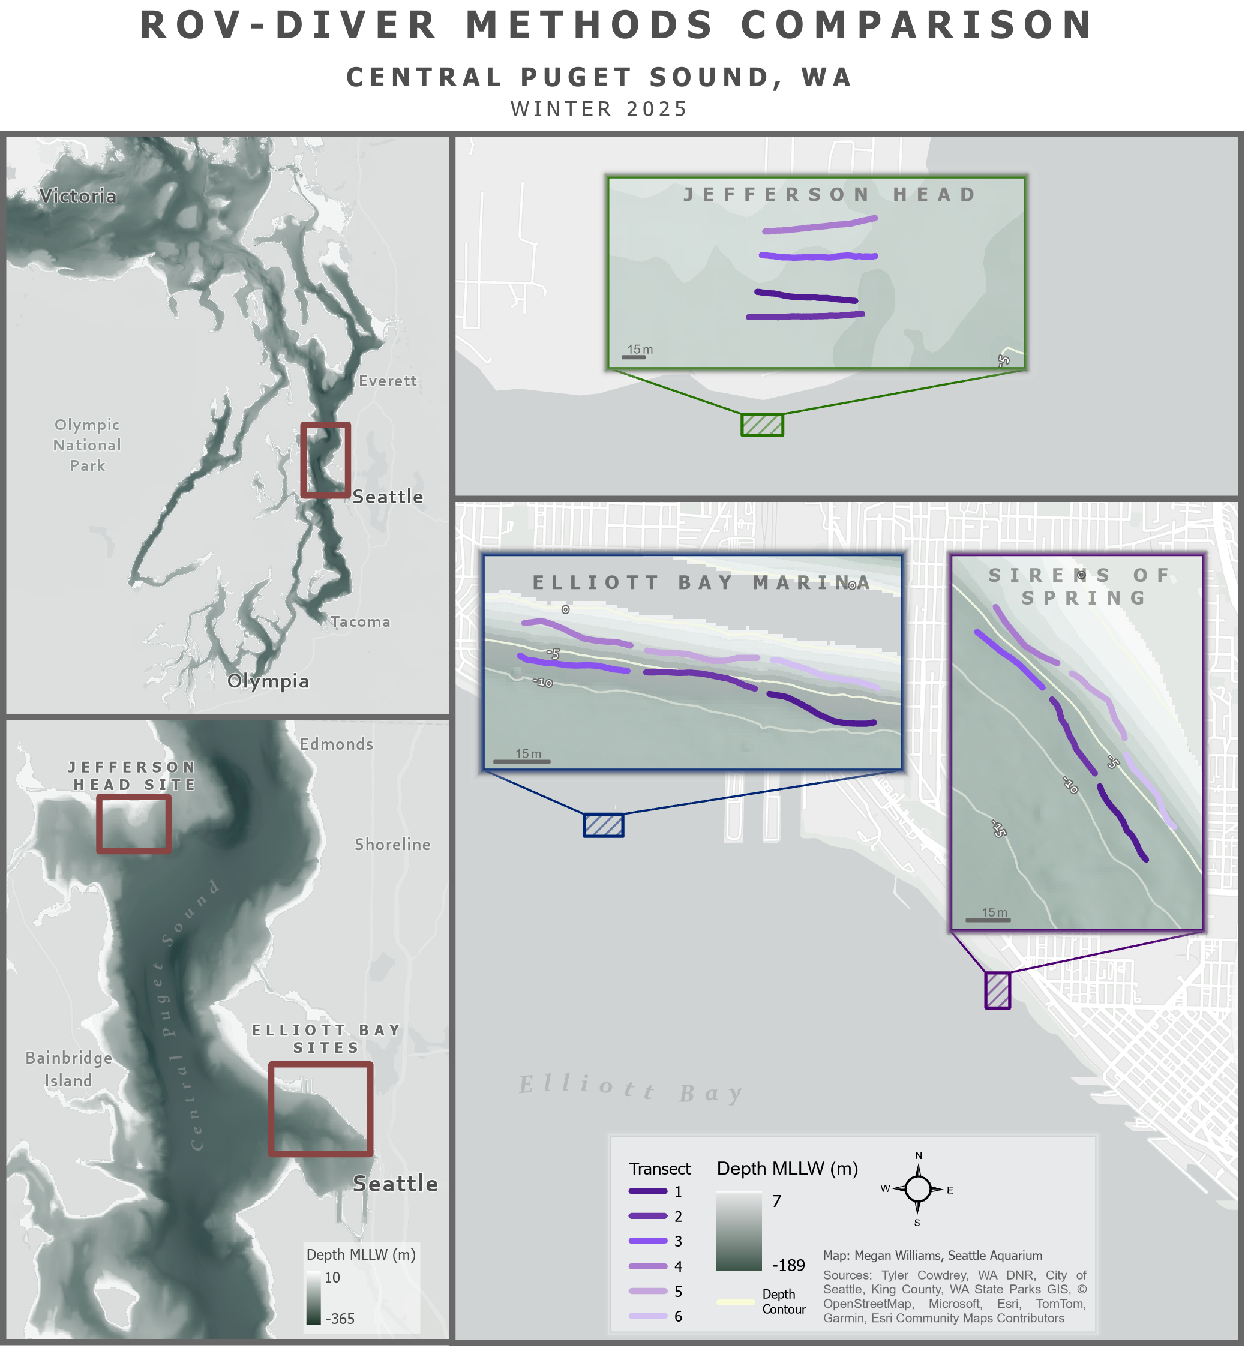
\includegraphics[width=0.85\textwidth]{site_map.pdf}
\caption{
A map of our ROV-diver method comparison sites, including Jefferson Head, 
Indianola, where the ROV monitoring bull kelp restoration with Puget Sound 
Restoration Fund (not part of this technical report).
The two focal sites detailed with this report include Sirens of Spring 
(henceforth referred to as ``Centennial Park''), and the Elliott Bay Marina
breakwater. 
Purple lines denote actual ROV-diver transects as recorded in the ROV's 
telemetry file. 
}
\label{fig:site_map}
\end{figure}
\vfil
}

\clearpage

\vbox to \textheight{%
\vfil
\begin{figure}[H]
\centering
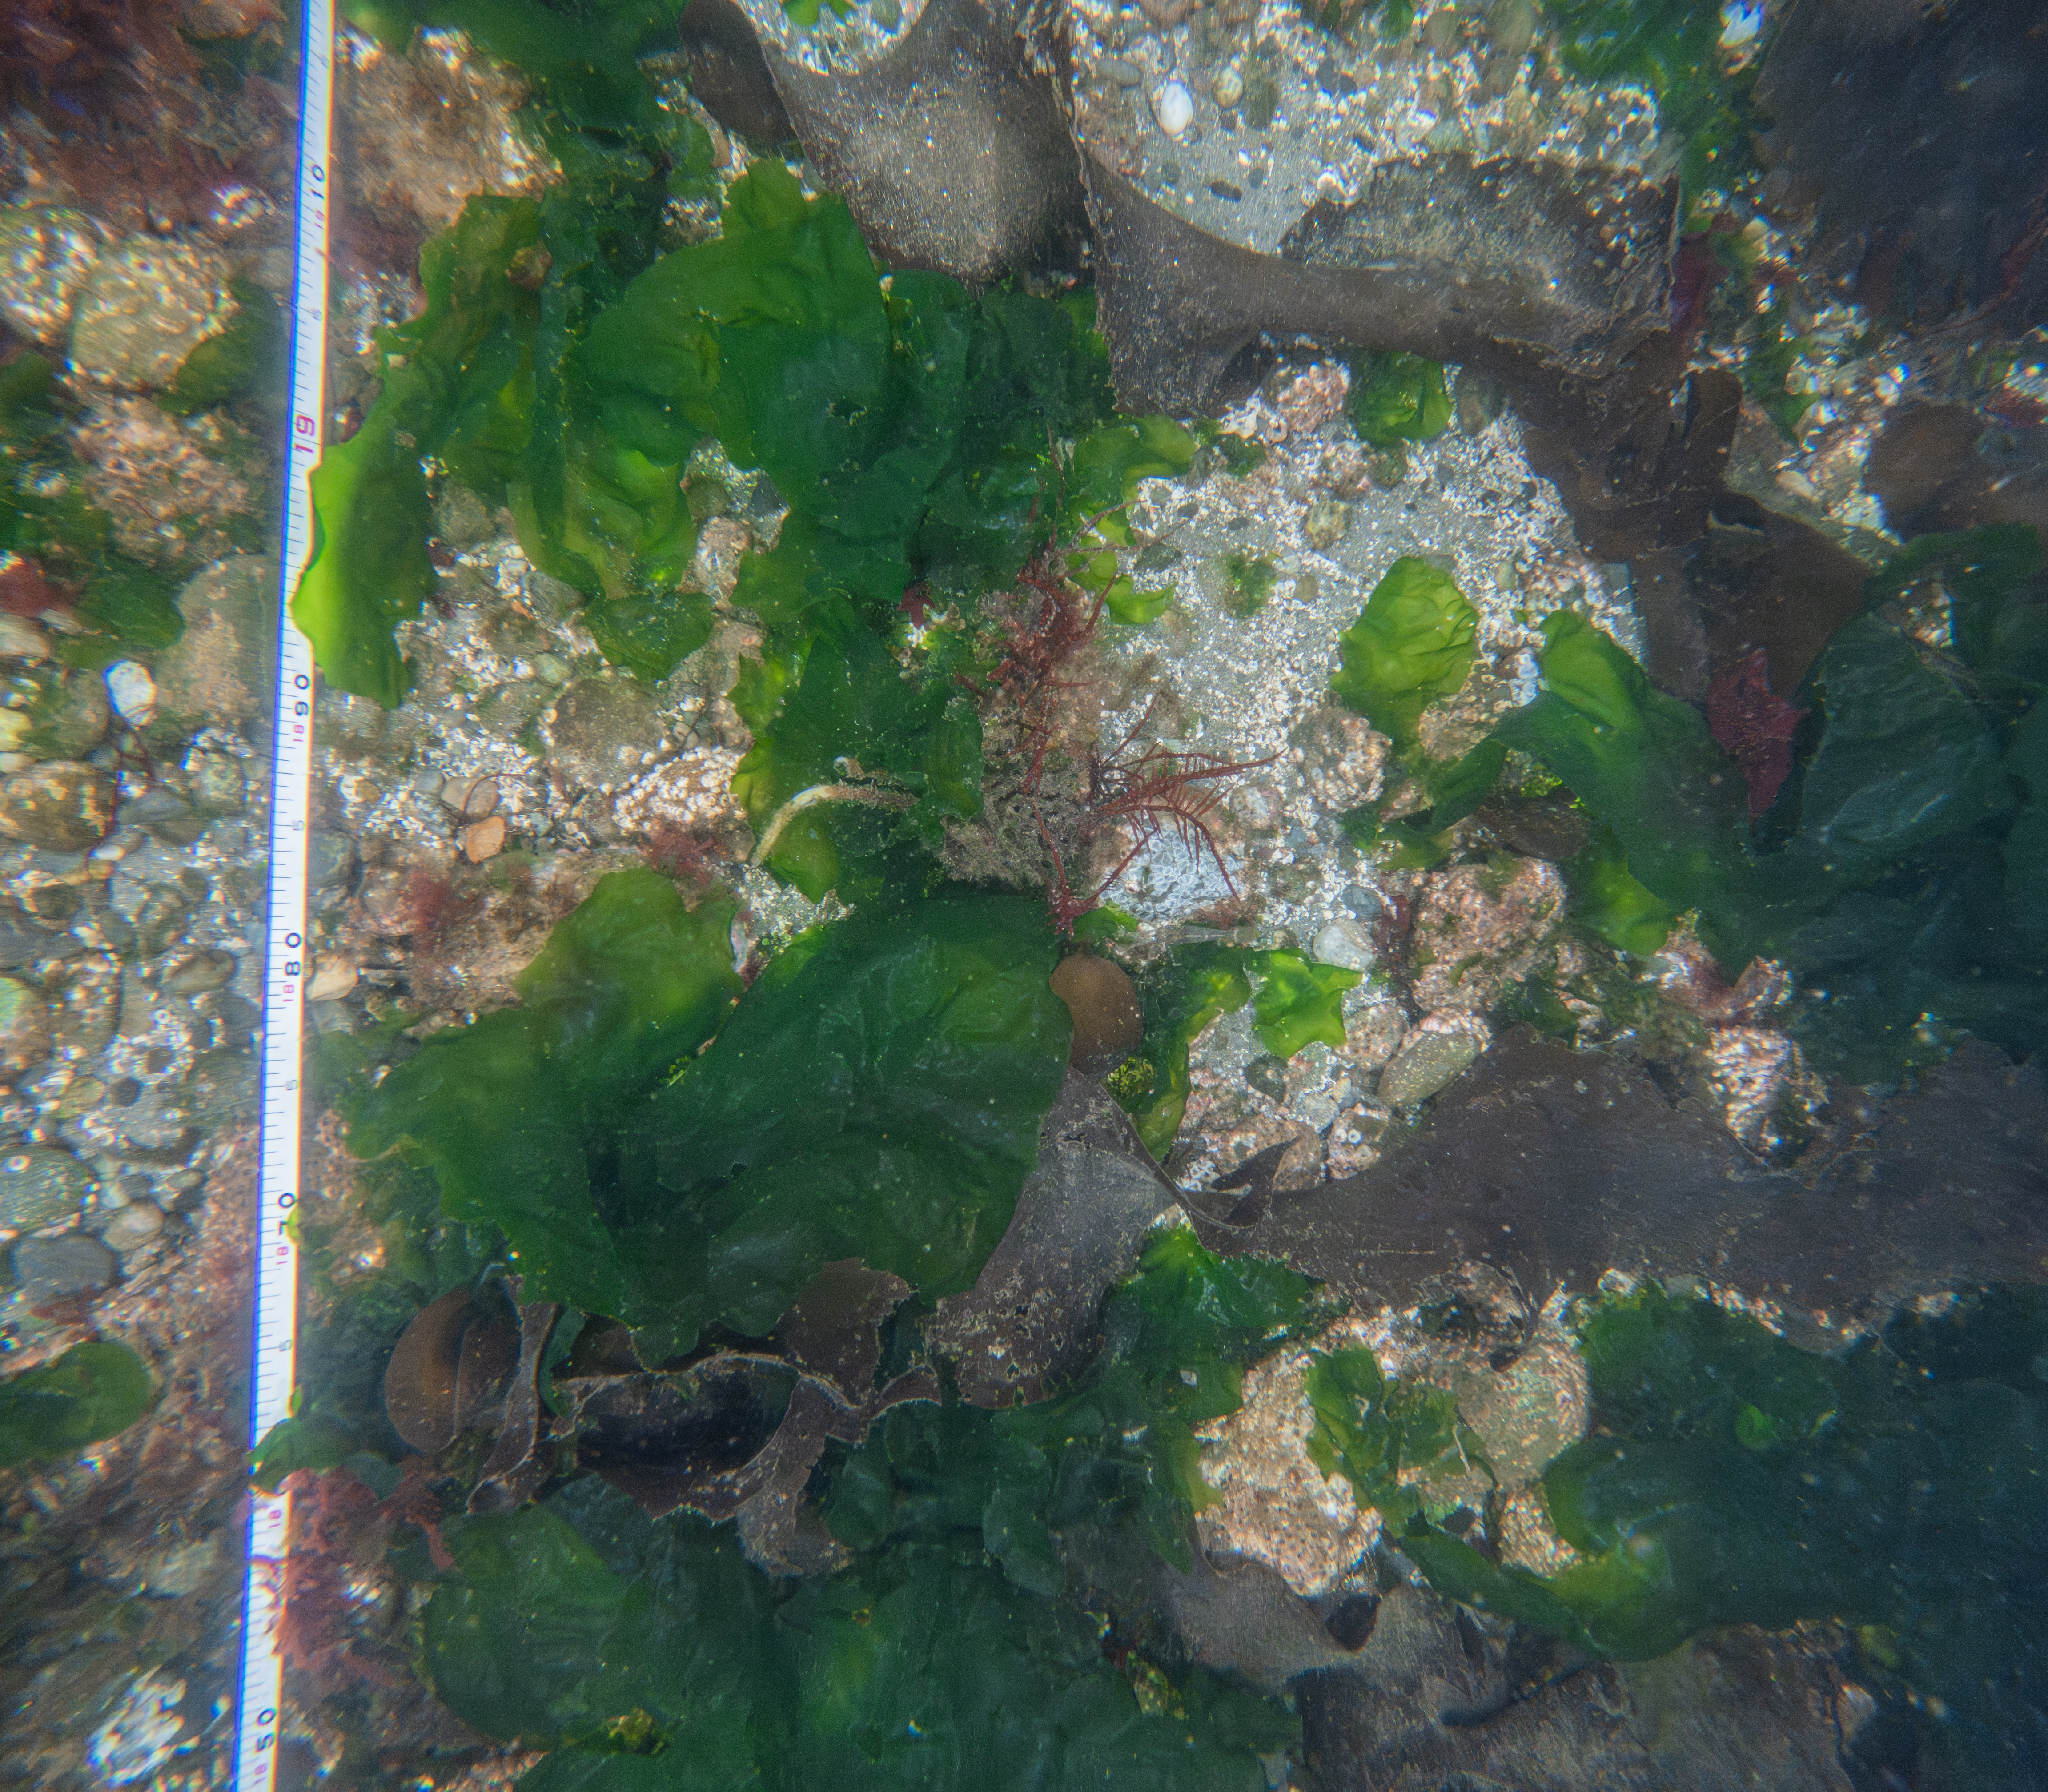
\includegraphics[width=0.326\textwidth]{CP_shallow_1.jpg}%
\hspace{0.005\textwidth}%
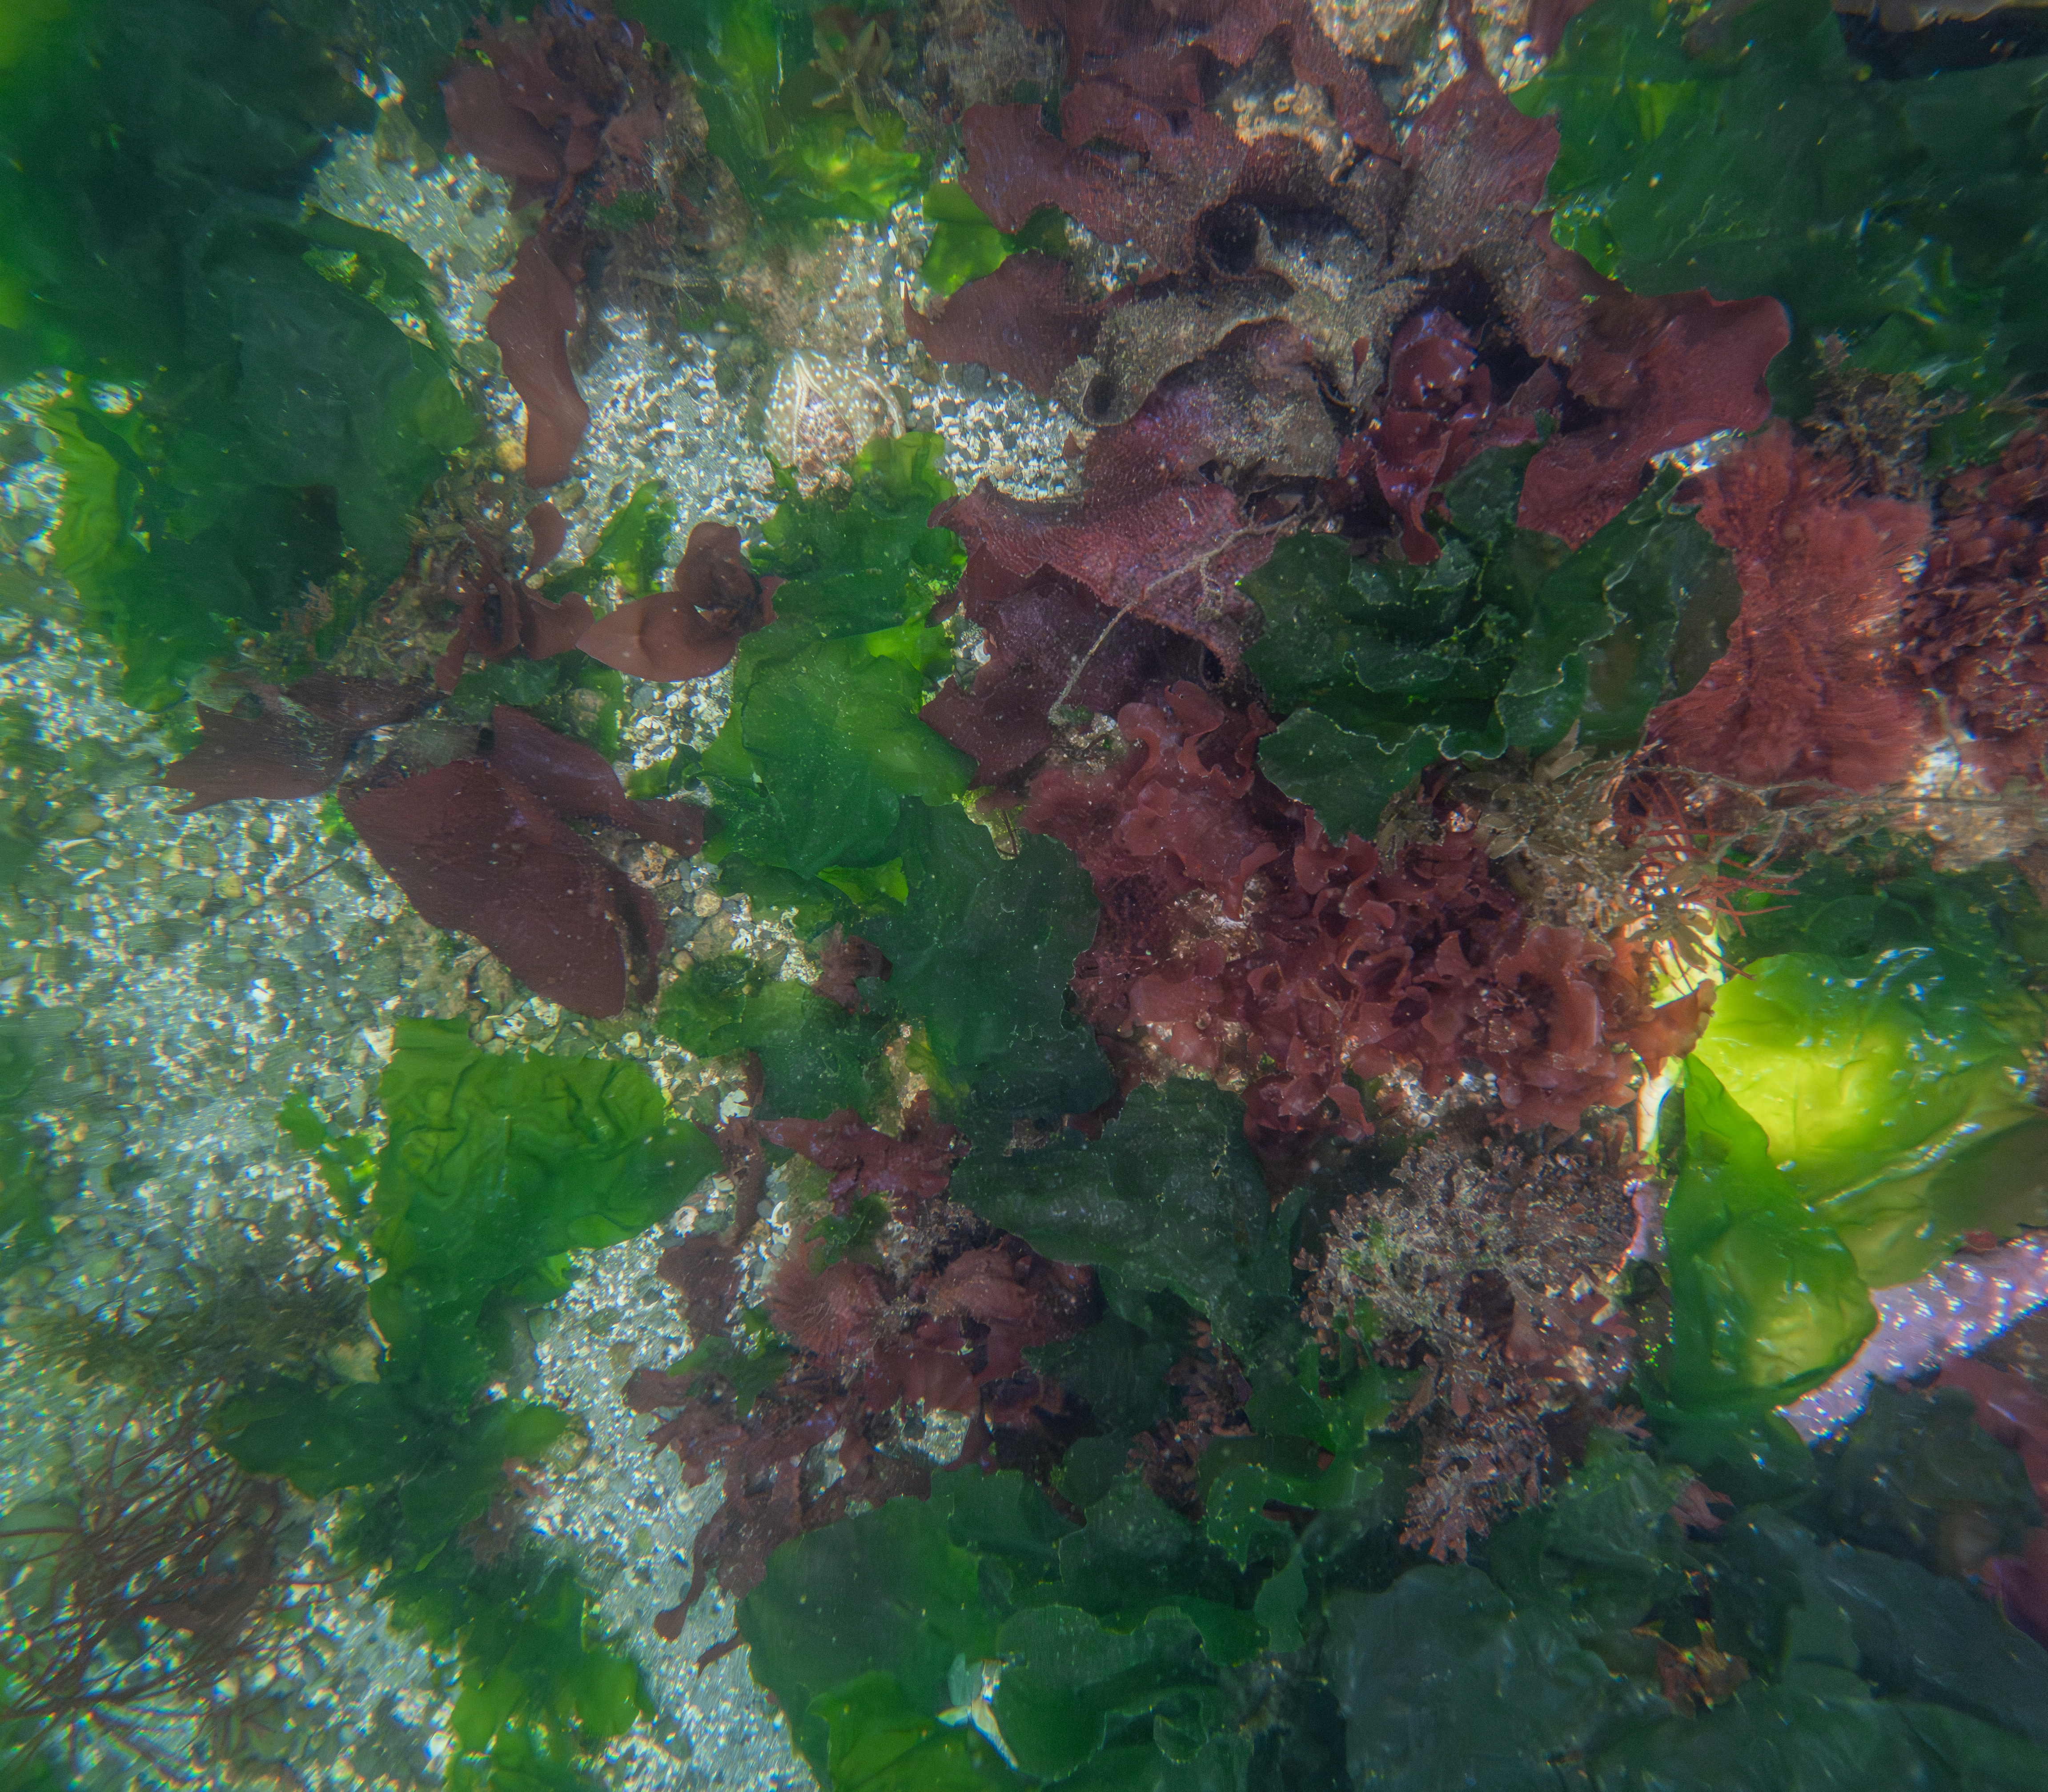
\includegraphics[width=0.326\textwidth]{CP_shallow_2.jpg}%
\hspace{0.005\textwidth}%
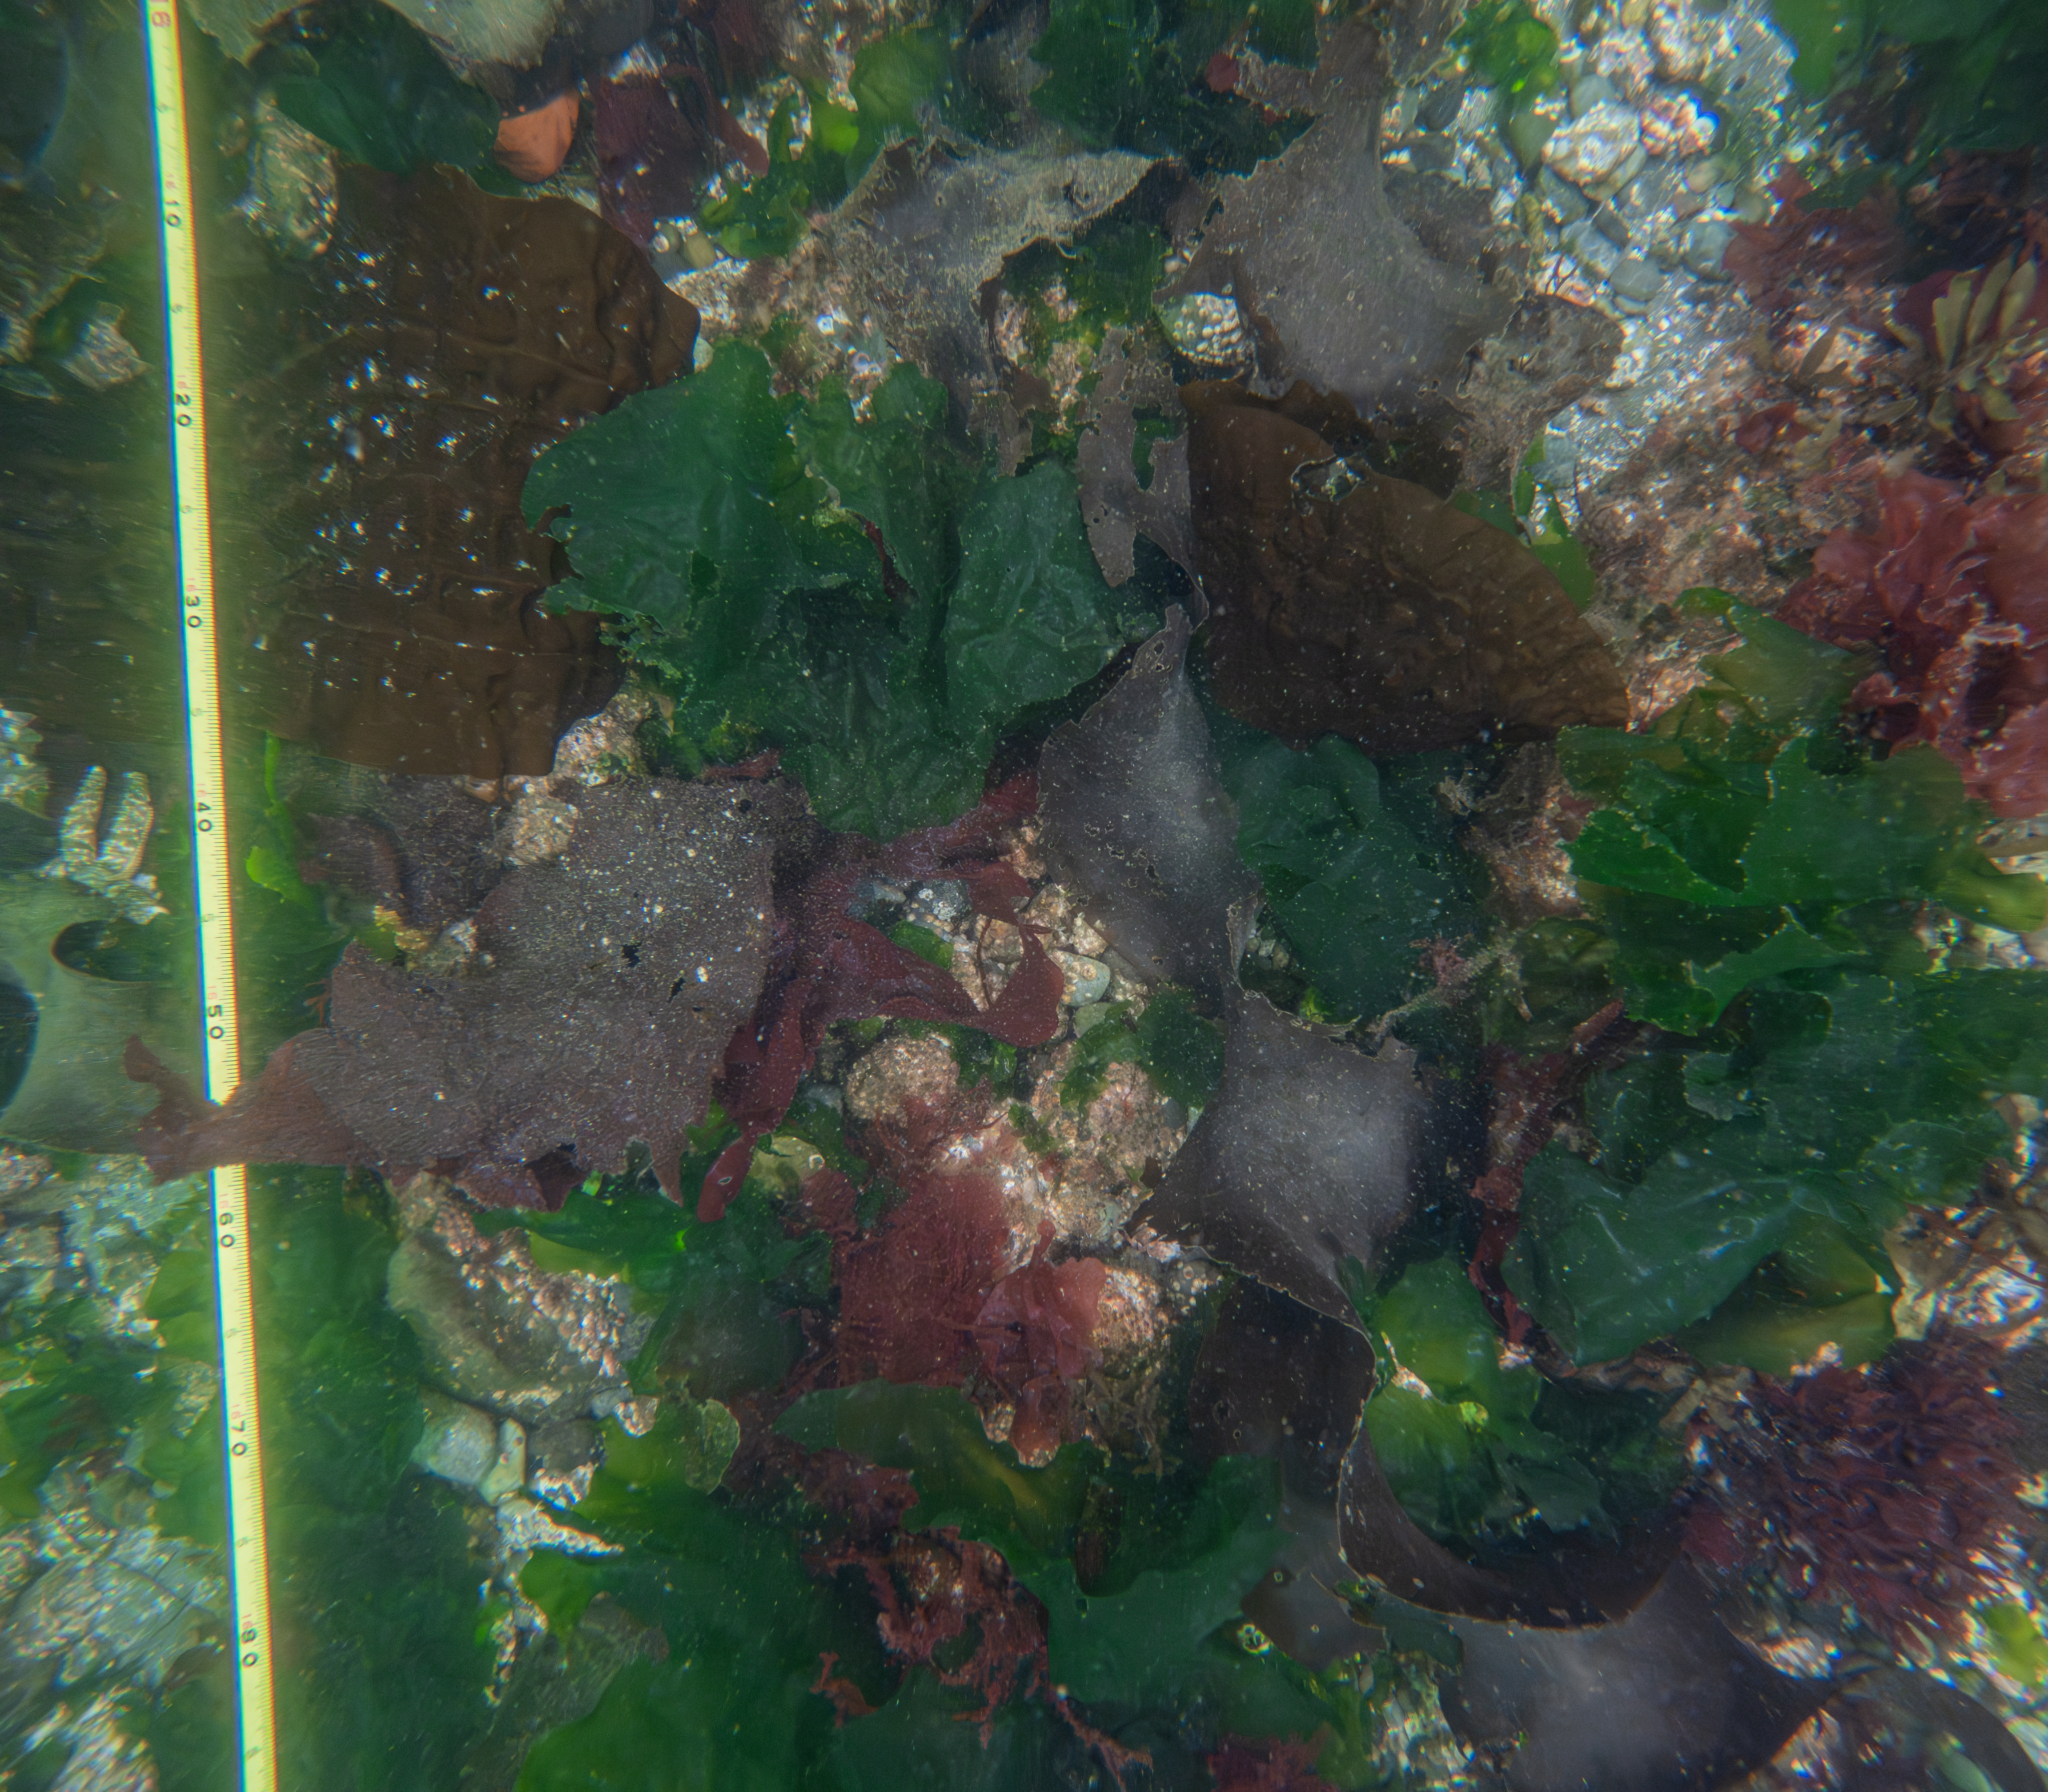
\includegraphics[width=0.326\textwidth]{CP_shallow_3.jpg}\par
\vspace{0.005\textwidth}
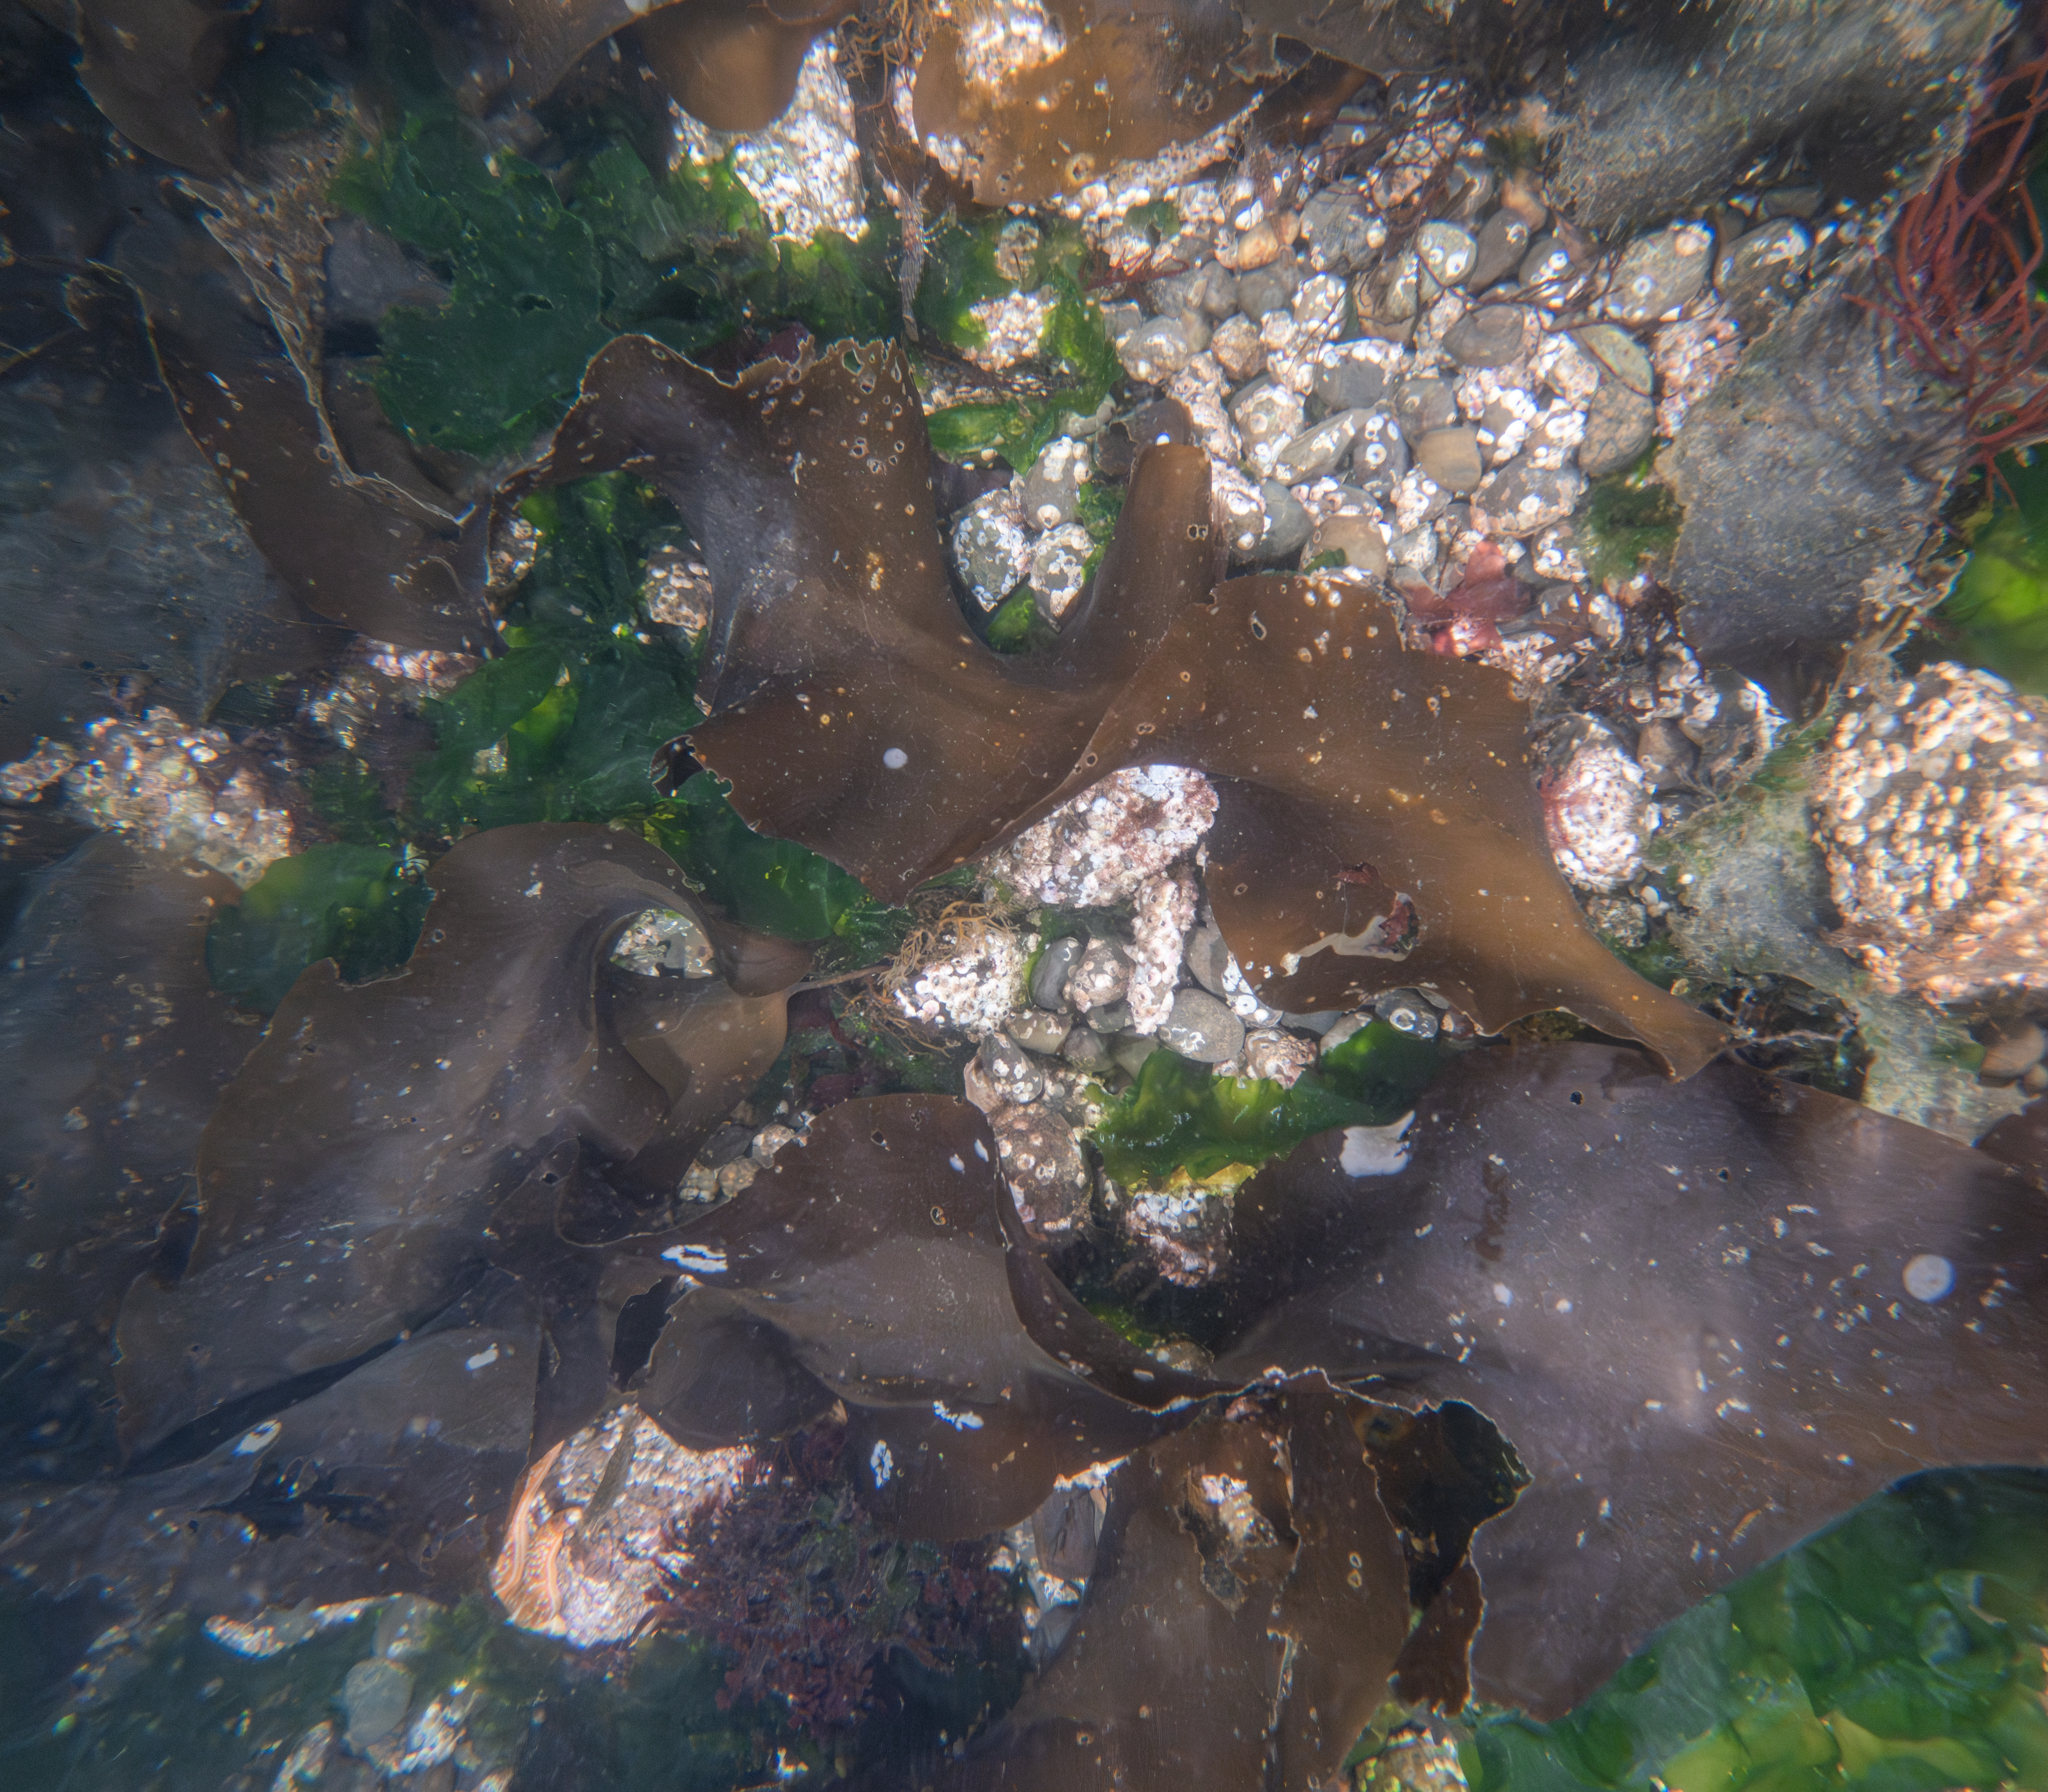
\includegraphics[width=0.326\textwidth]{CP_deep_1.jpg}%
\hspace{0.005\textwidth}%
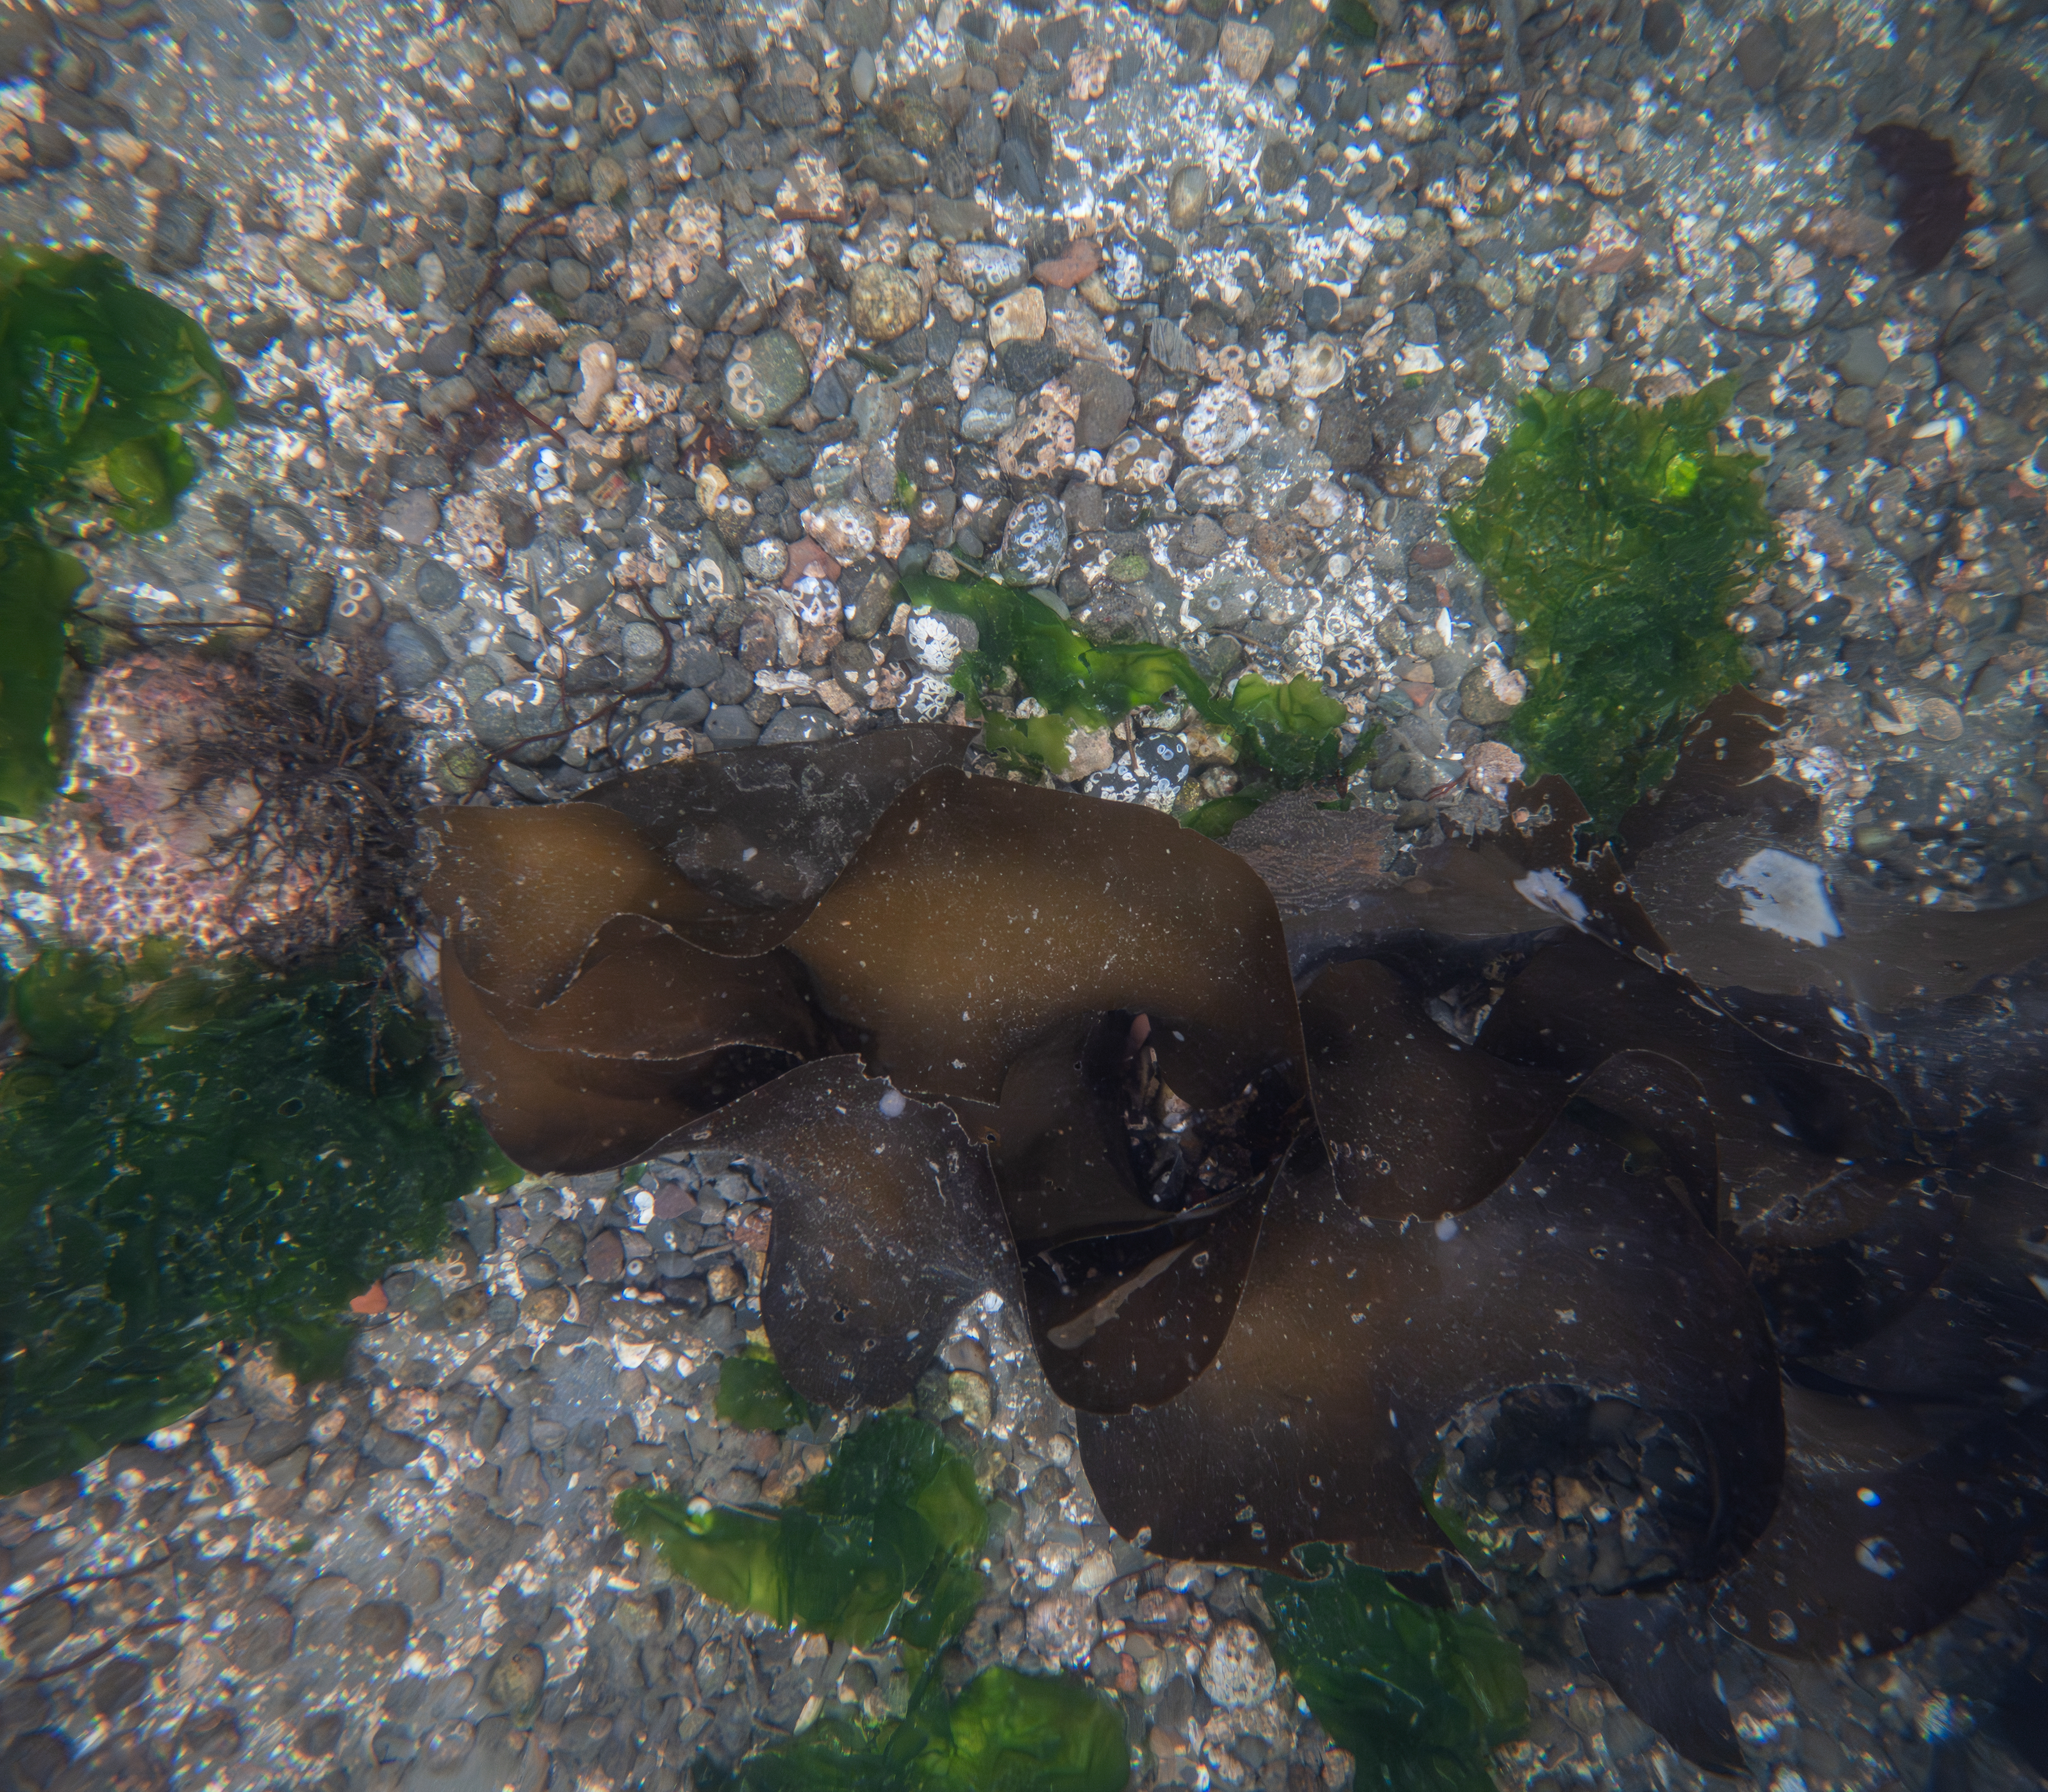
\includegraphics[width=0.326\textwidth]{CP_deep_2.jpg}%
\hspace{0.005\textwidth}%
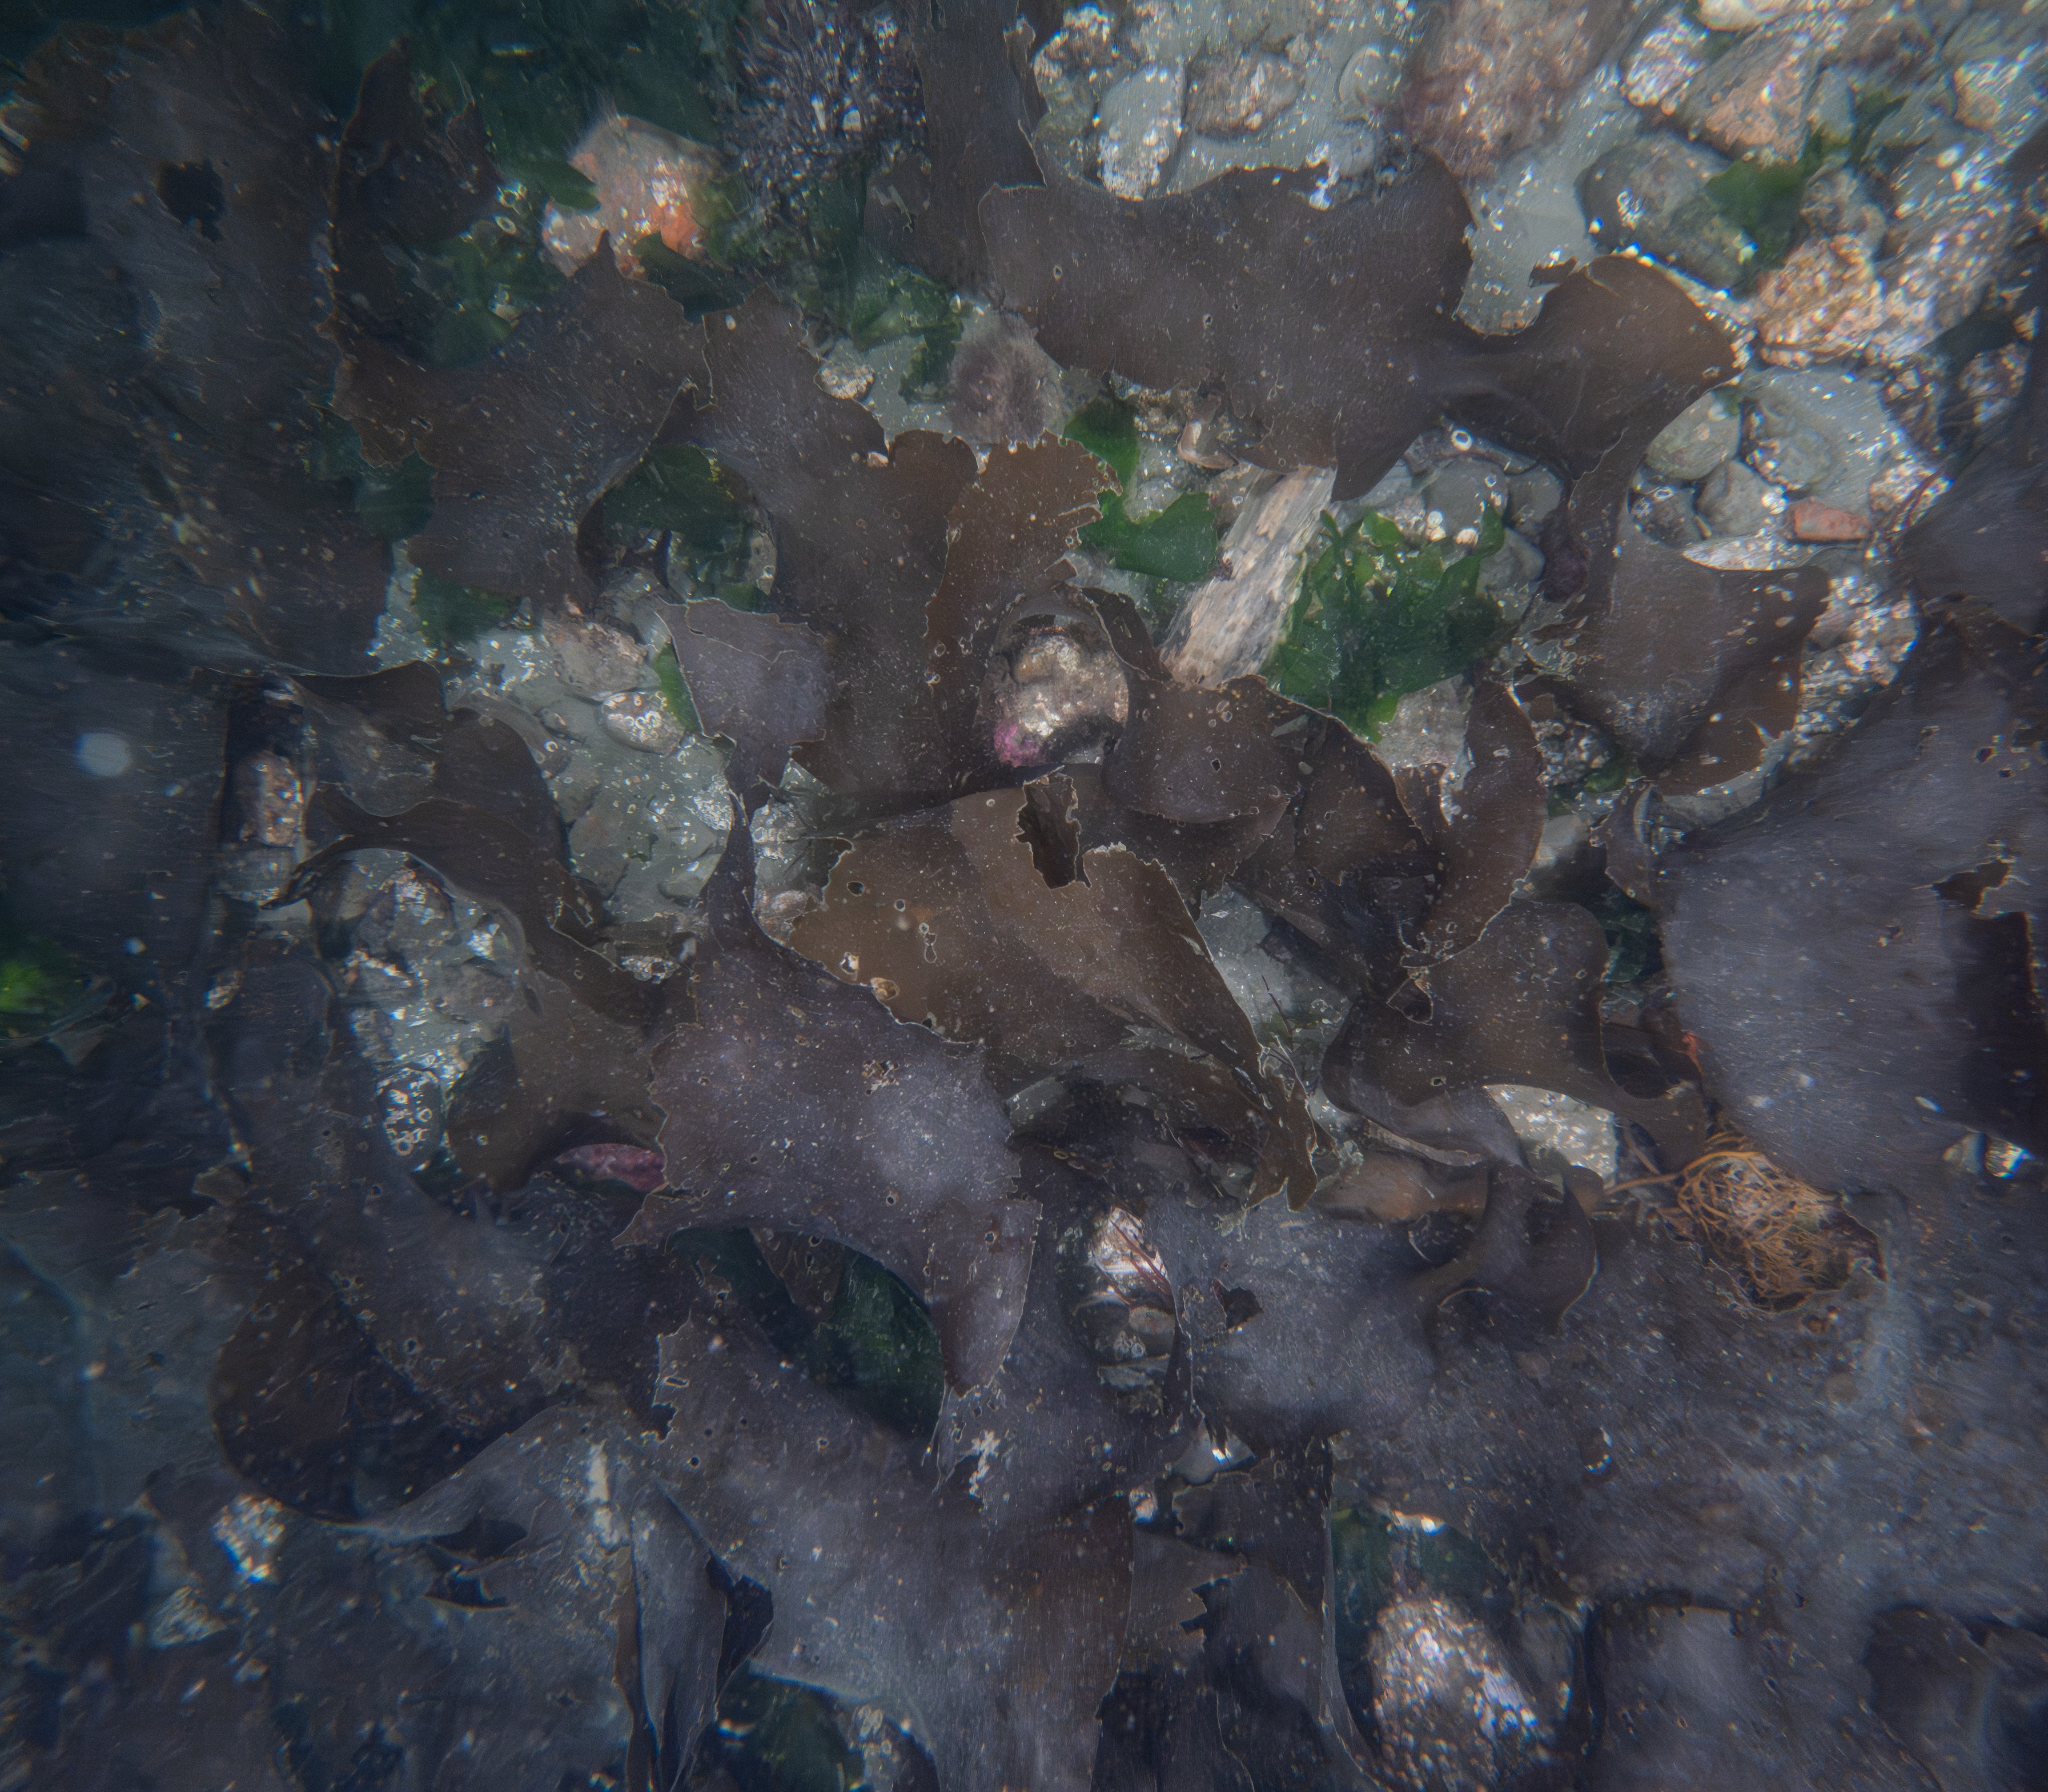
\includegraphics[width=0.326\textwidth]{CP_deep_3.jpg}\par
\vspace{0.005\textwidth}
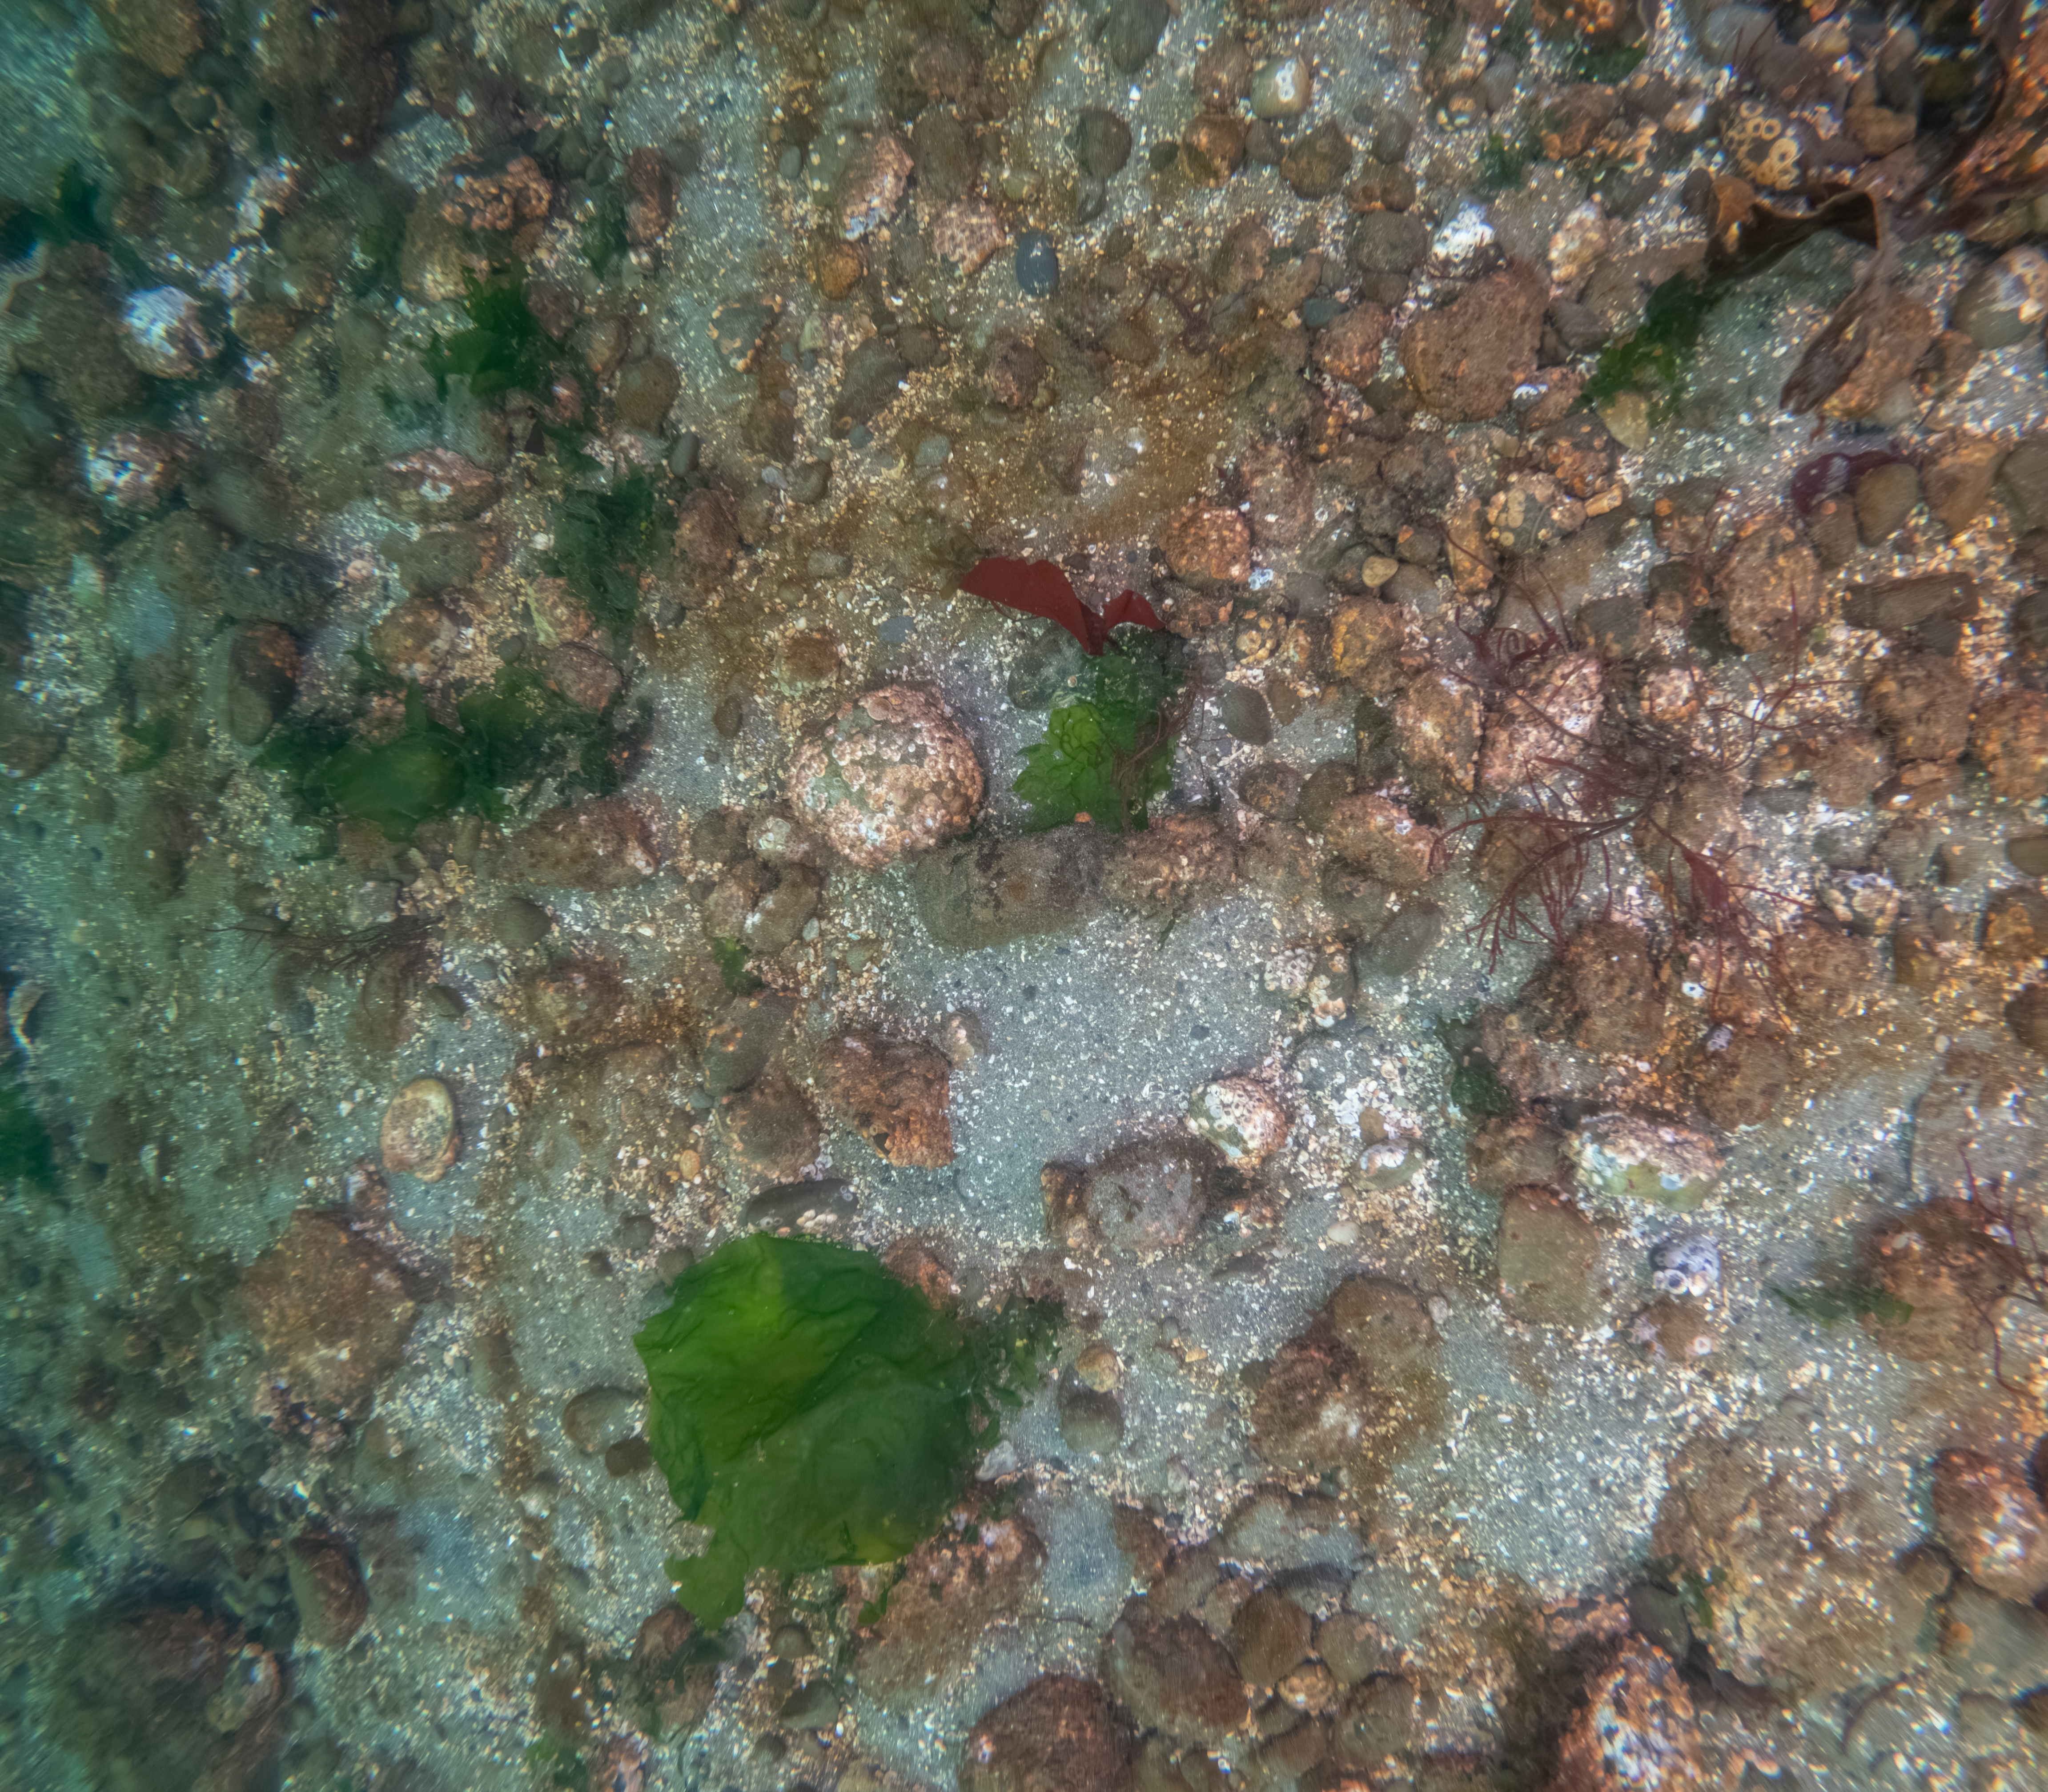
\includegraphics[width=0.326\textwidth]{CP_winter_1.jpg}%
\hspace{0.005\textwidth}%
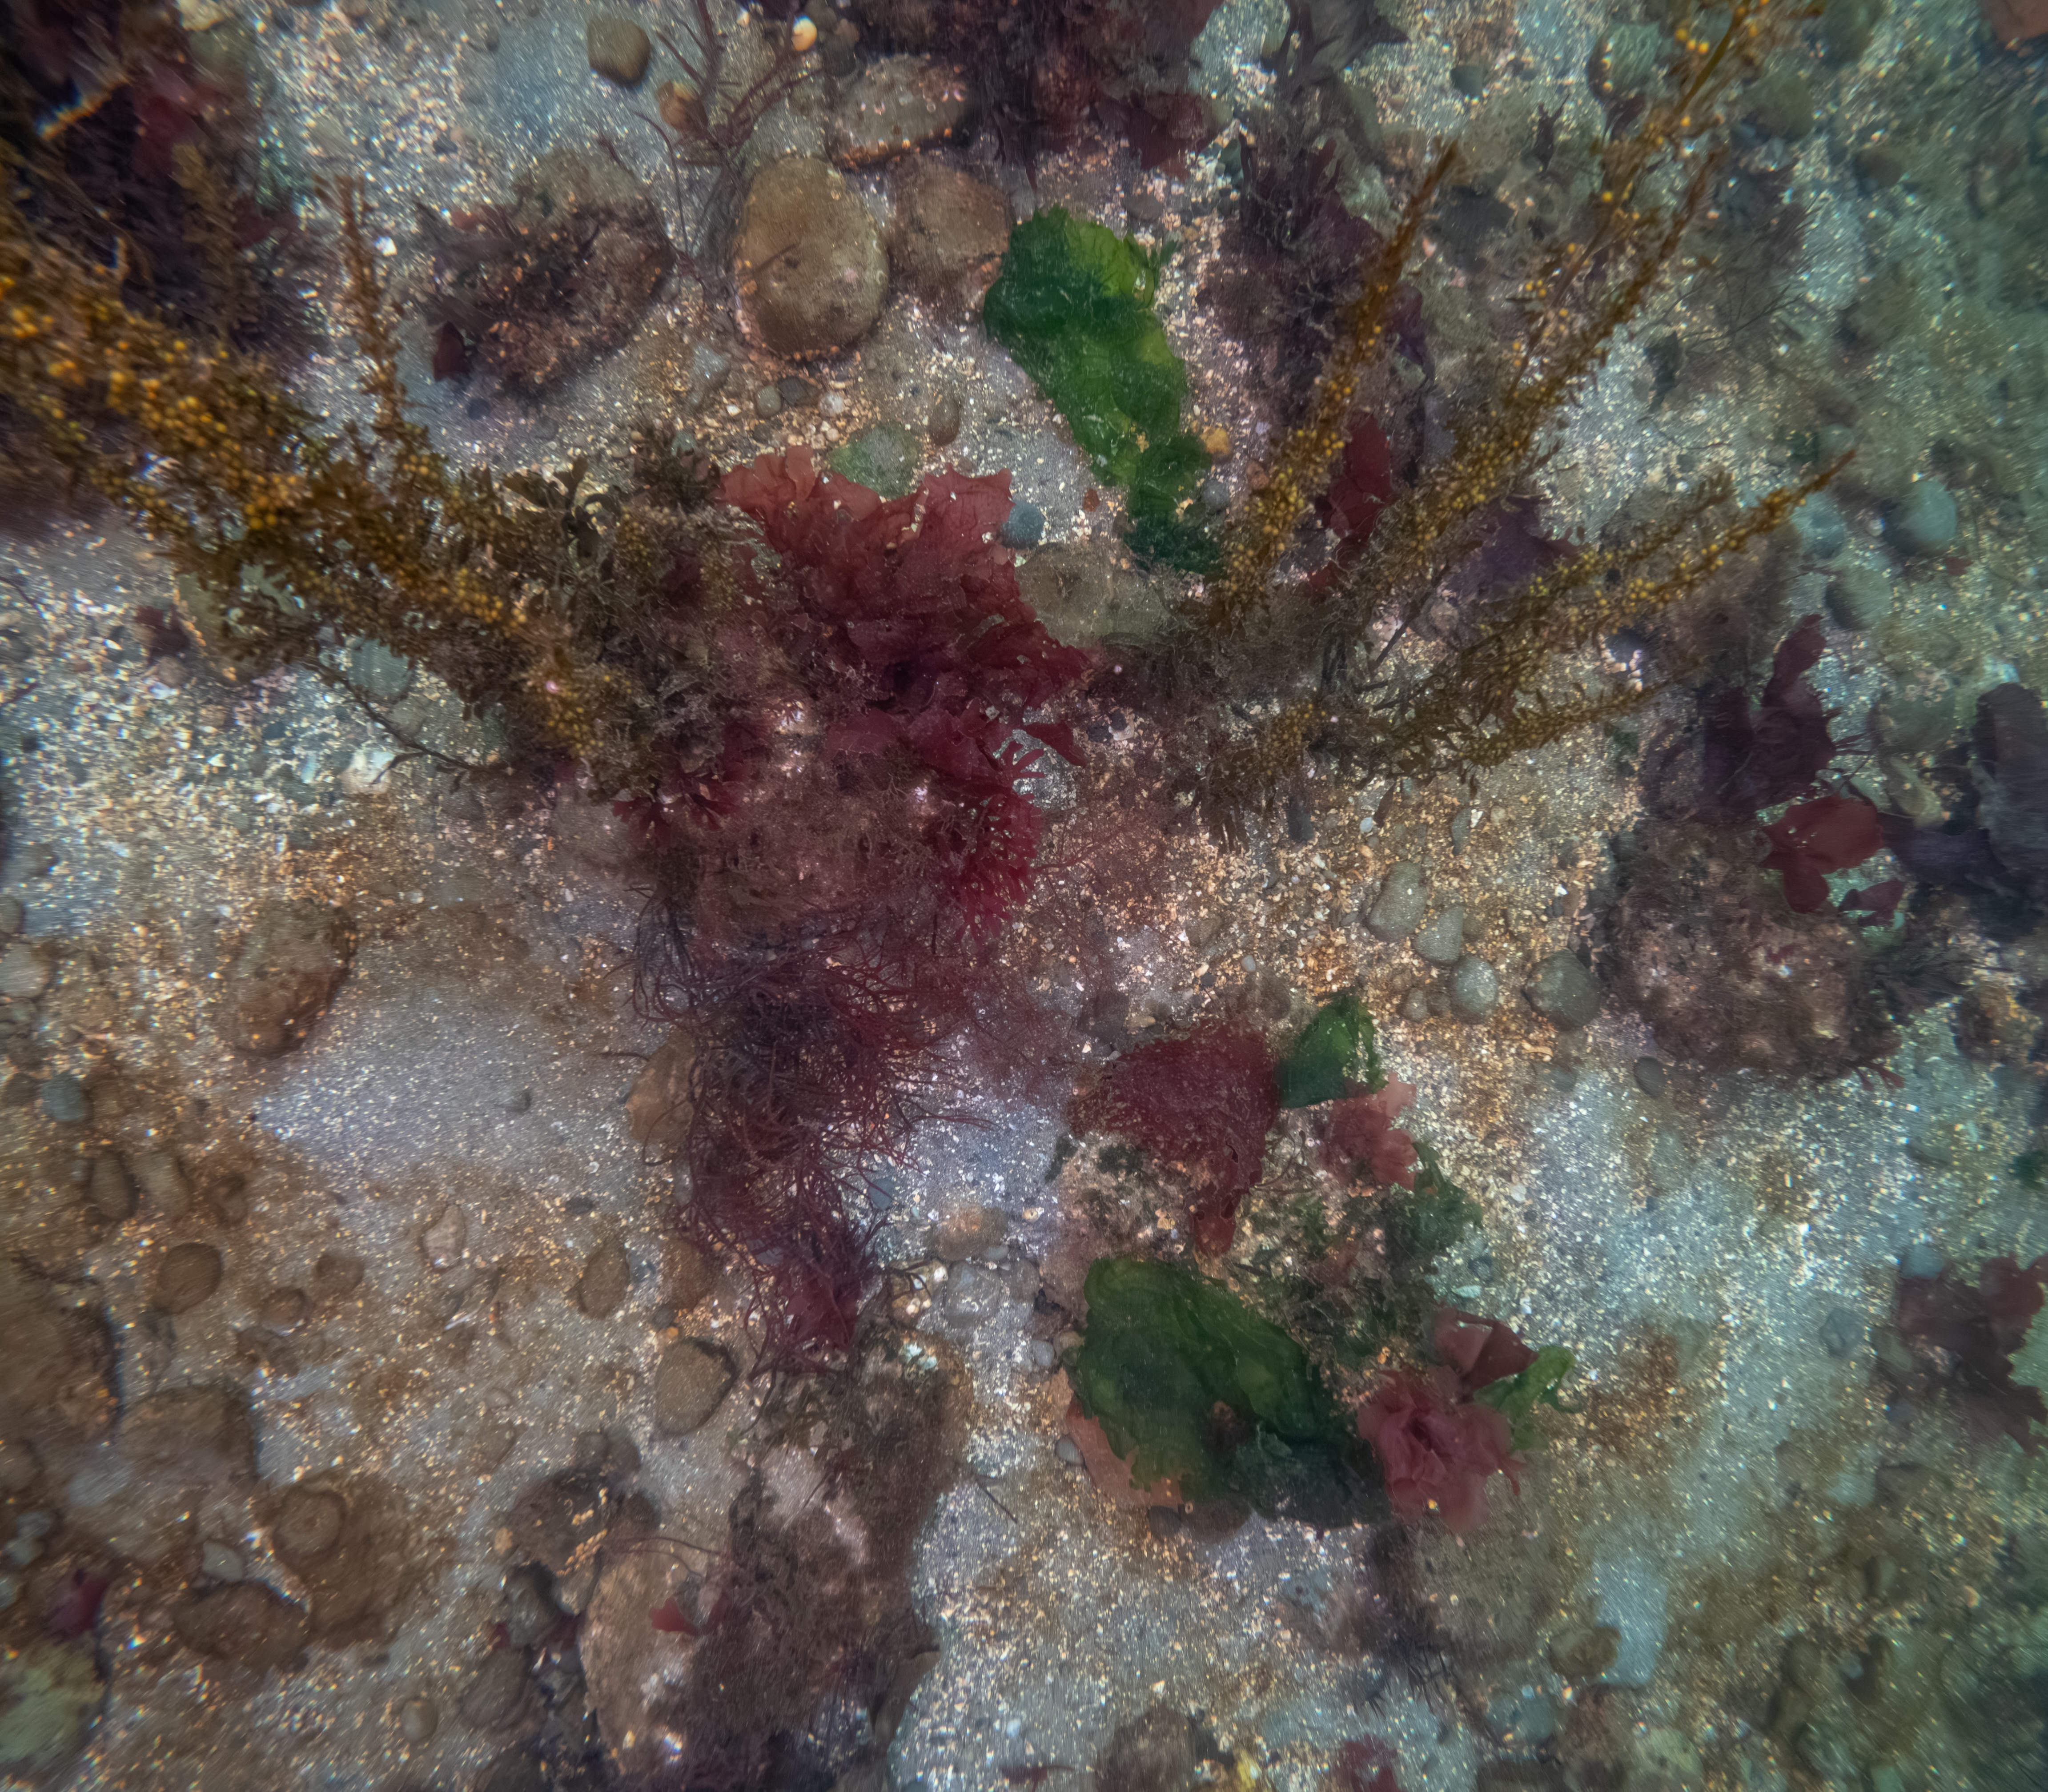
\includegraphics[width=0.326\textwidth]{CP_winter_2.jpg}%
\hspace{0.005\textwidth}%
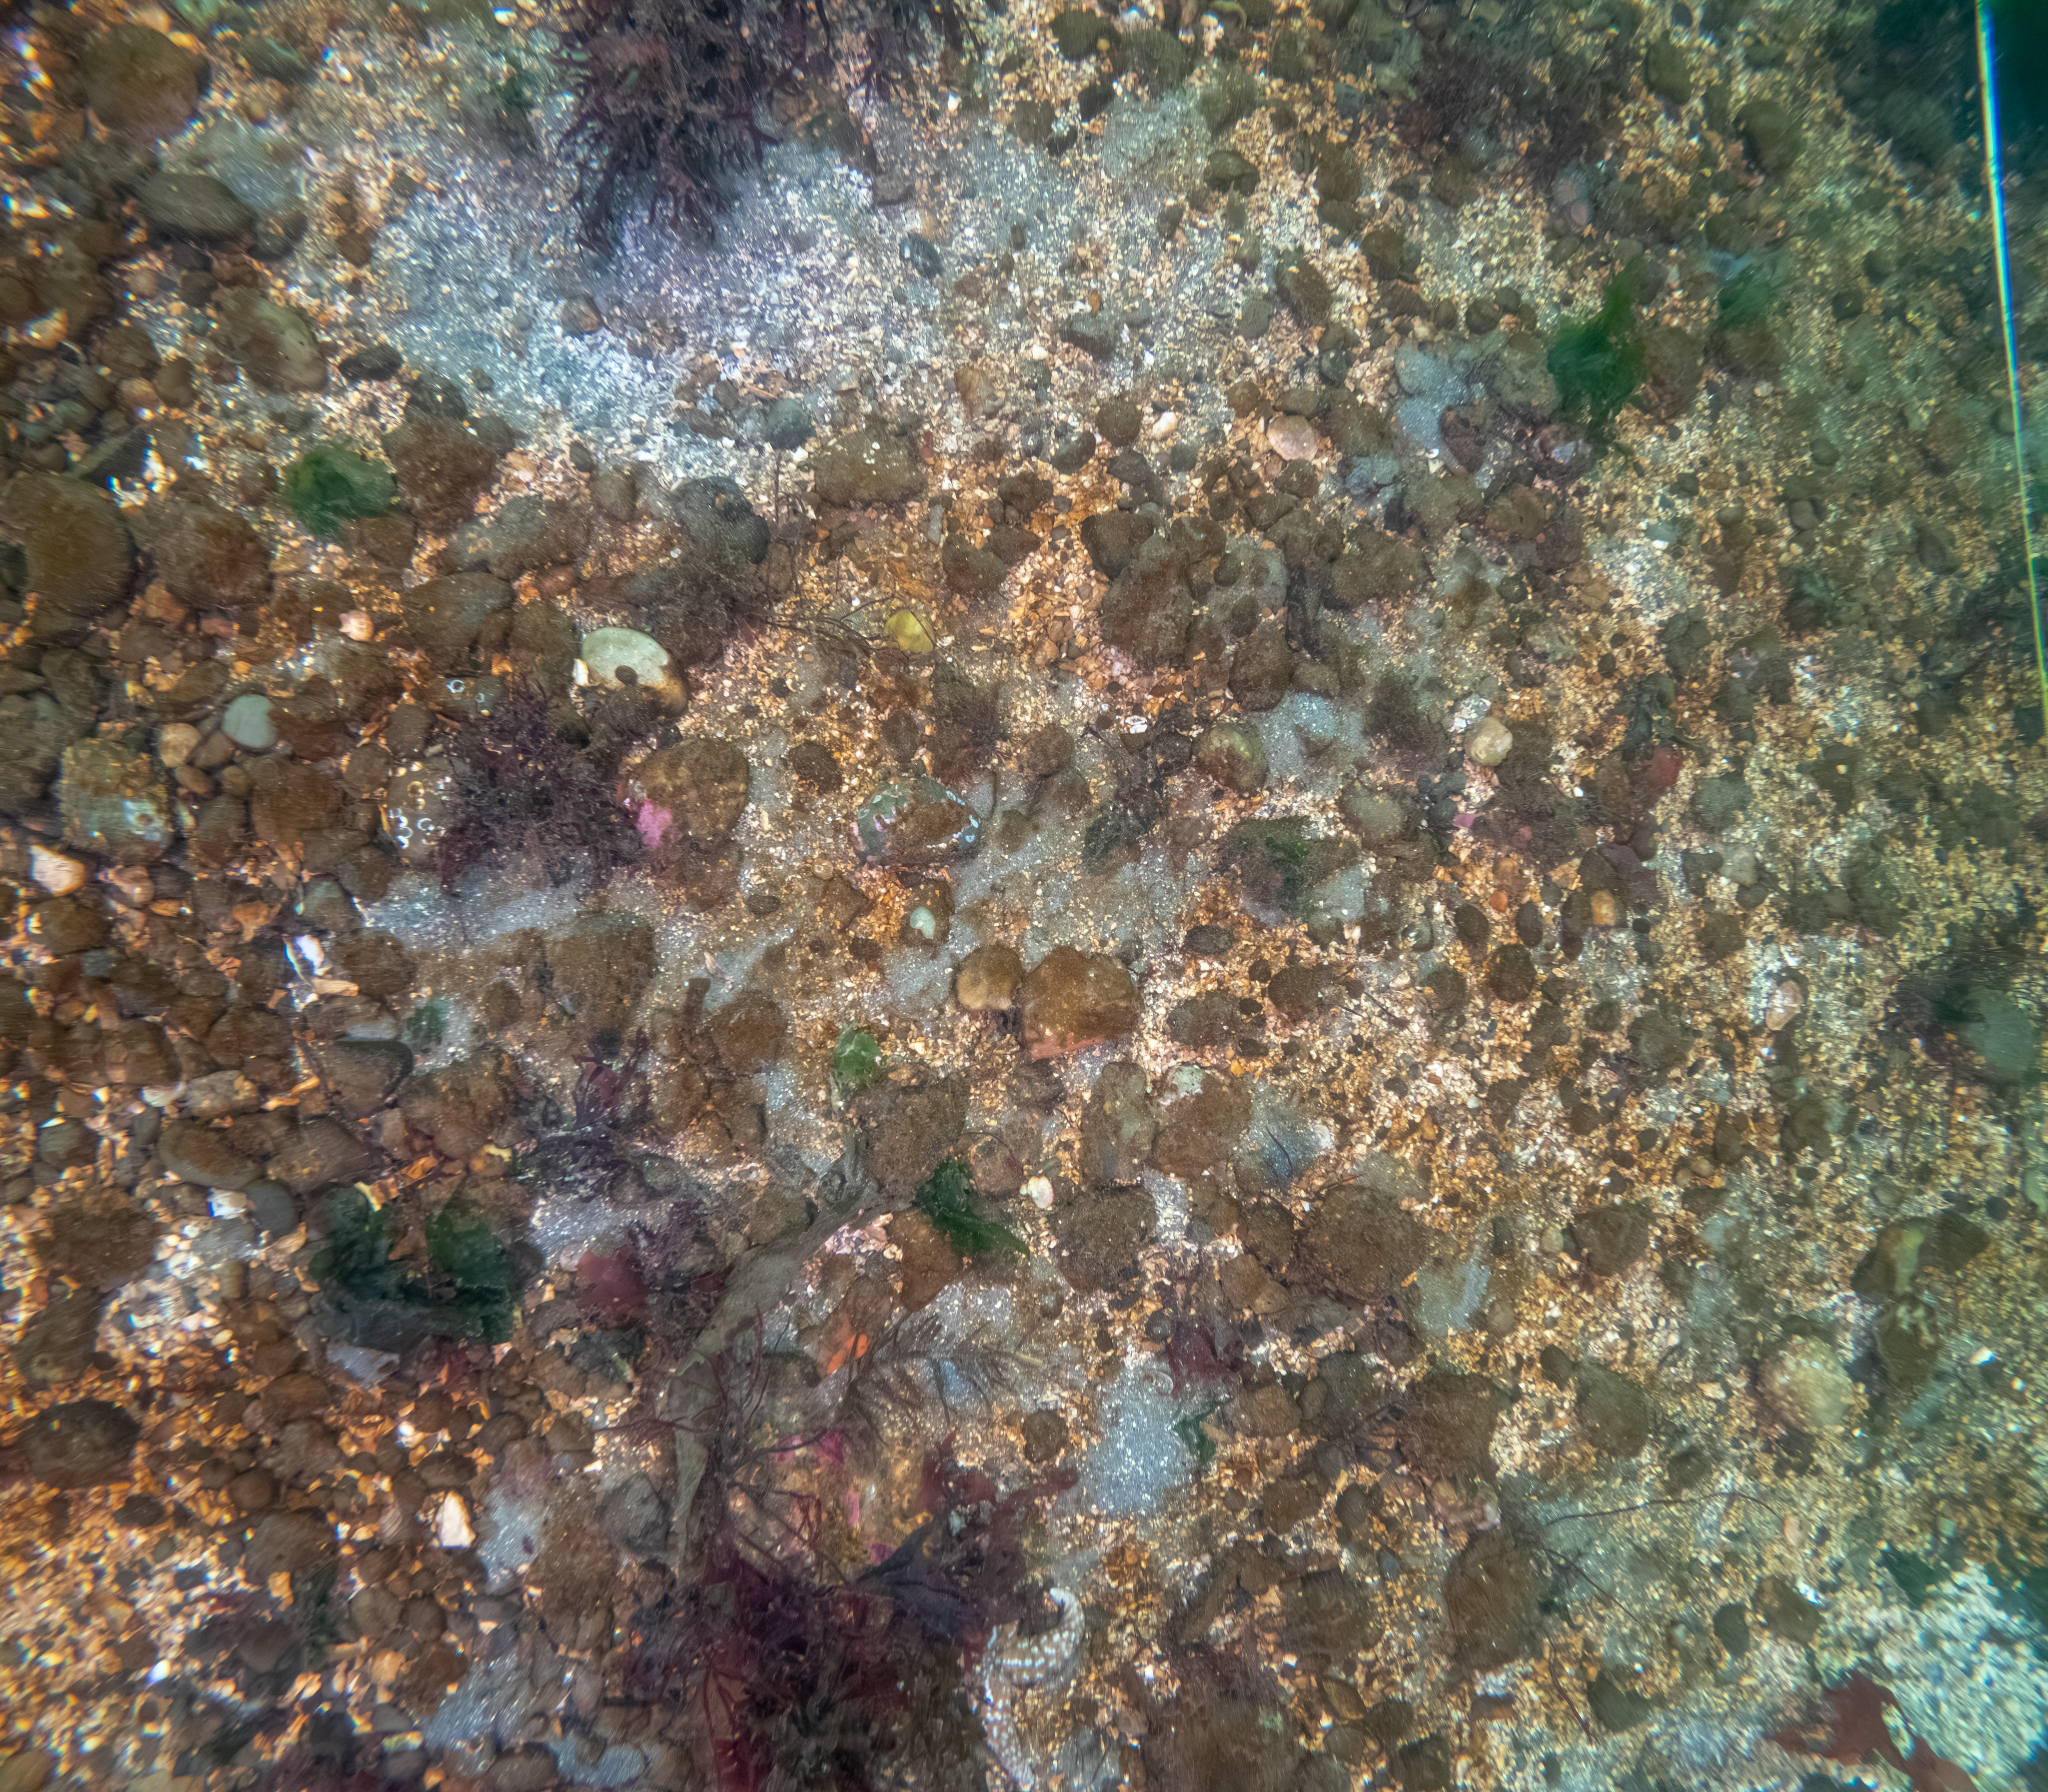
\includegraphics[width=0.326\textwidth]{CP_winter_3.jpg}
\caption{
Nine example ROV survey images from Centennial Park. 
Row 1 depicts three images from the shallow transects ($5~m$ depth) in the 
summer of 2024;
Row 2 depicts three images from the deep transects ($10~m$ depth) in the summer 
of 2024;
Row 3 depicts three images from the winter of 2025 (both depths).
Centennial Park consists of soft-sediment with pebble/cobble rocks, and a 
variety of brown, red, and green algae;
Sugar kelp (\textit{Saccharina latissima}) is the predominant kelp found at 
this site. 
}
\label{fig:CP}
\end{figure}
\vfil
}

\clearpage

\vbox to \textheight{%
\vfil
\begin{figure}[H]
\centering
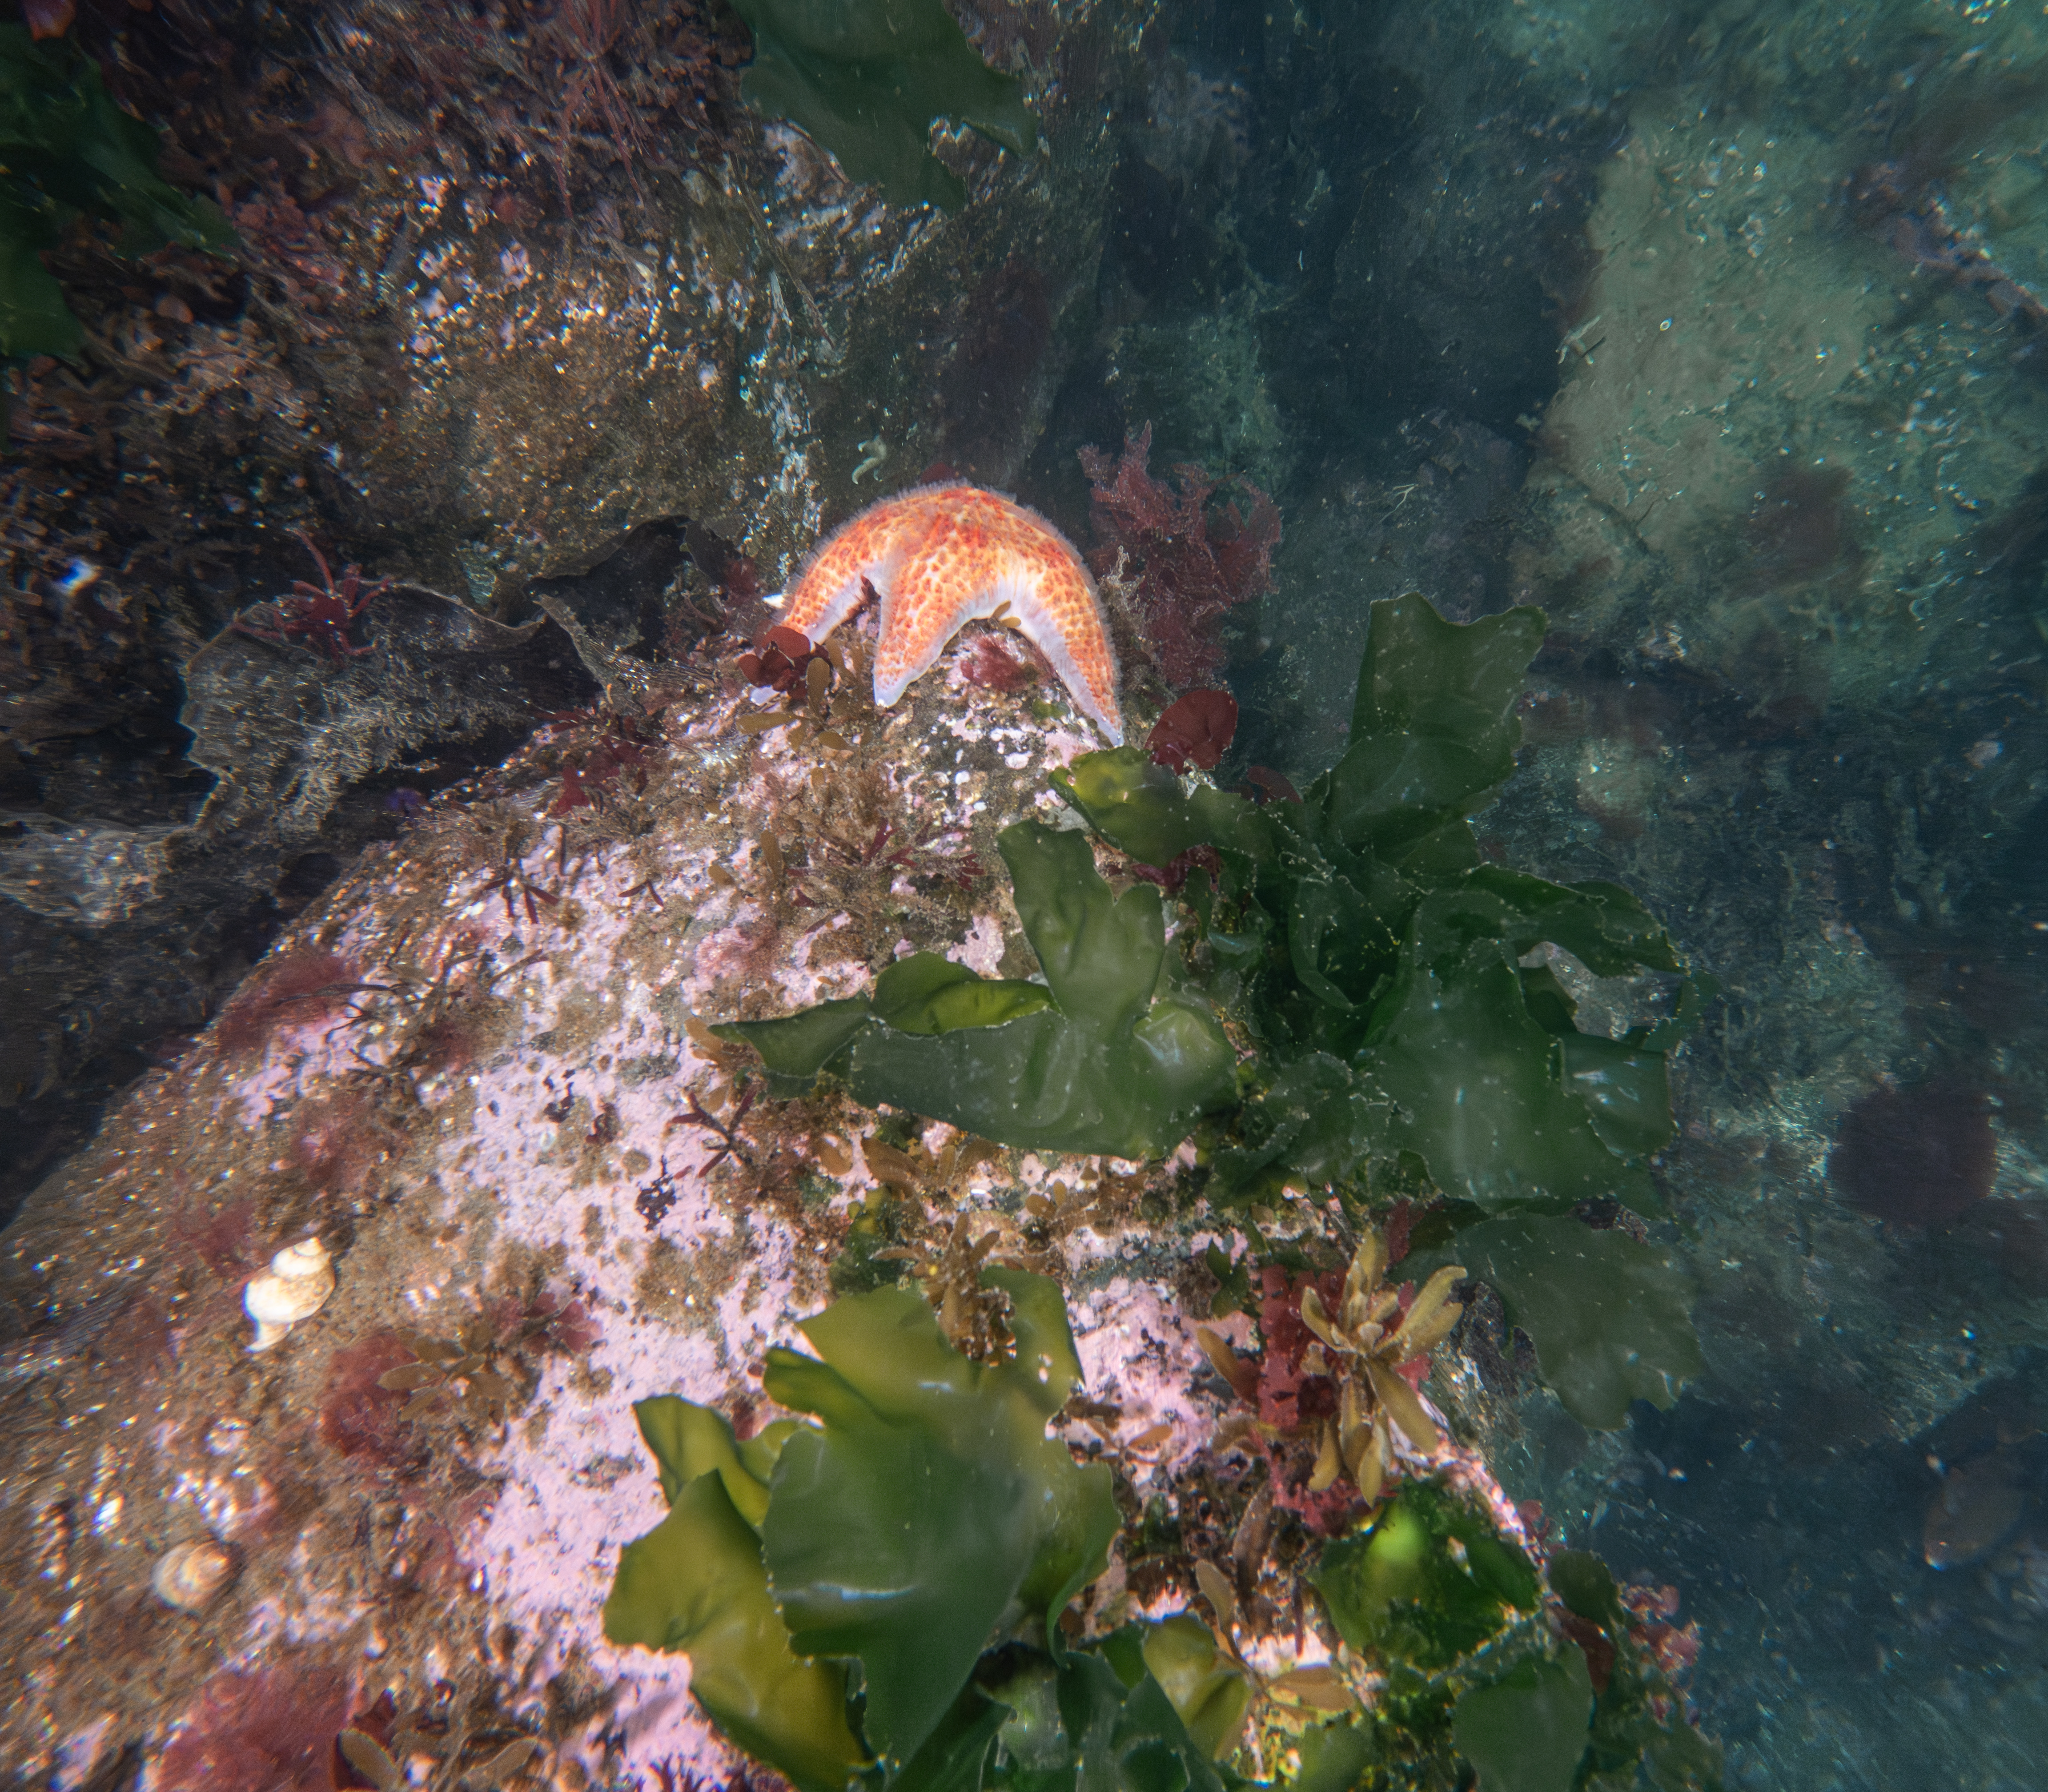
\includegraphics[width=0.326\textwidth]{EBM_shallow_1.jpg}%
\hspace{0.005\textwidth}%
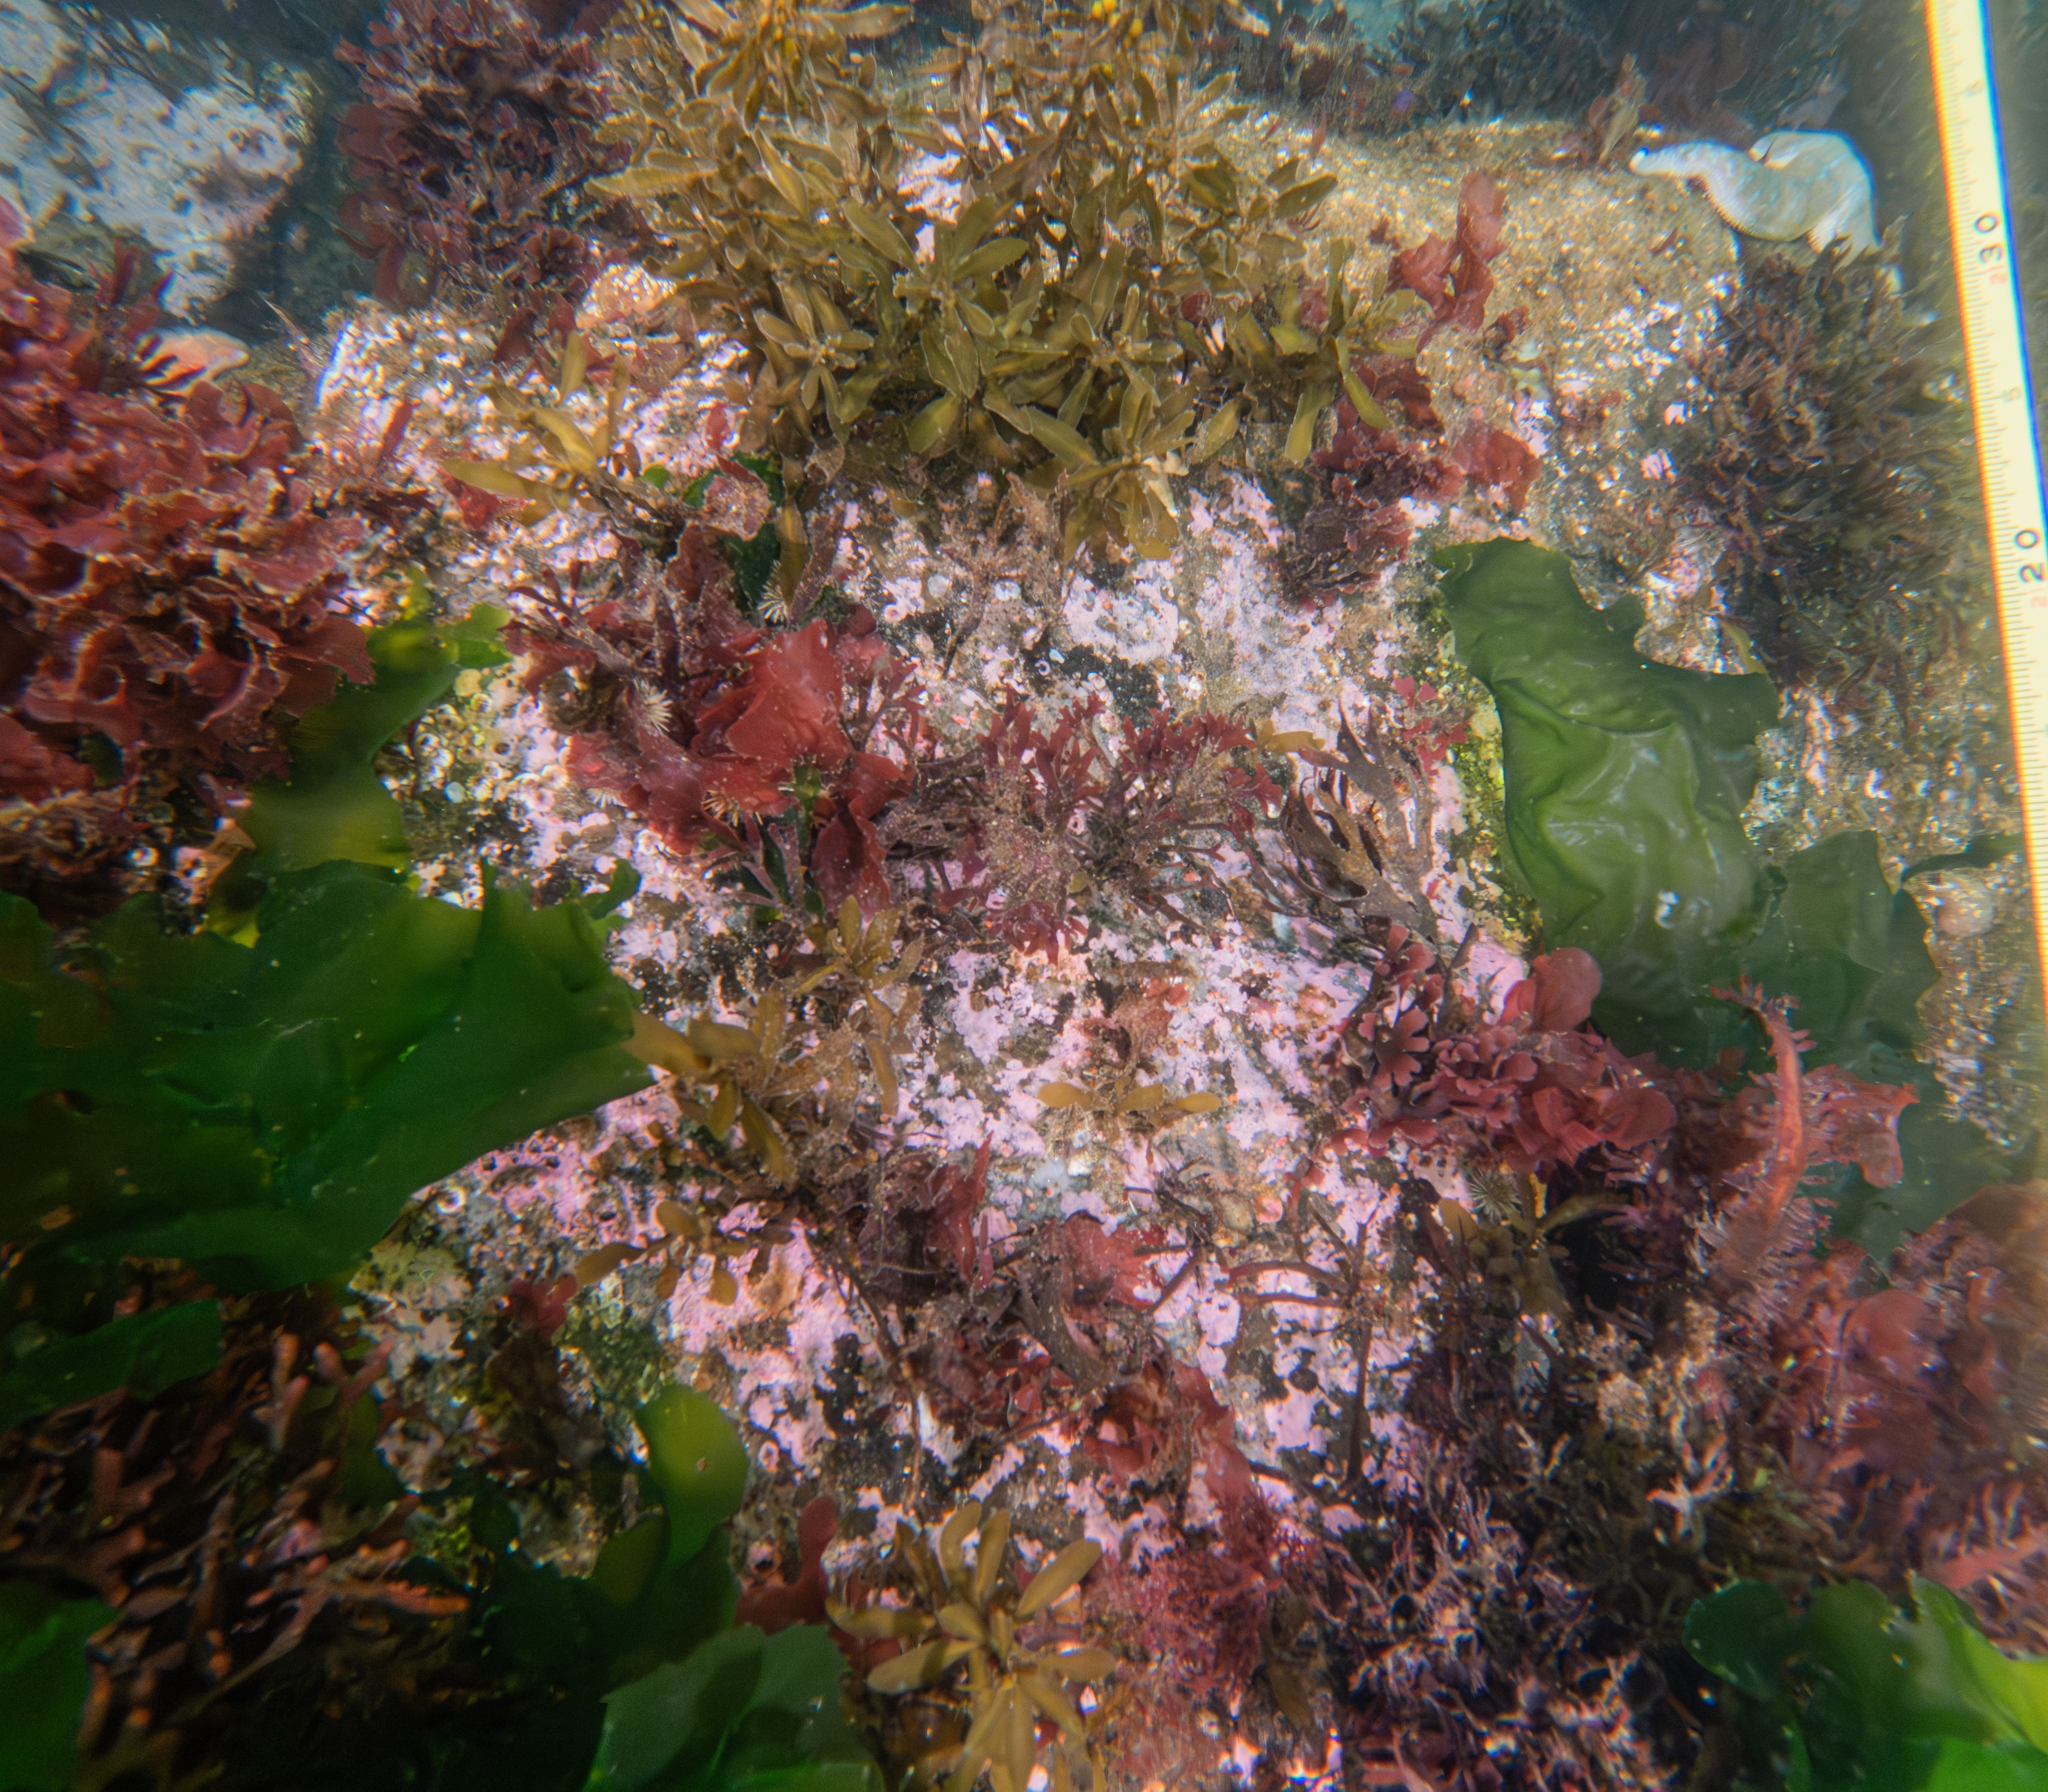
\includegraphics[width=0.326\textwidth]{EBM_shallow_2.jpg}%
\hspace{0.005\textwidth}%
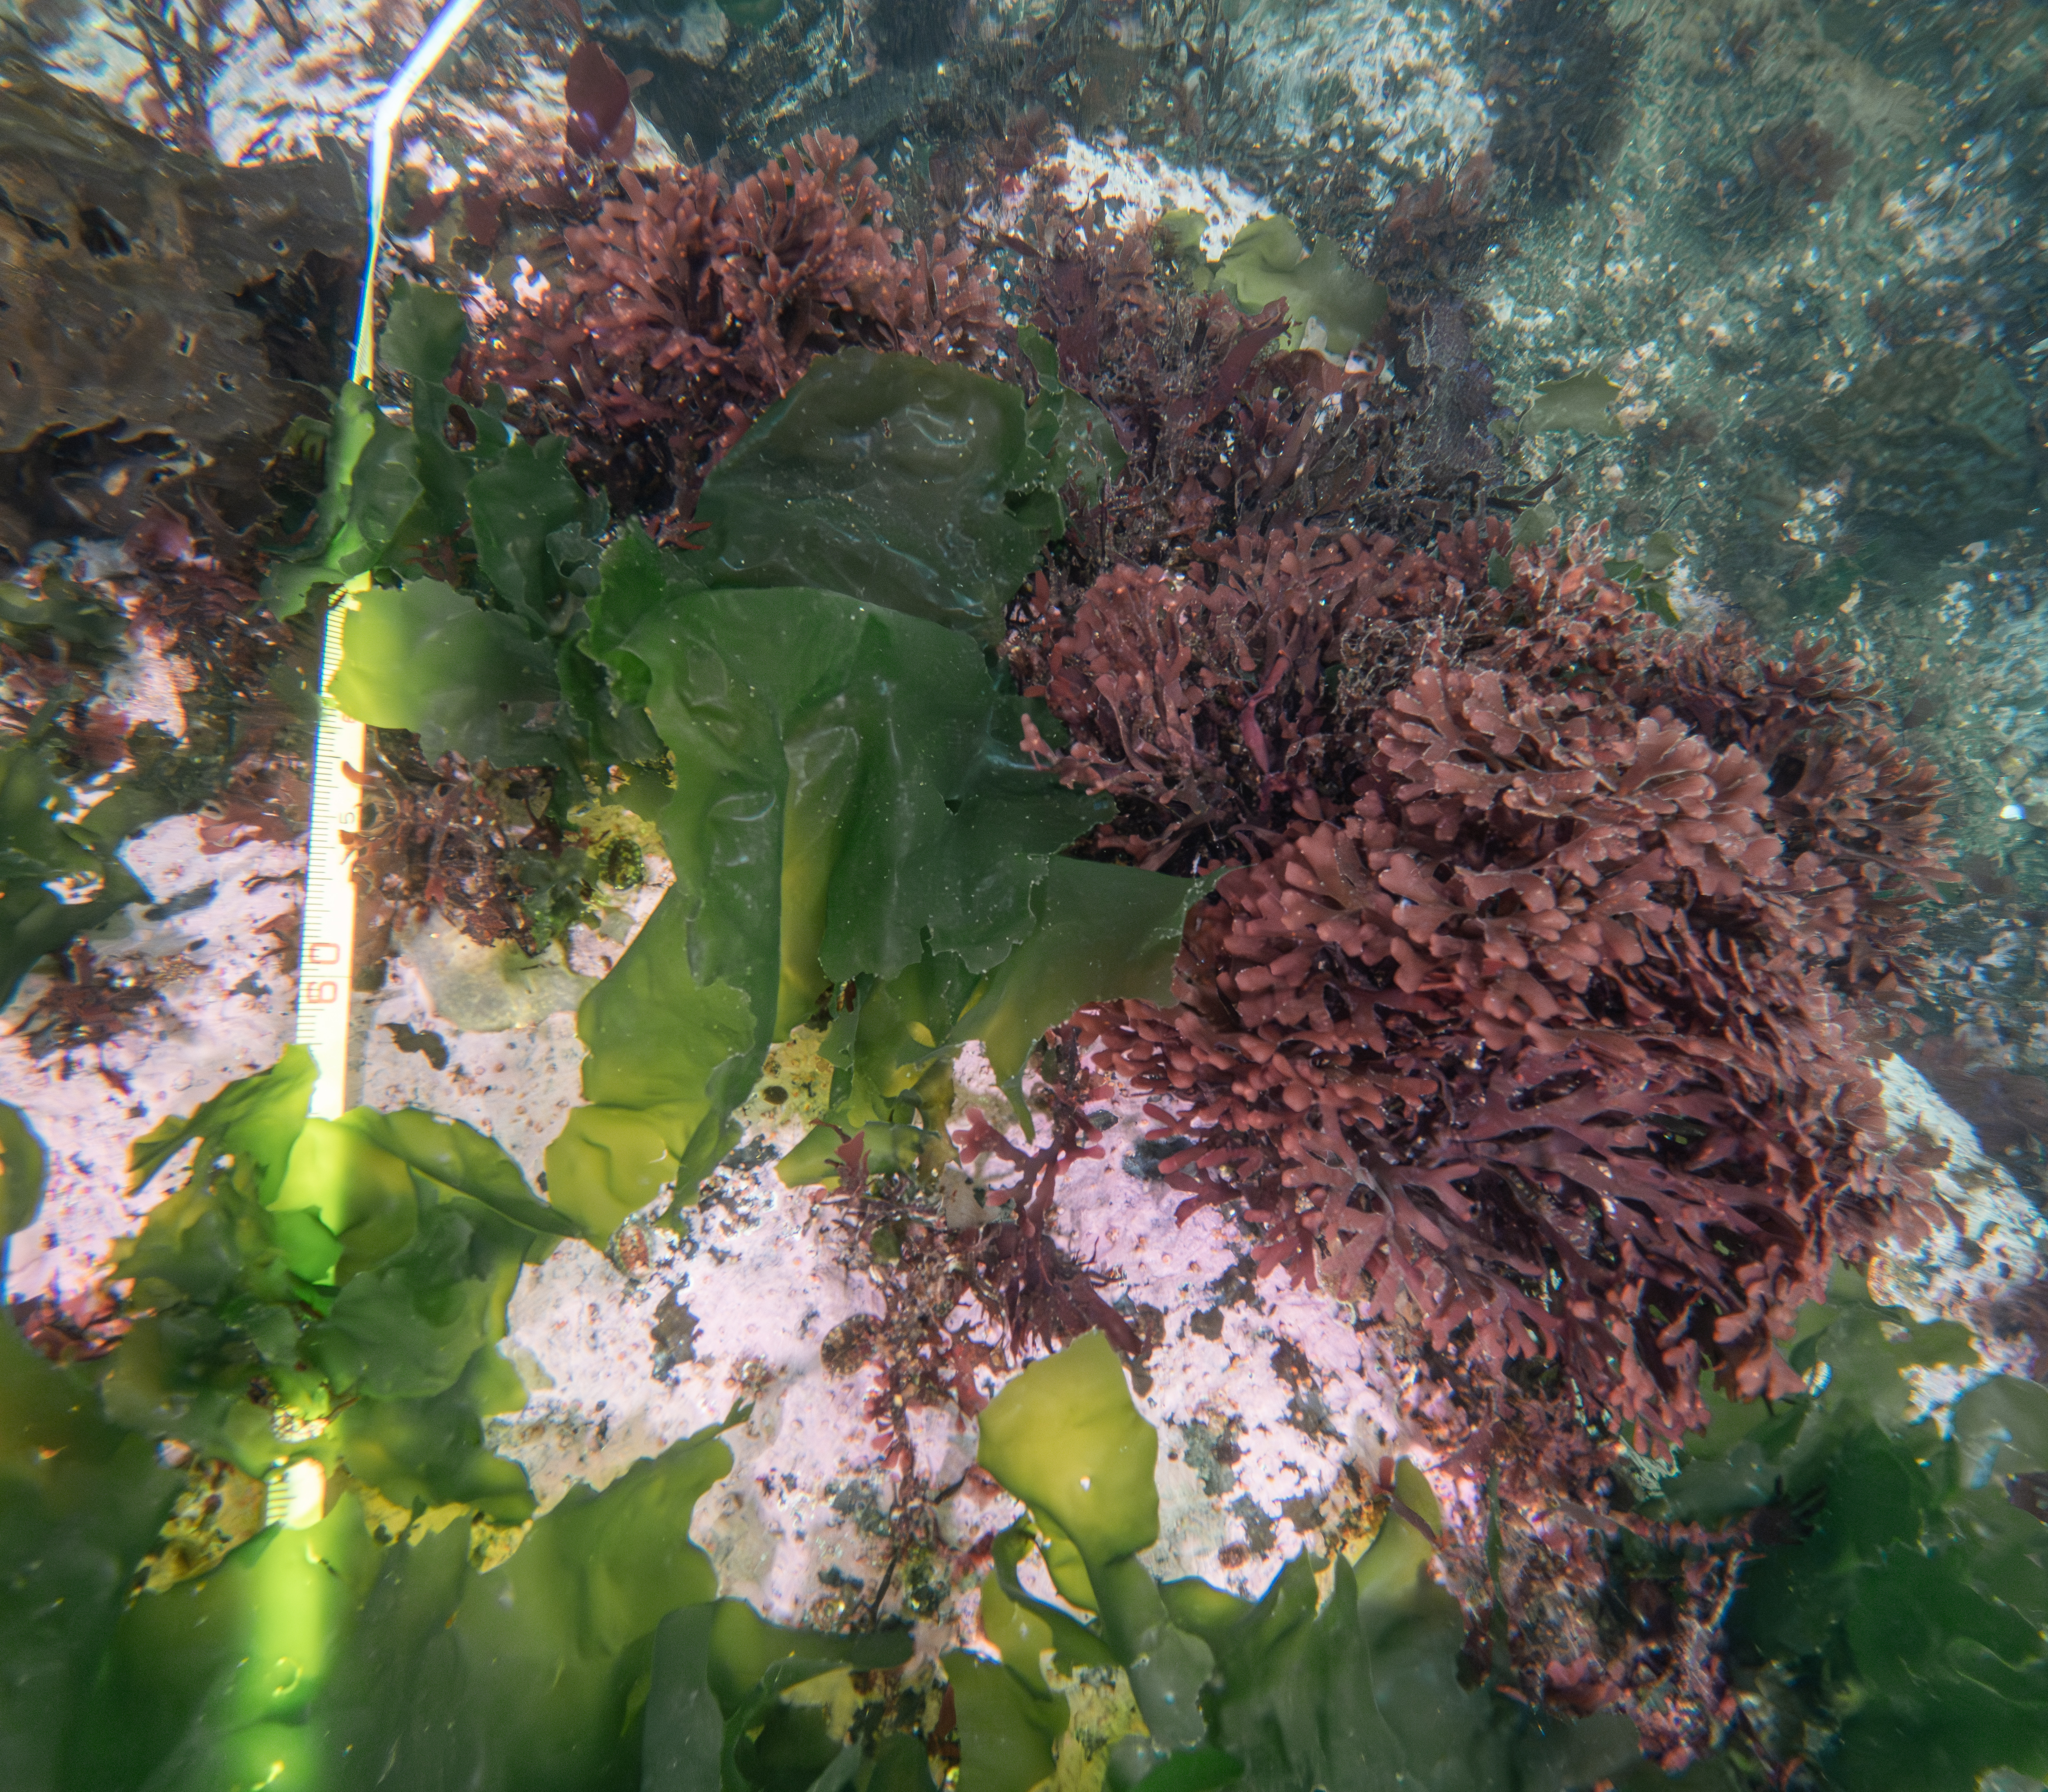
\includegraphics[width=0.326\textwidth]{EBM_shallow_3.jpg}\par
\vspace{0.005\textwidth}
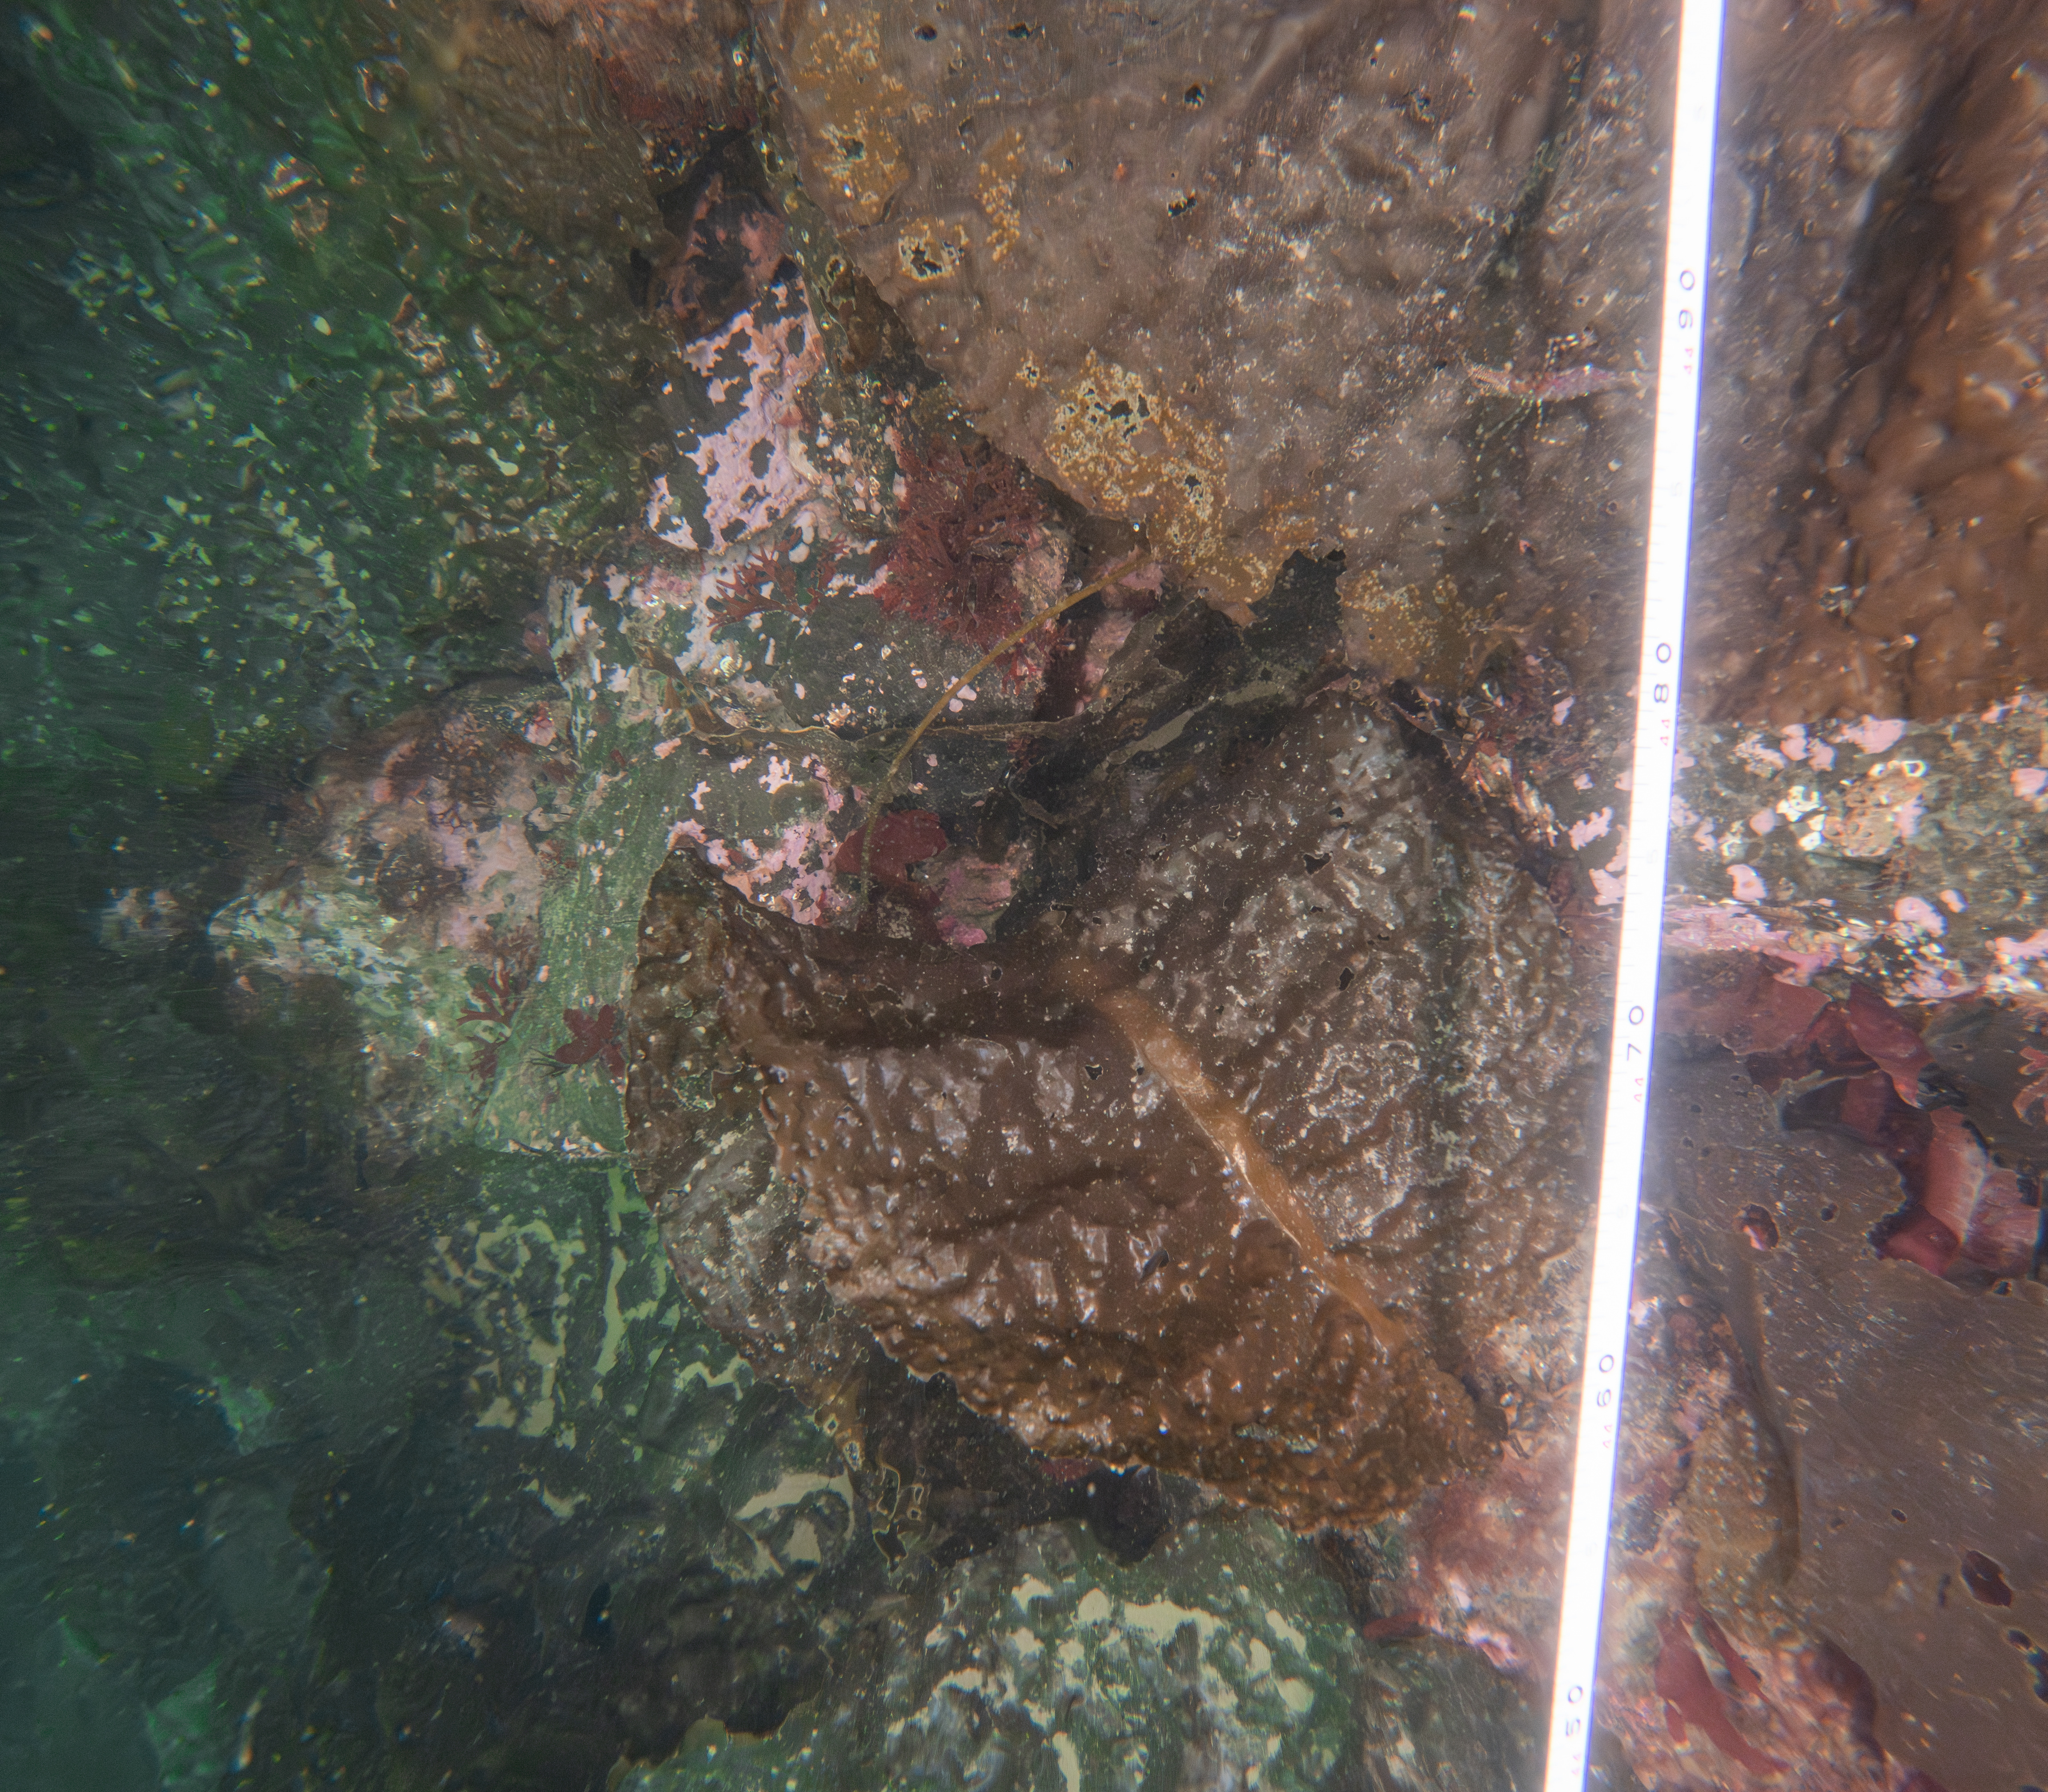
\includegraphics[width=0.326\textwidth]{EBM_deep_1.jpg}%
\hspace{0.005\textwidth}%
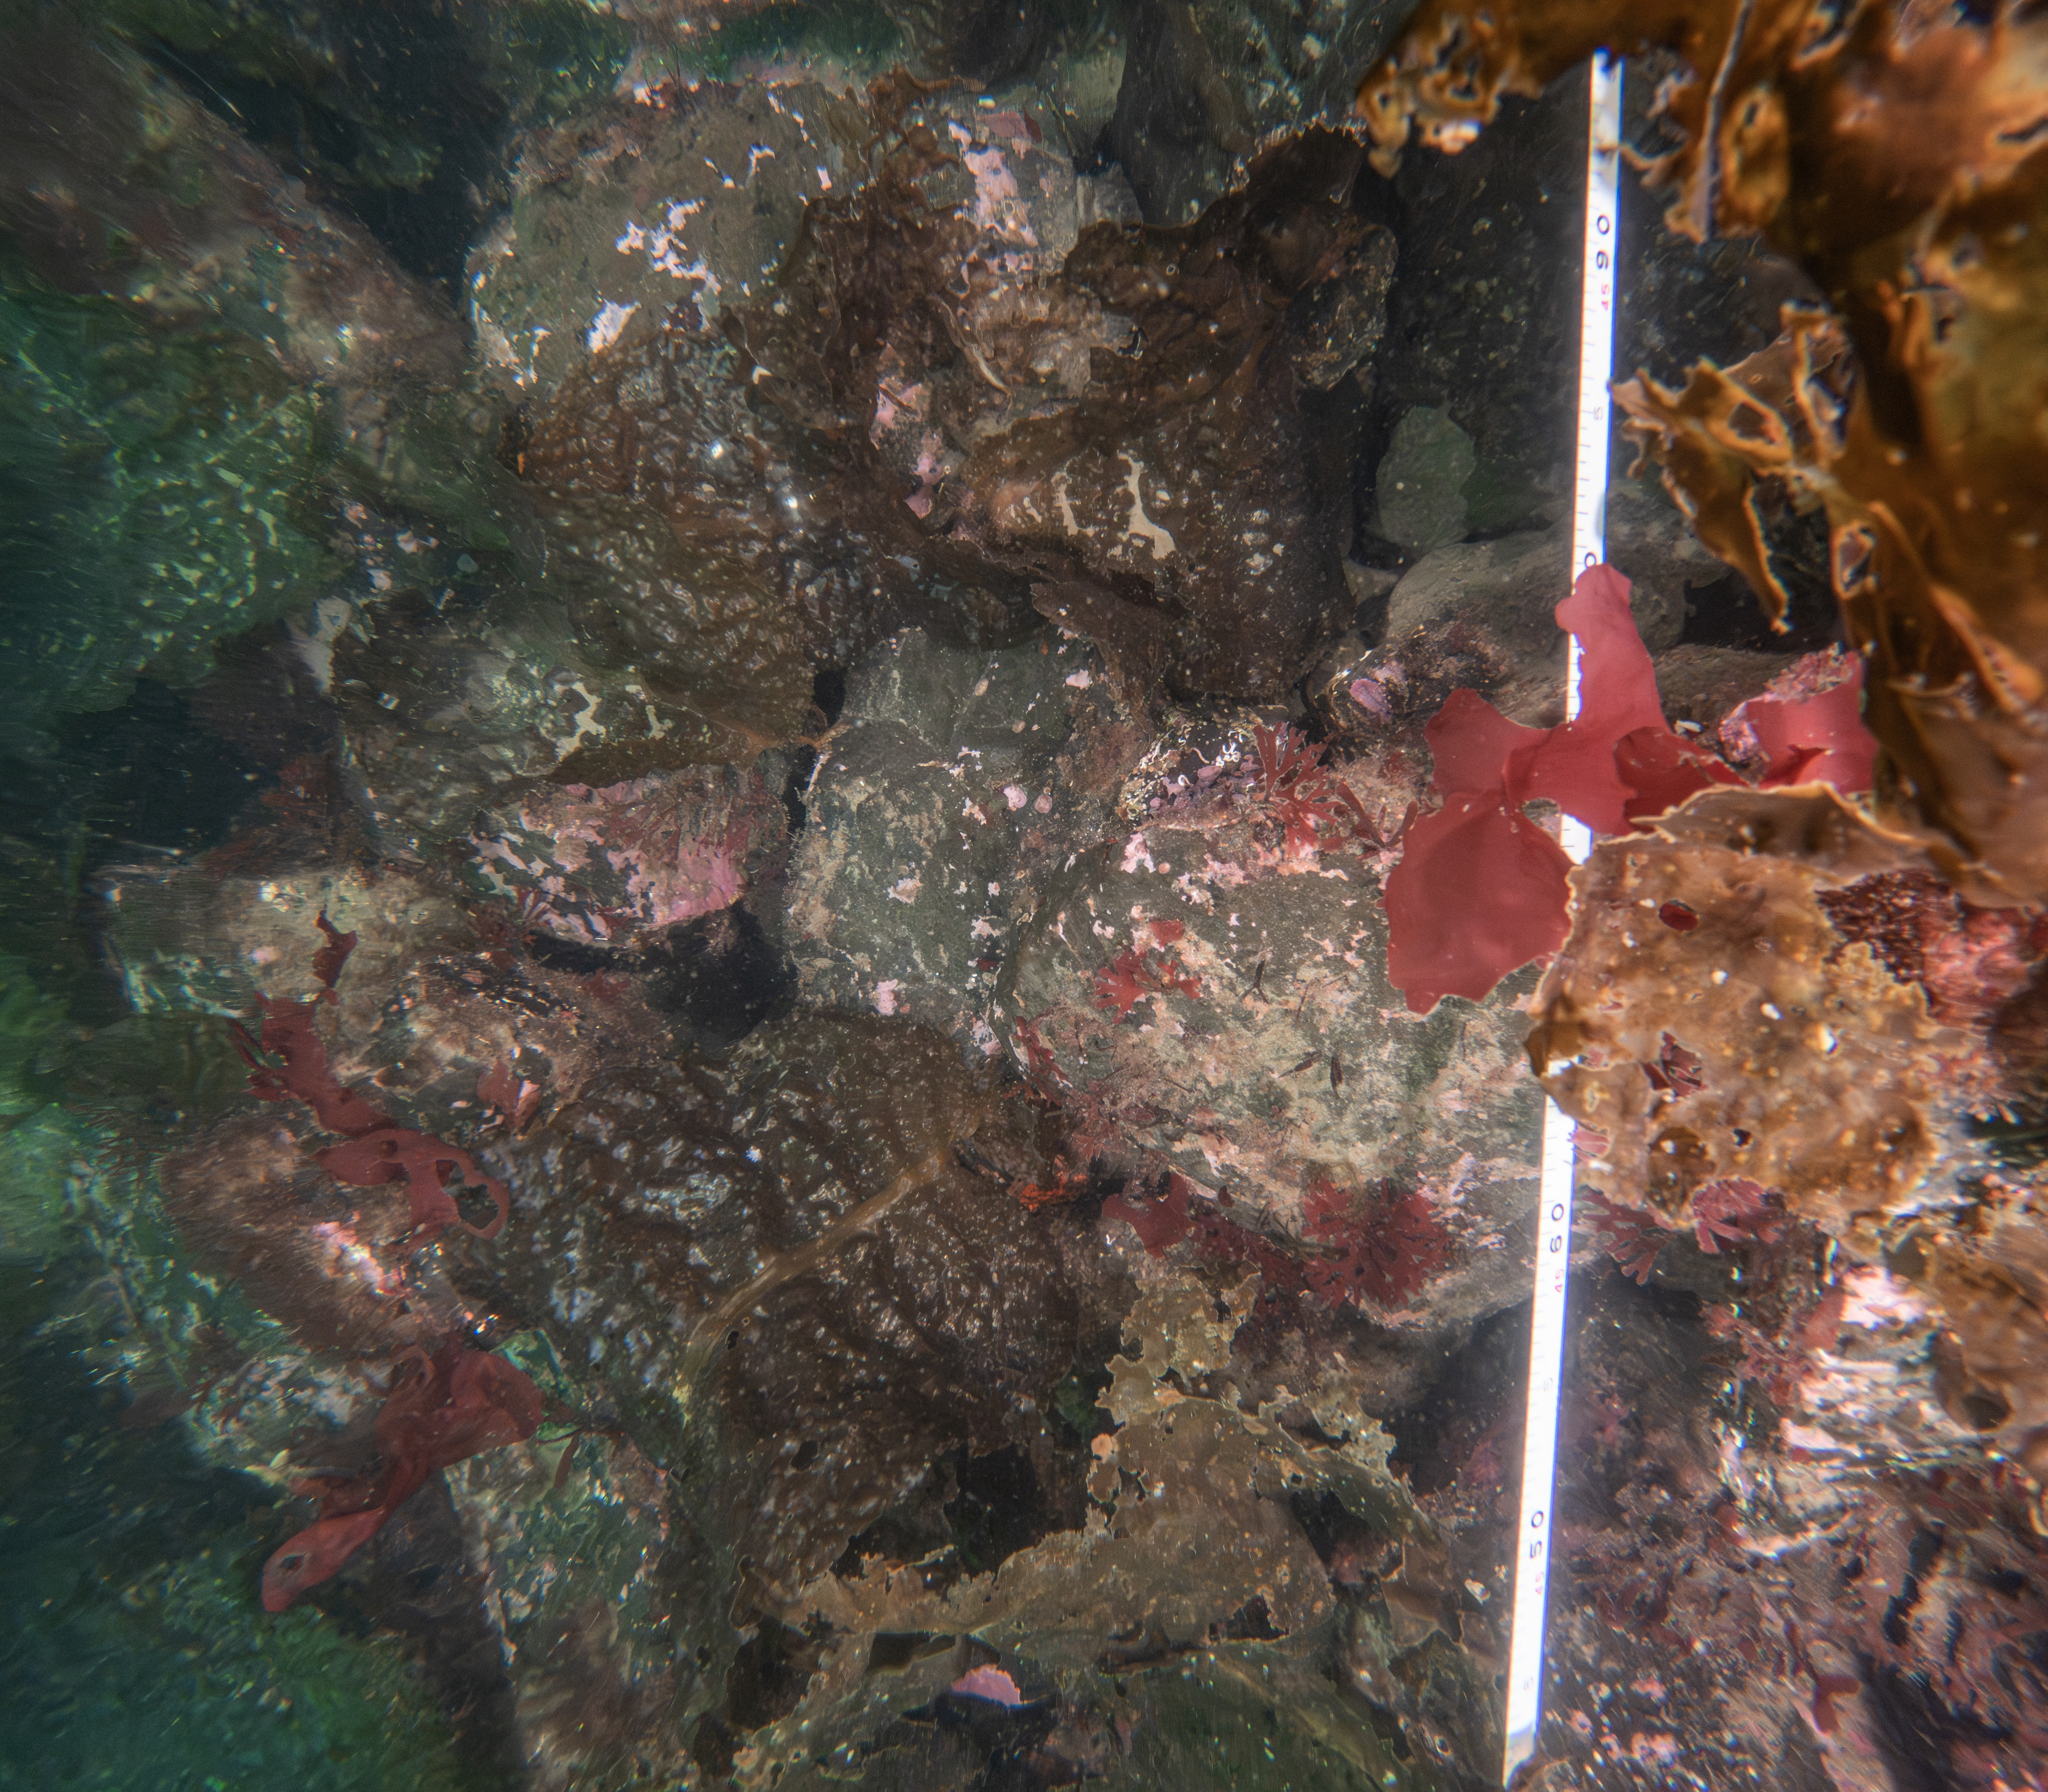
\includegraphics[width=0.326\textwidth]{EBM_deep_2.jpg}%
\hspace{0.005\textwidth}%
\includegraphics[width=0.326\textwidth]{EBM_deep_3.jpg}\par
\vspace{0.005\textwidth}
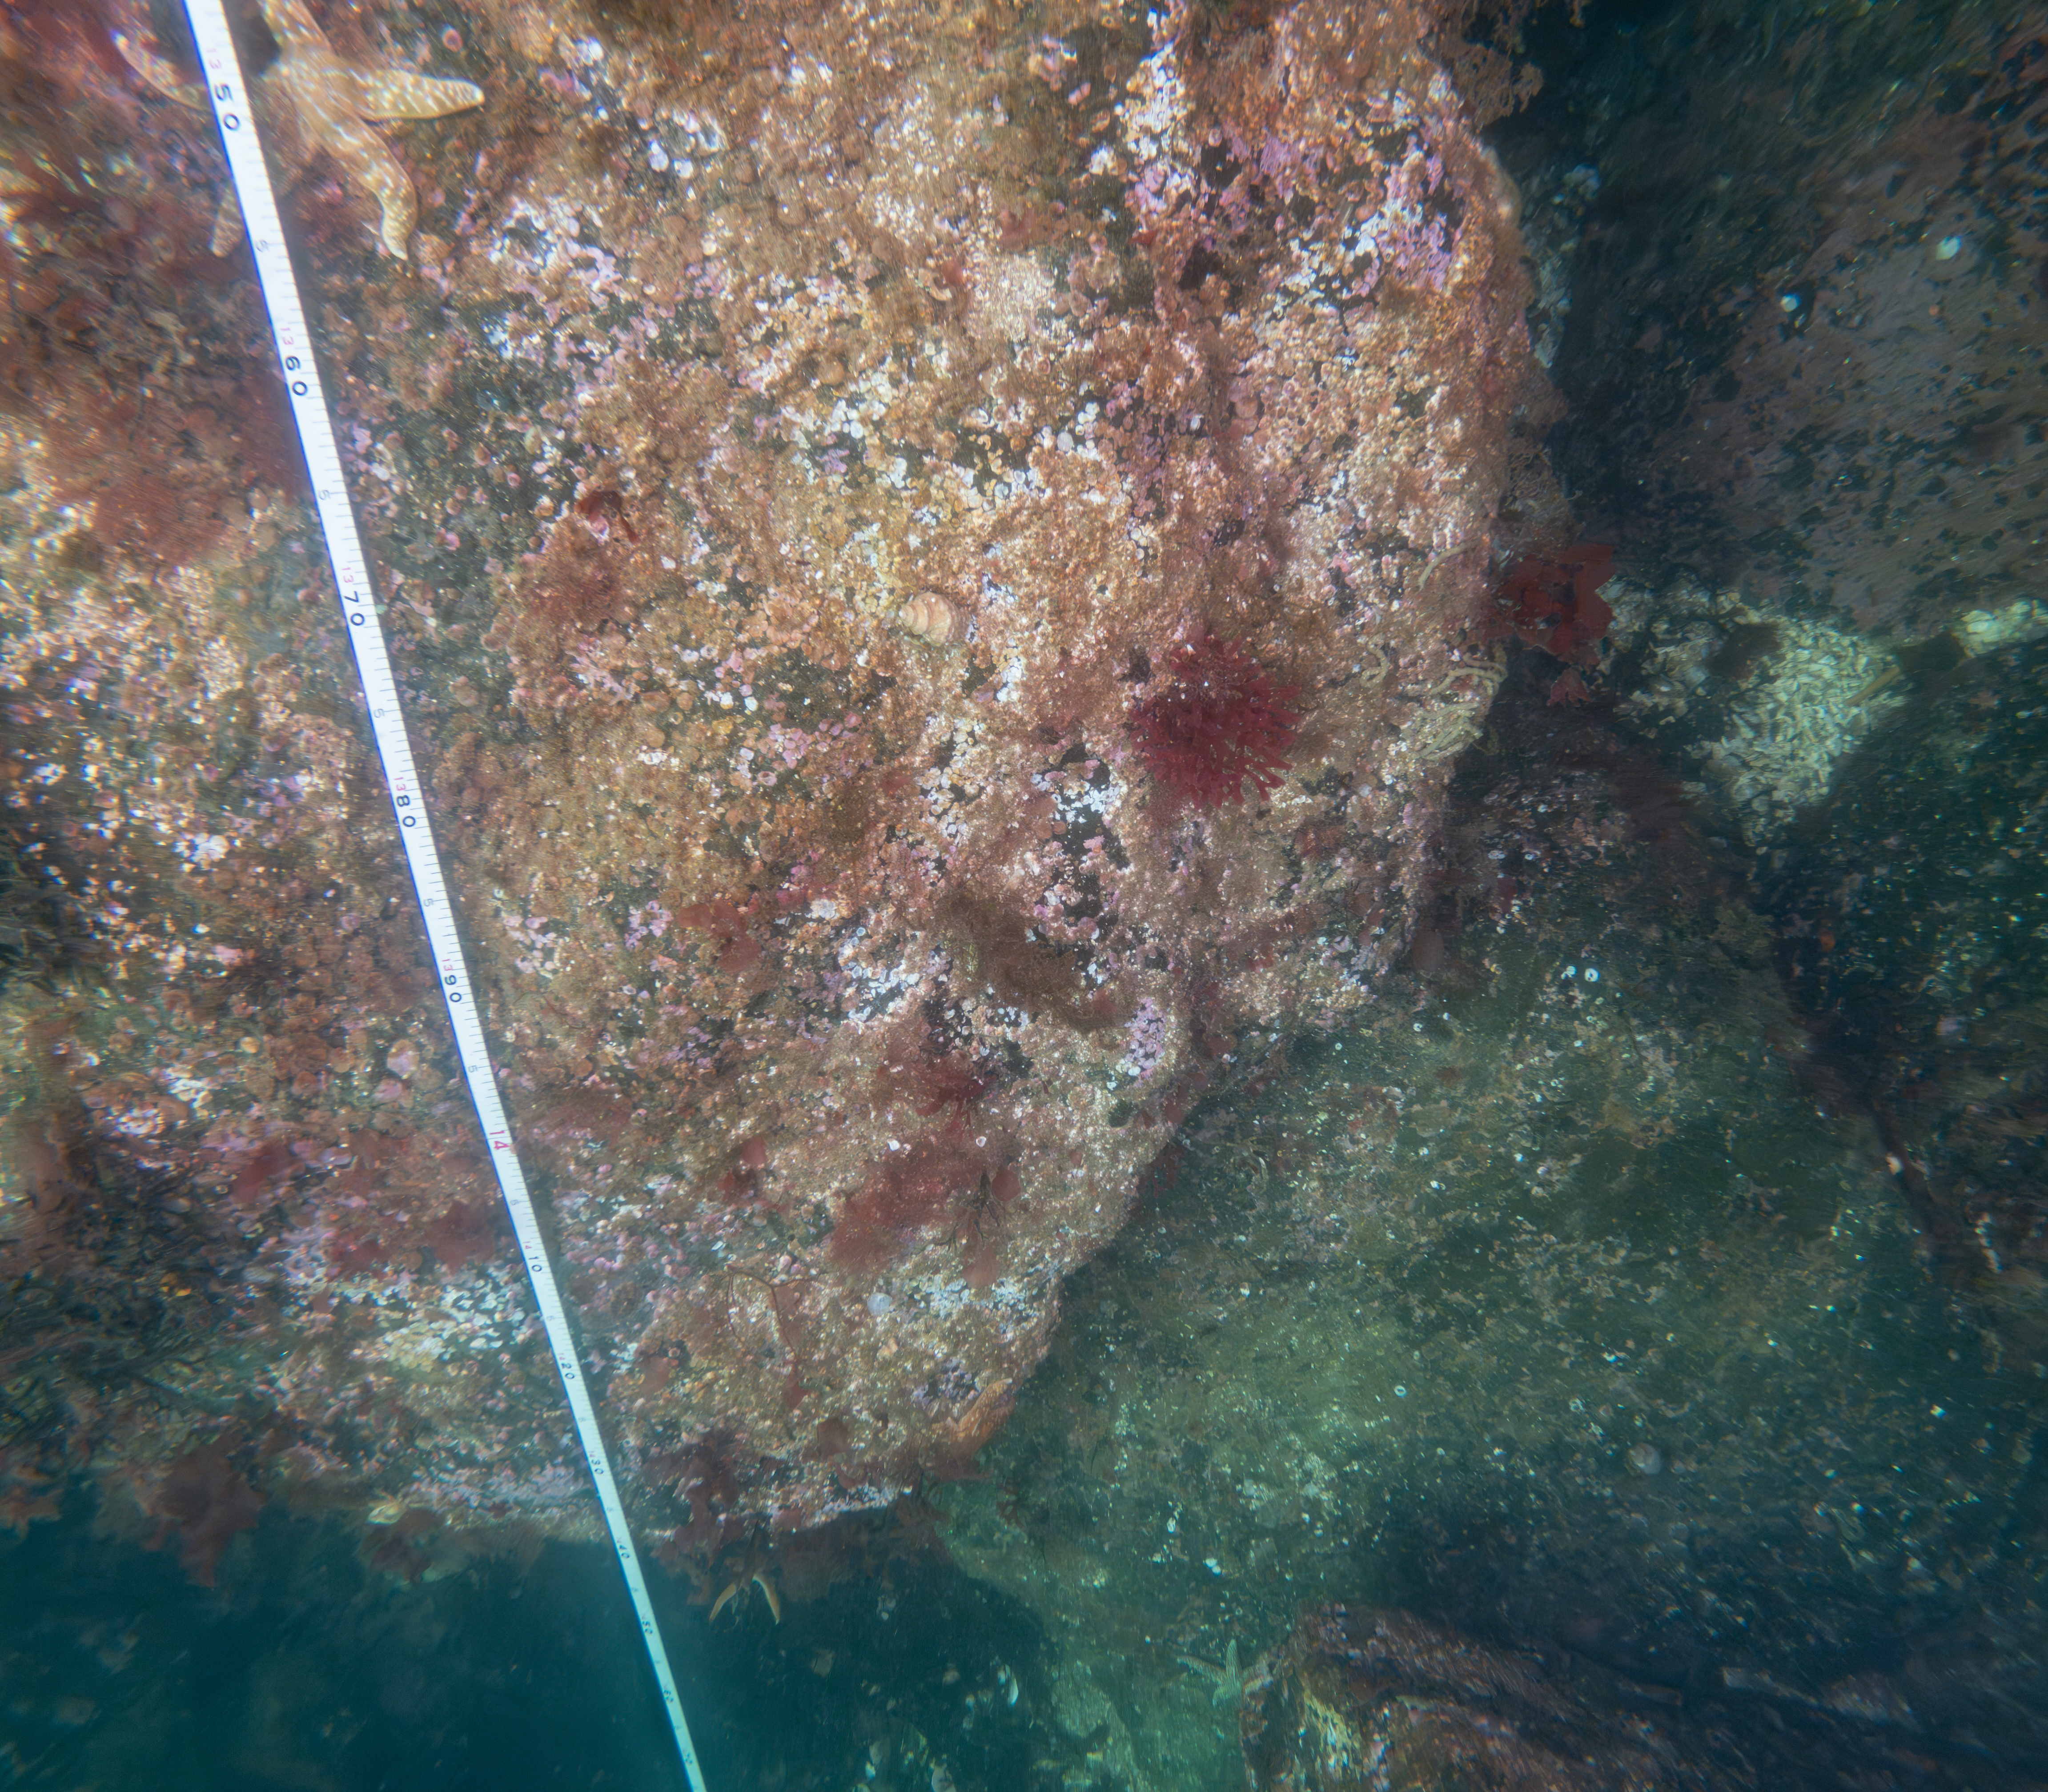
\includegraphics[width=0.326\textwidth]{EBM_winter_1.jpg}%
\hspace{0.005\textwidth}%
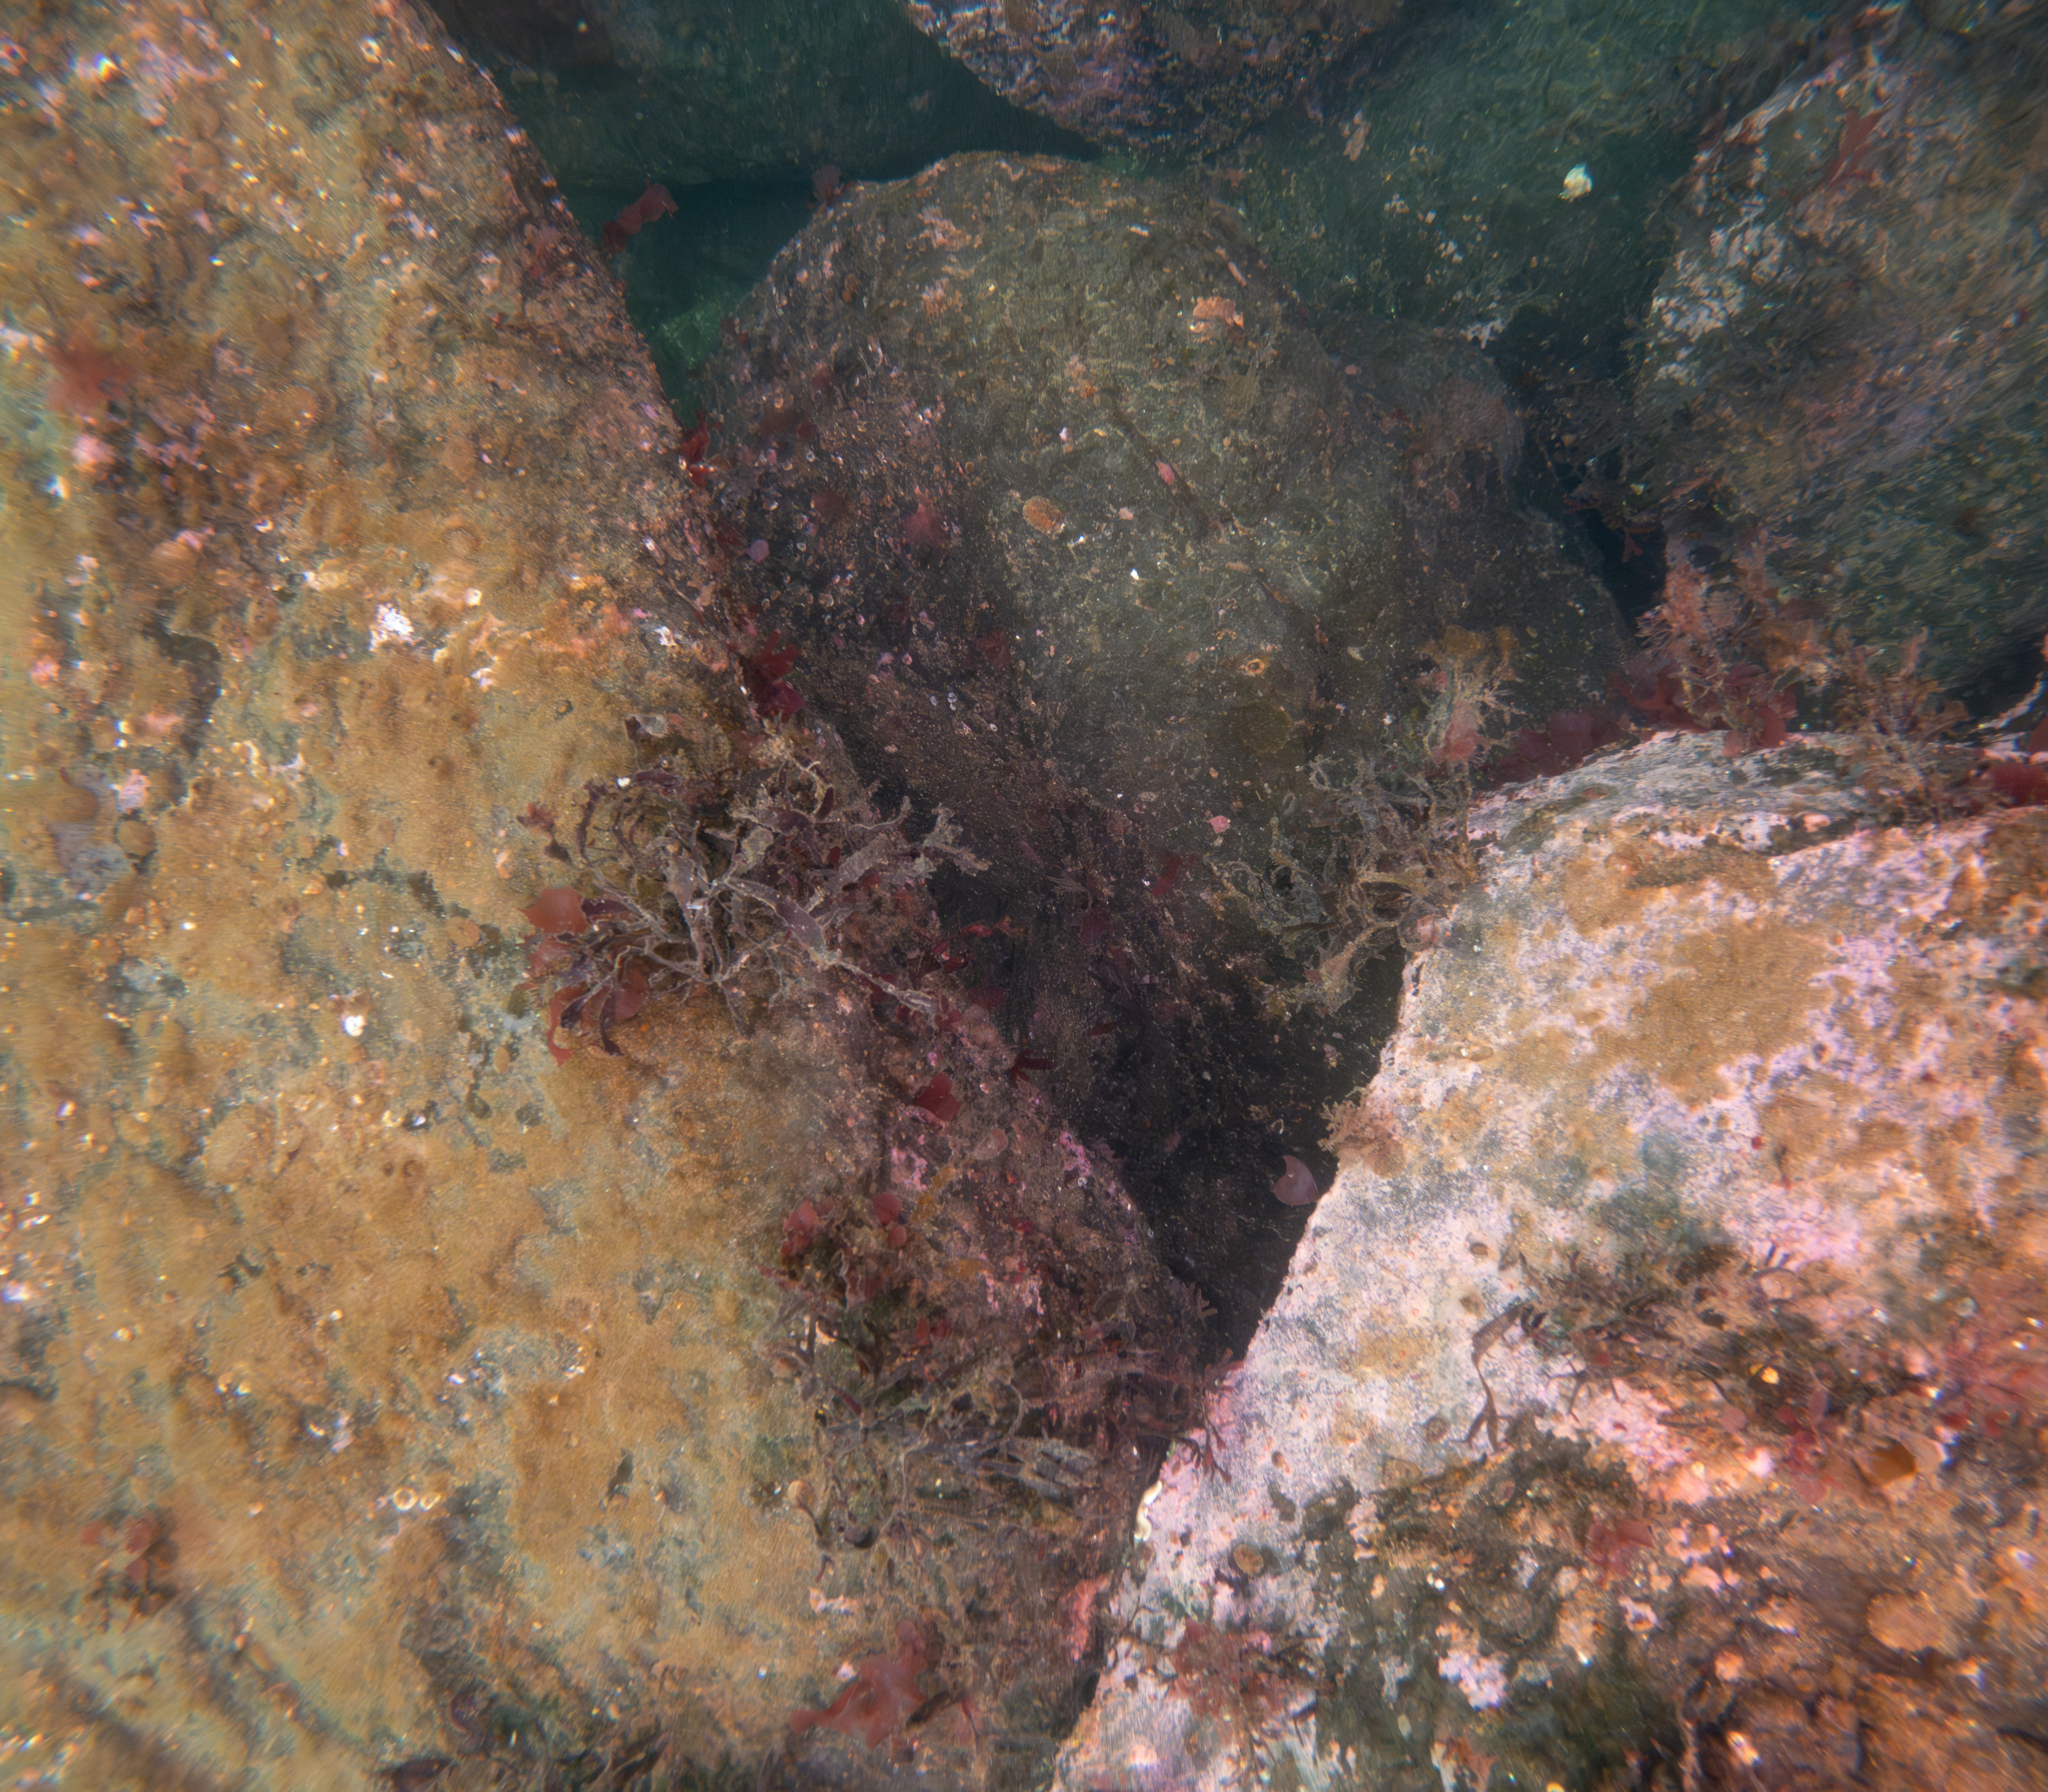
\includegraphics[width=0.326\textwidth]{EBM_winter_2.jpg}%
\hspace{0.005\textwidth}%
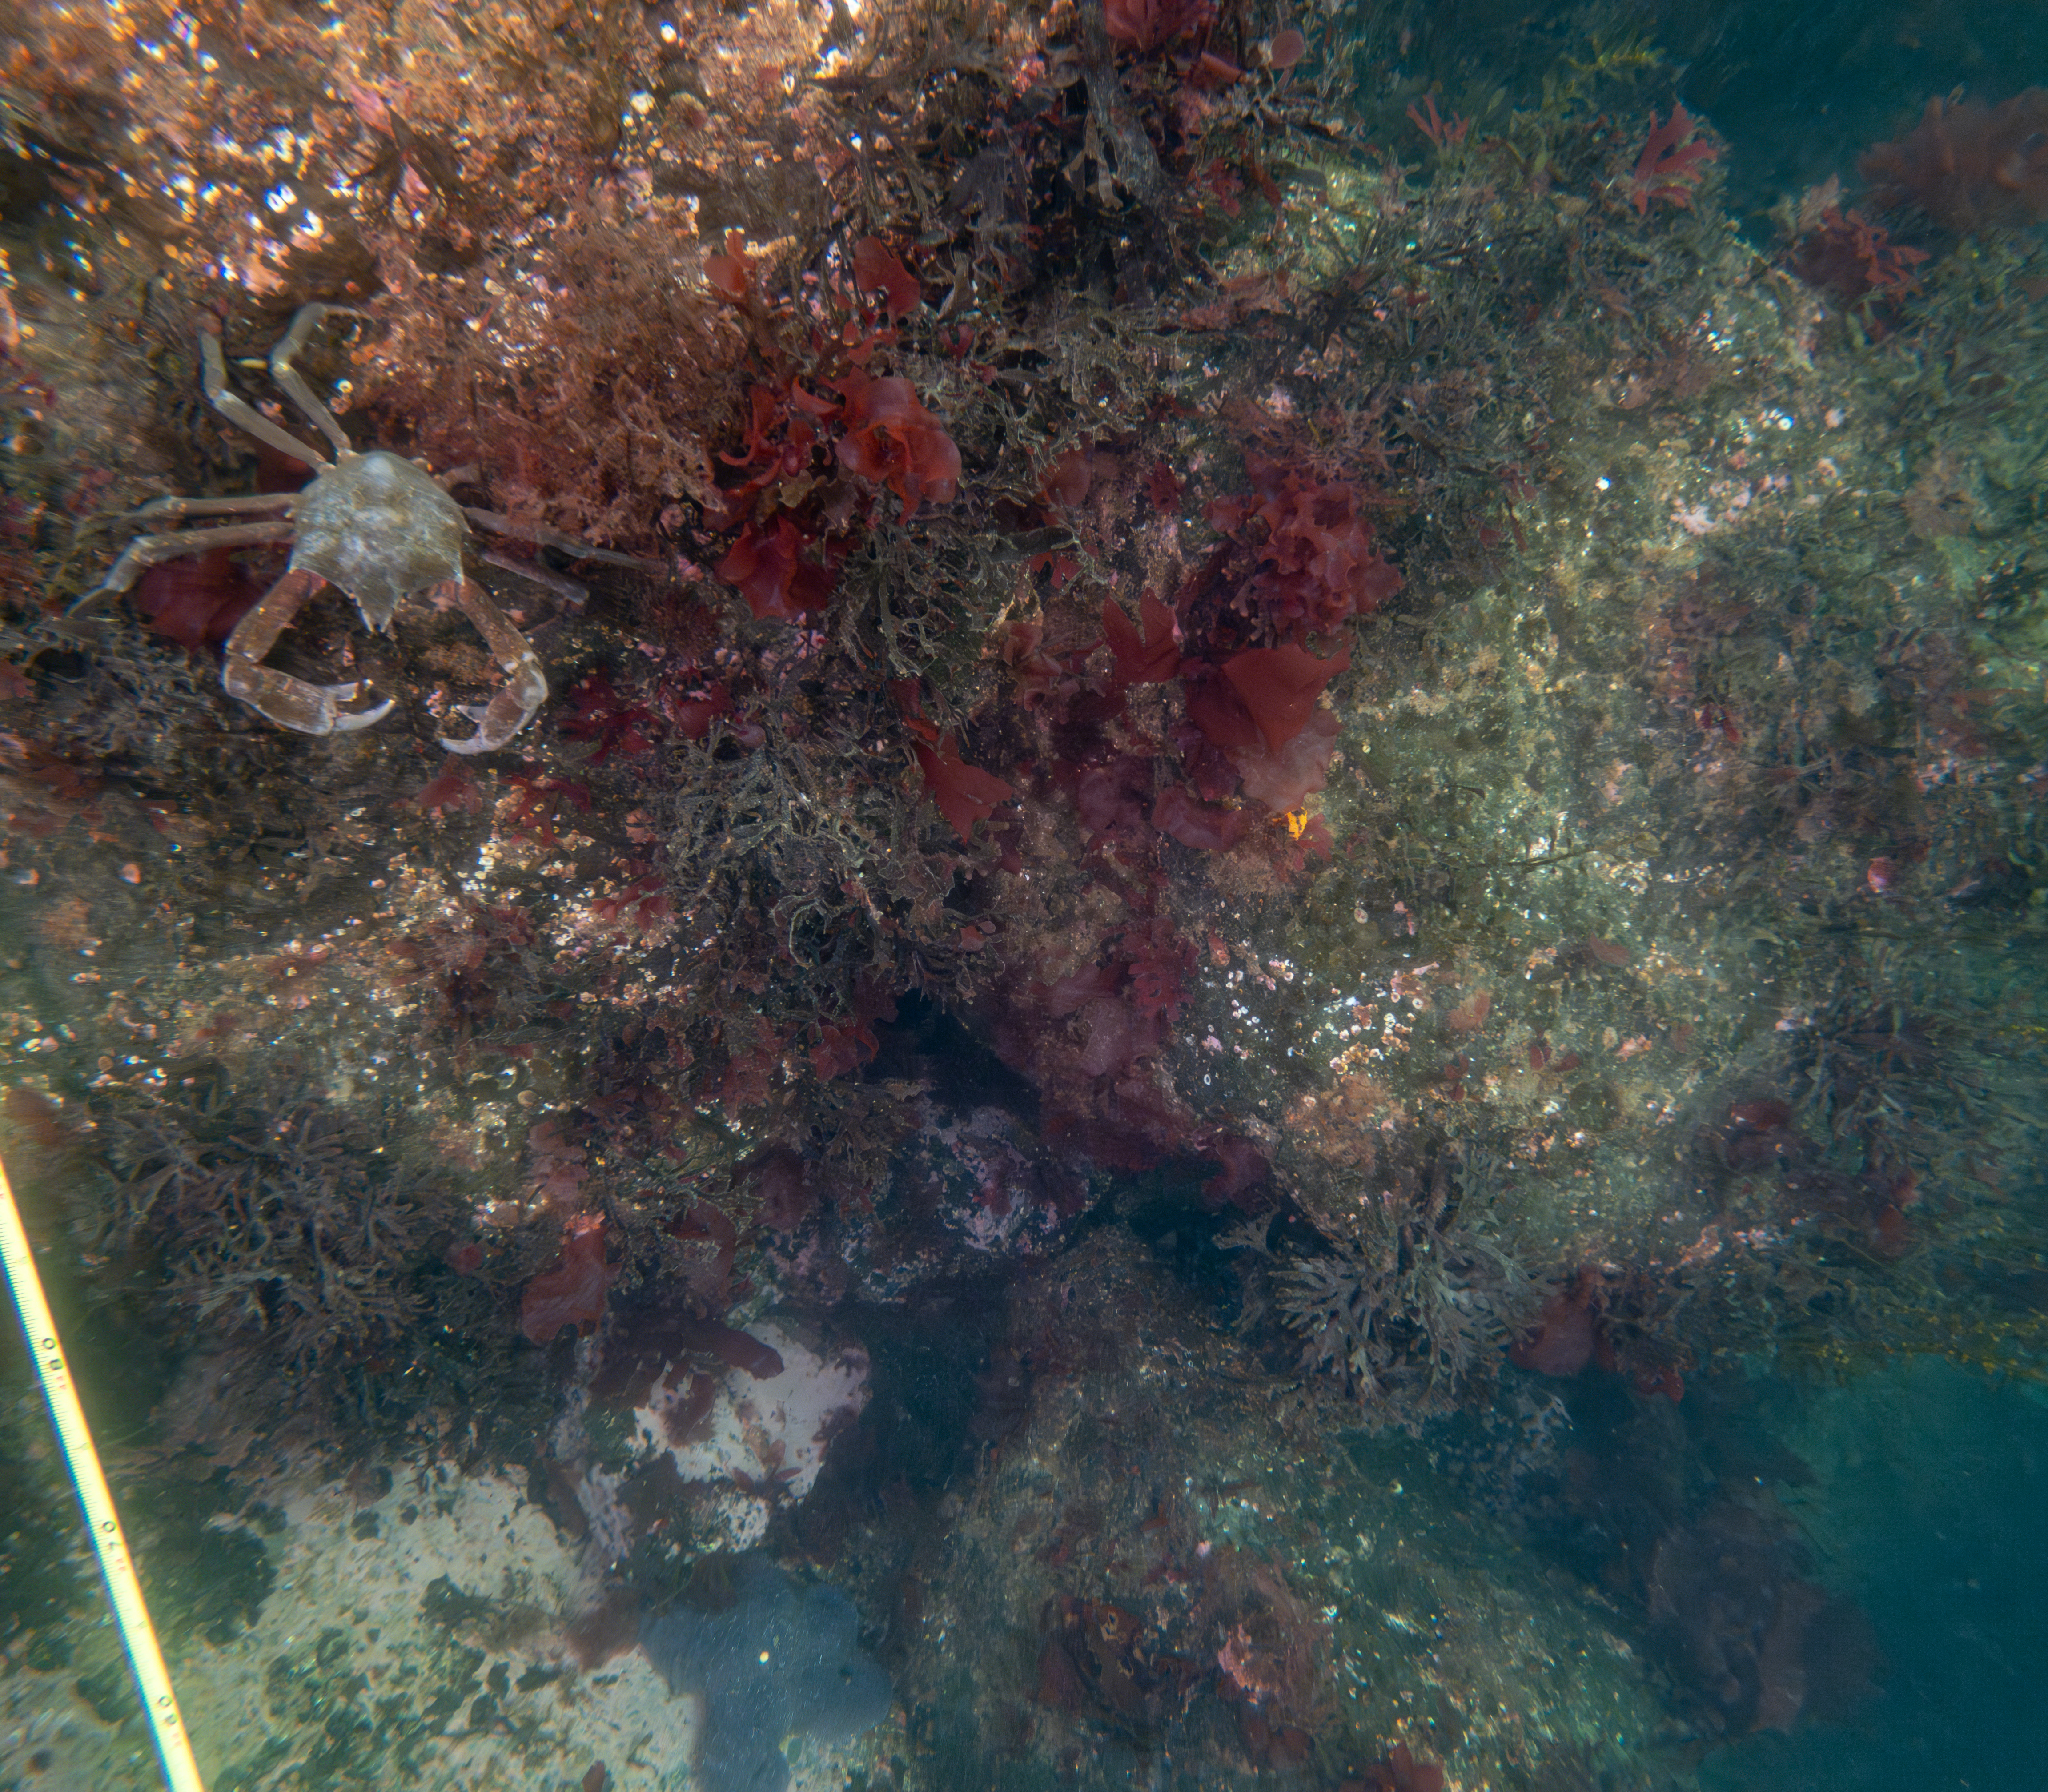
\includegraphics[width=0.326\textwidth]{EBM_winter_3.jpg}
\caption{
Nine example ROV survey images from Elliott Bay Marina breakwater. 
Row 1 depicts three images from the shallow transects ($5~m$ depth) in the 
summer of 2024;
Row 2 depicts three images from the deep transects ($10~m$ depth) in the summer 
of 2024;
Row 3 depicts three images from the winter of 2025 (both depths).
Elliott Bay Marina breakwater consists of hard substrate comprised of
breakwater riprap boulder/reef structure.
Sieve kelp (\textit{Agarum clathratum}) is the predominant kelp found at 
this site. 
}
\label{fig:EBM}
\end{figure}
\vfil
}

\clearpage

\vbox to \textheight{%
\vfil
\begin{figure}[H]
\centering
\begin{subfigure}[t]{0.48\textwidth}
\centering
\textbf{(a)}\par
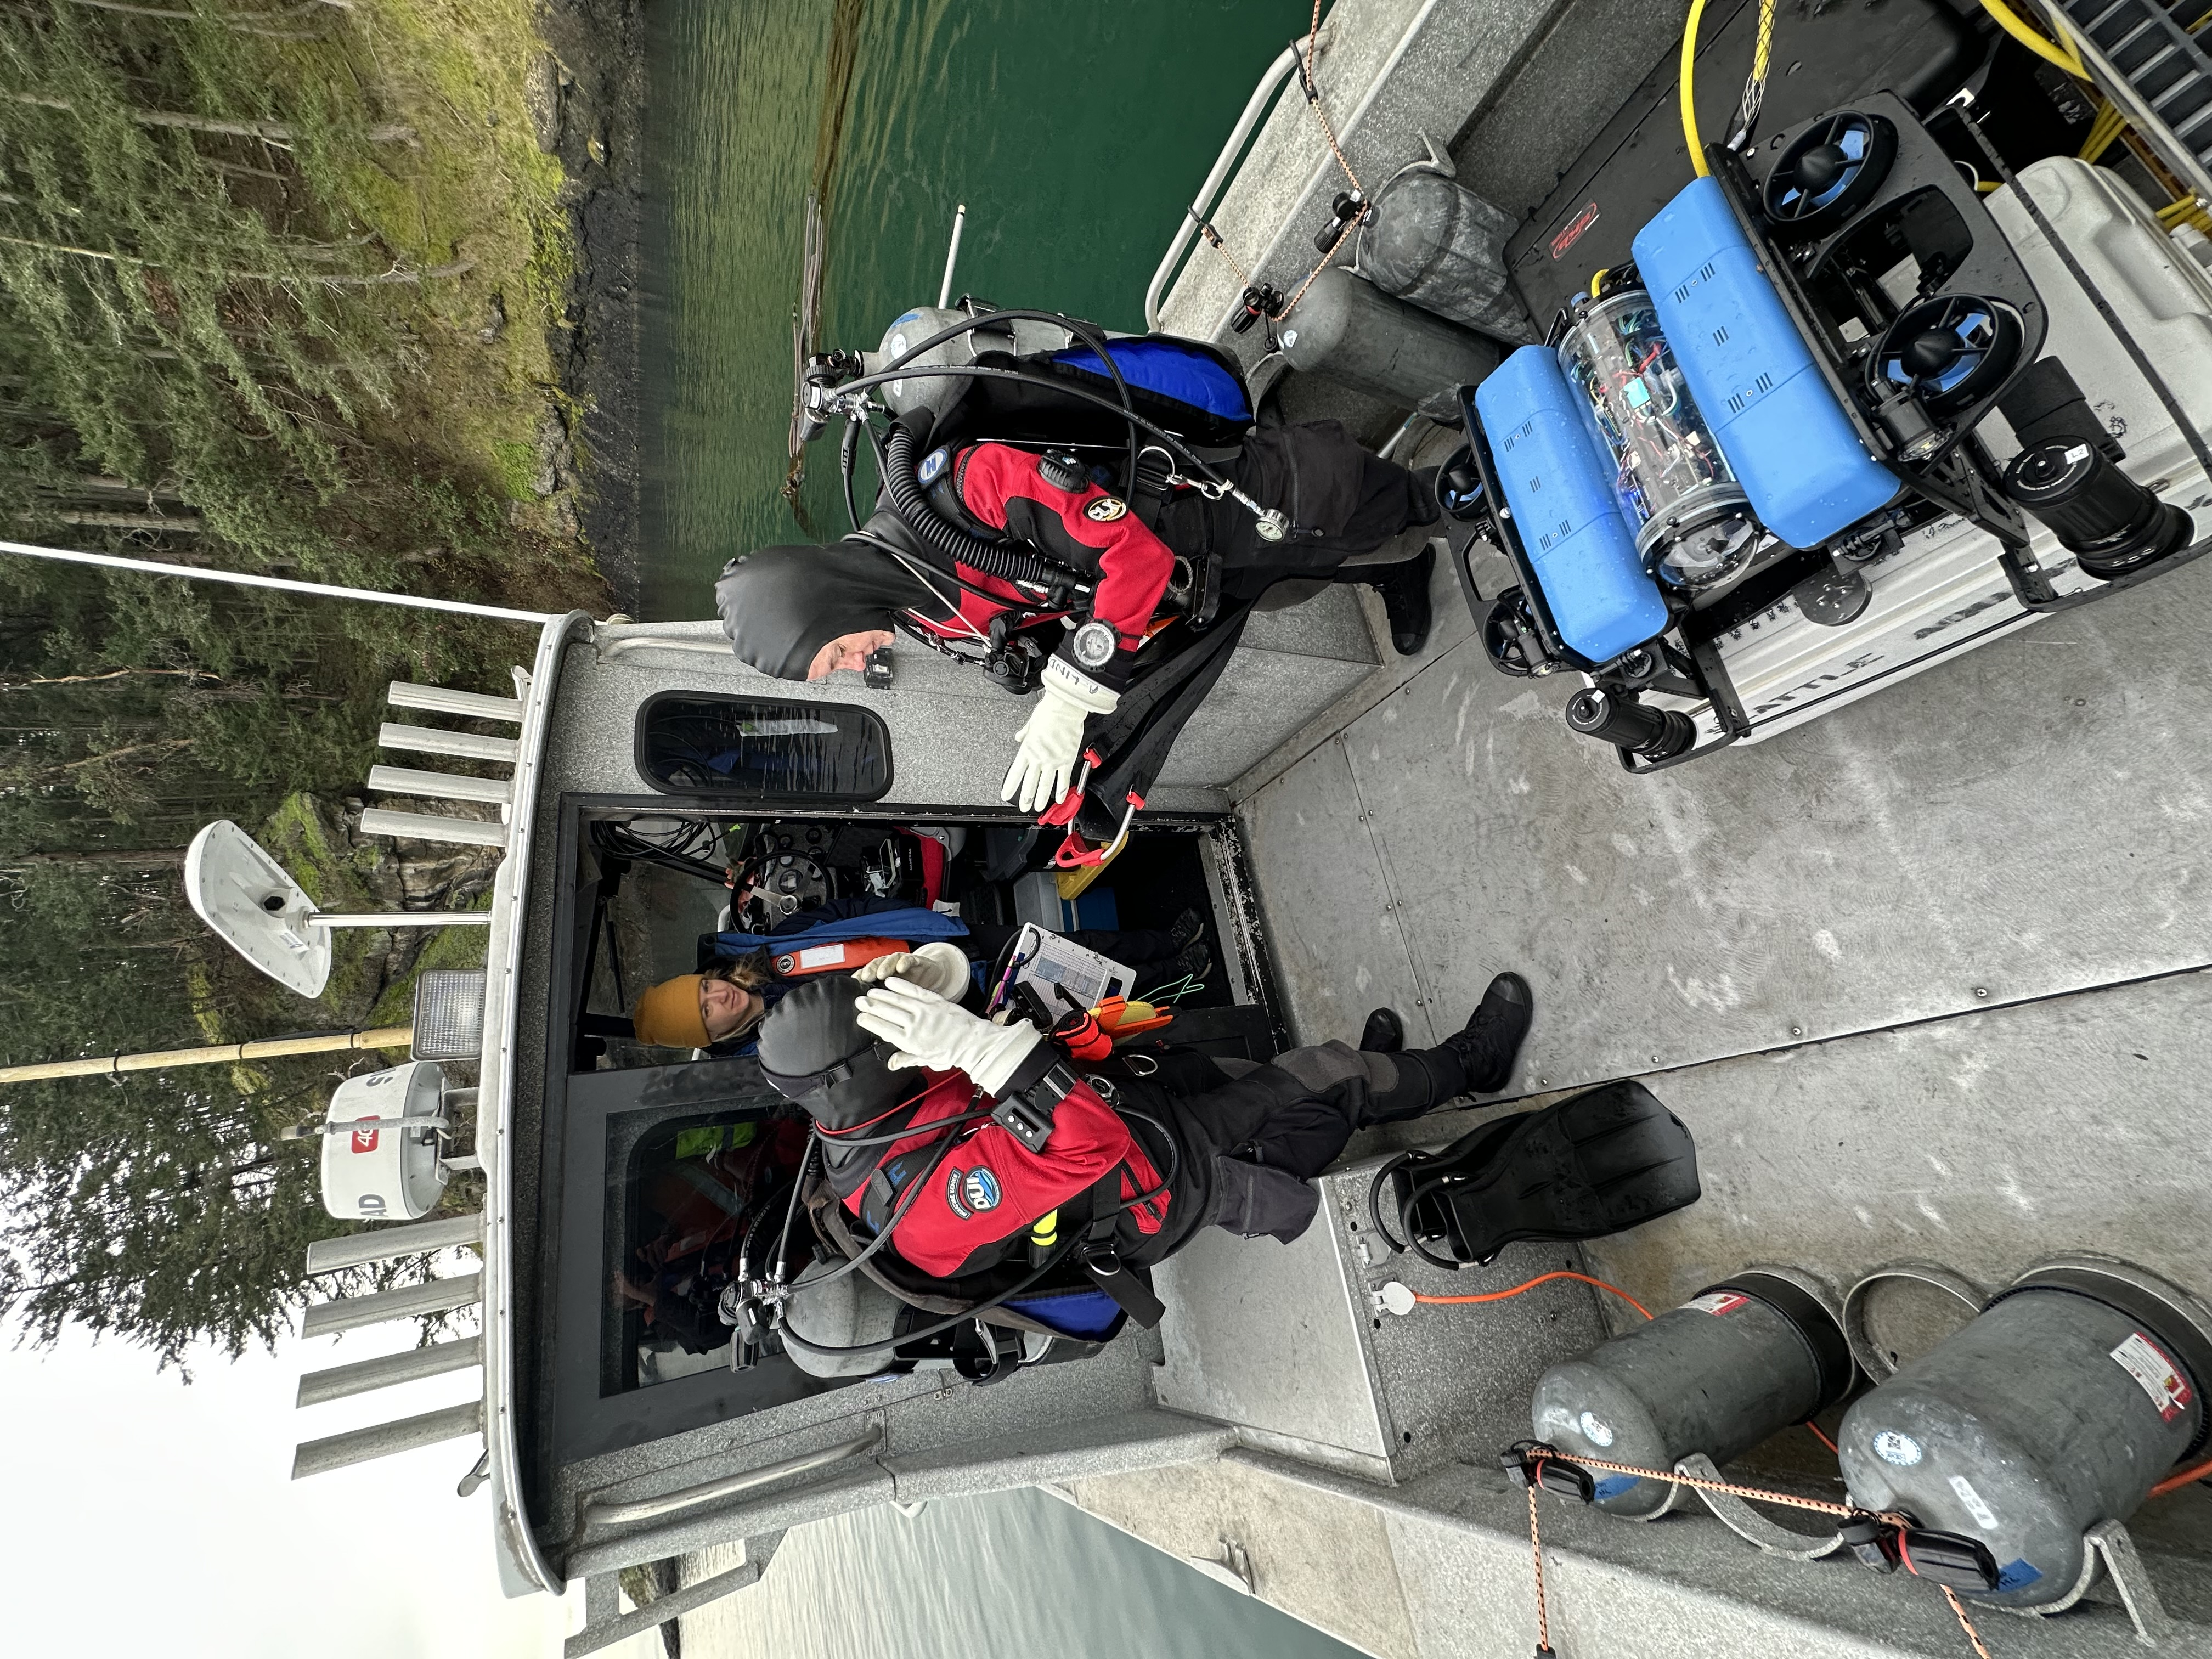
\includegraphics[angle=-90,origin=c,width=\linewidth]{field_methods_1.jpg}
\end{subfigure}
\hspace{0.01\textwidth}
\begin{subfigure}[t]{0.48\textwidth}
\centering
\textbf{(b)}\par
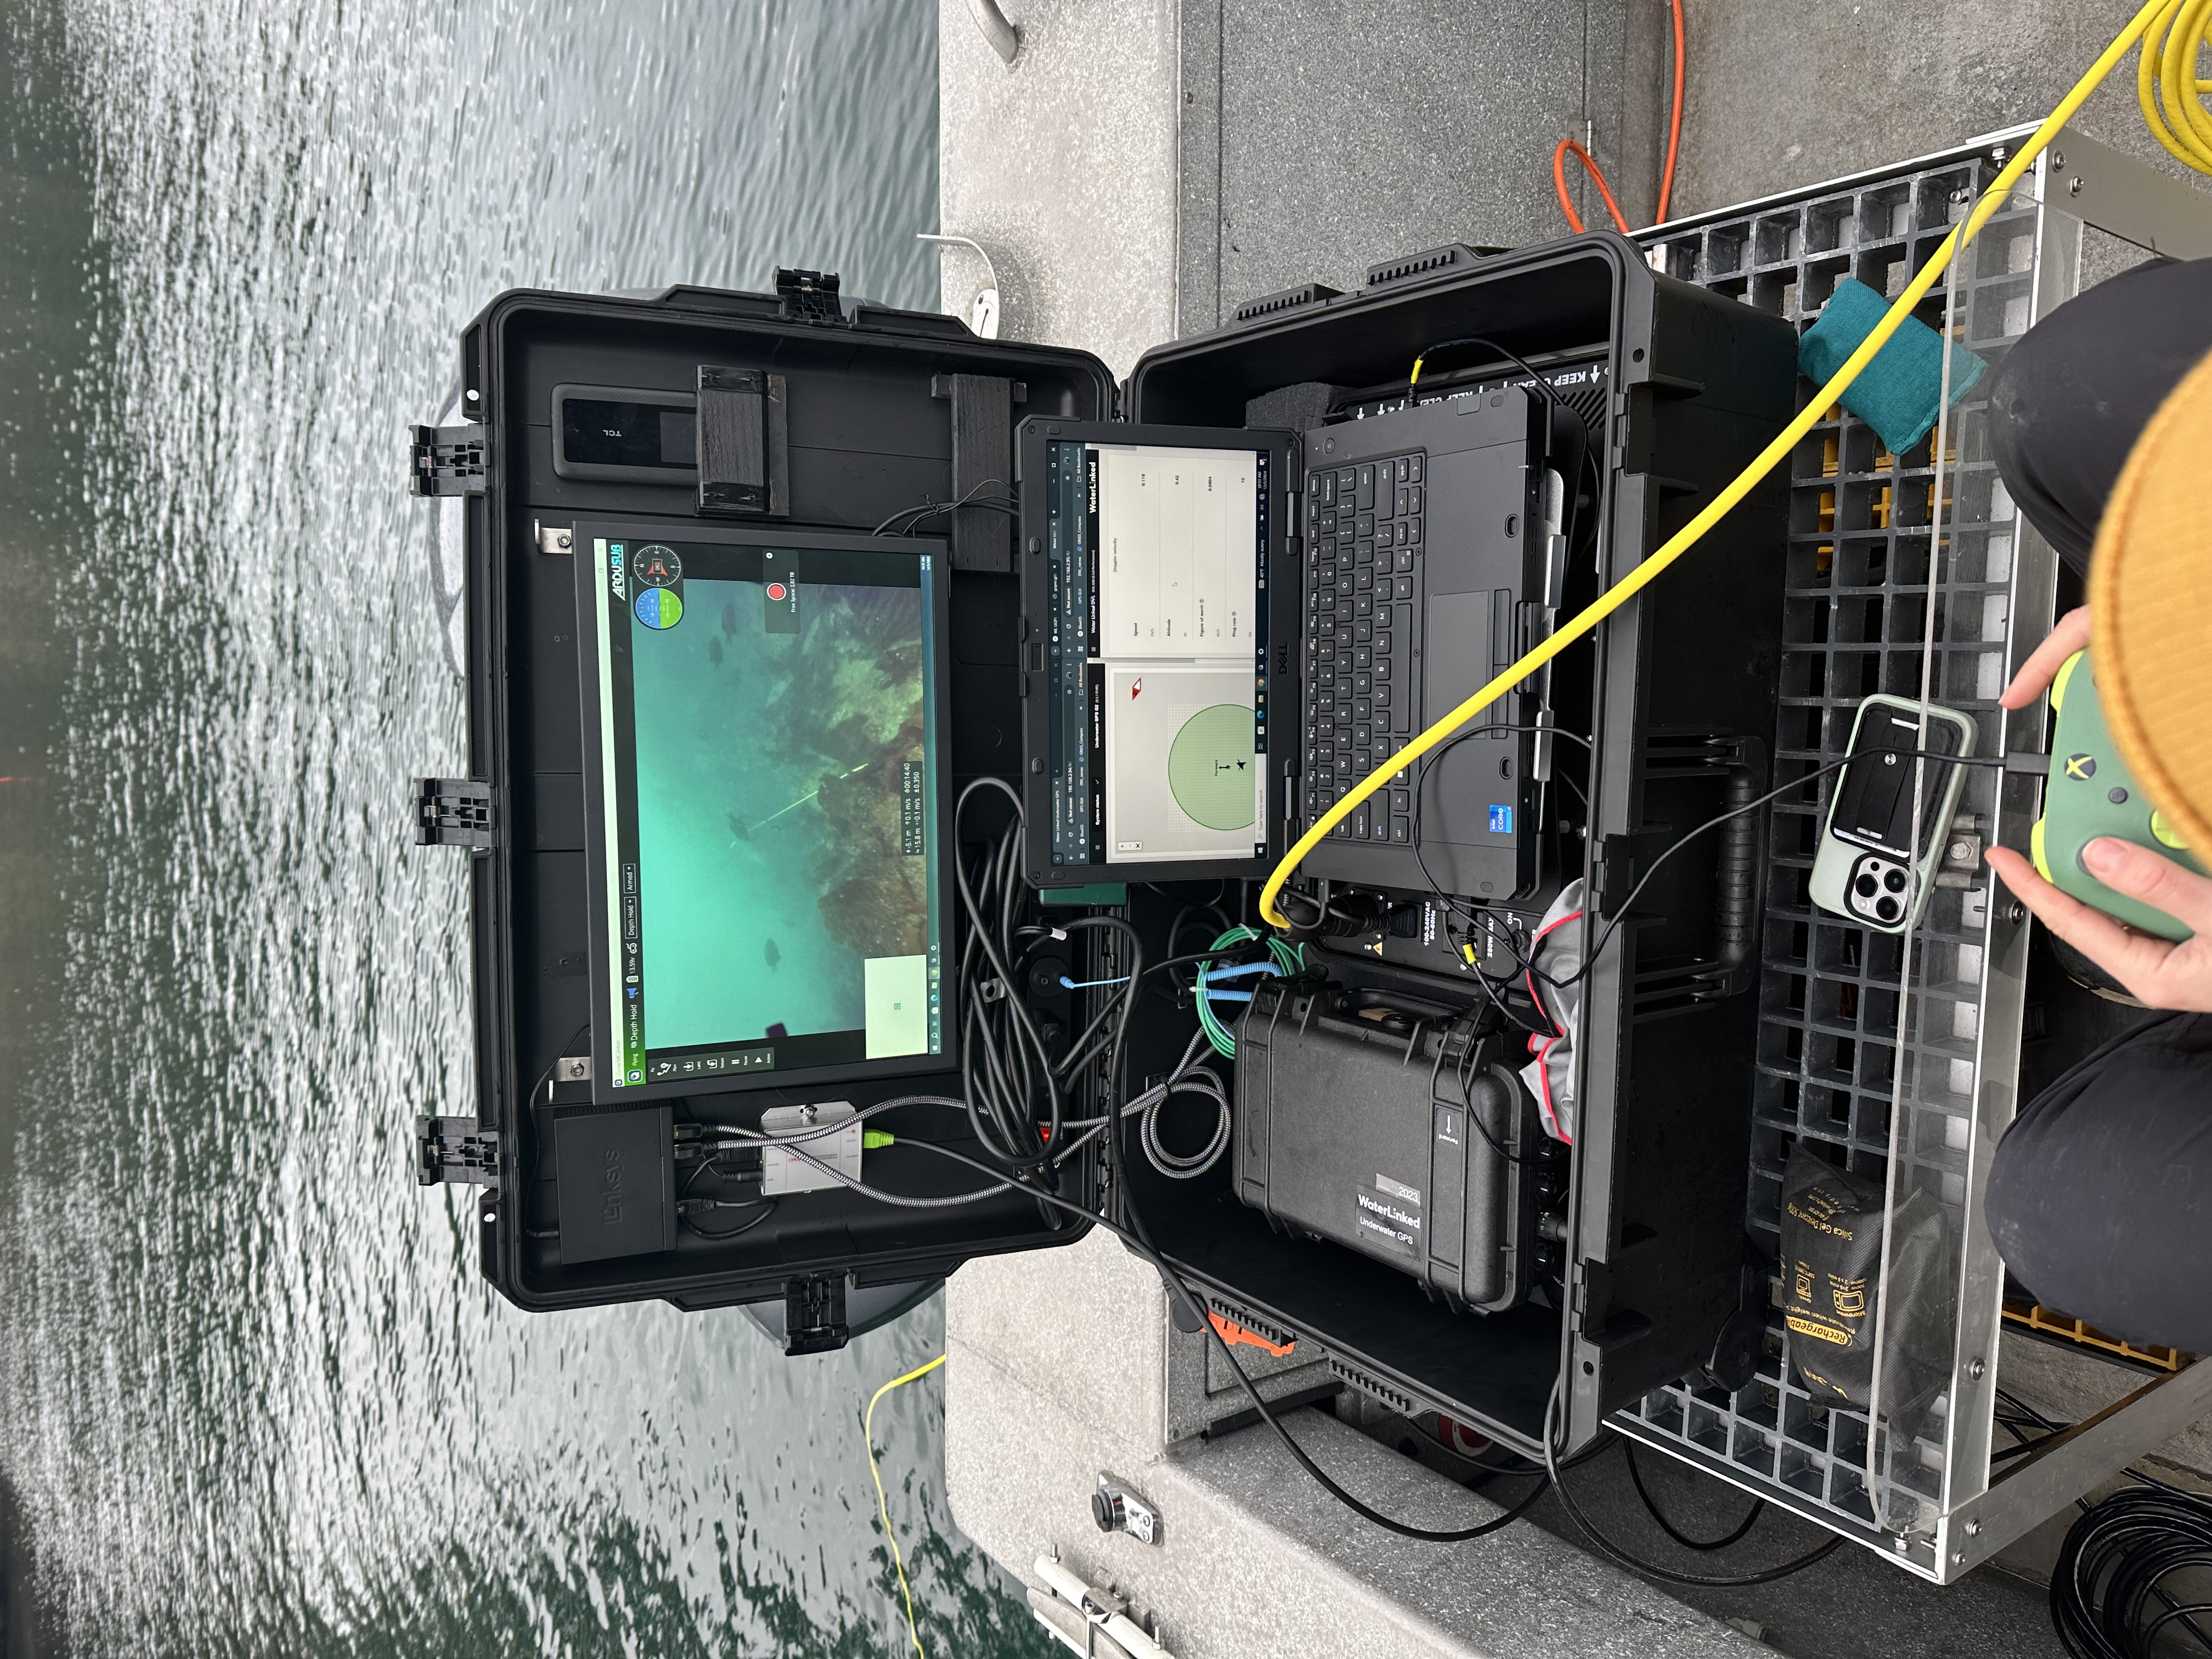
\includegraphics[angle=-90,origin=c,width=\linewidth]{field_methods_2.jpg}
\end{subfigure}
\caption{
The Seattle Aquarium's 24' Aluminum Almar vessel off which we conducted paired 
ROV-diver field surveys.
The vessel's open back deck has been optimized for dive operations such that we 
were able to conduct concurrent diver and ROV surveys. 	
Subfigure (b) depicts the ROV's command console that the topside personnel used 
to conduct ROV surveys. 
}
\label{fig:field_methods}
\end{figure}
\vfil
}

\clearpage

\vbox to \textheight{
\vfil
\begin{figure}[H]
\centering

% max width=\textwidth shrinks the drawing to fit if it would otherwise
% overrun the text block (it does, by ~20mm at this scale), and leaves it
% untouched otherwise
\adjustbox{max width=\textwidth}{%
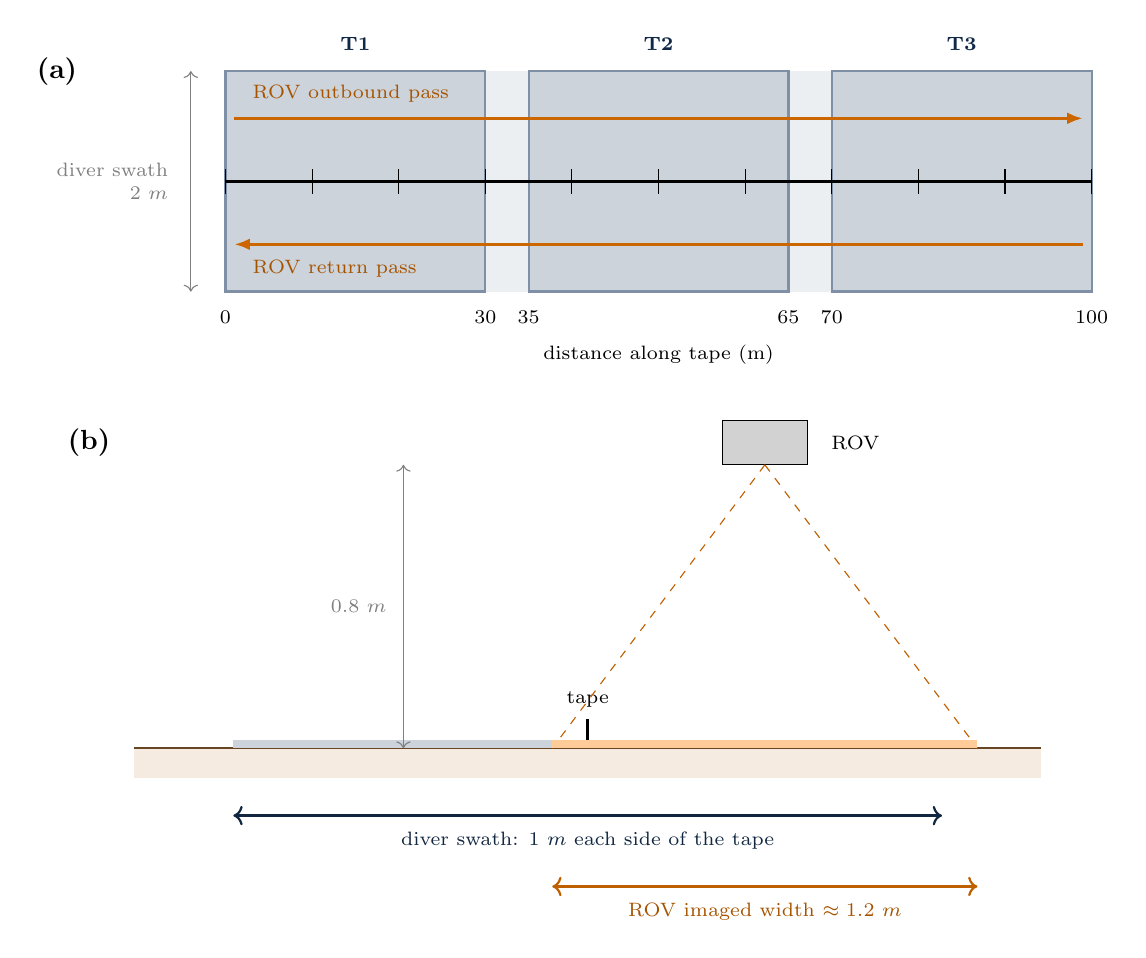
\begin{tikzpicture}[x=1.1mm, y=1mm, font=\small]

%% ------------------------------------------------------------------
%% (a) PLAN VIEW -- the 100 m tape, the three 30 m Reef Check transects,
%%     the diver's 2 m swath, and the ROV's two passes.
%%     Vertical budget: swath spans -14..14; ROV passes sit at +-8 with
%%     their labels at +-9 (inside the swath but clear of both the arrows
%%     and the swath edge); transect tags sit above the box at 18.
%% ------------------------------------------------------------------
\begin{scope}

% diver swath: 1 m either side of the tape
\fill[reportblue!8] (0,-14) rectangle (100,14);

% the three 30 m Reef Check transects (0-30, 35-65, 70-100)
\foreach \s in {0,35,70}{
  \fill[reportblue!22] (\s,-14) rectangle (\s+30,14);
  \draw[reportblue!55, thick] (\s,-14) rectangle (\s+30,14);
}

% ROV passes: one down each side of the tape
\draw[orange!80!black, very thick, -{Latex[length=2mm]}] (1,8) -- (99,8);
\draw[orange!80!black, very thick, -{Latex[length=2mm]}] (99,-8) -- (1,-8);
\node[orange!65!black, anchor=south west, font=\scriptsize] at (2,8.8)
  {ROV outbound pass};
\node[orange!65!black, anchor=north west, font=\scriptsize] at (2,-8.8)
  {ROV return pass};

% the tape itself
\draw[black, very thick] (0,0) -- (100,0);
\foreach \m in {0,10,...,100}{ \draw[black] (\m,-1.6) -- (\m,1.6); }
\foreach \m/\lab in {0/0, 30/30, 35/35, 65/65, 70/70, 100/100}{
  \node[anchor=north, font=\scriptsize] at (\m,-15.2) {\lab};
}
\node[anchor=north, font=\scriptsize] at (50,-19.5) {distance along tape (m)};

% transect tags, clear above the swath box
\foreach \s/\lab in {0/T1, 35/T2, 70/T3}{
  \node[reportblue!75!black, font=\scriptsize\bfseries] at (\s+15,17.5) {\lab};
}

% swath extent annotation, to the left of the tape
\draw[<->, gray] (-4,-14) -- (-4,14);
\node[anchor=east, font=\scriptsize, align=right, gray] at (-5.5,0)
  {diver swath\\$2~m$};

\node[anchor=east, font=\bfseries] at (-16,14) {(a)};

\end{scope}

%% ------------------------------------------------------------------
%% (b) CROSS-SECTION -- diver swath width vs. ROV imaged width.
%%     Scale: 5 units = 1 m, so the 2 m swath spans -5..5, the ROV's
%%     0.8 m altitude is 4 units, and its ~1.2 m footprint is 6 units.
%%     The ROV is drawn centred over the middle of the right-hand side
%%     of the swath, which is where its footprint overruns both the tape
%%     and the outer swath edge -- the point of the panel.
%%     All dimension arrows are stacked below the seafloor so nothing
%%     collides with the vehicle or the cone.
%% ------------------------------------------------------------------
% yshift clears panel (a): (a) descends to -20mm, and (b) rises to +42mm
% above its own origin (the ROV at 4.62 units x 9mm), so -72mm leaves ~10mm
% between them. xshift centres (b) beneath (a), whose midpoint sits near 46mm.
\begin{scope}[xshift=46mm, yshift=-72mm, x=9mm, y=9mm]

% seafloor
\fill[brown!16] (-6.4,-0.42) rectangle (6.4,0);
\draw[brown!55!black, thick] (-6.4,0) -- (6.4,0);

% diver swath footprint on the seafloor
\fill[reportblue!22] (-5,0) rectangle (5,0.12);

% the tape, seen end-on
\draw[black, very thick] (0,0) -- (0,0.42);
\node[anchor=south, font=\scriptsize] at (0,0.44) {tape};

% ROV, flown 0.8 m above the seafloor, over the right-hand side
\fill[gray!35, draw=black] (1.9,4) rectangle (3.1,4.62);
\node[anchor=west, font=\scriptsize] at (3.3,4.31) {ROV};

% camera cone down to the imaged footprint (~1.2 m wide)
\draw[orange!75!black, dashed] (2.5,4) -- (-0.5,0);
\draw[orange!75!black, dashed] (2.5,4) -- (5.5,0);
\fill[orange!40] (-0.5,0) rectangle (5.5,0.12);

% altitude marker, placed left of the vehicle and clear of the cone
\draw[<->, gray] (-2.6,0) -- (-2.6,4);
\node[anchor=east, font=\scriptsize, gray] at (-2.7,2) {$0.8~m$};

% stacked dimension arrows below the seafloor
\draw[<->, reportblue!70!black, thick] (-5,-0.95) -- (5,-0.95);
\node[reportblue!70!black, anchor=north, font=\scriptsize] at (0,-1.05)
  {diver swath: $1~m$ each side of the tape};

\draw[<->, orange!75!black, thick] (-0.5,-1.95) -- (5.5,-1.95);
\node[orange!65!black, anchor=north, font=\scriptsize] at (2.5,-2.05)
  {ROV imaged width $\approx 1.2~m$};

\node[anchor=east, font=\bfseries] at (-6.6,4.31) {(b)};

\end{scope}

\end{tikzpicture}%
}

\caption{
Survey geometry for the paired ROV--diver comparison.
\textbf{(a)} Plan view of one depth zone. A single contiguous $100~m$ tape is
laid along the seafloor, within which the three $30~m$ Reef Check transects
(T1--T3, darker blue) are surveyed at $0$--$30~m$, $35$--$65~m$, and
$70$--$100~m$, leaving $5~m$ between adjacent transects for approximate
statistical independence. Divers survey a $1~m$ swath on each side of the tape
($2~m$ total). The ROV flies the full $100~m$ twice --- once down each side of
the tape --- so that both halves of the surveyed area are imaged, and returns
along the same tape rather than repositioning, which also reduces entanglement
risk in \textit{Nereocystis}. This full arrangement is repeated at both the
shallow ($5~m$) and deep ($10~m$) zones at each site, giving six transects per
site per season.
\textbf{(b)} Cross-section through the tape, showing why the two platforms do
not sample exactly the same width. Flown at a fixed $0.8~m$ altitude, the
ROV's cropped GoPro footprint is approximately $1.2~m$ wide, against the
diver's $1~m$ per side --- roughly $0.2~m$ of additional width per pass. On
flat seafloor this is a simple linear increase in area surveyed; along complex,
sloping terrain such as the Elliott Bay Marina breakwater it can be
substantially non-linear, and it is one of the mechanisms we invoke in the
\textit{Discussion} to explain the ROV's consistent tendency toward higher
invertebrate counts. Neither panel is drawn to scale.
}
\label{fig:survey_geometry}
\end{figure}
\vfil
}

\clearpage


\vbox to \textheight{%
\vfil
\begin{figure}[H]
\centering
\begin{subfigure}[t]{0.48\textwidth}
\centering
\textbf{(a)}\par
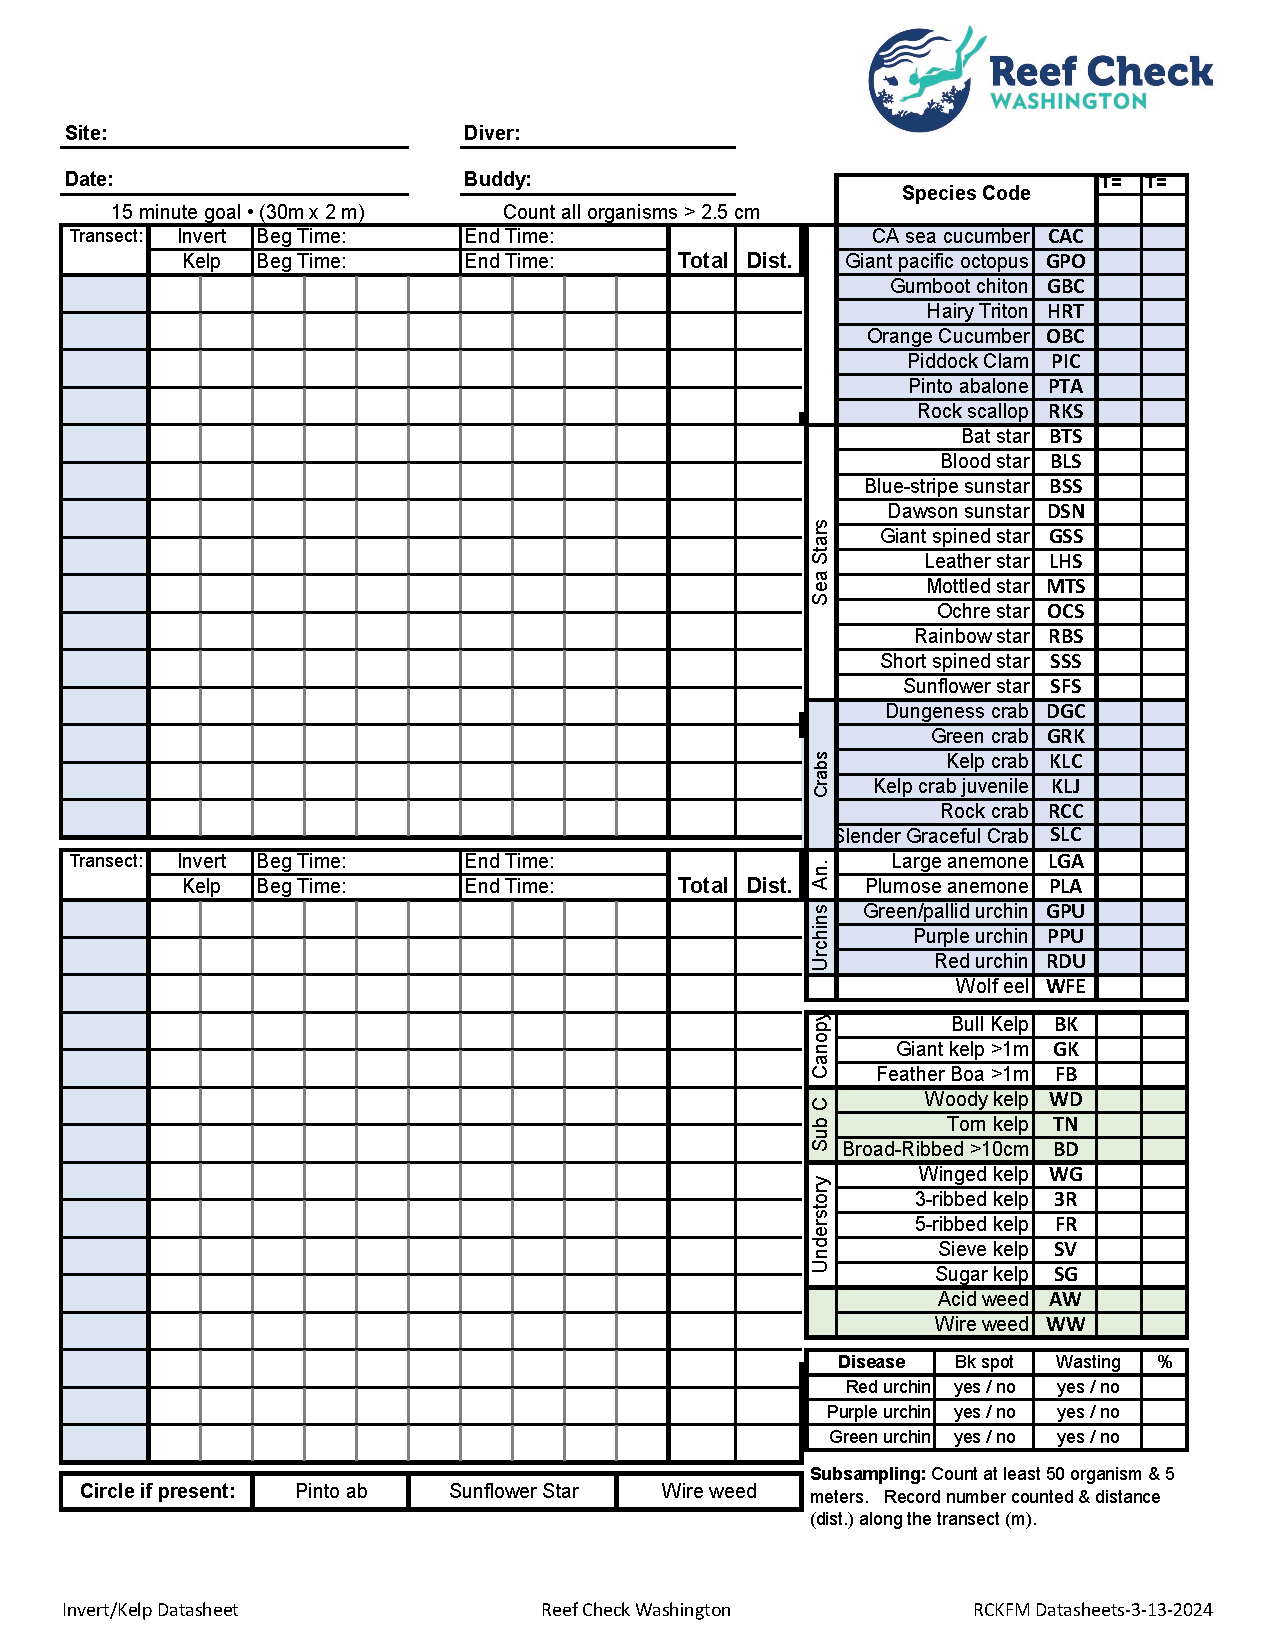
\includegraphics[width=\linewidth]{InvertKelp.pdf}
\end{subfigure}
\hspace{0.01\textwidth}
\begin{subfigure}[t]{0.48\textwidth}
\centering
\textbf{(b)}\par
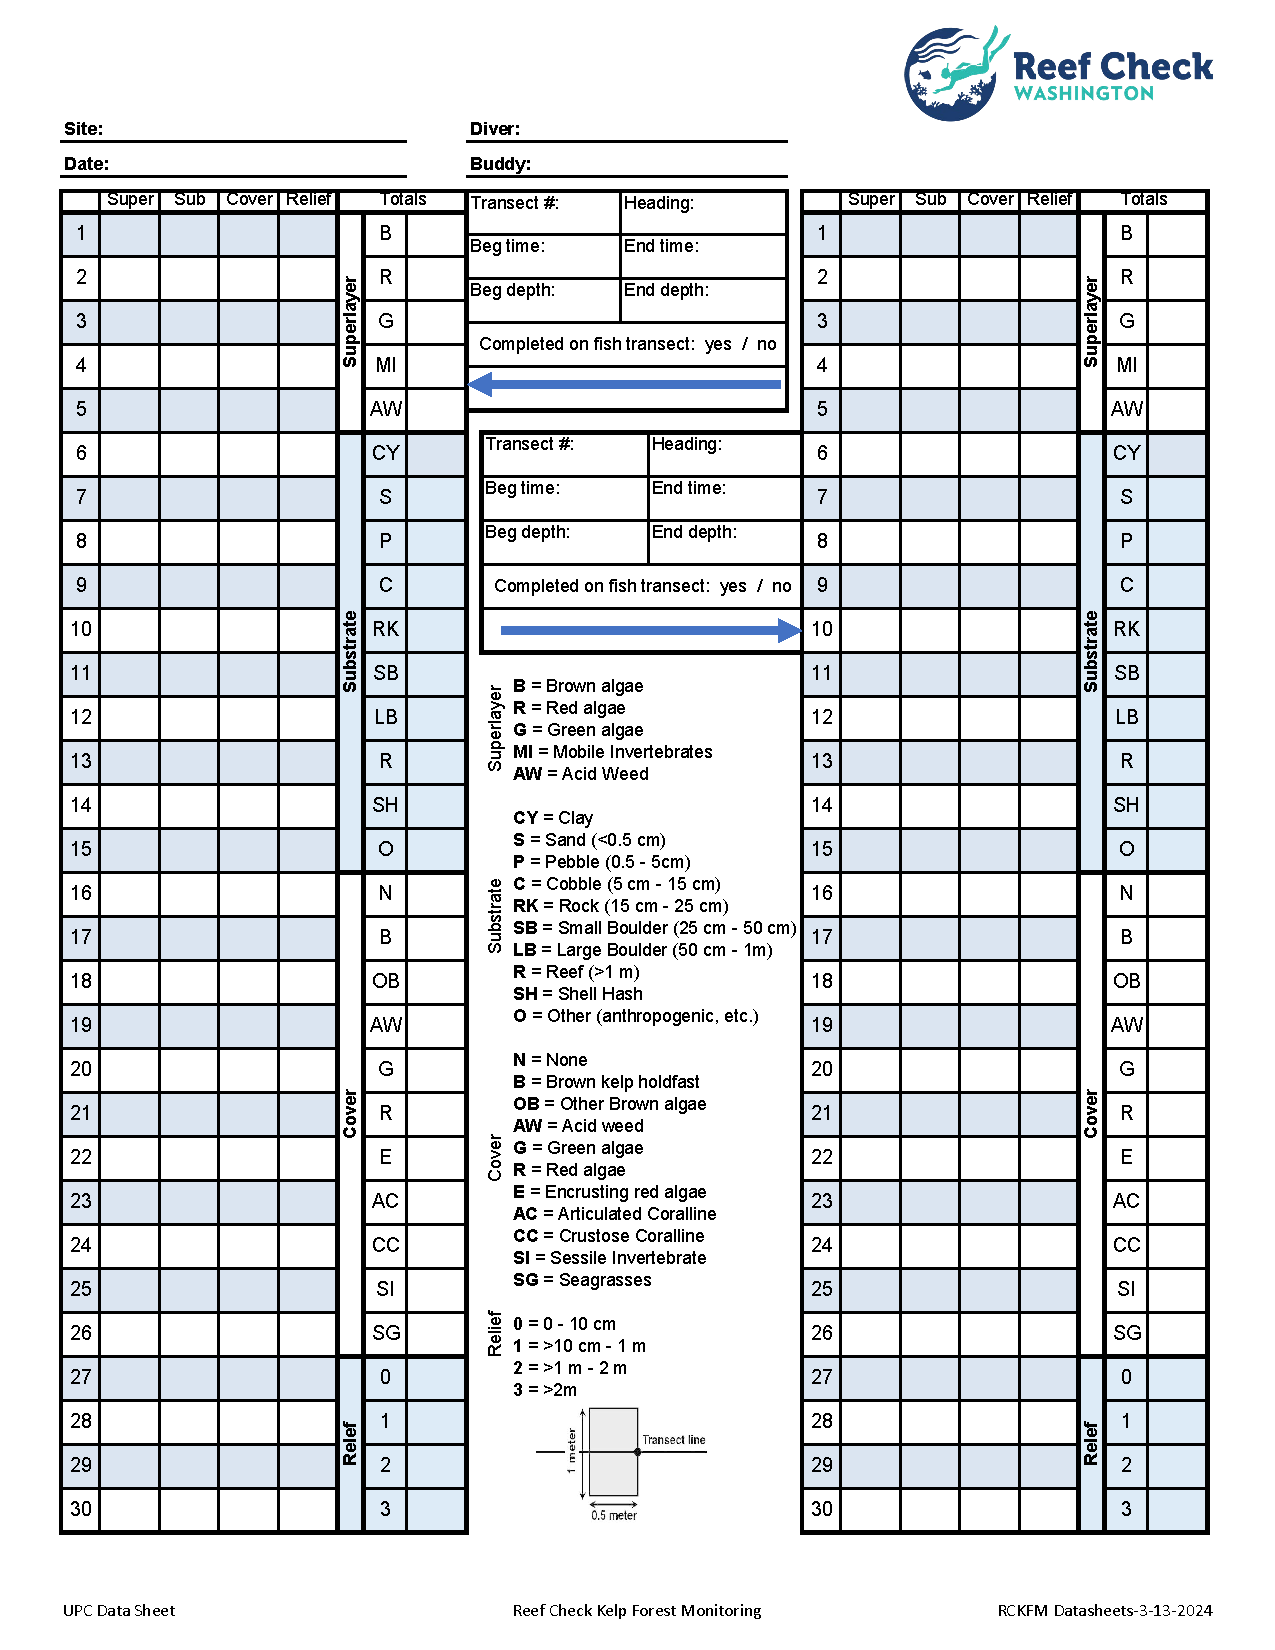
\includegraphics[width=\linewidth]{UPC.pdf}
\end{subfigure}
\caption{
Reef Check Washington's (a) 2024 kelp/invert swath and (b) UPC data sheets used 
as part of this methods comparison.
}
\label{fig:data_sheets}
\end{figure}
\vfil
}

\clearpage

\vbox to \textheight{%
\vfil
\begin{figure}[H]
\centering
\begin{tikzpicture}
\clip (0,0) rectangle (0.63\textwidth,0.42\textwidth);
\node[anchor=center,inner sep=0] at (0.315\textwidth,0.21\textwidth)
{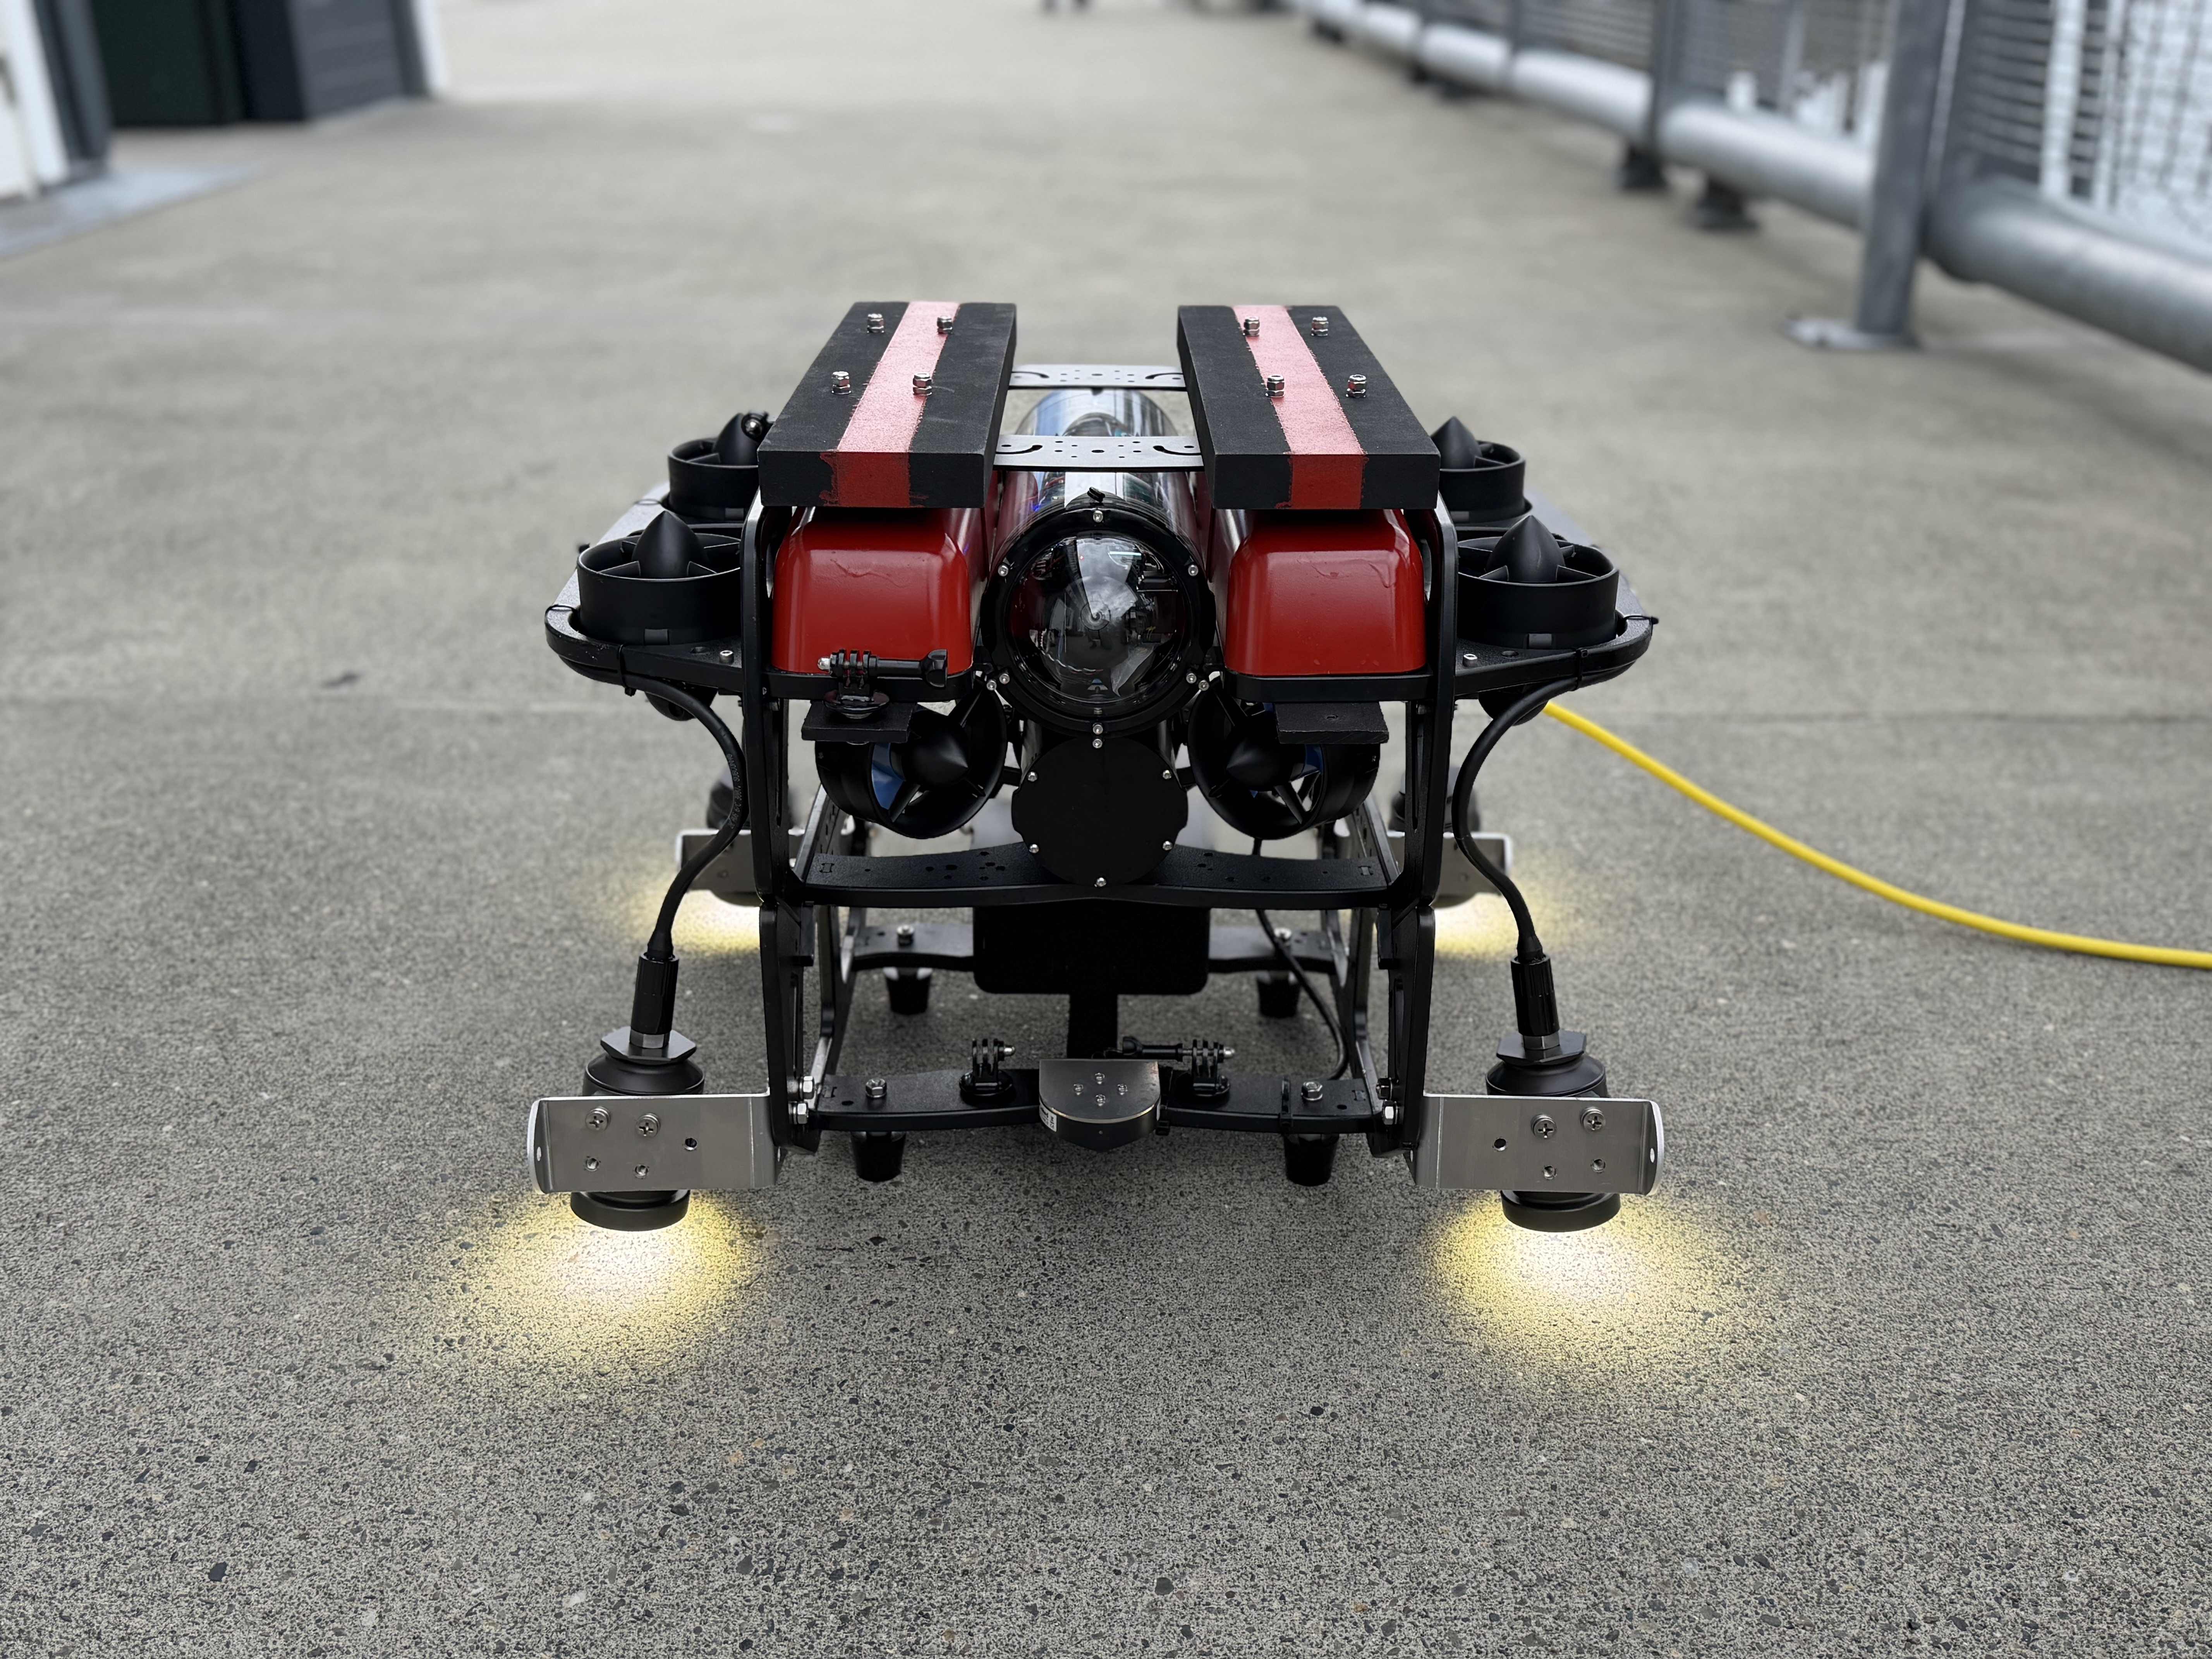
\includegraphics[width=0.63\textwidth]{Lutris_1.jpeg}};
\end{tikzpicture}
\vspace{0.005\textheight}
\begin{tikzpicture}
\clip (0,0) rectangle (0.63\textwidth,0.42\textwidth);
\node[anchor=center,inner sep=0] at (0.315\textwidth,0.21\textwidth)
{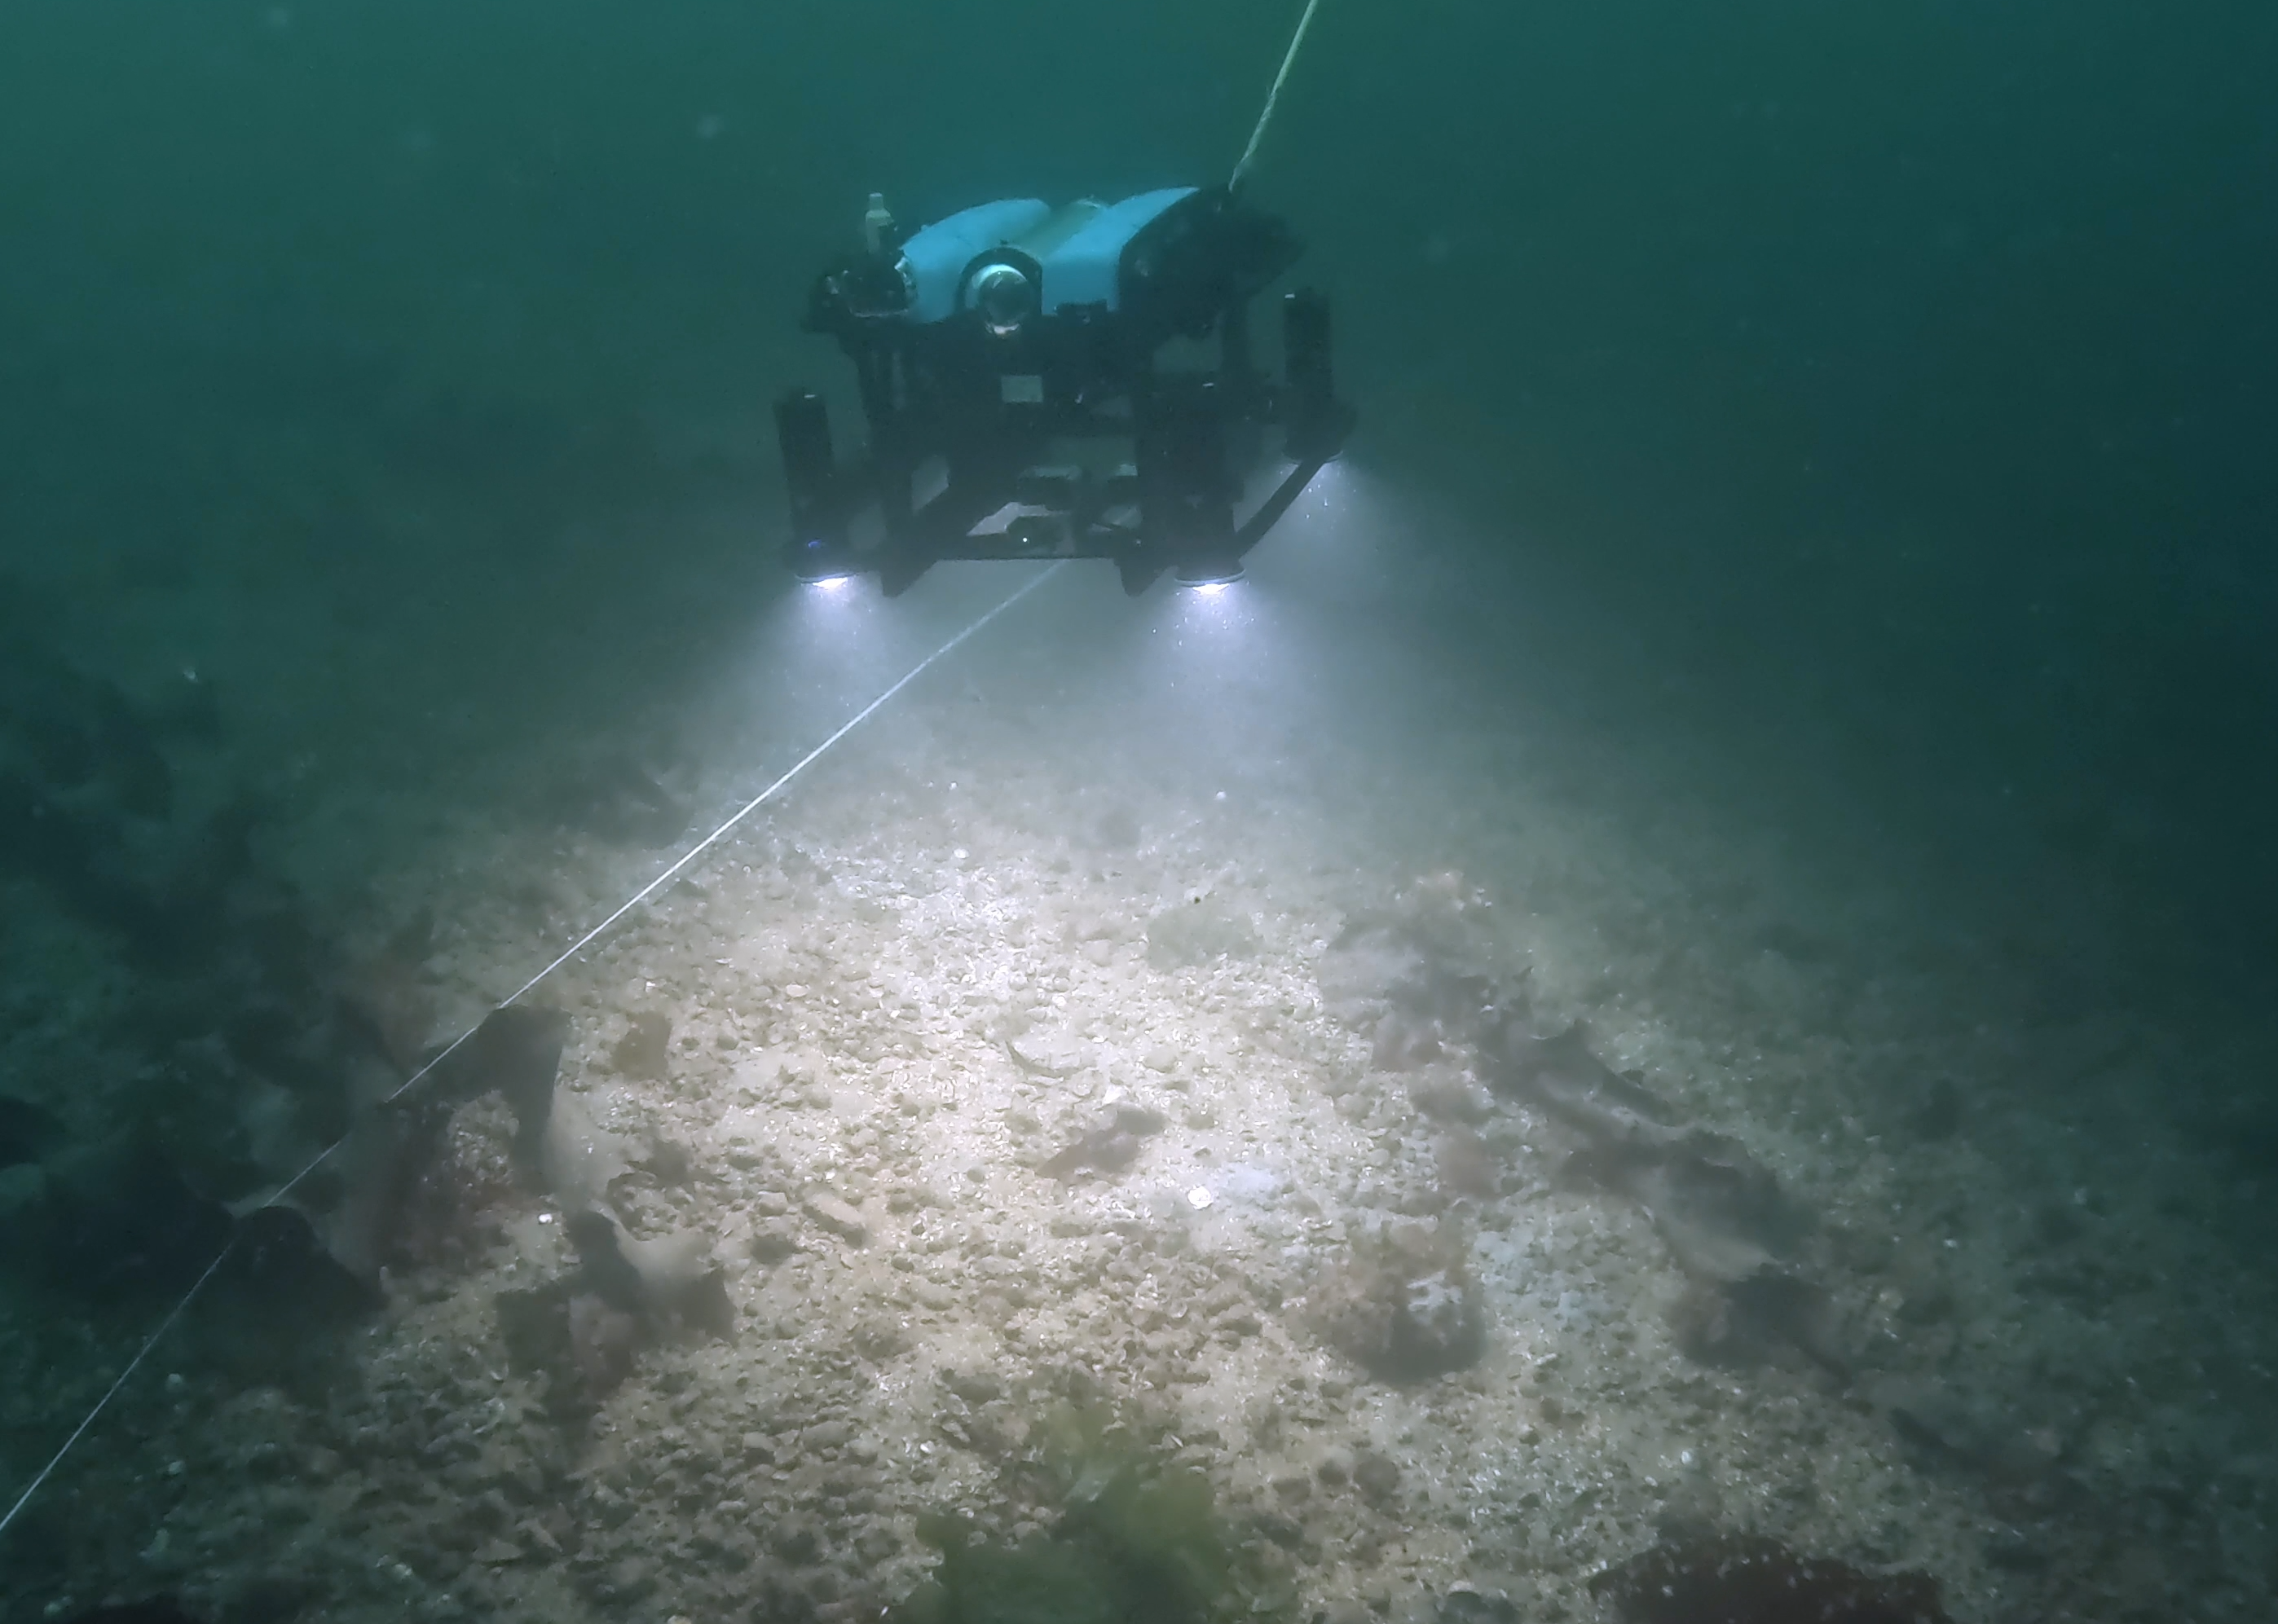
\includegraphics[width=0.63\textwidth]{Lutris_2.PNG}};
\end{tikzpicture}
\vspace{0.005\textheight}
\begin{tikzpicture}
\clip (0,0) rectangle (0.63\textwidth,0.42\textwidth);
\node[anchor=center,inner sep=0] at (0.315\textwidth,0.21\textwidth)
{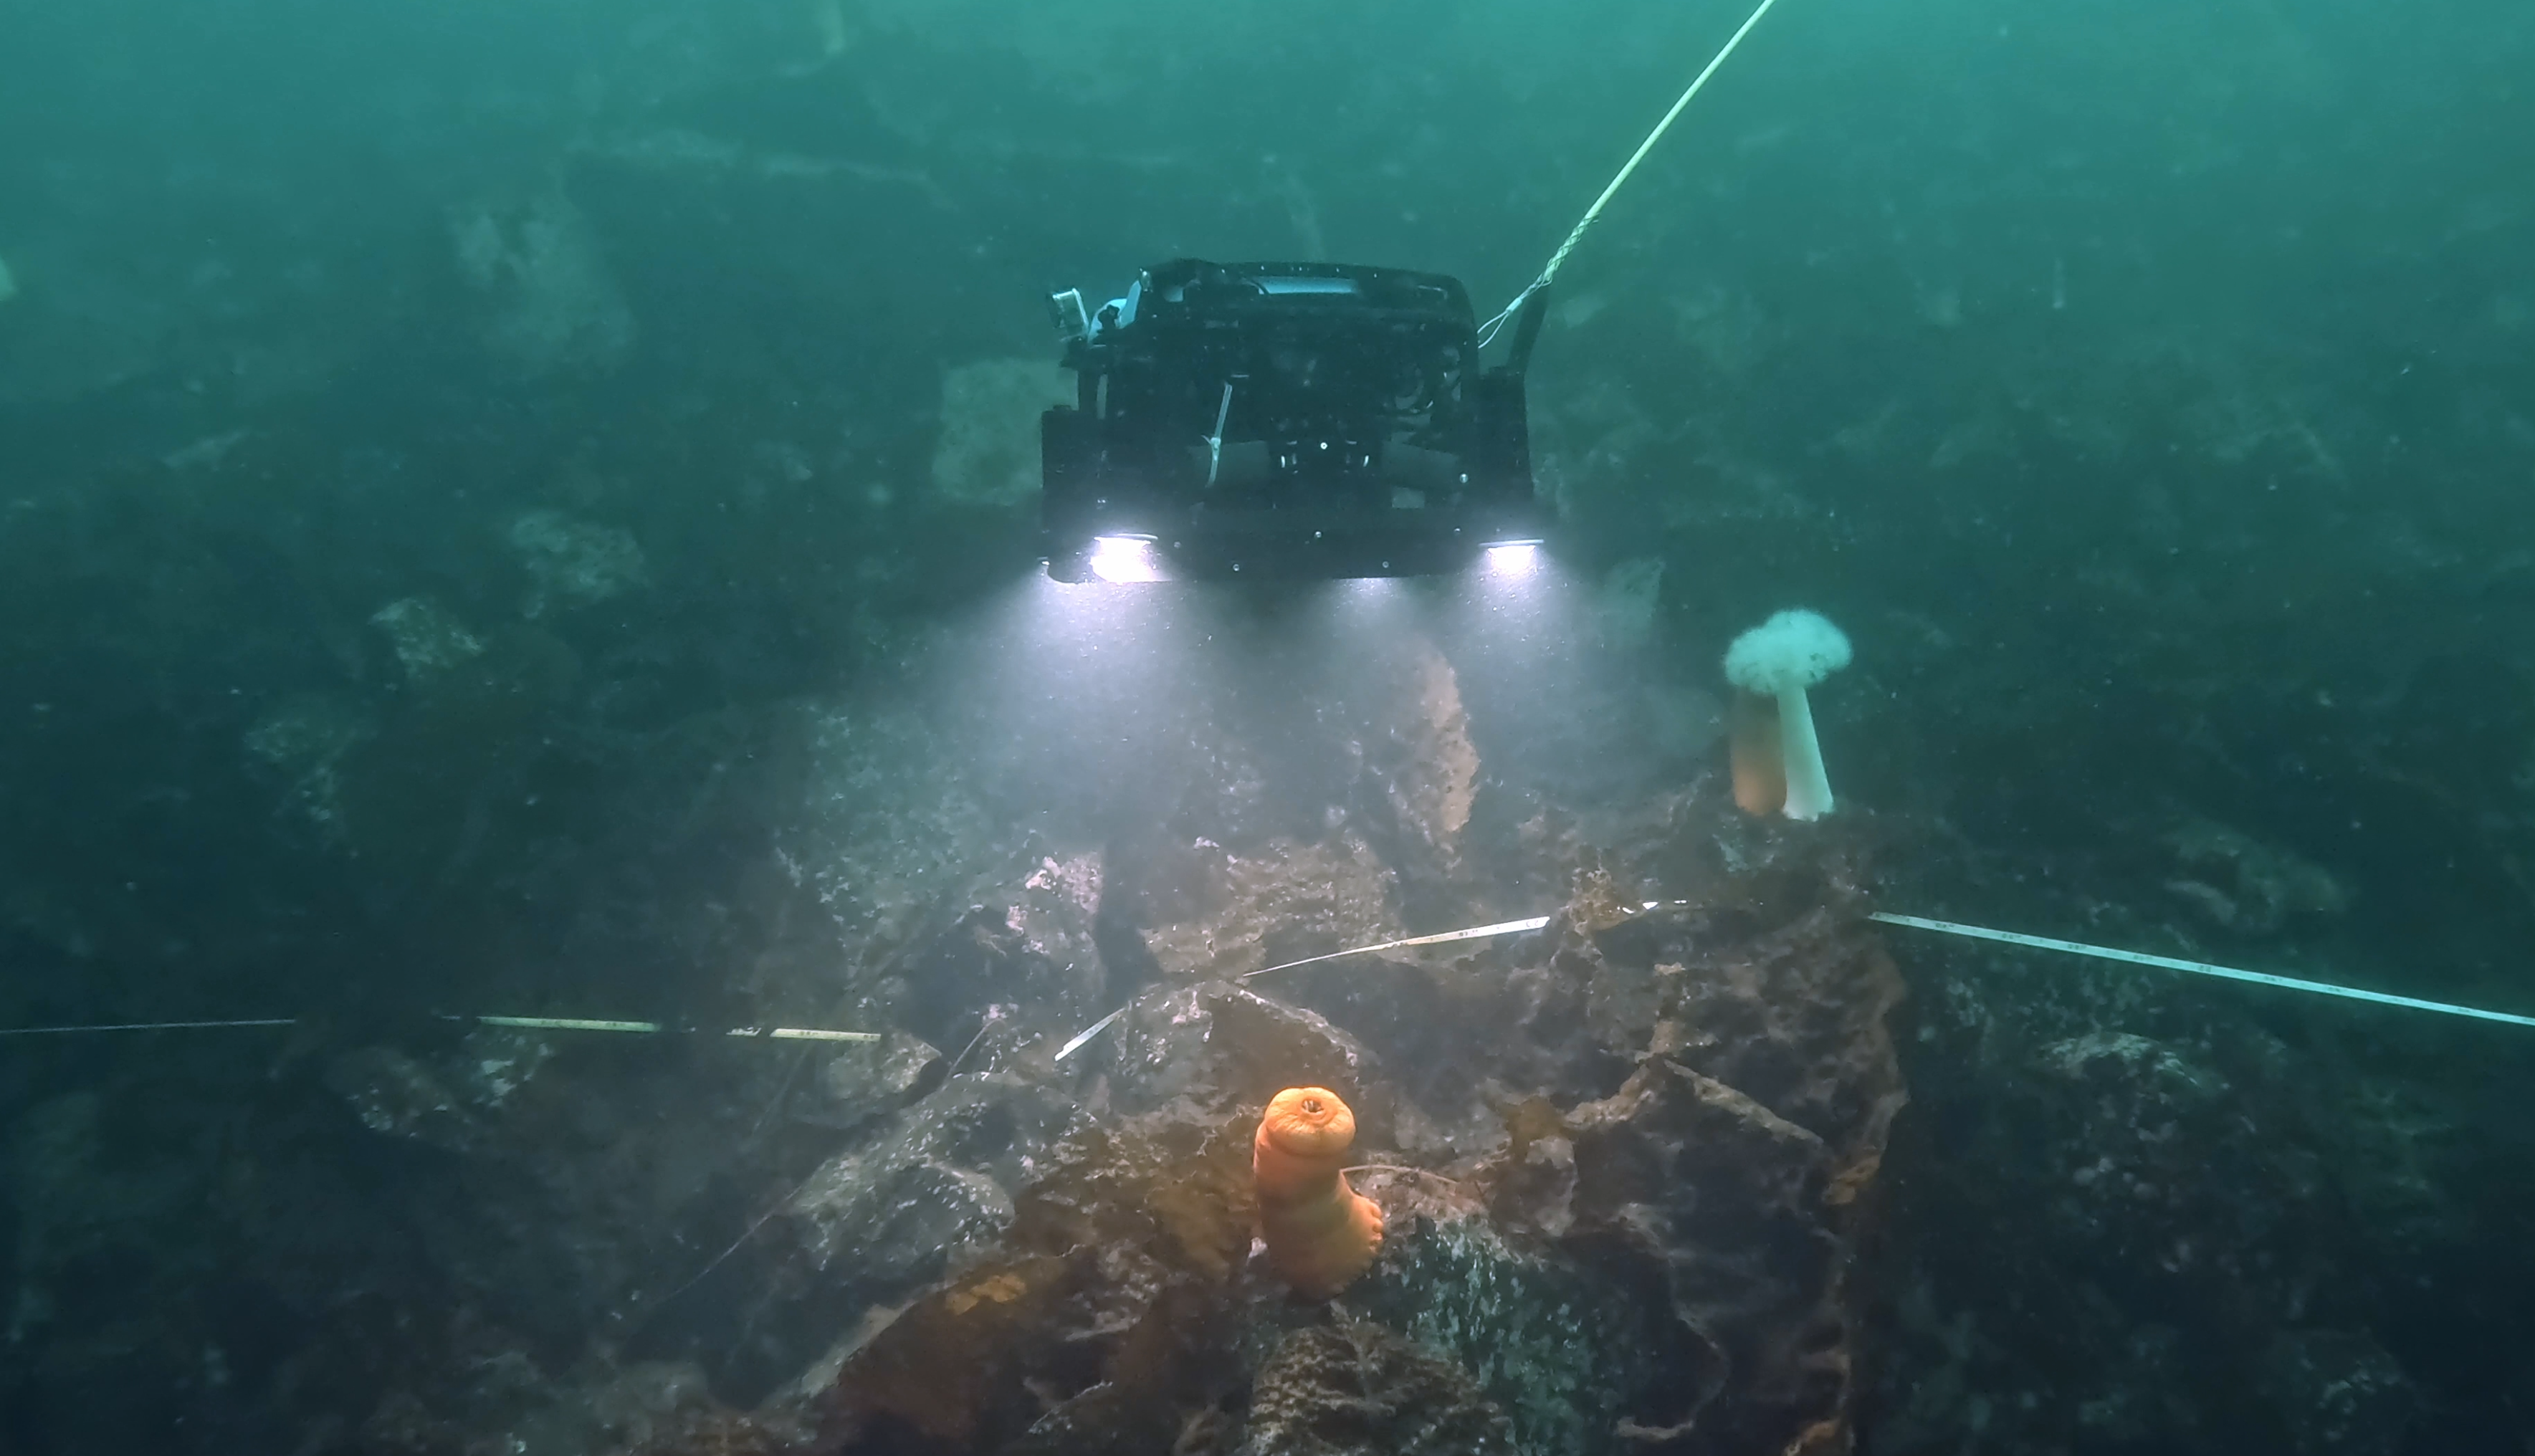
\includegraphics[height=0.42\textwidth]{Lutris_3.PNG}};
\end{tikzpicture}
\caption{
Top: ROV \textit{Lutris} in its $V4$ configuration with integrated lighting 
(see \cite{Randell:2026aa} for details about the various hardware 
configurations comprising the $V1$---$V4$ ROV iterations).
ROV \textit{Lutris} in an earlier $V3$ configuration (integrated power and 
battery-powered diver lights) at Centennial Park (middle) and Elliott Bay 
Marina breakwater (bottom). 
}
\label{fig:ROV}
\end{figure}
\vfil
}

\clearpage

\vbox to \textheight{
\vfil
\begin{figure}[H]
\centering
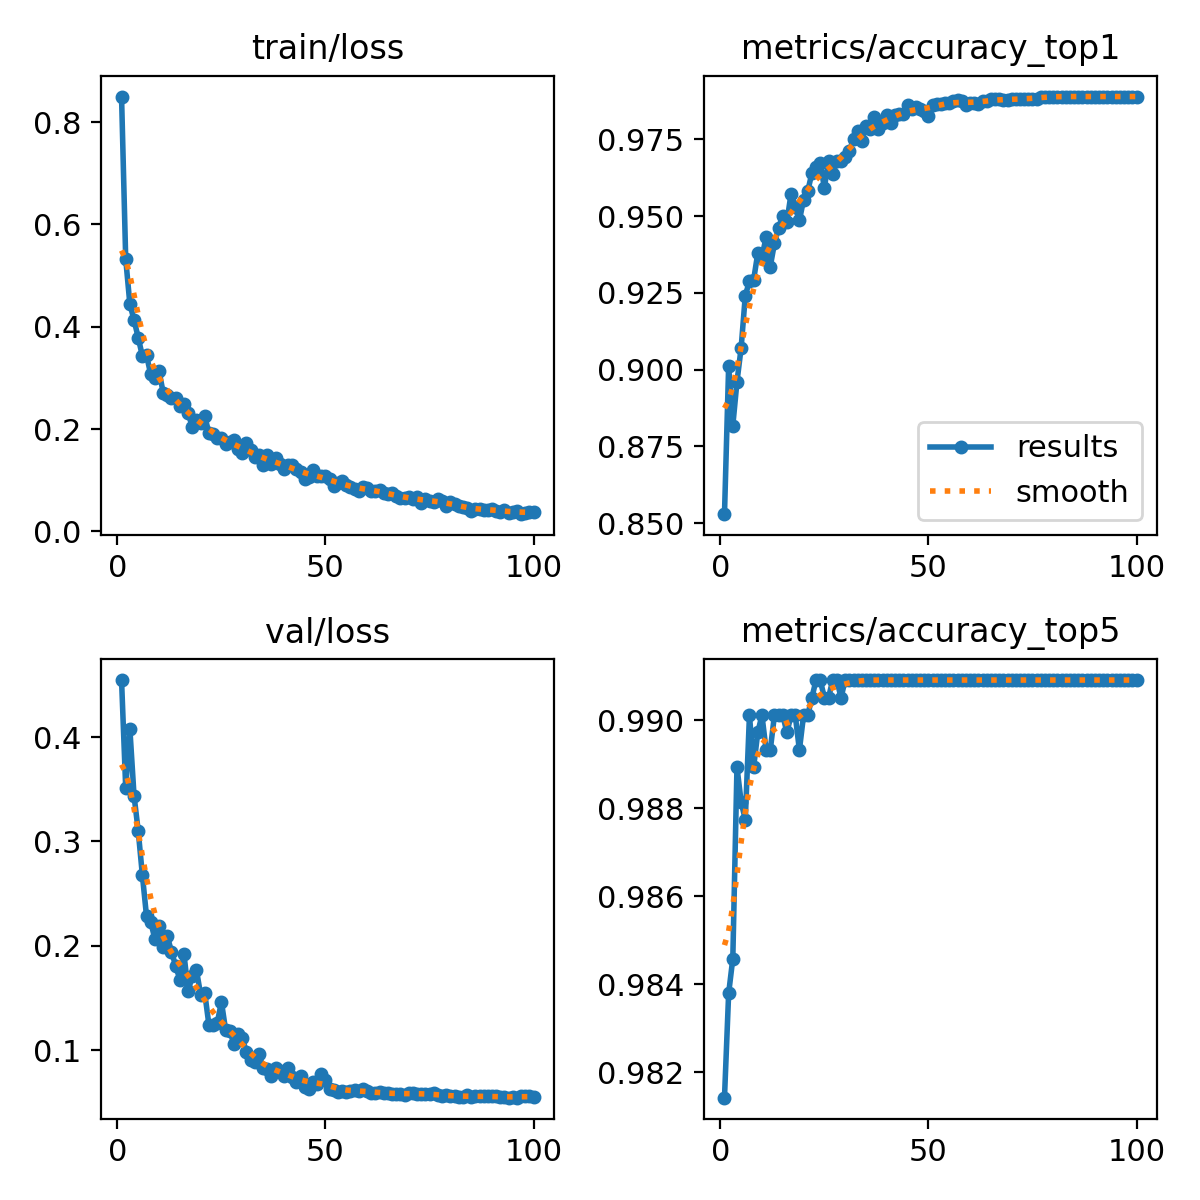
\includegraphics[width=0.85\textwidth]{results.png}
\caption{
Training and validation metrics across 100 training epochs for the 
Elliott Bay CoralNet-Toolbox percent-cover classification model 
(YOLO11s-cls).
Top row: training loss (left) and validation loss (right).
Bottom row: top-1 (left) and top-5 (right) validation accuracy.
Dotted lines show a smoothed trend; solid lines show raw per-epoch 
values.
Final epoch (100): training loss 0.025, validation loss 0.136, top-1 
accuracy 96.58\%, top-5 accuracy 99.82\%.
}
\label{fig:toolbox_training}
\end{figure}
\vfil
}

\clearpage

\vbox to \textheight{
\vfil
\begin{figure}[H]
\centering
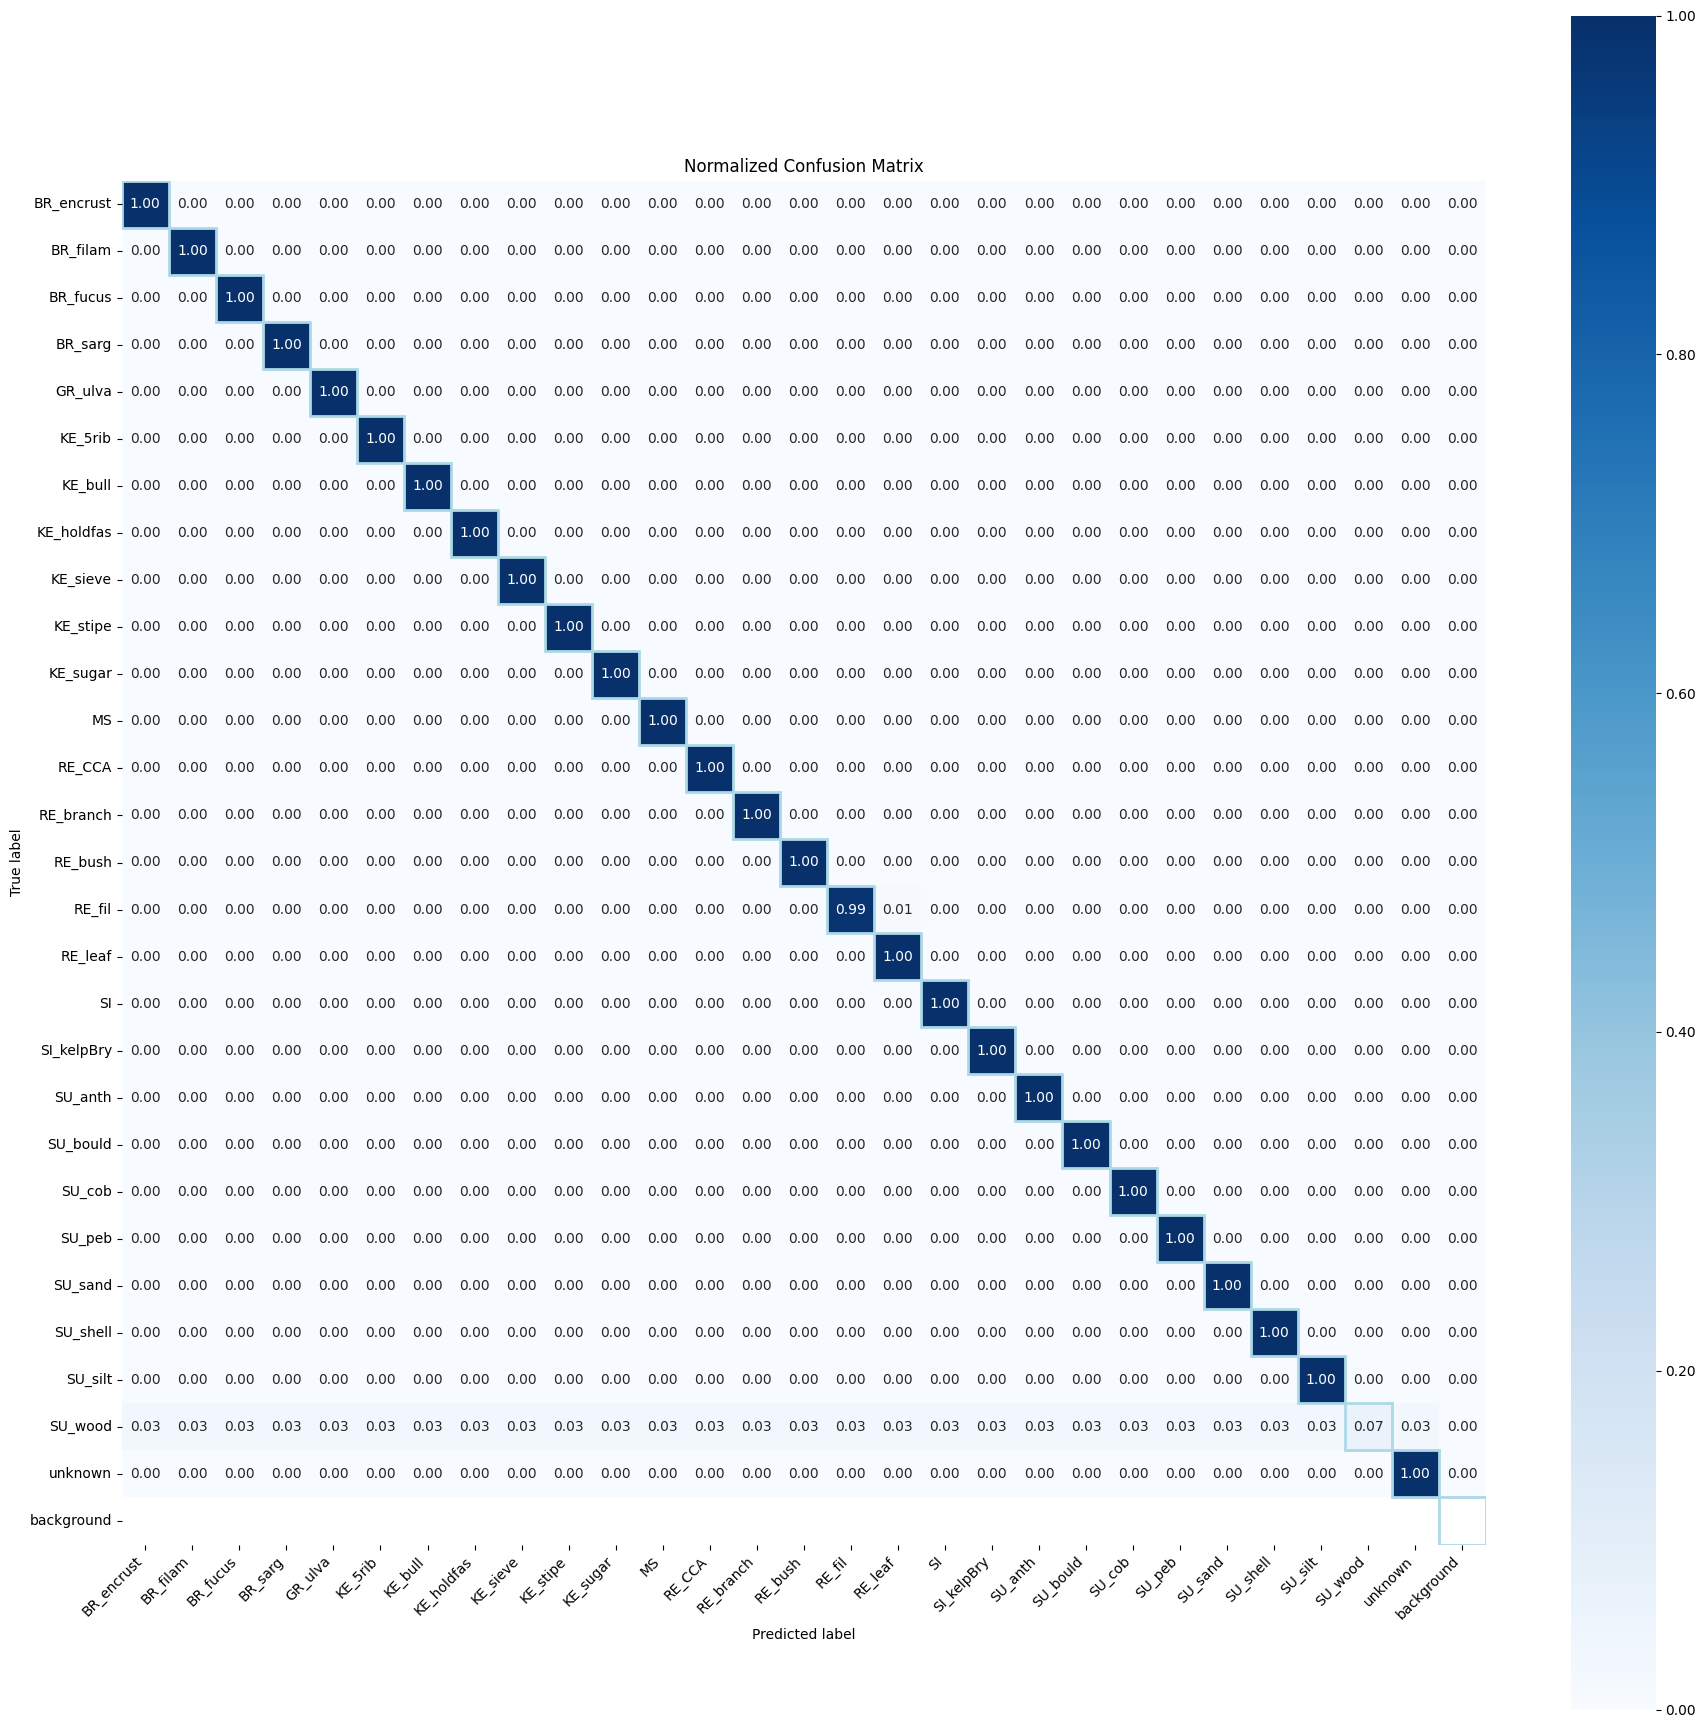
\includegraphics[width=0.85\textwidth]{confusion_matrix_normalized.png}
\caption{
Normalized confusion matrix for the Elliott Bay CoralNet-Toolbox
percent-cover classification model, evaluated on its held-out test set.
Rows show true labels; columns show predicted labels.
Diagonal values indicate the proportion of correctly classified patches
for each category (recall); off-diagonal values indicate
misclassification rates.
This evaluation reflects an earlier iteration of the model, trained on a
category scheme that has since been revised to the 27 categories in
\tabref{tab:toolbox_categories}; current test-set performance by category is
reported there.
}
\label{fig:toolbox_confusion}
\end{figure}
\vfil
}

\clearpage

\vbox to \textheight{
\vfil
\begin{figure}[H]
\centering
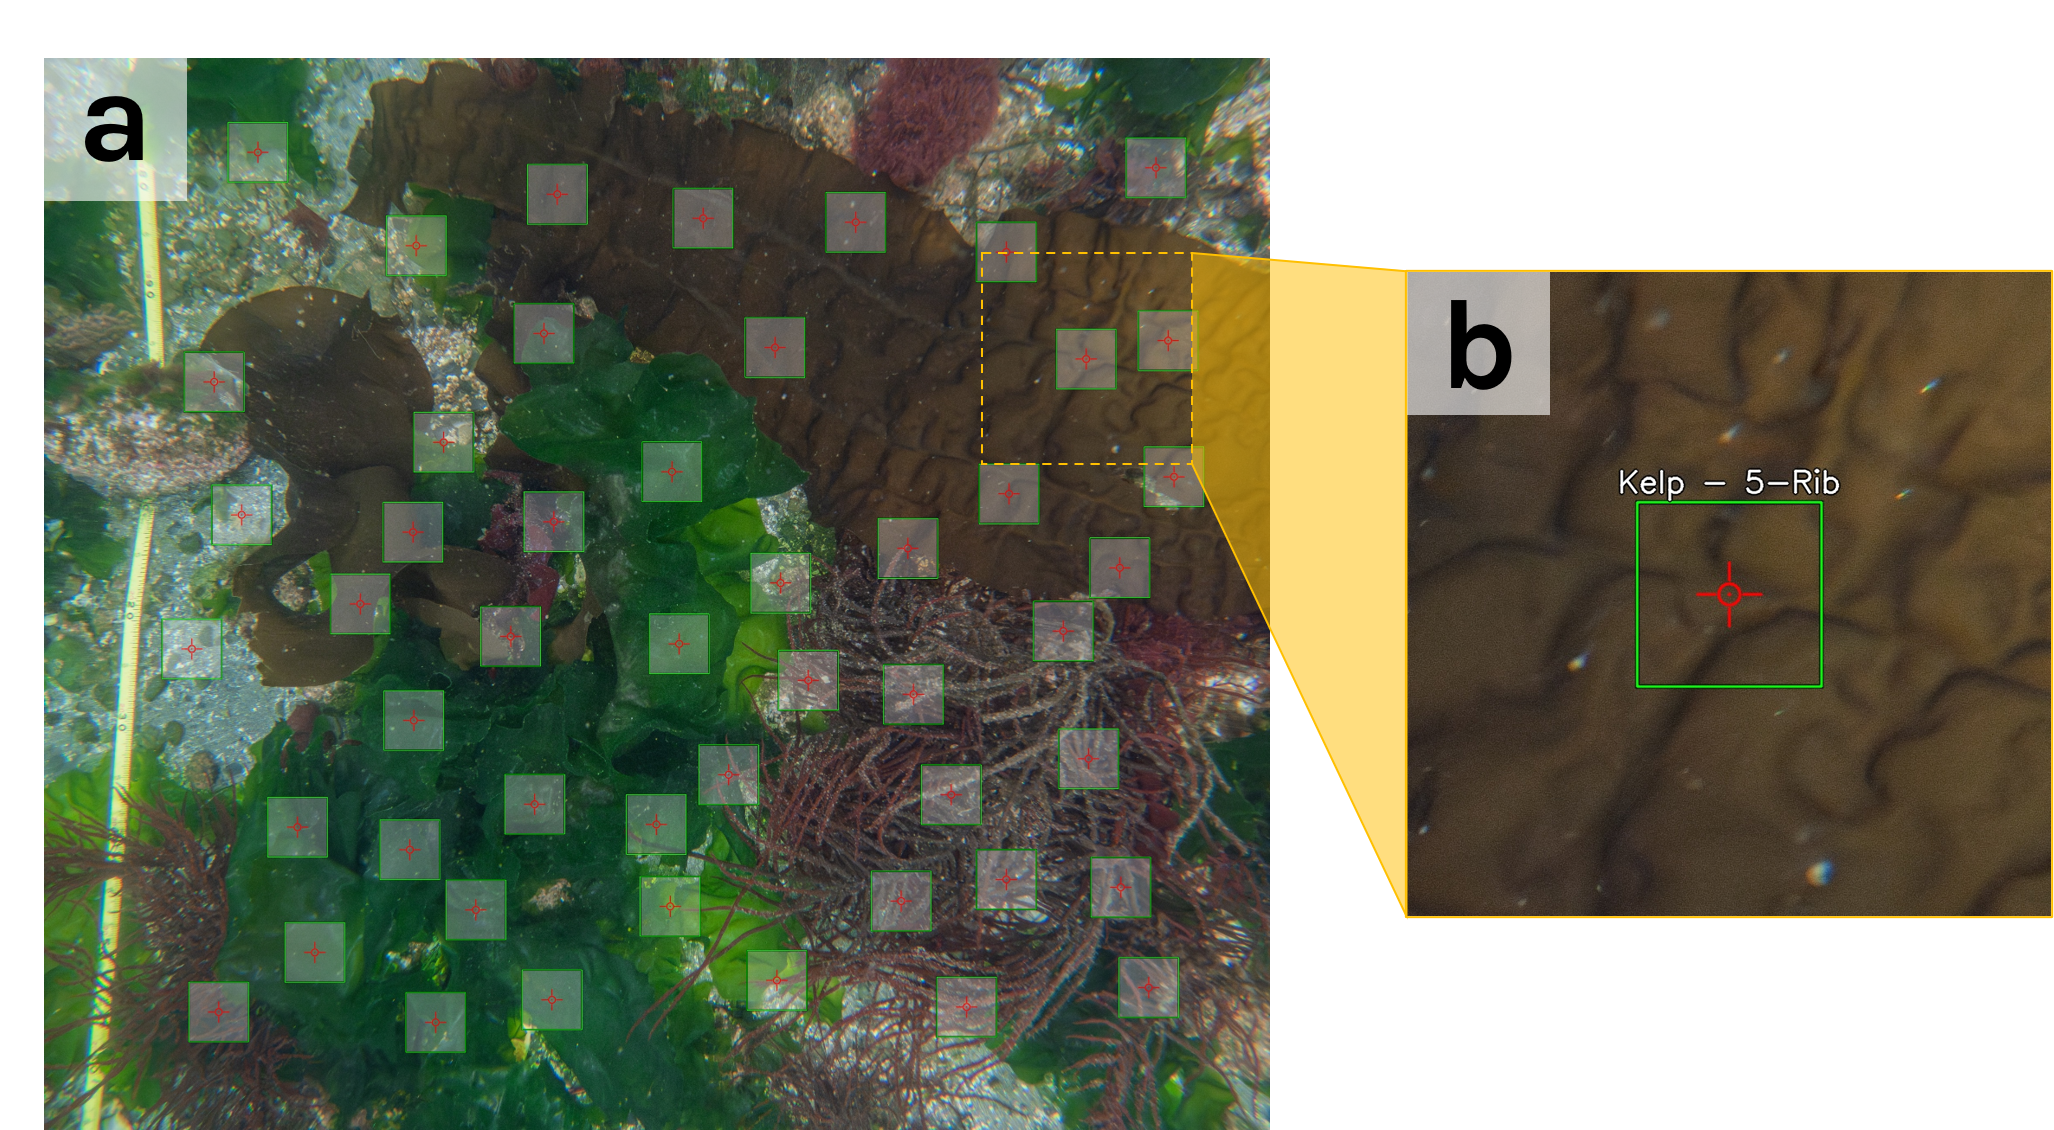
\includegraphics[width=0.95\textwidth]{image_sampling.png}
\caption{
(a) A single ROV photograph with 50 randomly distributed percent-cover patches, 
each of which is comprised of 224 x 224 pixels.
(b) A single ``subject" --- the individual percent-cover data point we provide 
to Kelp Quest volunteers to review. 
Each subject is comprised of a red target that provides the point-sampling 
visual guide, a green box delineating the 224 x 224 patch of pixels viewed by 
the ML algorithm, and a surrounding image area that we use to provide context 
to help visually identify the subject.  
Note that this figure was created in PowerPoint to serve as a visual example,
and therefore the image patches were ``haphazardly" placed, not truly randomly
generated, as they are for our real ROV survey imagery.
}
\label{fig:image_sampling}
\end{figure}
\vfil
}

\clearpage

\vbox to \textheight{
\vfil
\begin{table}[H]
\centering
\caption{
Percent-cover categories trained in our CoralNet-Toolbox classification
model \citep{Pierce:2025aa}, grouped by broad category type. 
Training and validation patch counts reflect a 70\%/20\% split of
the total annotated patches available for each category.
Testing patch counts and test-set accuracy (recall) are the actual 
test-set sizes and results from evaluating the current production model 
(\texttt{EB\_HSIL\_2025\_01\_19}), which was trained on an earlier 
annotation export.
}
\label{tab:toolbox_categories}
\begin{tabular}{llcccc}
\toprule
\textbf{Group} & \textbf{Category} &
\makecell{\textbf{Training}\\\textbf{patches}} &
\makecell{\textbf{Validation}\\\textbf{patches}} &
\makecell{\textbf{Testing}\\\textbf{patches}} & \textbf{\% Accuracy} \\
\midrule
\multirow{7}{*}{Kelp} & Sieve kelp (\textit{Agarum}) & 527 & 
151 & 76 & 
100.0 \\
& Sugar kelp (\textit{Saccharina}) & 869 & 248 & 115 & 100.0 
\\
& Five-ribbed kelp (\textit{Costaria}) & 347 & 99 & 51 & 100.0 
\\
& Bull kelp blade & 27 & 8 & 4 & 100.0 \\
& Kelp stipe & 340 & 97 & 50 & 100.0 \\
& Kelp holdfast & 113 & 32 & 17 & 100.0 \\
& Bryozoan-encrusted kelp & 179 & 51 & 27 & 100.0 \\
\midrule
\multirow{4}{*}{\makecell{Brown\\algae}} & Filamentous brown algae &
34 & 10 & 5 & 100.0 \\
& Encrusting brown algae & 27 & 8 & 4 & 100.0 \\
& Rockweed (\textit{Fucus}) & 59 & 17 & 9 & 100.0 \\
& \textit{Sargassum muticum} & 414 & 118 & 61 & 100.0 \\
\midrule
\multirow{5}{*}{\makecell{Red\\algae}} & Branching red algae & 708 &
202 & 103 & 100.0 \\
& Crustose coralline algae & 408 & 117 & 59 & 100.0 \\
& Leafy red algae & 739 & 211 & 106 & 100.0 \\
& Filamentous red algae & 566 & 162 & 83 & 98.8 \\
& Bushy/cylindrical red algae & 465 & 133 & 67 & 100.0 \\
\midrule
\makecell{Green\\algae} & \textit{Ulva} spp. & 279 & 80 &
41 & 100.0 \\
\midrule
\multirow{7}{*}{Substrate} & Pebble & 399 & 114 & 58 & 100.0 \\
& Cobble & 270 & 77 & 40 & 100.0 \\
& Boulder & 292 & 83 & 43 & 100.0 \\
& Sand / fine shell & 363 & 104 & 52 & 100.0 \\
& Shell hash & 224 & 64 & 33 & 100.0 \\
& Silt & 365 & 104 & 54 & 100.0 \\
& Anthropogenic debris & 34 & 10 & 6 & 100.0 \\
\midrule
\multirow{3}{*}{\makecell{Inverts /\\other}} & Sessile
invertebrates & 117 & 33 & 18 & 100.0 \\
& Mobile species & 475 & 136 & 69 & 100.0 \\
& Unknown & 209 & 60 & 26 & 100.0 \\
\midrule
\multicolumn{2}{l}{\textbf{Total / overall}} & \textbf{8{,}849} &
\textbf{2{,}529} & \textbf{1{,}277} & \textbf{99.9} \\
\bottomrule
\end{tabular}
\end{table}
\vfil
}

\clearpage

\vbox to \textheight{
\vfil
\begin{figure}[H]
\centering
\includegraphics[width=0.98\textwidth]{categories.png}
\caption{
The 28 categories we asked Zooniverse volunteers to familiarize themselves with 
ahead of interfacing with Kelp Quest. 
}
\label{fig:kelpquest_categories}
\end{figure}
\vfil
}

\clearpage

\vbox to \textheight{
\vfil
\begin{figure}[H]
\centering
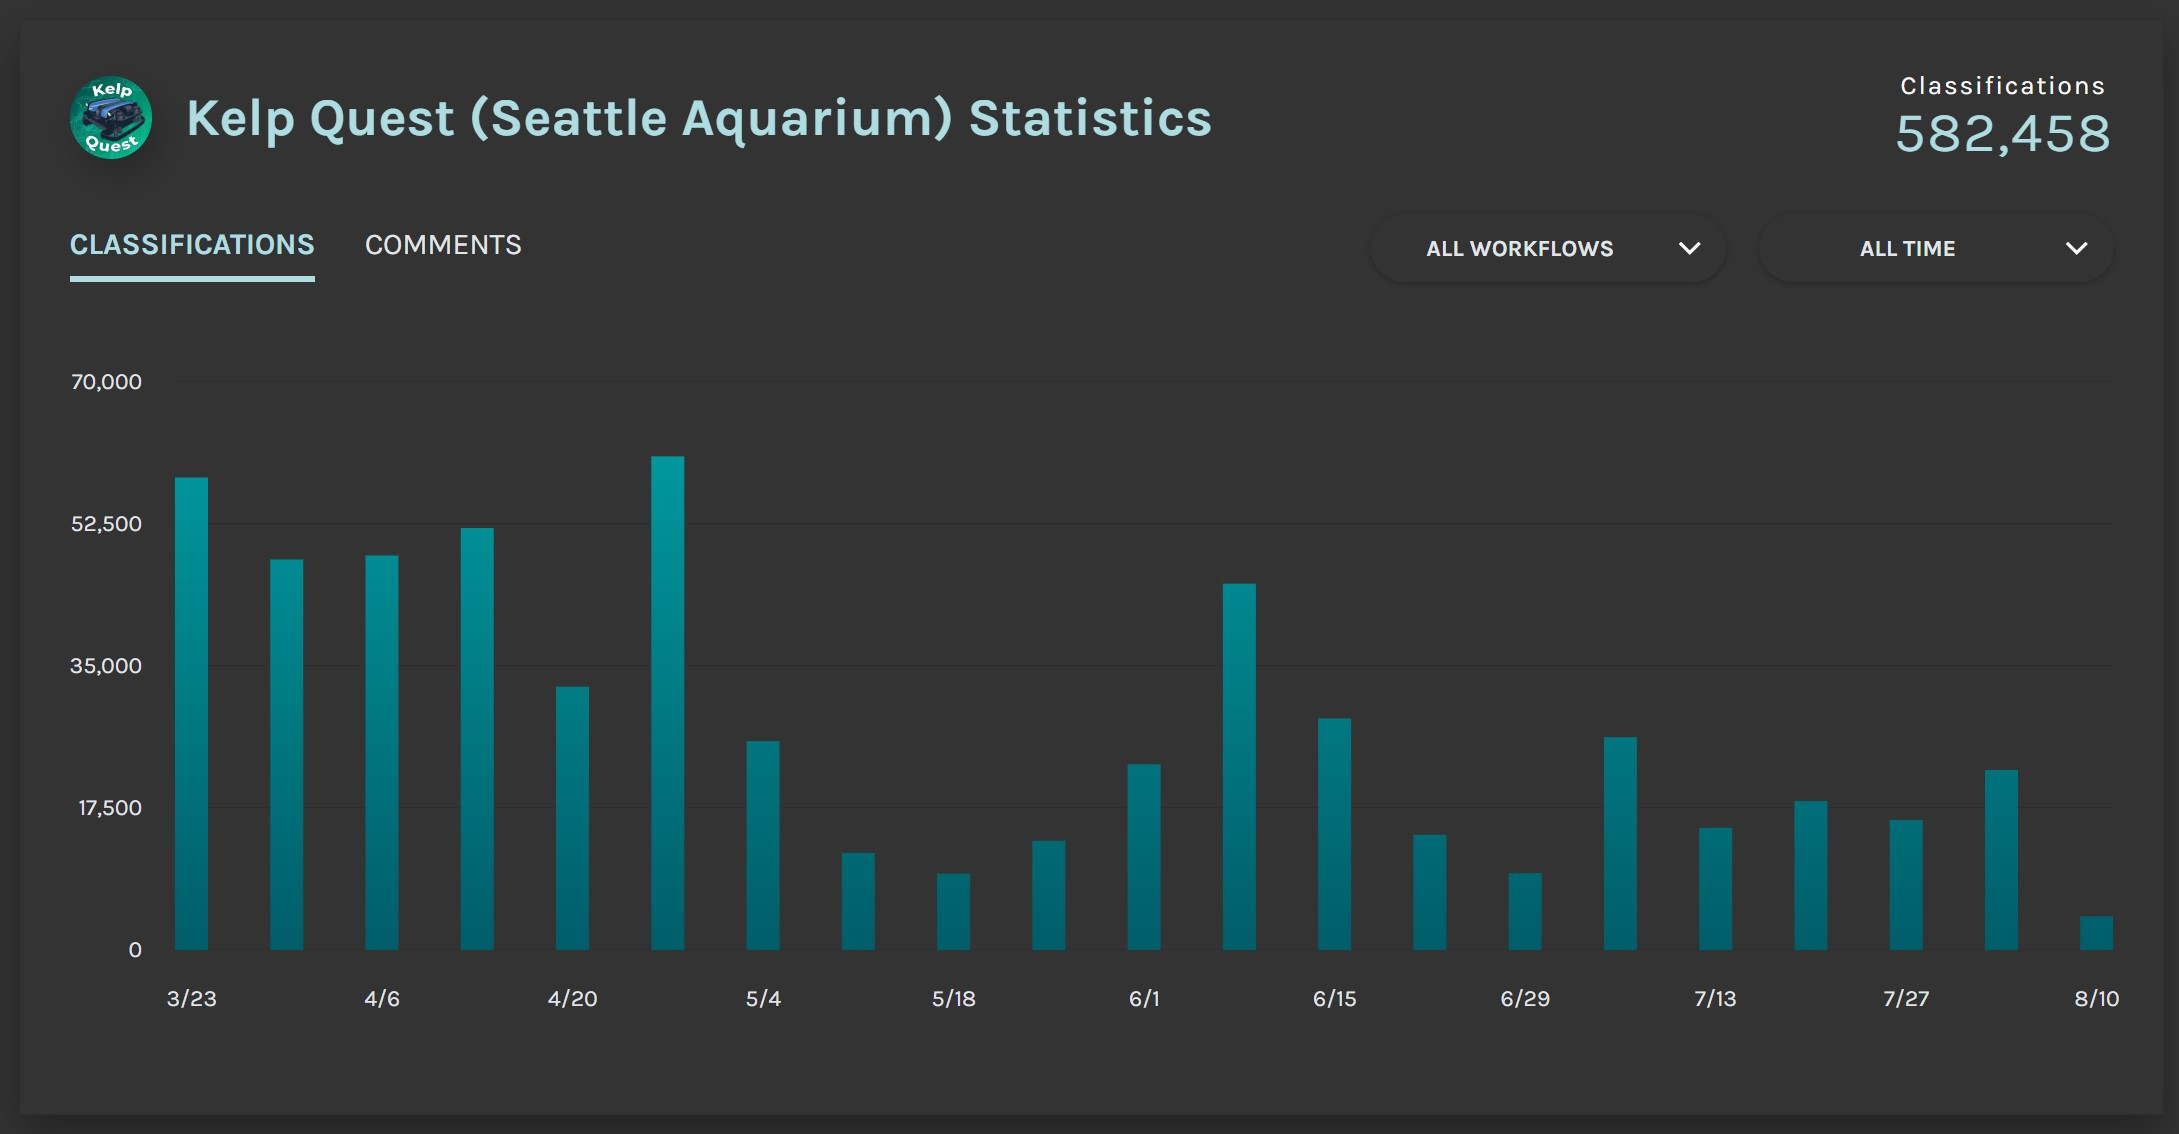
\includegraphics[width=0.98\textwidth]{KelpQuest_classifications.jpg}
\caption{
Weekly Kelp Quest classification volume, all workflows, from project 
launch (March 24, 2026) through August $10^{th}$, 2026. 
582,458 total annotations since March $24^{th}$ equates to --- on average --- 
4160 annotations per day (between launch and August $10^{th}$).  
}
\label{fig:kelpquest_volume}
\end{figure}
\vfil
}

\clearpage

\vbox to \textheight{
\vfil
\begin{table}[H]
\centering
\small
\renewcommand{\arraystretch}{1.08}
\newcommand{\blocksep}{\\[2pt]\hline\noalign{\vskip 3pt}}
\begin{tabular}{l p{13cm}}
\hline
\noalign{\vskip 3pt}
\multicolumn{2}{l}{Final category:
\textbf{\texttt{cover\_red\_algae}}} \\
ROV: & (\texttt{red\_algae\_branching} + \texttt{red\_algae\_bushy}
+ \texttt{red\_algae\_filamentous}
+ \texttt{red\_algae\_flat\_leaf}) \\
Diver: & \texttt{cover\_red\_algae}
\blocksep
\multicolumn{2}{l}{Final category:
\textbf{\texttt{combined\_green\_algae}}} \\
ROV: & \texttt{green\_algae\_ulva} \\
Diver: & (\texttt{cover\_green\_algae} $\cup$
\texttt{superlayer\_green\_algae})
\blocksep
\multicolumn{2}{l}{Final category:
\textbf{\texttt{cover\_crustose\_coralline}}} \\
ROV: & \texttt{red\_algae\_cca} \\
Diver: & \texttt{cover\_crustose\_coralline}
\blocksep
\multicolumn{2}{l}{Final category:
\textbf{\texttt{combined\_substrate\_boulder}}} \\
ROV: & \texttt{boulder} \\
Diver: & (\texttt{substrate\_large\_boulder\_(50cm-1m-wa)}
+ \texttt{substrate\_reef})
\blocksep
\multicolumn{2}{l}{Final category:
\textbf{\texttt{substrate\_rock\_.15.25cm.wa.}}} \\
ROV: & \texttt{cobble} \\
Diver: & \texttt{substrate\_rock\_(15-25cm-wa)}
\blocksep
\multicolumn{2}{l}{Final category:
\textbf{\texttt{combined\_substrate\_pebble}}} \\
ROV: & \texttt{pebble} \\
Diver: & (\texttt{substrate\_pebble\_(0.5-5cm-wa)}
+ \texttt{substrate\_cobble\_(5-15cm-wa)})
\blocksep
\multicolumn{2}{l}{Final category:
\textbf{\texttt{substrate\_shell\_hash}}} \\
ROV: & \texttt{shell\_hash} \\
Diver: & \texttt{substrate\_shell\_hash}
\blocksep
\multicolumn{2}{l}{Final category:
\textbf{\texttt{substrate\_sand}}} \\
ROV: & \texttt{sand\_fine\_shell} \\
Diver: & \texttt{substrate\_sand} \\[2pt]
\hline
\end{tabular}
\caption{
The 8 percent-cover categories directly compared between platforms.
Each block is headed by the category's final name in the combined data, 
followed by the raw category (or categories) from each
platform's own data that were summed, where applicable, to produce it.
``+'' denotes a simple sum of mutually exclusive raw categories;
Diver \texttt{cover\_green\_algae} and 
\texttt{superlayer\_green\_algae} are two independent UPC survey axes 
recorded at the same 30 points, not mutually exclusive outcomes, so a 
simple sum risks double-counting any point where both are present. 
This category instead uses an independence-assumption estimate of the 
union, denoted by $\cup$. 
A similar join was not necessary for the diver's 
\texttt{cover\_red\_algae} and \texttt{superlayer\_red\_algae} due to 
the lack of the latter in the data.
}
\label{tab:combined_categories}
\end{table}
\vfil
}


\clearpage

\vbox to \textheight{
\vfil
\begin{table}[H]
\centering
\begin{tabular}{lll}
\hline
\textbf{Common name} &
\textbf{Diver abundance} &
\textbf{ROV abundance}
\\
\hline
\hline
Ochre/mottled star & 599 & 735 \\
Rock crab & 82 & 158 \\
Burrowing sea cucumber & 110 & 106 \\
Kelp crab & 42 & 44 \\
Leather star & 40 & 46 \\
Plumose anemone & 40 & 42 \\
Green/pallid urchin & 45 & 35 \\
California sea cucumber & 18 & 25 \\
Blood star & 12 & 9 \\
Large anemone & 6 & 6 \\
\hline
\end{tabular}
\caption{
Invertebrate taxa recorded by both diver and ROV survey methods, summed
across all 24 transects (2 sites $\times$ 6 transects $\times$ 2
seasons --- 24 distinct $30 \times 2$ m transects total).
Taxa included ochre/mottled star (\textit{Pisaster ochraceus} and
\textit{Evasterias troschelii});
rock crab (\textit{Cancer productus});
burrowing sea cucumber (\textit{Cucumaria miniata});
kelp crab (\textit{Pugettia producta});
leather star (\textit{Dermasterias imbricata});
plumose anemone (\textit{Metridium farcimen});
green/pallid urchin (\textit{Strongylocentrotus droebachiensis} and
\textit{Strongylocentrotus pallidus});
California sea cucumber (\textit{Apostichopus californicus});
blood star (\textit{Henricia leviuscula});
and large anemone (\textit{Urticina} spp.).
}
\label{tab:abundances}
\end{table}
\vfil
}

\clearpage

\vbox to \textheight{
\vfil
\begin{table}[H]
\centering
\begin{tabular}{llll}
\hline
Taxon &
Rate ratio &
$p$-value &
Converged
\\
\hline
\hline
Ochre/mottled star & 1.18 & $0.180$ & Yes \\
Rock crab & 1.47 & $0.347$ & No \\
Burrowing sea cucumber & 1.20 & $6.2 \times 10^{-38}$ & No \\
Kelp crab & 1.18 & $0.661$ & Yes \\
Leather star & 1.17 & $0.552$ & Yes \\
Plumose anemone & 1.16 & $0.675$ & Yes \\
Green/pallid urchin & 1.29 & $0.756$ & No \\
California sea cucumber & 1.41 & $0.291$ & Yes \\
Blood star & 0.75 & $0.514$ & No \\
Large anemone & 1.12 & $0.877$ & Yes \\
\hline
\end{tabular}
\caption{
Negative binomial GLMM results for all 10 overlapping abundance taxa under the
full mixed-effects specification (\texttt{count} $\sim$ type + site +
season + depth + $(1|\text{transect\_id})$).
This table is deliberately not the one to interpret --- \tabref{tab:abundance_models}
reports the final, per-taxon best estimates and is the basis for every
abundance result discussed in the text.
Its purpose is to make visible what those final estimates were selected
from: for the four taxa whose mixed models did not converge, this is the
only place the discarded mixed-model estimates appear, and comparing them
against their simplified counterparts in \tabref{tab:abundance_models} is what
shows the refits to be a numerical necessity rather than a convenient choice
of specification.
Rate ratios are ROV relative to a diver reference level.
``No'' under Converged indicates the model returned a fit but raised
convergence warnings (degenerate Hessian, near-unidentifiability, or
iteration-limit warnings);
these four estimates, and in particular burrowing sea cucumber's implausibly
small $p$-value, likely reflect optimizer instability from the small sample
size (12 transects) rather than genuine effects, and should not be interpreted
at face value.
}
\label{tab:abundance_all_models_full_mixed}
\end{table}
\vfil
}

\clearpage

\vbox to \textheight{
\vfil
\begin{table}[H]
\centering
% 7 columns at the default 6pt inter-column padding runs ~15pt past the text
% block; 4pt brings it back inside, matching the correlation tables below
\setlength{\tabcolsep}{4pt}
\begin{tabular}{lllllll}
\hline
Taxon &
Diver total &
ROV total &
Model &
Rate ratio &
$p$-value &
Converged
\\
\hline
\hline
Ochre/mottled star & 599 & 735 & Mixed & 1.18 & $0.180$ & Yes \\
Rock crab & 82 & 158 & Simplified & 1.51 & $0.386$ & No$^{a}$ \\
Burrowing sea cucumber & 110 & 106 & Simplified & 1.22 & $0.612$ & Yes 
\\
Kelp crab & 42 & 44 & Mixed & 1.18 & $0.661$ & Yes \\
Leather star & 40 & 46 & Mixed & 1.17 & $0.552$ & Yes \\
Plumose anemone & 40 & 42 & Mixed & 1.16 & $0.675$ & Yes \\
Green/pallid urchin & 45 & 35 & Simplified & 1.36 & $0.682$ & No$^{b}$ 
\\
California sea cucumber & 18 & 25 & Mixed & 1.41 & $0.291$ & Yes \\
Blood star & 12 & 9 & Simplified & 0.75 & $0.514$ & No$^{c}$ \\
Large anemone & 6 & 6 & Mixed & 1.12 & $0.877$ & Yes \\
\hline
\end{tabular}
\caption{
Negative binomial GLMM results for all 10 overlapping abundance taxa. 
``Mixed'' models include a $(1|\text{transect\_id})$ random intercept 
(\texttt{count} $\sim$ type + site + season + depth + 
$(1|\text{transect\_id})$); ``Simplified'' models drop the random 
intercept (\texttt{count} $\sim$ type + site + season + depth) after 
the mixed-model version failed to converge, trading proper handling of 
the repeated-measures (summer/winter) structure for numerical 
stability. Diver and ROV totals are summed raw counts across all 24 
transects. Rate ratios are ROV relative to a diver reference level. See 
notes below for the three taxa still flagged after simplification.
}
\label{tab:abundance_models}
\end{table}
\bigskip
\noindent\textbf{Notes:}
\begin{itemize}
\item[$^{a}$] Rock crab (simplified model): ``alternation limit reached'' 
-- the dispersion parameter did not stabilize even without the random 
intercept, plausibly driven by the single large outlier transect 
(Centennial Park, winter, transect 1: 62 diver / 130 ROV, an order of 
magnitude above every other transect).
\item[$^{b}$] Green/pallid urchin (simplified model): ``glm.fit: fitted 
rates numerically 0 occurred'' -- consistent with this taxon's abundance 
being concentrated in a small number of transects (predominantly Elliott 
Bay Marina, shallow, summer) with near-zero counts elsewhere.
\item[$^{c}$] Blood star (simplified model): ``iteration limit reached'' 
(twice) -- likely reflects this taxon's low overall abundance (12 diver, 9 
ROV across all 24 transects), leaving too little information to estimate 
the dispersion parameter precisely.
\end{itemize}
\vfil
}

\clearpage

\vbox to \textheight{
\vfil
\begin{figure}[H]
\centering

\includegraphics[width=0.98\textwidth]{abundance_head-to-head.pdf}
\caption{
Diver- versus ROV-recorded abundance (individual counts) for each of 
the 10
invertebrate taxa compared in this study, one point per transect ($n=24$
transects per panel).
Panels are labeled (a)--(j); axis scales are set independently per 
taxon to
accommodate their differing abundance ranges.
The dashed line marks 1:1 agreement between platforms: points below the
line
indicate transects where the ROV recorded fewer individuals than
divers, and
points above indicate the ROV recorded more.
Each panel is annotated with that taxon's Pearson correlation between the two
platforms across the 24 transects; note that these describe agreement in
pattern, and are independent of the vertical offset from the 1:1 line,
which describes agreement in level.
Rock crab's $r=1.00$ (panel b) rests entirely on the single high-count
transect visible in that panel and should not be read as strong agreement ---
see \tabref{tab:cor_abundance} and its notes.
See \tabref{tab:abundance_models} for corresponding model results, and
\tabref{tab:cor_abundance} for confidence intervals, $p$-values, and
Spearman's $\rho$ accompanying each panel's $r$.
}
\label{fig:abundance_head-to-head}
\end{figure}
\vfil
}

\clearpage

\vbox to \textheight{
\vfil
\begin{table}[H]
\centering
\begin{tabular}{llll}
\hline
Category &
Odds ratio &
$p$-value &
Converged
\\
\hline
\hline
Red algae cover & 0.73 & $0.062$ & Yes \\
Green algae cover & 0.92 & $0.705$ & Yes \\
Crustose coralline algae (CCA) & 0.29 & $5.5 \times 10^{-12}$ & Yes \\
Boulder substrate & 0.18 & $1.8 \times 10^{-7}$ & Yes \\
Rock, 15--25\,cm (``cobble'') substrate & 1.12 & $0.809$ & Yes \\
Pebble substrate & 0.36 & $3.8 \times 10^{-7}$ & Yes \\
Sand substrate & 0.36 & $9.1 \times 10^{-4}$ & Yes \\
Shell hash substrate & 0.04 & $1.3 \times 10^{-19}$ & Yes \\
\hline
\end{tabular}
\caption{
Beta-binomial GLMM results for all 8 percent-cover categories. 
Odds ratios are ROV relative to a diver reference level; values below 1 
indicate the ROV recorded that category at lower odds than divers. 
All 8 models converged without warnings.
}
\label{tab:pc_all_models}
\end{table}
\vfil
}

\clearpage

\vbox to \textheight{
\vfil
\begin{table}[H]
\centering

\begin{tabular}{llll}
\hline
Category &
Odds ratio  &
$p$-value &
Converged
\\
\hline
\hline
Crustose coralline algae (CCA) & 0.31 & $1.4 \times 10^{-6}$ & Yes \\
Boulder substrate & 0.32 & $2.7 \times 10^{-4}$ & Yes \\
Rock, 15--25\,cm (``cobble'') substrate & 1.30 & $0.631$ & Yes \\
Pebble substrate & 0.64 & $0.069$ & Yes \\
Sand substrate & 0.60 & $0.299$ & Yes \\
Shell hash substrate & 0.03 & $3.6 \times 10^{-16}$ & Yes \\
\hline
\end{tabular}
\caption{
Beta-binomial GLMM results restricted to winter transects only, for CCA 
and the 5 substrate categories with \texttt{season} dropped, as no season 
variation remains once restricted to winter). 
Odds ratios are ROV relative to a diver reference level. 
All 6 models converged without warnings.
}
\label{tab:pc_winter_substrate}
\end{table}
\vfil
}

\clearpage

\vbox to \textheight{
\vfil
\begin{figure}[H]
\centering
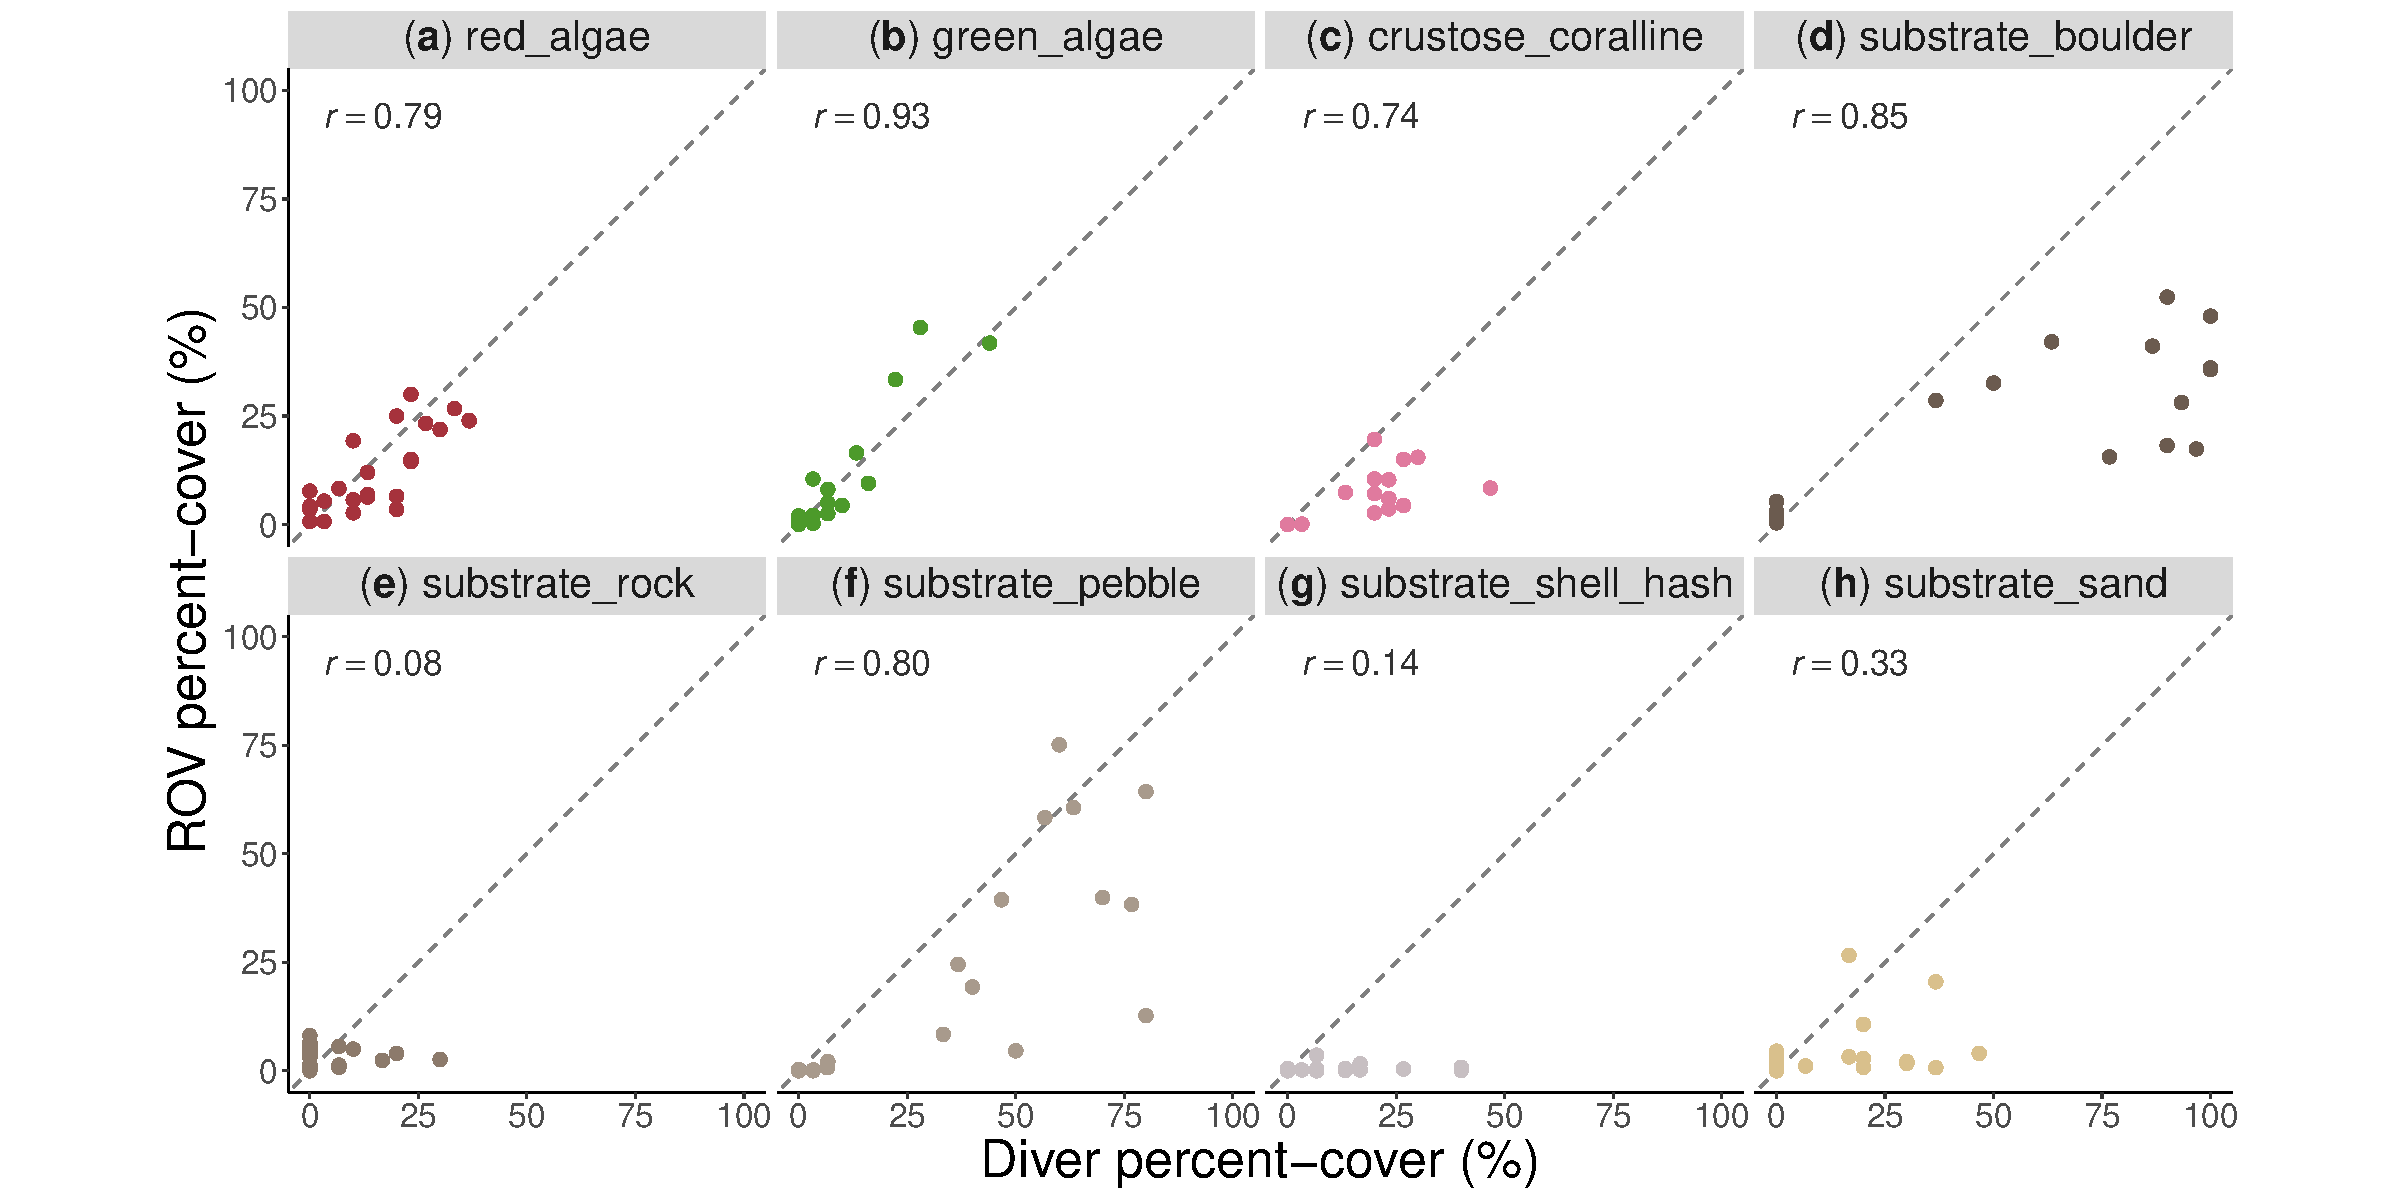
\includegraphics[width=0.98\textwidth]{percent-cover_head-to-head.pdf}
\caption{
Diver- versus ROV-recorded percent-cover for each of the 8 categories compared
in this study (\tabref{tab:combined_categories}), one point per transect
$\times$ season ($n=24$).
Panels are labeled (a)--(h) and ordered as red algae, green algae, and crustose
coralline algae (a--c), followed by the five substrate categories in order of
decreasing grain size --- boulder, rock ($15$--$25~cm$, ``cobble''), pebble,
shell hash, and sand (d--h).
All panels share fixed 0--100\% axes.
The dashed line marks 1:1 agreement between platforms; points falling below
the line indicate transects where the ROV recorded lower percent-cover than
divers for that category.
Each panel is annotated with that category's Pearson correlation between the
two platforms across the 24 transects.
Panels (d) and (e) illustrate the report's central point about these two
quantities being separable: boulder sits far below the 1:1 line yet is
tightly correlated ($r=0.85$), while cobble straddles the line yet is not
correlated at all ($r=0.08$).
See \tabref{tab:pc_all_models} for corresponding model results, and
\tabref{tab:cor_pc_all} for confidence intervals, $p$-values, and Spearman's
$\rho$ accompanying each panel's $r$.
}
\label{fig:percent-cover_head-to-head}
\end{figure}
\vfil
}

\clearpage

\vbox to \textheight{
\vfil
\begin{figure}[H]
\centering
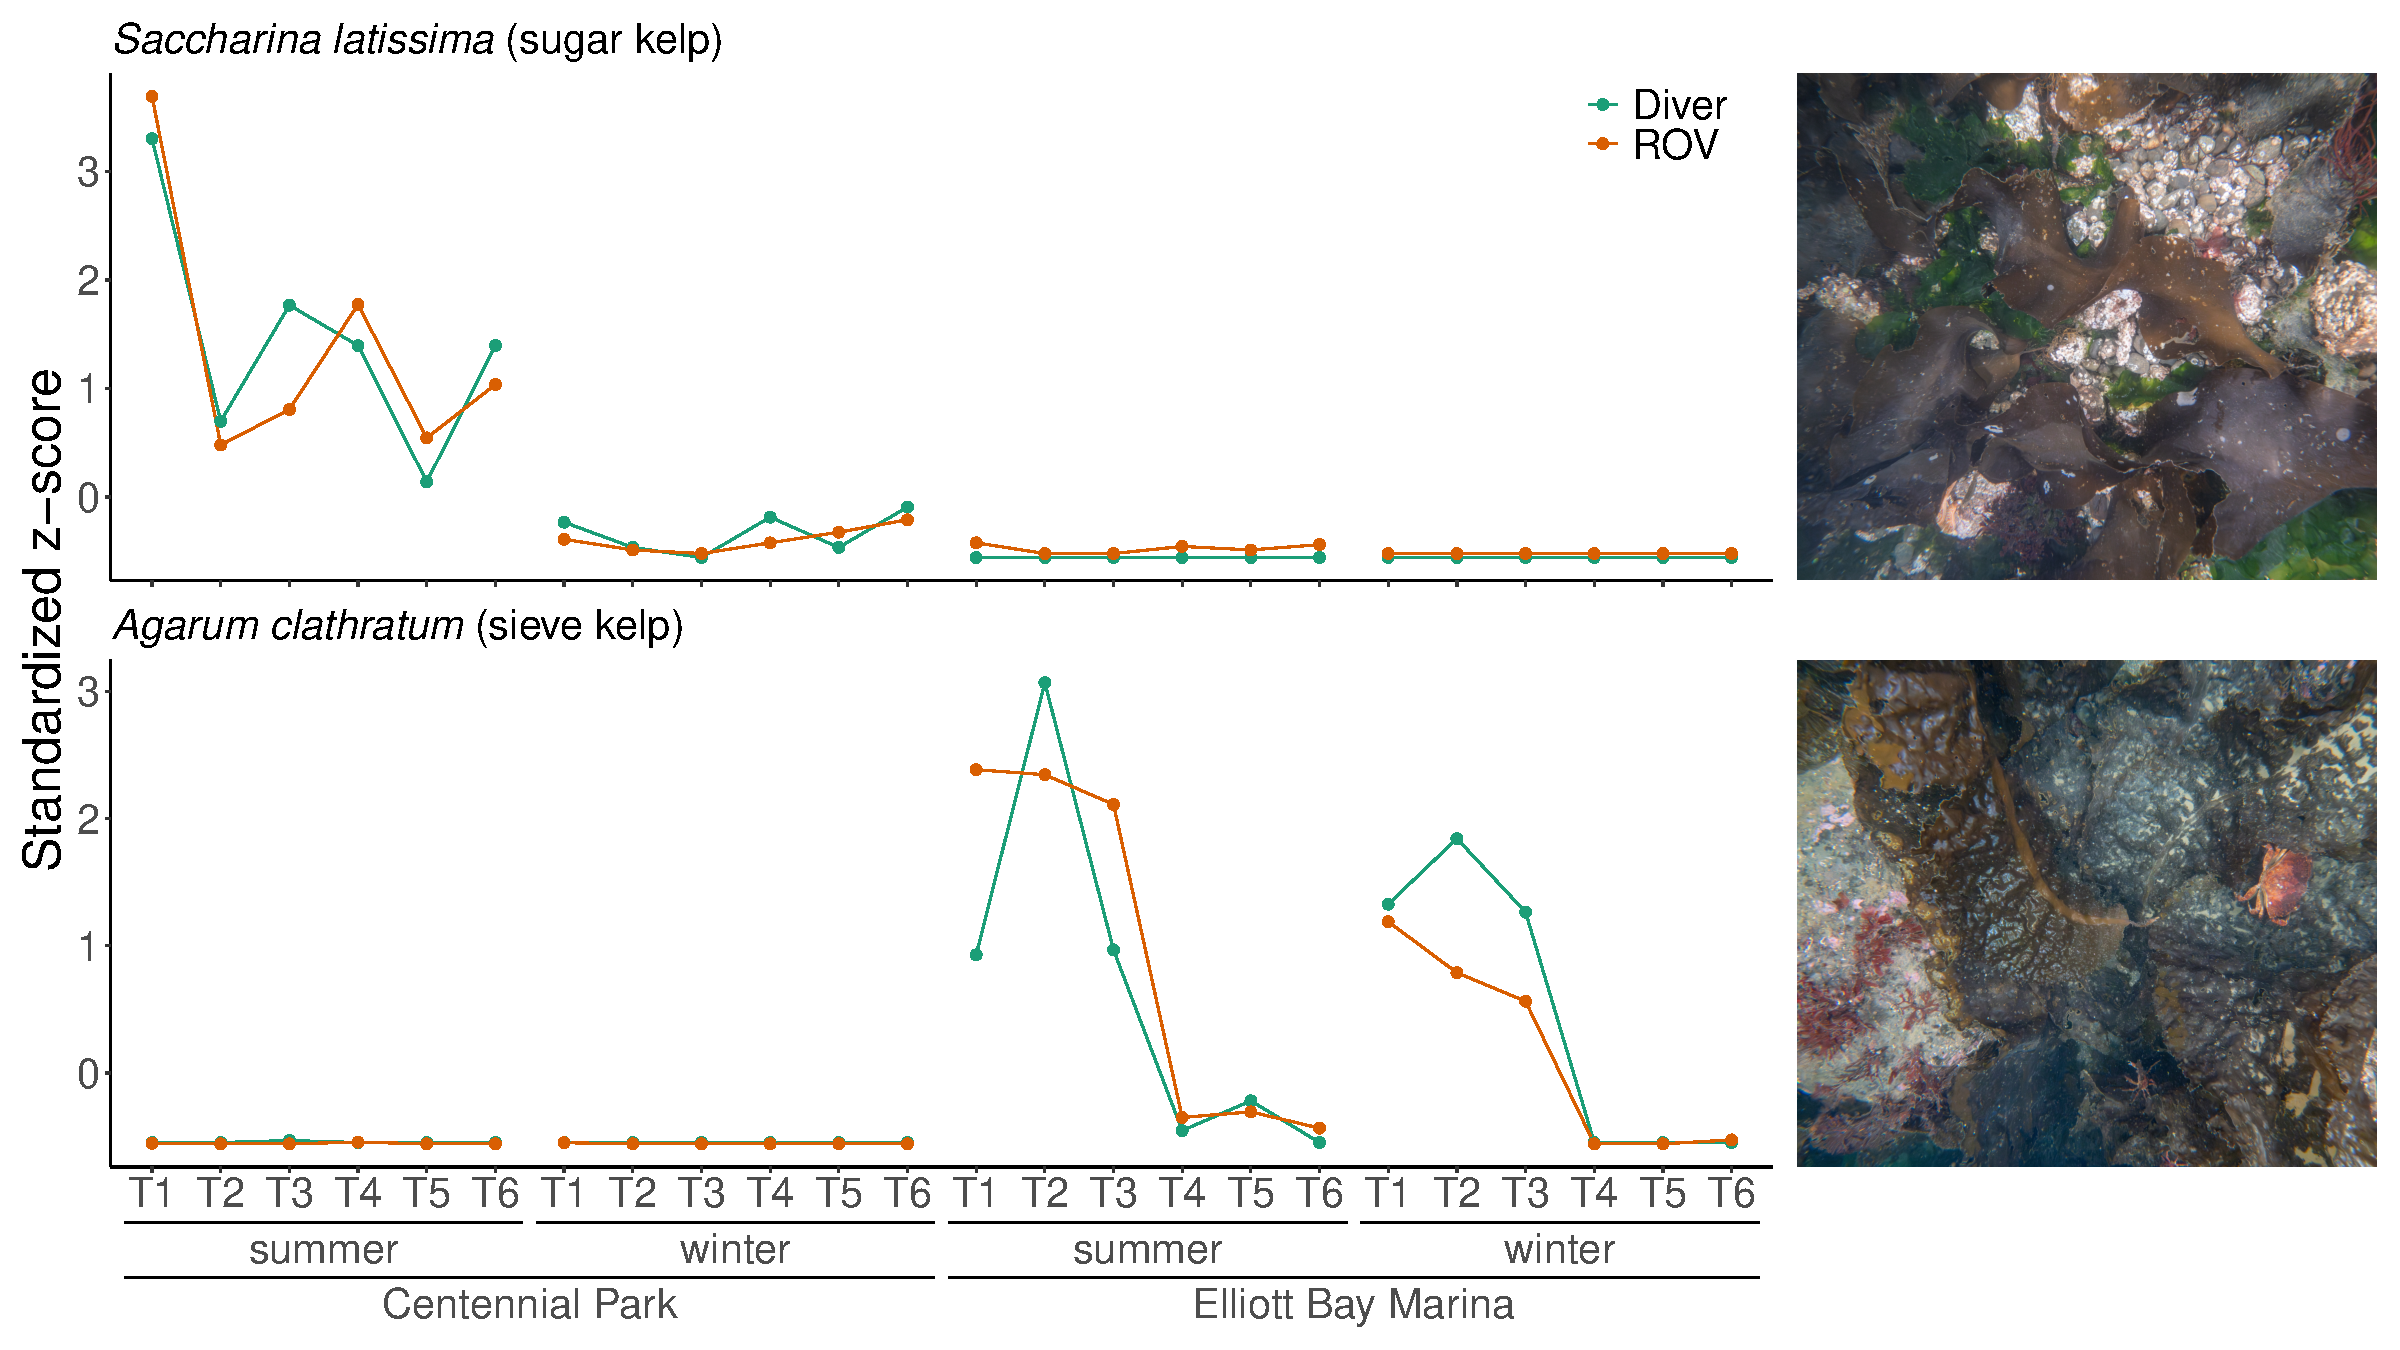
\includegraphics[width=0.98\textwidth]{z-scores.pdf}
\caption{
Standardized (z-scored) diver density and ROV percent-cover for 
\textit{Saccharina latissima} (sugar kelp, top) and \textit{Agarum
clathratum} (sieve kelp, bottom) across all 24 site $\times$ transect $\times$ 
season combinations, grouped by site, season, and transect (1--6) along the 
x-axis.
Pearson's correlation coefficient for the two z-scores were very strongly 
correlated for \textit{Saccharina} ($r=0.96$, $p=6.3\times10^{-14}$), and 
\textit{Agarum} ($r=0.88$, $p=1.7\times10^{-8}$), indicating that both the ROV 
and the diver methods --- despite capturing mathematically distinct 
observations --- capture statistically indistinguishable kelp metrics.
Representative ROV photographs of each species are shown at right (top:
sugar kelp; bottom: sieve kelp).
}
\label{fig:z-scores}
\end{figure}
\vfil
}


\clearpage

\vbox to \textheight{
\vfil
\begin{table}[H]
\centering
\small
\setlength{\tabcolsep}{4pt}
\begin{tabular}{lllllll}
\hline
Category &
$n$ &
Pearson $r$ &
95\% CI &
$p$-value &
Spearman $\rho$ &
$p$-value
\\
\hline
\hline
Red algae cover & 24 & 0.79 & 0.57, 0.91 & $4.2 \times 10^{-6}$ & 0.76 & $1.4 \times 10^{-5}$ \\
Green algae cover & 24 & 0.93 & 0.85, 0.97 & $3.5 \times 10^{-11}$ & 0.90 & $1.3 \times 10^{-9}$ \\
Crustose coralline algae (CCA) & 24 & 0.74 & 0.48, 0.88 & $3.8 \times 10^{-5}$ & 0.88 & $9.4 \times 10^{-9}$ \\
Boulder substrate & 24 & 0.85 & 0.68, 0.93 & $1.3 \times 10^{-7}$ & 0.82 & $7.1 \times 10^{-7}$ \\
Rock, 15--25\,cm (``cobble'') substrate & 24 & 0.08 & -0.34, 0.47 & $0.723$ & 0.19 & $0.383$ \\
Pebble substrate & 24 & 0.80 & 0.59, 0.91 & $2.5 \times 10^{-6}$ & 0.87 & $2.4 \times 10^{-8}$ \\
Sand substrate & 24 & 0.33 & -0.08, 0.65 & $0.113$ & 0.32 & $0.122$ \\
Shell hash substrate & 24 & 0.14 & -0.28, 0.51 & $0.513$ & 0.46 & $0.024$ \\
\hline
\end{tabular}
\caption{
ROV--diver correlations for all 8 percent-cover categories, across all $n=24$
site $\times$ transect $\times$ season combinations.
Pearson $r$ is computed on the paired transect-averaged proportions; because
standardization is a linear transformation, these values are identical to the
correlations between the two platforms' z-scored series
(\tabref{tab:cor_zscore_pc}).
Spearman's $\rho$ repeats the test on ranks alone, and is reported alongside
because several of these categories are dominated by a small number of
transects, to which Pearson's $r$ is far more sensitive than $\rho$.
Note that these correlations and the odds ratios of \tabref{tab:pc_all_models}
answer different questions and need not agree: boulder, for example, shows a
large and highly significant level difference between platforms
($\mathrm{OR}=0.18$) while tracking diver-recorded cover closely across
transects ($r=0.85$).
}
\label{tab:cor_pc_all}
\end{table}
\vfil
}


\clearpage

\vbox to \textheight{
\vfil
\begin{table}[H]
\centering
\small
\setlength{\tabcolsep}{4pt}
\begin{tabular}{lllllll}
\hline
Category &
$n$ &
Pearson $r$ &
95\% CI &
$p$-value &
Spearman $\rho$ &
$p$-value
\\
\hline
\hline
Crustose coralline algae (CCA) & 12 & 0.69 & 0.18, 0.90 & $0.014$ & 0.82 & $9.9 \times 10^{-4}$ \\
Boulder substrate & 12 & 0.93 & 0.76, 0.98 & $1.2 \times 10^{-5}$ & 0.85 & $5.0 \times 10^{-4}$ \\
Rock, 15--25\,cm (``cobble'') substrate & 12 & -0.17 & -0.68, 0.45 & $0.592$ & -0.08 & $0.810$ \\
Pebble substrate & 12 & 0.95 & 0.84, 0.99 & $1.5 \times 10^{-6}$ & 0.96 & $9.9 \times 10^{-7}$ \\
Sand substrate & 12 & 0.33 & -0.30, 0.76 & $0.292$ & 0.35 & $0.260$ \\
Shell hash substrate & 12 & -0.13 & -0.65, 0.48 & $0.695$ & 0.13 & $0.685$ \\
\hline
\end{tabular}
\caption{
ROV--diver correlations restricted to the $n=12$ winter transects, for CCA and
the 5 substrate categories --- the same restriction applied to the
beta-binomial models in \tabref{tab:pc_winter_substrate}.
Columns as in \tabref{tab:cor_pc_all}.
}
\label{tab:cor_pc_winter}
\end{table}
\vfil
}


\clearpage

\vbox to \textheight{
\vfil
\begin{table}[H]
\centering
\small
\setlength{\tabcolsep}{4pt}
\begin{tabular}{lllllll}
\hline
Category &
$n$ &
Pearson $r$ &
95\% CI &
$p$-value &
Spearman $\rho$ &
$p$-value
\\
\hline
\hline
Ochre/mottled star & 24 & 0.70 & 0.42, 0.86 & $1.2 \times 10^{-4}$ & 0.54 & $0.006$ \\
Rock crab & 24 & 1.00 & 0.99, 1.00 & $8.2 \times 10^{-27}$ & 0.37 & $0.072$ \\
Burrowing sea cucumber & 24 & 0.96 & 0.90, 0.98 & $2.3 \times 10^{-13}$ & 0.73 & $4.9 \times 10^{-5}$ \\
Kelp crab & 24 & 0.23 & -0.19, 0.58 & $0.282$ & 0.35 & $0.095$ \\
Leather star & 24 & 0.54 & 0.18, 0.78 & $0.006$ & 0.77 & $1.3 \times 10^{-5}$ \\
Plumose anemone & 24 & 0.49 & 0.11, 0.75 & $0.014$ & 0.84 & $2.6 \times 10^{-7}$ \\
Green/pallid urchin & 24 & 0.69 & 0.40, 0.86 & $1.9 \times 10^{-4}$ & 0.65 & $6.2 \times 10^{-4}$ \\
California sea cucumber & 24 & 0.70 & 0.42, 0.86 & $1.2 \times 10^{-4}$ & 0.81 & $1.9 \times 10^{-6}$ \\
Blood star & 24 & 0.40 & -0.01, 0.69 & $0.054$ & 0.56 & $0.004$ \\
Large anemone & 24 & 0.28 & -0.14, 0.61 & $0.189$ & 0.40 & $0.054$ \\
\hline
\end{tabular}
\caption{
ROV--diver correlations for all 10 overlapping abundance taxa, across all
$n=24$ site $\times$ transect $\times$ season combinations, computed on raw
transect totals (the same quantity plotted in
\figref{fig:abundance_head-to-head}).
Columns as in \tabref{tab:cor_pc_all}.
Rock crab's $r=1.00$ is an artifact of the single Centennial Park winter
transect 1 outlier (62 diver / 130 ROV) discussed in the \textit{Results}:
all 23 other transects fall between 0 and 3
individuals for both platforms, and excluding that one transect drops the
correlation to $r=0.25$ ($p=0.243$). Spearman's $\rho$, insensitive to the
outlier's magnitude, independently flags this ($\rho=0.37$, $p=0.072$).
}
\label{tab:cor_abundance}
\end{table}
\vfil
}


\clearpage

\vbox to \textheight{
\vfil
\begin{table}[H]
\centering
\small
\begin{tabular}{llllll}
\hline
Category &
$n$ &
Pearson $r$ &
$p$-value &
Mean $|\Delta z|$ &
Max $|\Delta z|$
\\
\hline
\hline
\multicolumn{6}{l}{\textit{percent-cover, all seasons}} \\
Red algae cover & 24 & 0.79 & $4.2 \times 10^{-6}$ & 0.52 & 1.31 \\
Green algae cover & 24 & 0.93 & $3.5 \times 10^{-11}$ & 0.24 & 0.90 \\
Crustose coralline algae (CCA) & 24 & 0.74 & $3.8 \times 10^{-5}$ & 0.47 & 1.97 \\
Boulder substrate & 24 & 0.85 & $1.3 \times 10^{-7}$ & 0.37 & 1.26 \\
Rock, 15--25\,cm (``cobble'') substrate & 24 & 0.08 & $0.723$ & 1.06 & 3.37 \\
Pebble substrate & 24 & 0.80 & $2.5 \times 10^{-6}$ & 0.43 & 1.87 \\
Sand substrate & 24 & 0.33 & $0.113$ & 0.83 & 3.16 \\
Shell hash substrate & 24 & 0.14 & $0.513$ & 0.81 & 4.37 \\
\hline
\textbf{All 8 series pooled (standardized)} & 192 & 0.58 & $7.1 \times 10^{-19}$ & 0.59 & --- \\
\noalign{\vskip 3pt}
\multicolumn{6}{l}{\textit{percent-cover, winter only}} \\
Crustose coralline algae (CCA) & 12 & 0.69 & $0.014$ & 0.44 & 1.82 \\
Boulder substrate & 12 & 0.93 & $1.2 \times 10^{-5}$ & 0.25 & 1.00 \\
Rock, 15--25\,cm (``cobble'') substrate & 12 & -0.17 & $0.592$ & 1.21 & 2.91 \\
Pebble substrate & 12 & 0.95 & $1.5 \times 10^{-6}$ & 0.21 & 0.65 \\
Sand substrate & 12 & 0.33 & $0.292$ & 0.78 & 2.24 \\
Shell hash substrate & 12 & -0.13 & $0.695$ & 1.02 & 3.57 \\
\hline
\textbf{All 6 series pooled (standardized)} & 72 & 0.43 & $1.4 \times 10^{-4}$ & 0.65 & --- \\
\hline
\end{tabular}
\caption{
Z-score summary for the percent-cover categories.
Each platform's series is standardized against its own mean and standard
deviation, placing the two on one shared, unitless axis
(Eqn.~\ref{eq:z-score}).
The Pearson $r$ column is identical to that of \tabref{tab:cor_pc_all} and
\tabref{tab:cor_pc_winter} --- standardization is a linear transformation and
$r$ is invariant to it --- and is repeated here only so each row can be read
against the two columns that standardization does make available.
Mean and max $|\Delta z|$ are the average and worst per-transect gap between
the two platforms' standardized values, in standard deviations; unlike $r$,
these are on an interpretable ``how far apart were the two platforms on a
given transect'' scale.
The pooled row stacks every standardized series in its block into a single
series and correlates once, giving one overall agreement statistic per block
(equal, with equal $n$ per series, to the unweighted mean of that block's
per-category $r$).
}
\label{tab:cor_zscore_pc}
\end{table}
\vfil
}


\clearpage

\vbox to \textheight{
\vfil
\begin{table}[H]
\centering
\small
\begin{tabular}{llllll}
\hline
Category &
$n$ &
Pearson $r$ &
$p$-value &
Mean $|\Delta z|$ &
Max $|\Delta z|$
\\
\hline
\hline
Ochre/mottled star & 24 & 0.70 & $1.2 \times 10^{-4}$ & 0.59 & 1.68 \\
Rock crab & 24 & 1.00 & $8.2 \times 10^{-27}$ & 0.05 & 0.14 \\
Burrowing sea cucumber & 24 & 0.96 & $2.3 \times 10^{-13}$ & 0.21 & 0.91 \\
Kelp crab & 24 & 0.23 & $0.282$ & 0.85 & 3.87 \\
Leather star & 24 & 0.54 & $0.006$ & 0.48 & 3.19 \\
Plumose anemone & 24 & 0.49 & $0.014$ & 0.45 & 3.63 \\
Green/pallid urchin & 24 & 0.69 & $1.9 \times 10^{-4}$ & 0.44 & 2.84 \\
California sea cucumber & 24 & 0.70 & $1.2 \times 10^{-4}$ & 0.41 & 1.90 \\
Blood star & 24 & 0.40 & $0.054$ & 0.58 & 4.05 \\
Large anemone & 24 & 0.28 & $0.189$ & 0.63 & 3.63 \\
\hline
\textbf{All 10 series pooled (standardized)} & 240 & 0.60 & $7.9 \times 10^{-25}$ & 0.47 & --- \\
\hline
\end{tabular}
\caption{
Z-score summary for the 10 abundance taxa.
Columns and the pooled row as in \tabref{tab:cor_zscore_pc}.
Rock crab's mean $|\Delta z|$ of 0.05 is the same single-outlier artifact
noted in \tabref{tab:cor_abundance}, not exceptional agreement.
}
\label{tab:cor_zscore_abundance}
\end{table}
\vfil
}


\clearpage

\vbox to \textheight{
\vfil
\begin{figure}[H]
\centering
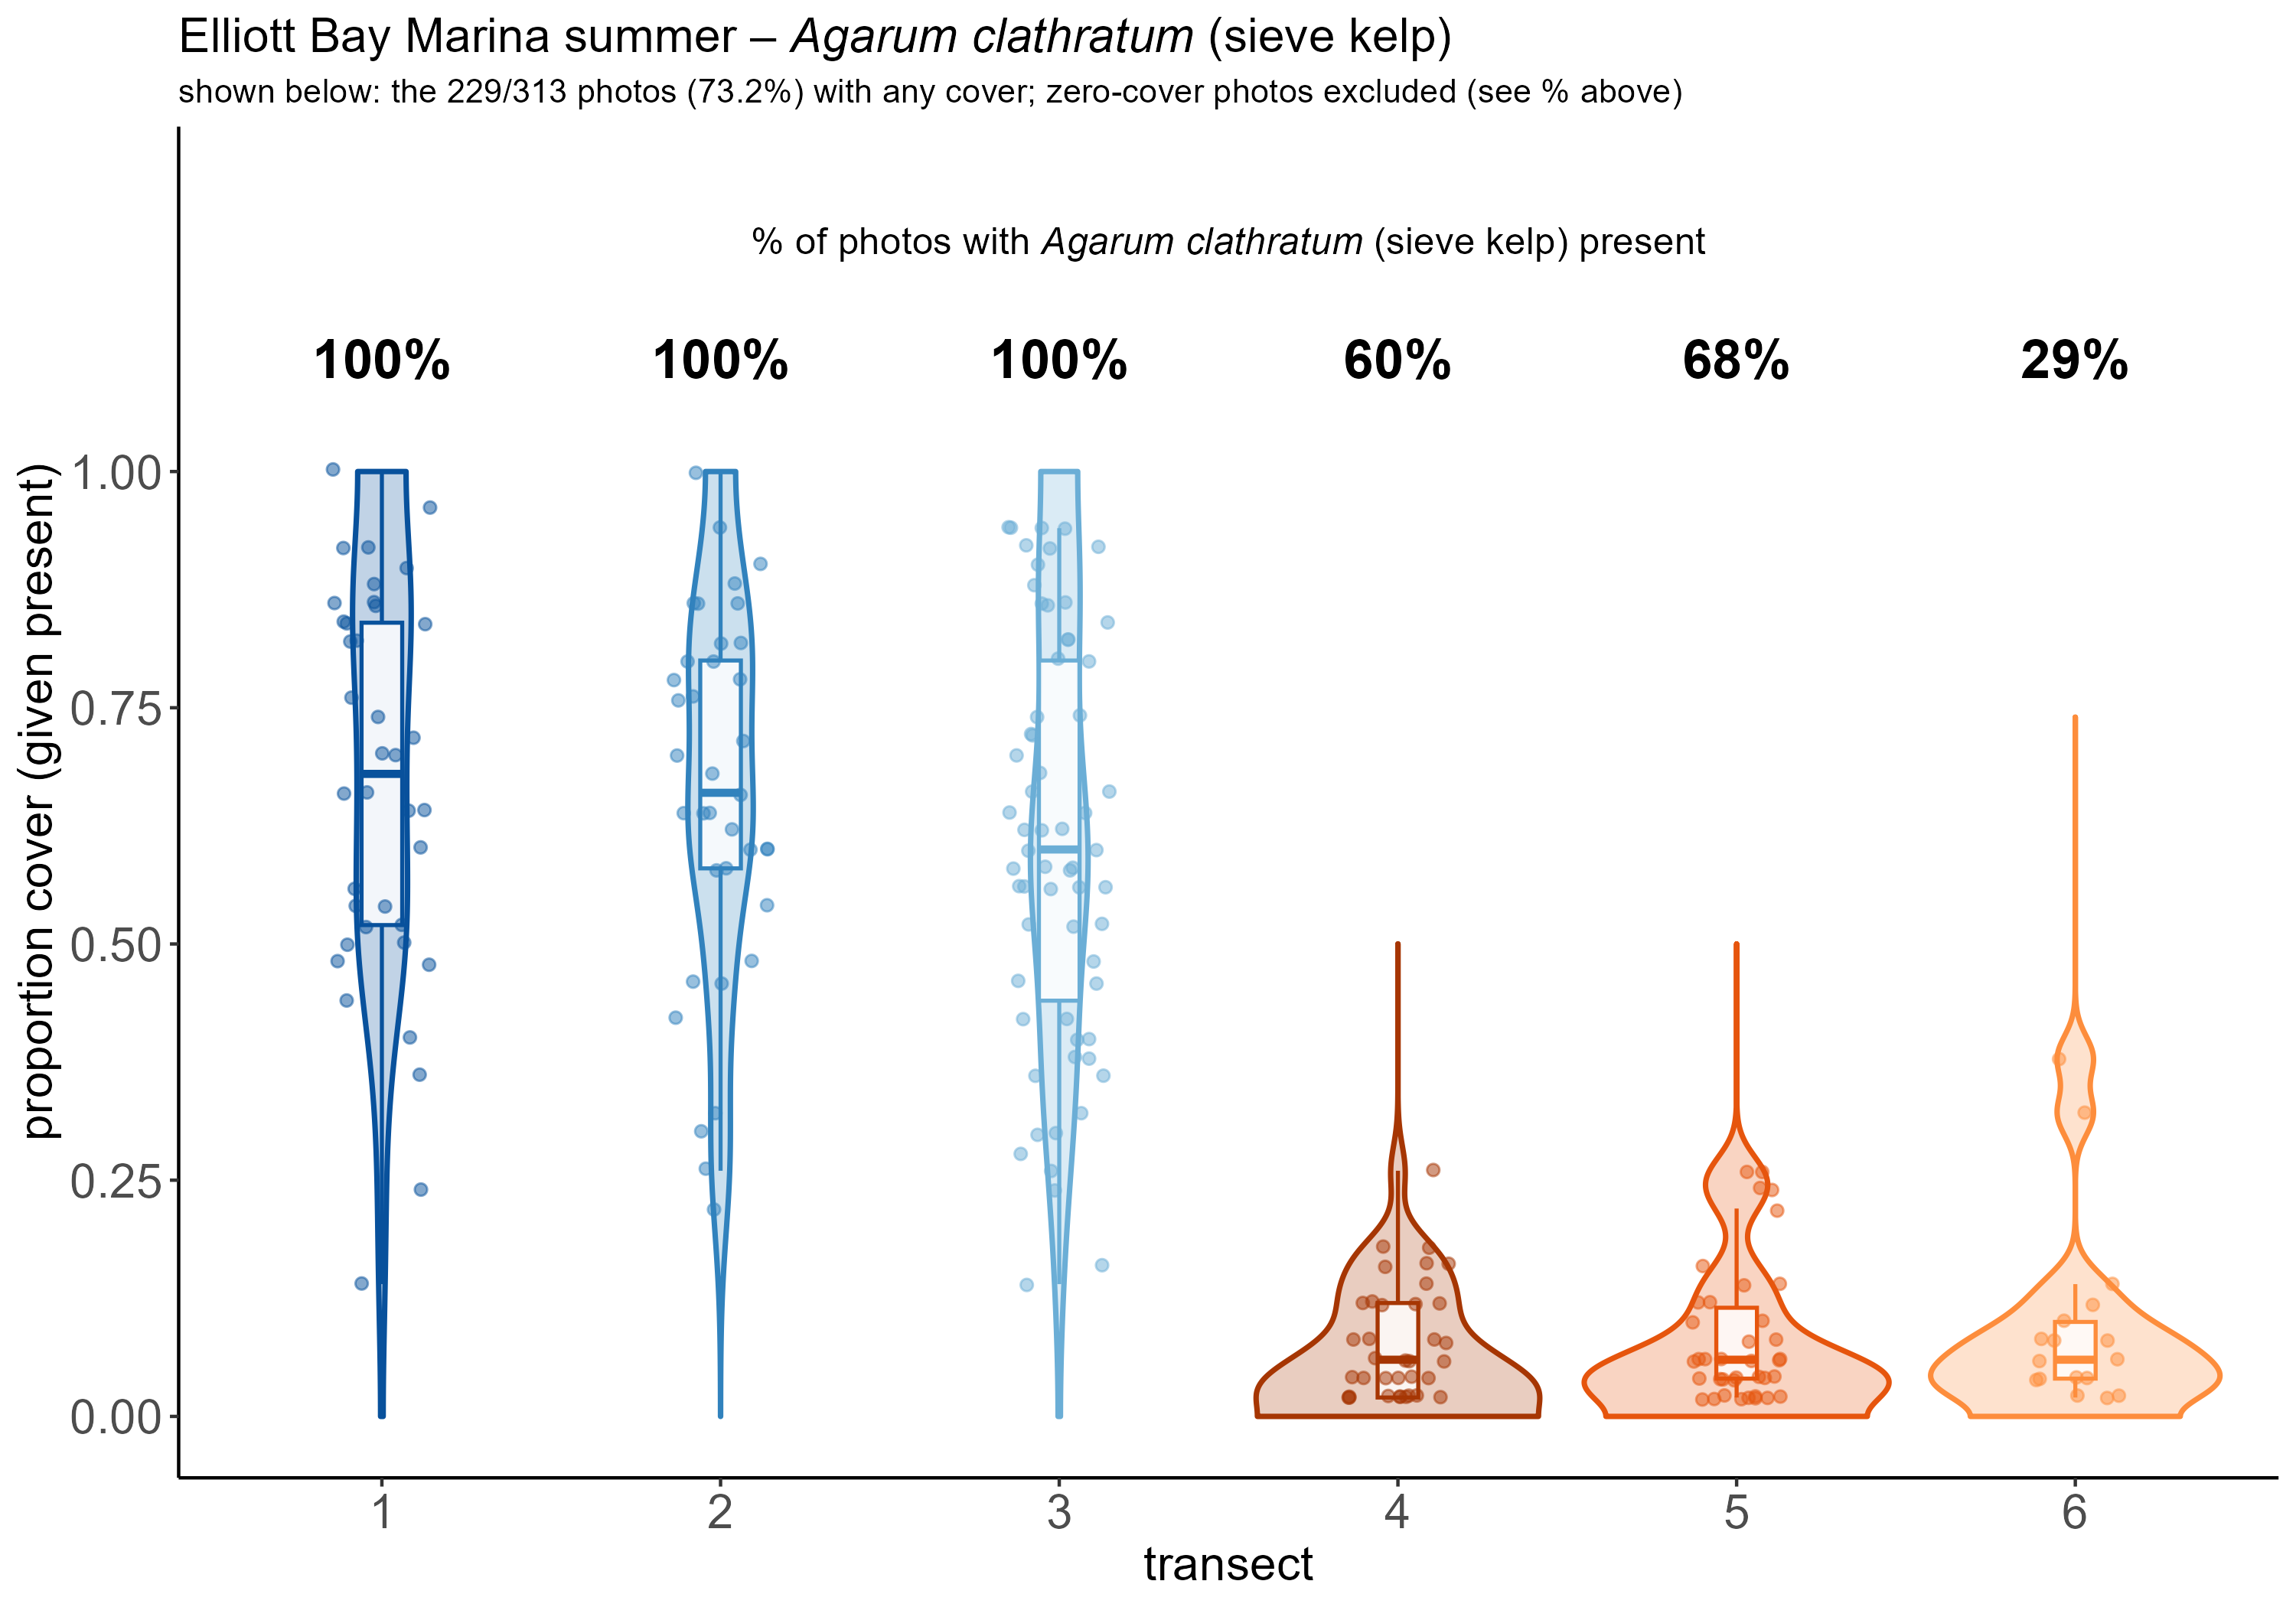
\includegraphics[width=0.98\textwidth]{violin.png}
\caption{
Photo-level distribution of \textit{Agarum clathratum} (sieve kelp)
percent-cover at Elliott Bay Marina, summer 2024, across all six transects.
Violin and box-and-whisker overlays summarize the distribution of per-photo
cover among photos where sieve kelp was present (individual points); the
percentage above each panel is the share of that transect's photos with any
sieve kelp present.
Transects 1--3 (deep) show sieve kelp present in 100\% of photos with a
broad, high-cover distribution (median 60--68\%), while transects 4--6
(shallow --- a 5\,m difference in depth from transects 1--3) show
substantially lower prevalence (29--68\% of photos) and a distribution
concentrated near zero cover.
}
\label{fig:violin}
\end{figure}
\vfil
}


\clearpage

\vbox to \textheight{
\vfil
\begin{figure}[H]
\centering
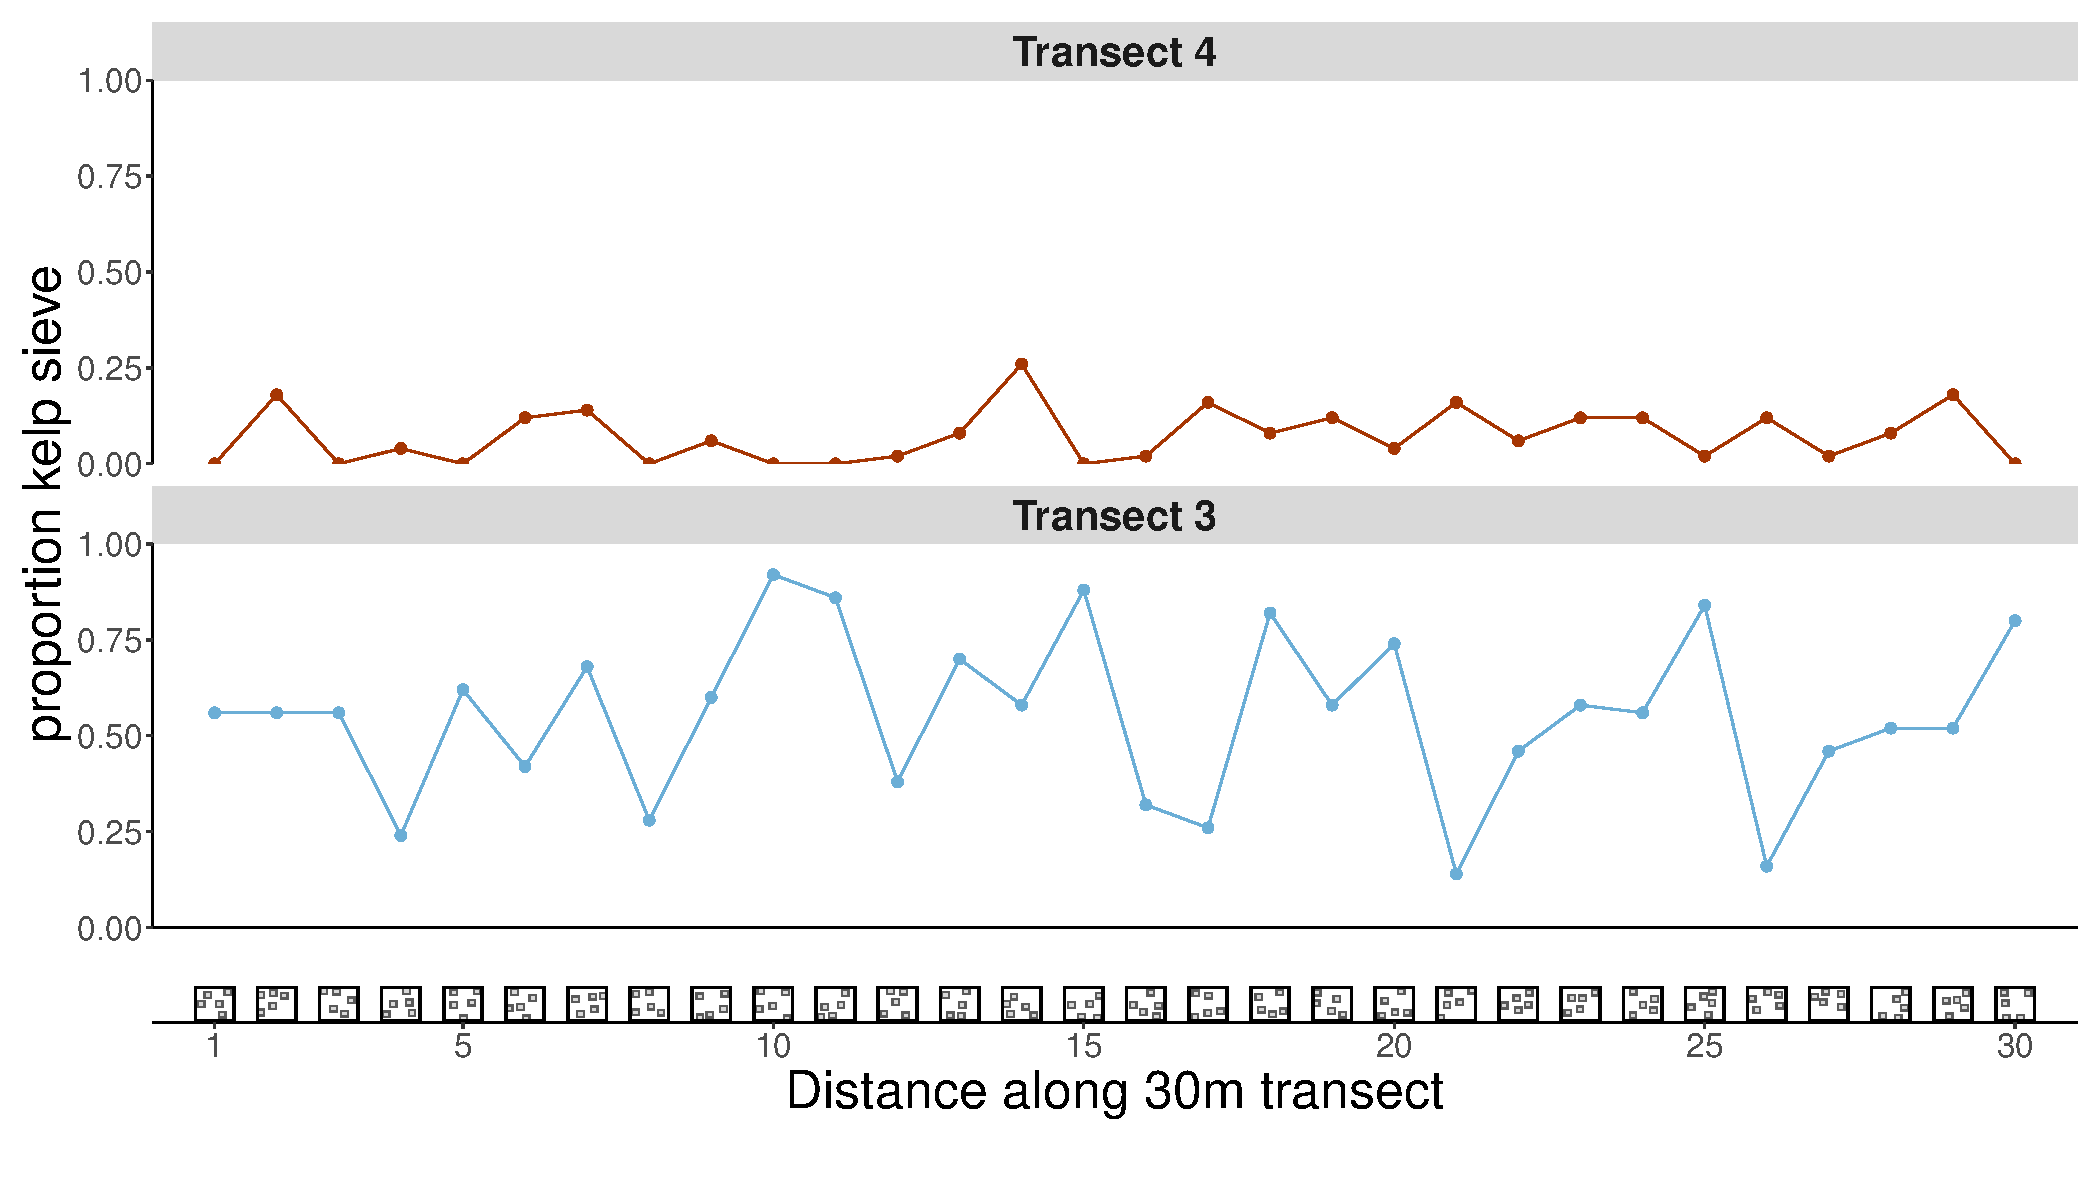
\includegraphics[width=0.98\textwidth]{proportion_across_space.pdf}
\caption{
ROV-recorded proportion of \textit{Agarum clathratum} (sieve kelp) at each
photograph along the 30\,m transect tape, Elliott Bay Marina summer 2024, for
transect 4 (shallow, top) and transect 3 (deep, bottom; the same two
transects summarized in \figref{fig:violin}).
Icons along the x-axis schematically represent individual ROV photographs (not 
to scale).
Transect 4 shows uniformly low cover throughout, with no obvious spatial
structure; transect 3 shows cover present at every point sampled, fluctuating
between roughly 15\% and 90\% in a patchy, quasi-repeating pattern with peaks
recurring roughly every 4--6\,m along the transect.
}
\label{fig:proportion_across_space}
\end{figure}
\vfil
}


\clearpage

\vbox to \textheight{
\vfil
\begin{figure}[H]
\centering
\begin{subfigure}[t]{0.48\textwidth}
\centering
\textbf{(a)}\par
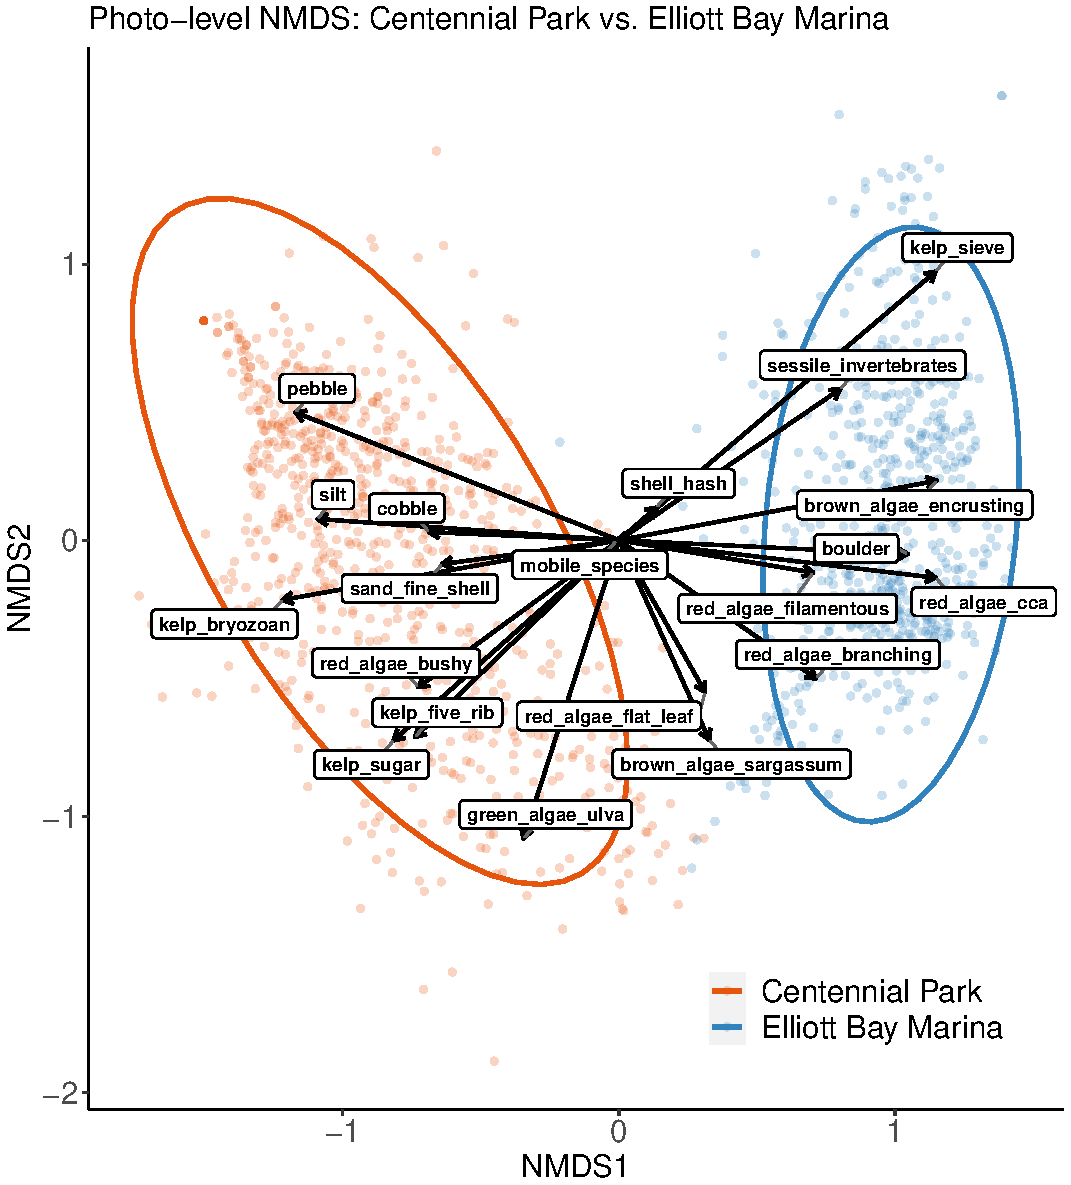
\includegraphics[width=\linewidth]{NMDS_1.pdf}
\end{subfigure}
\hspace{0.01\textwidth}
\begin{subfigure}[t]{0.48\textwidth}
\centering
\textbf{(b)}\par
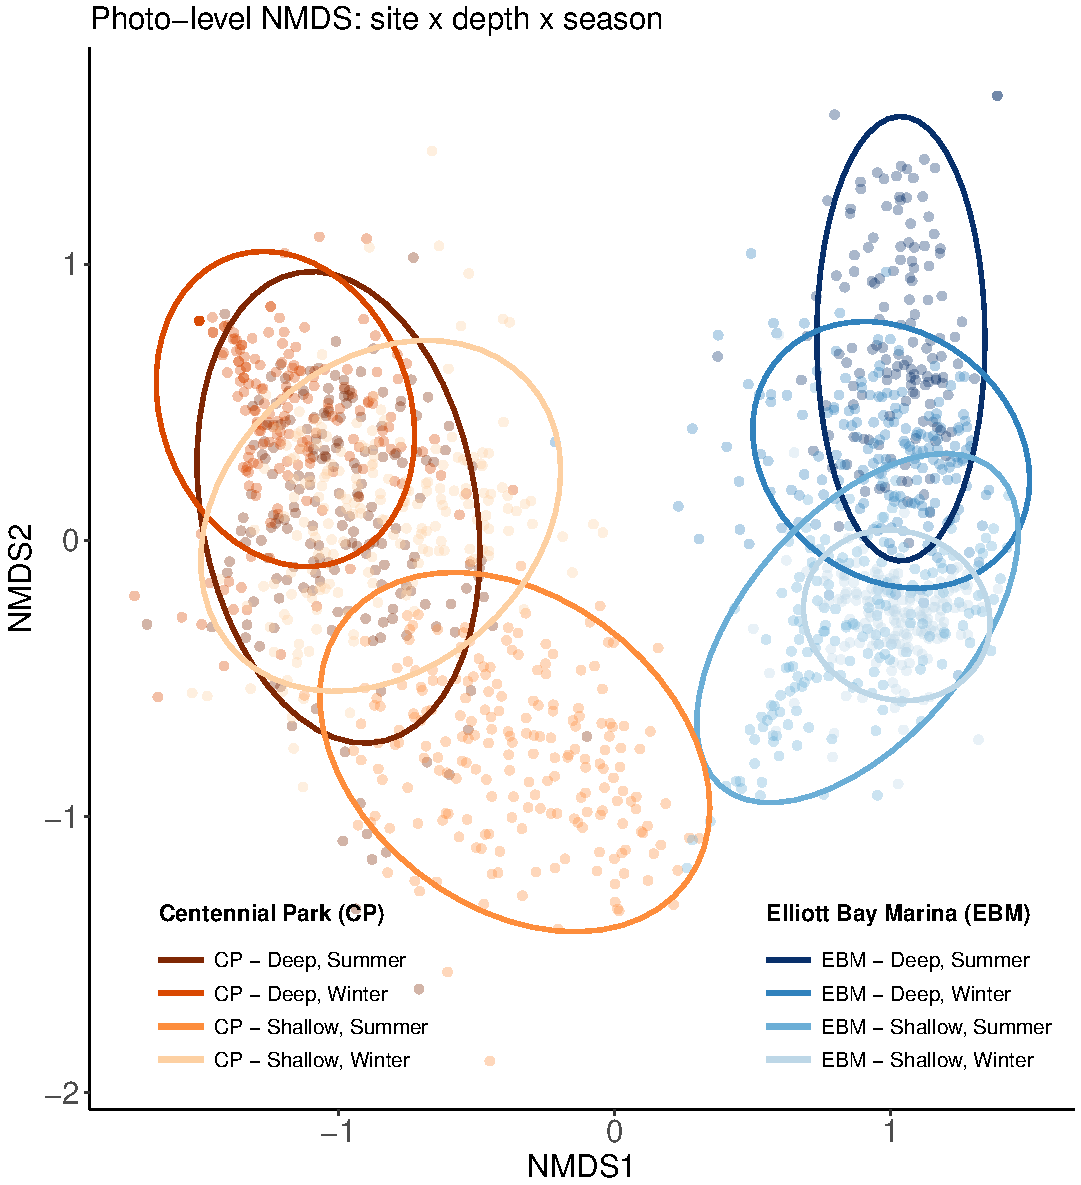
\includegraphics[width=\linewidth]{NMDS_2.pdf}
\end{subfigure}
\caption{
Non-metric multidimensional scaling (NMDS) ordination of ROV percent-cover
data at the photograph level (Bray-Curtis dissimilarity, $k=2$, stress
$=0.134$, $n=1{,}436$ photos across 30 percent-cover categories), with 95\%
confidence ellipses.
\textbf{(a)} Ordination colored by site, with category-correlation vectors
overlaid: Centennial Park's community is associated with soft-substrate
categories (pebble, silt, cobble, sand) and sugar kelp, while Elliott Bay
Marina's is associated with hard-substrate categories (boulder, crustose
coralline algae) and sieve kelp, consistent with the two sites' contrasting
substrate types.
\textbf{(b)} The same ordination colored by site $\times$ depth $\times$
season (8 groups).
Between-site separation dominates the ordination, but within each site, deep
and shallow transects also separate along NMDS2, most clearly at Elliott Bay
Marina, where the two depth strata's ellipses show only modest overlap;
season contributes comparatively little additional separation within a site
and depth.
}
\label{fig:NMDS}
\end{figure}
\vfil
}

\clearpage

\vbox to \textheight{%
\vfil
\begin{figure}[H]
\centering
\begin{subfigure}[t]{0.495\textwidth}
\centering
\textbf{(a)}\par
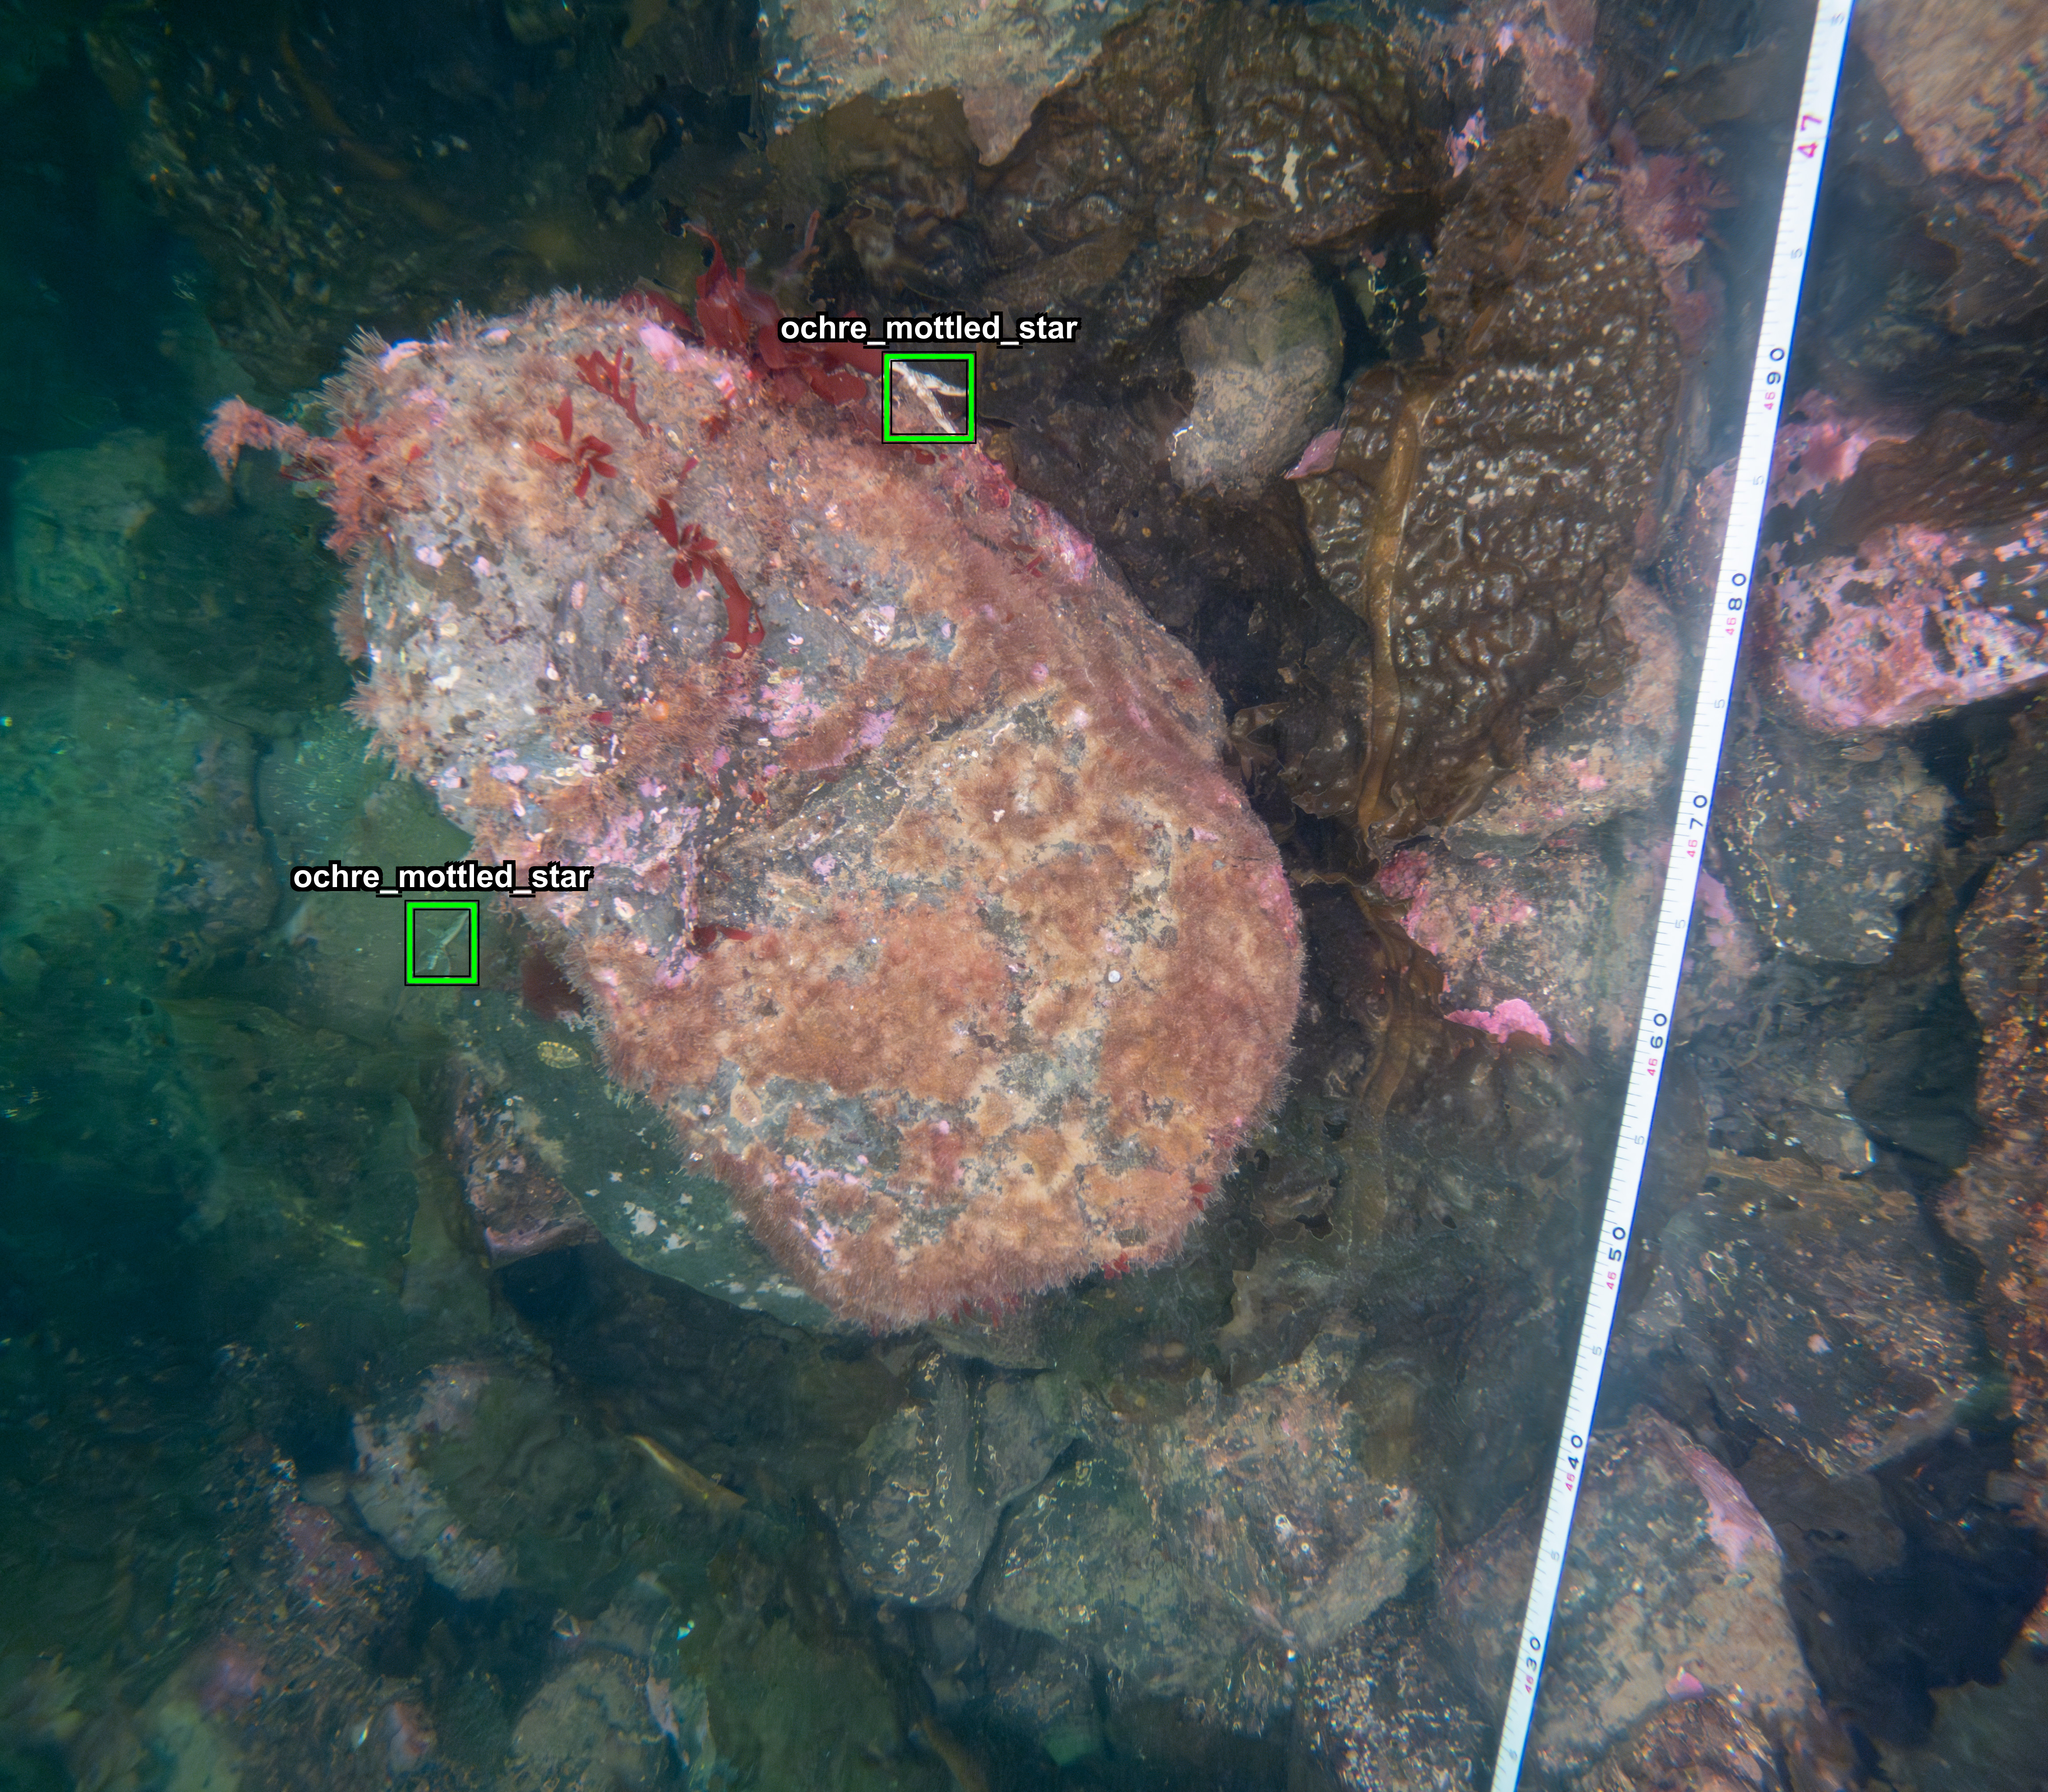
\includegraphics[width=\linewidth]{extra_width_1.jpg}
\end{subfigure}%
\hfill%
\begin{subfigure}[t]{0.495\textwidth}
\centering
\textbf{(b)}\par
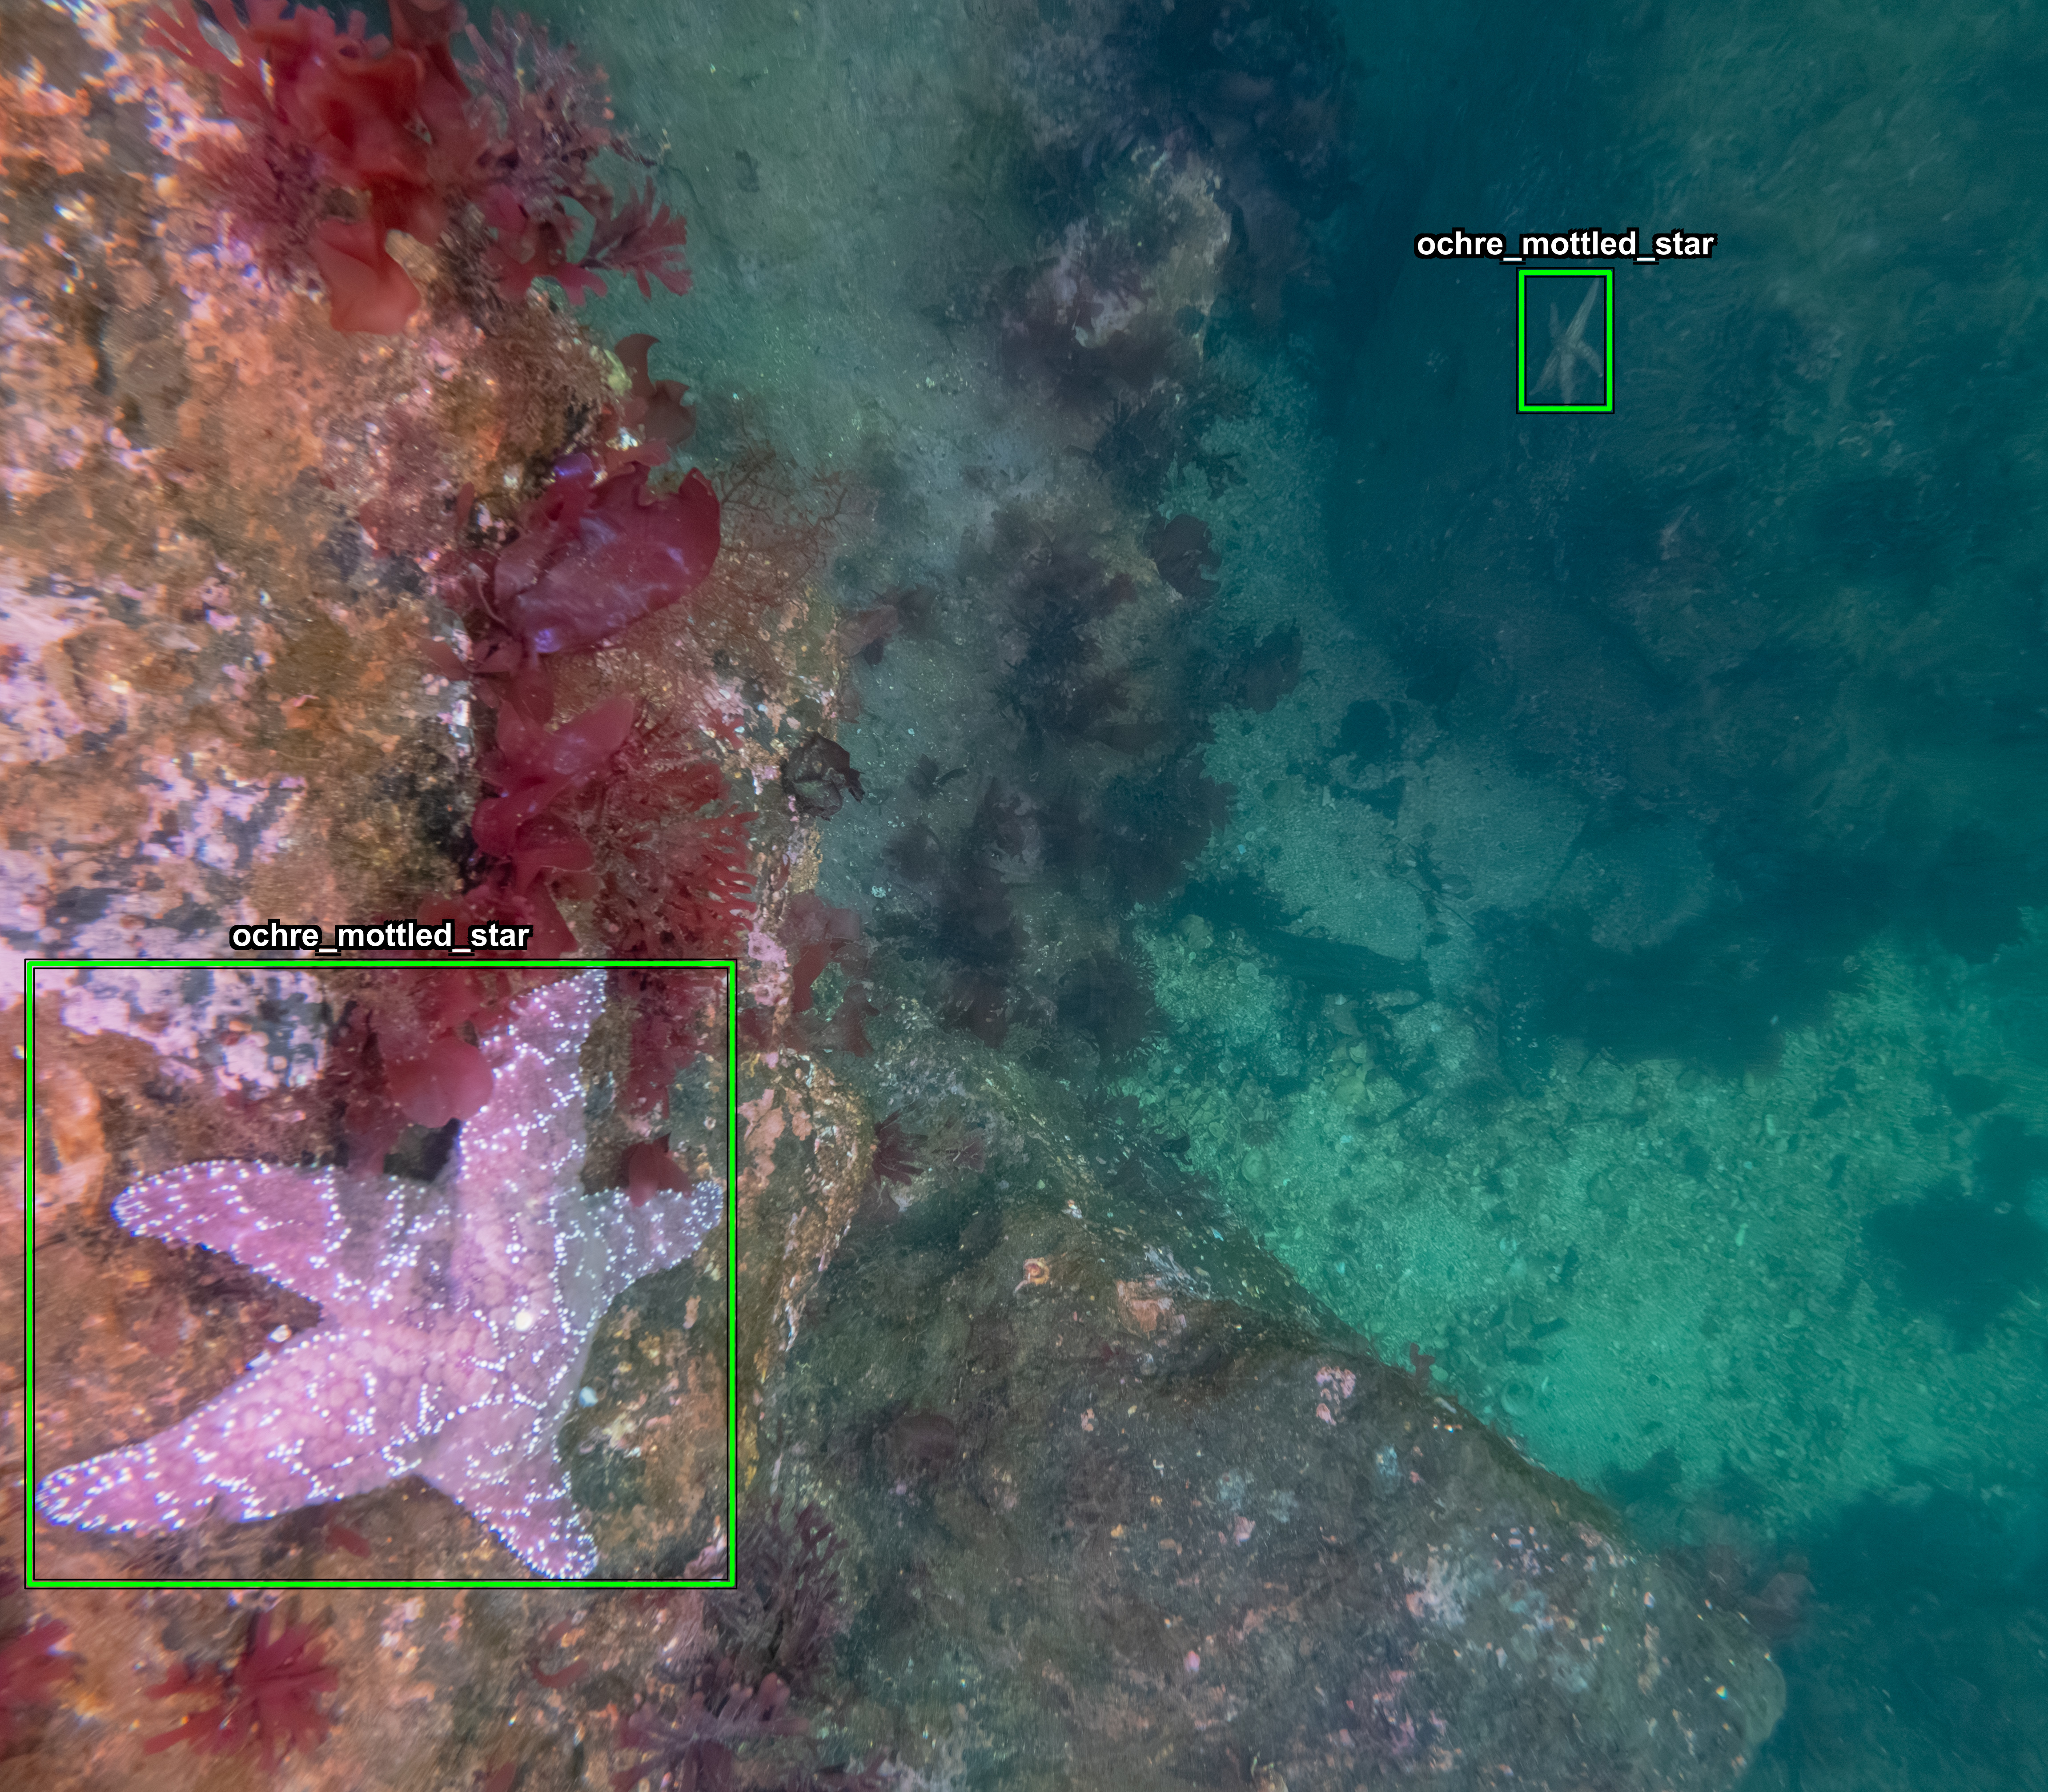
\includegraphics[width=\linewidth]{extra_width_2.jpg}
\end{subfigure}
\vspace{0.005\textheight}
\begin{subfigure}[t]{0.495\textwidth}
\centering
\textbf{(c)}\par
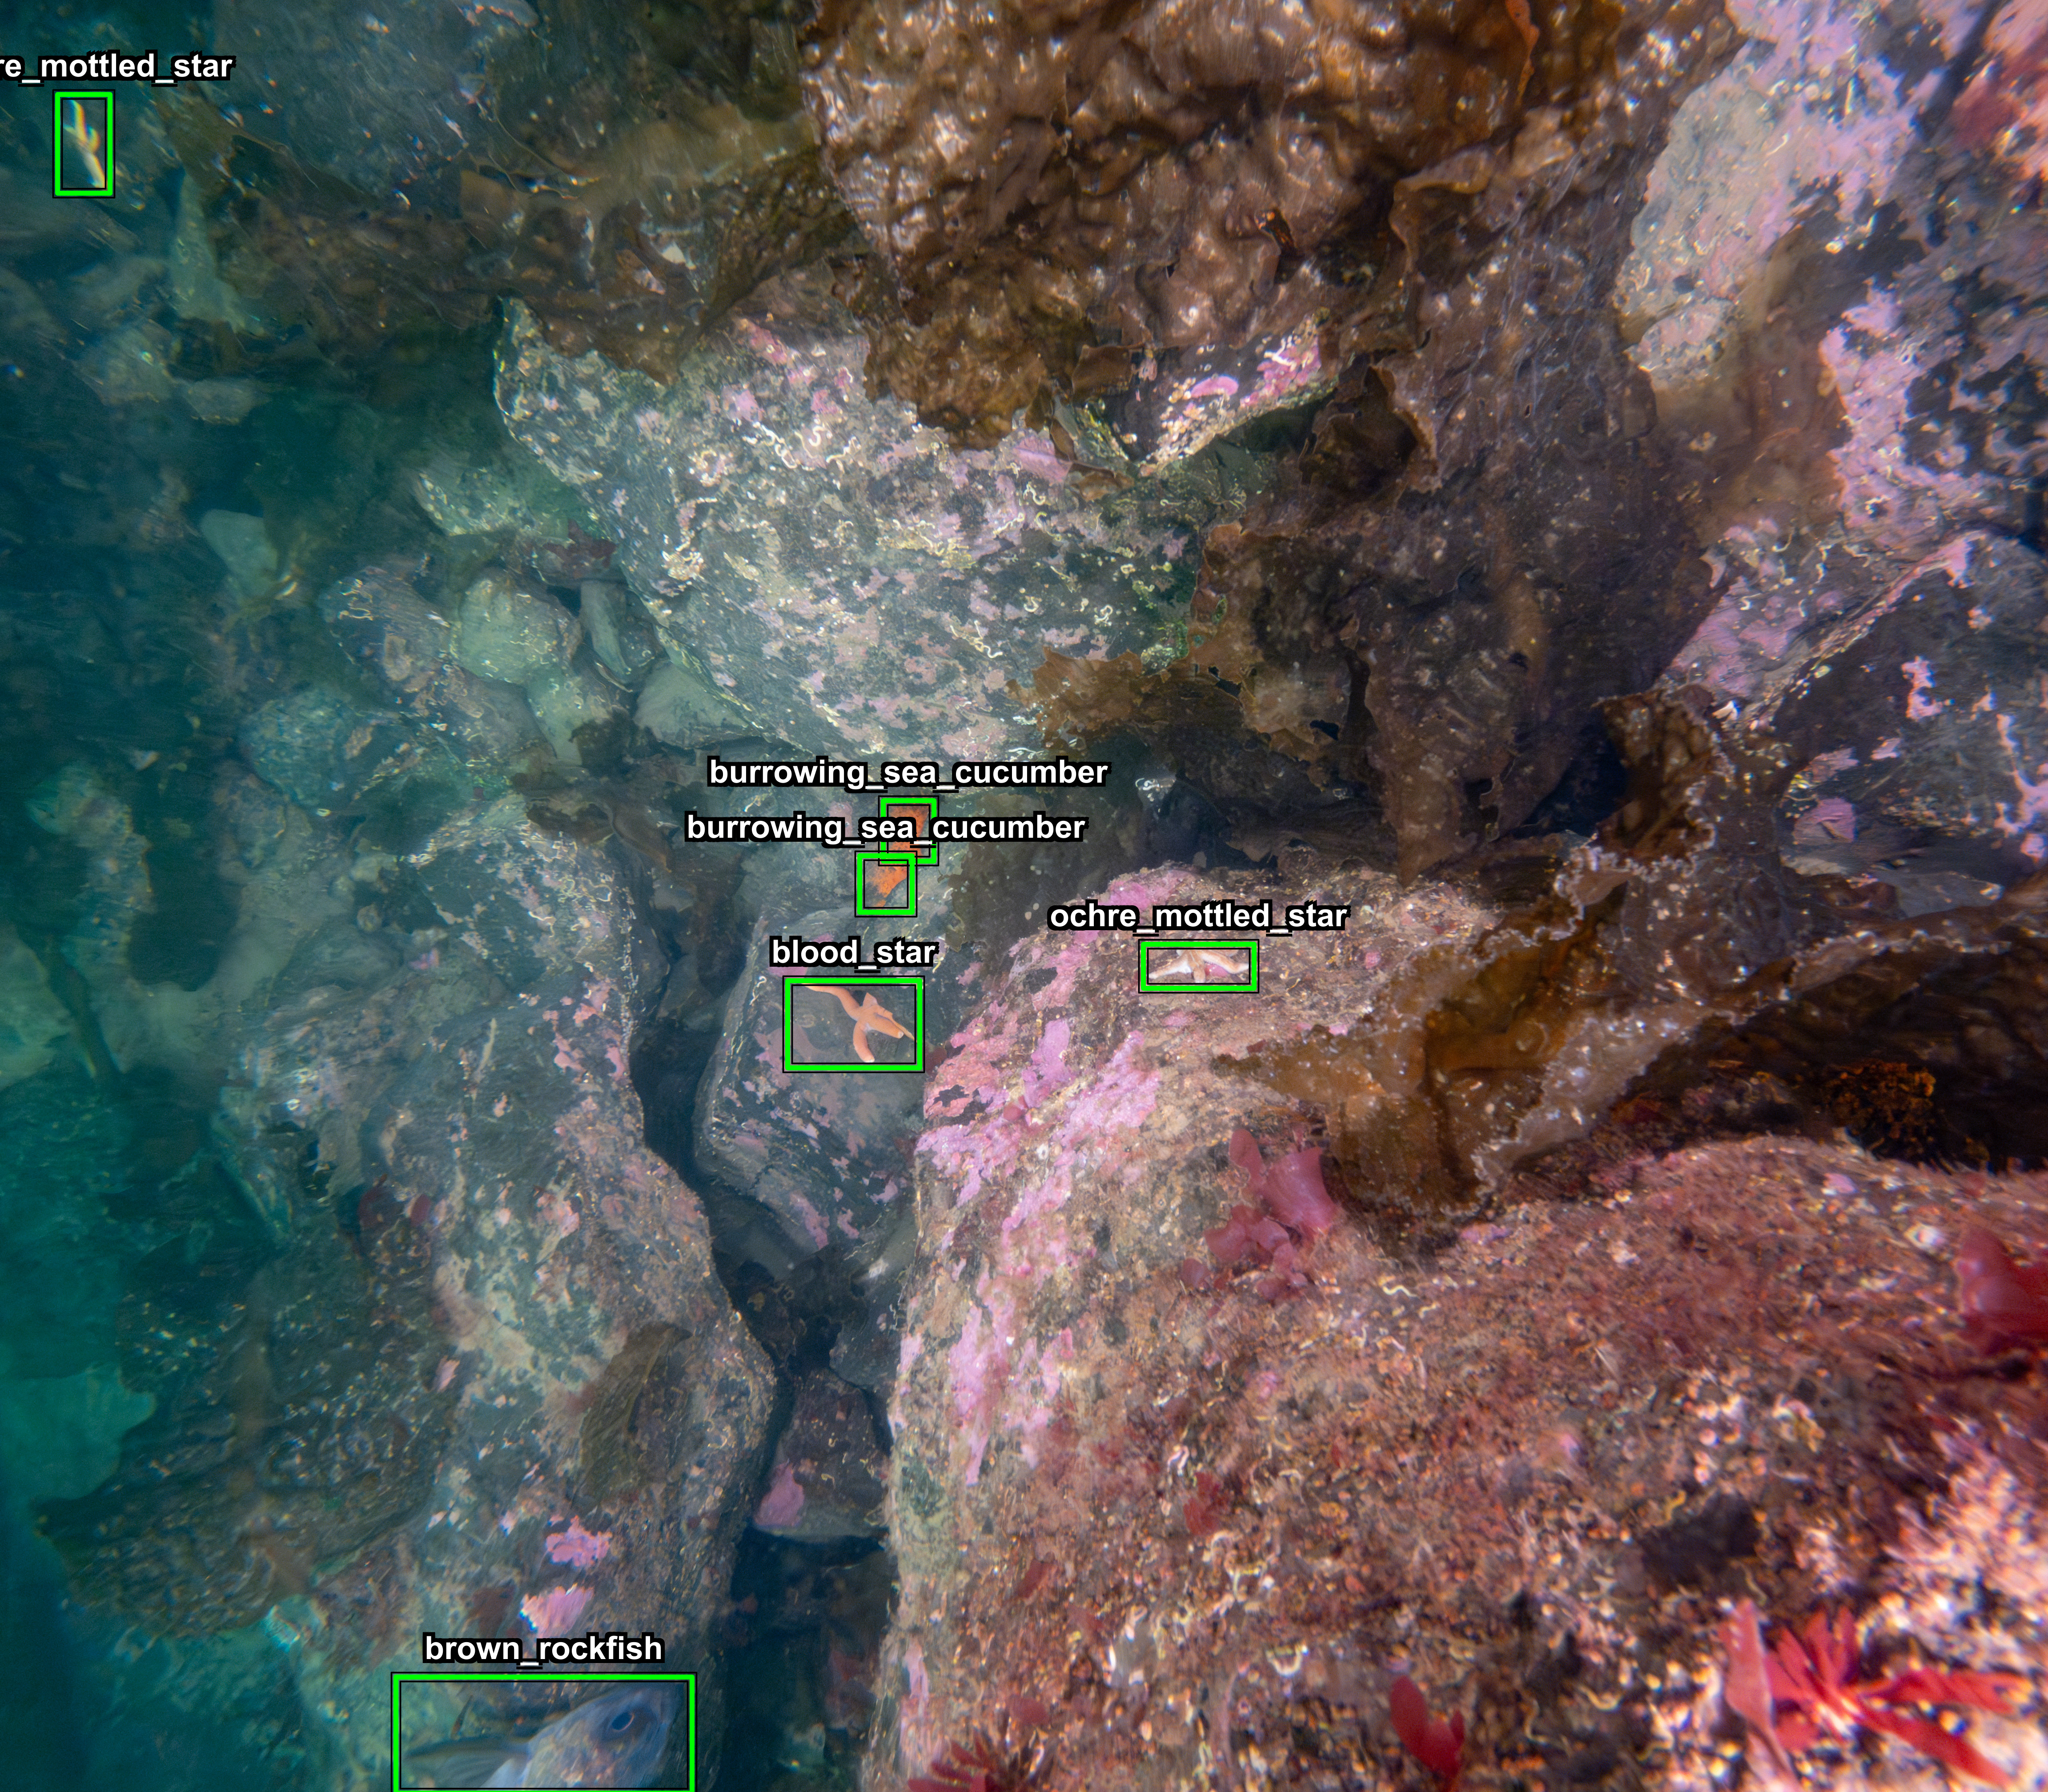
\includegraphics[width=\linewidth]{extra_width_3.jpg}
\end{subfigure}%
\hfill%
\begin{subfigure}[t]{0.495\textwidth}
\centering
\textbf{(d)}\par
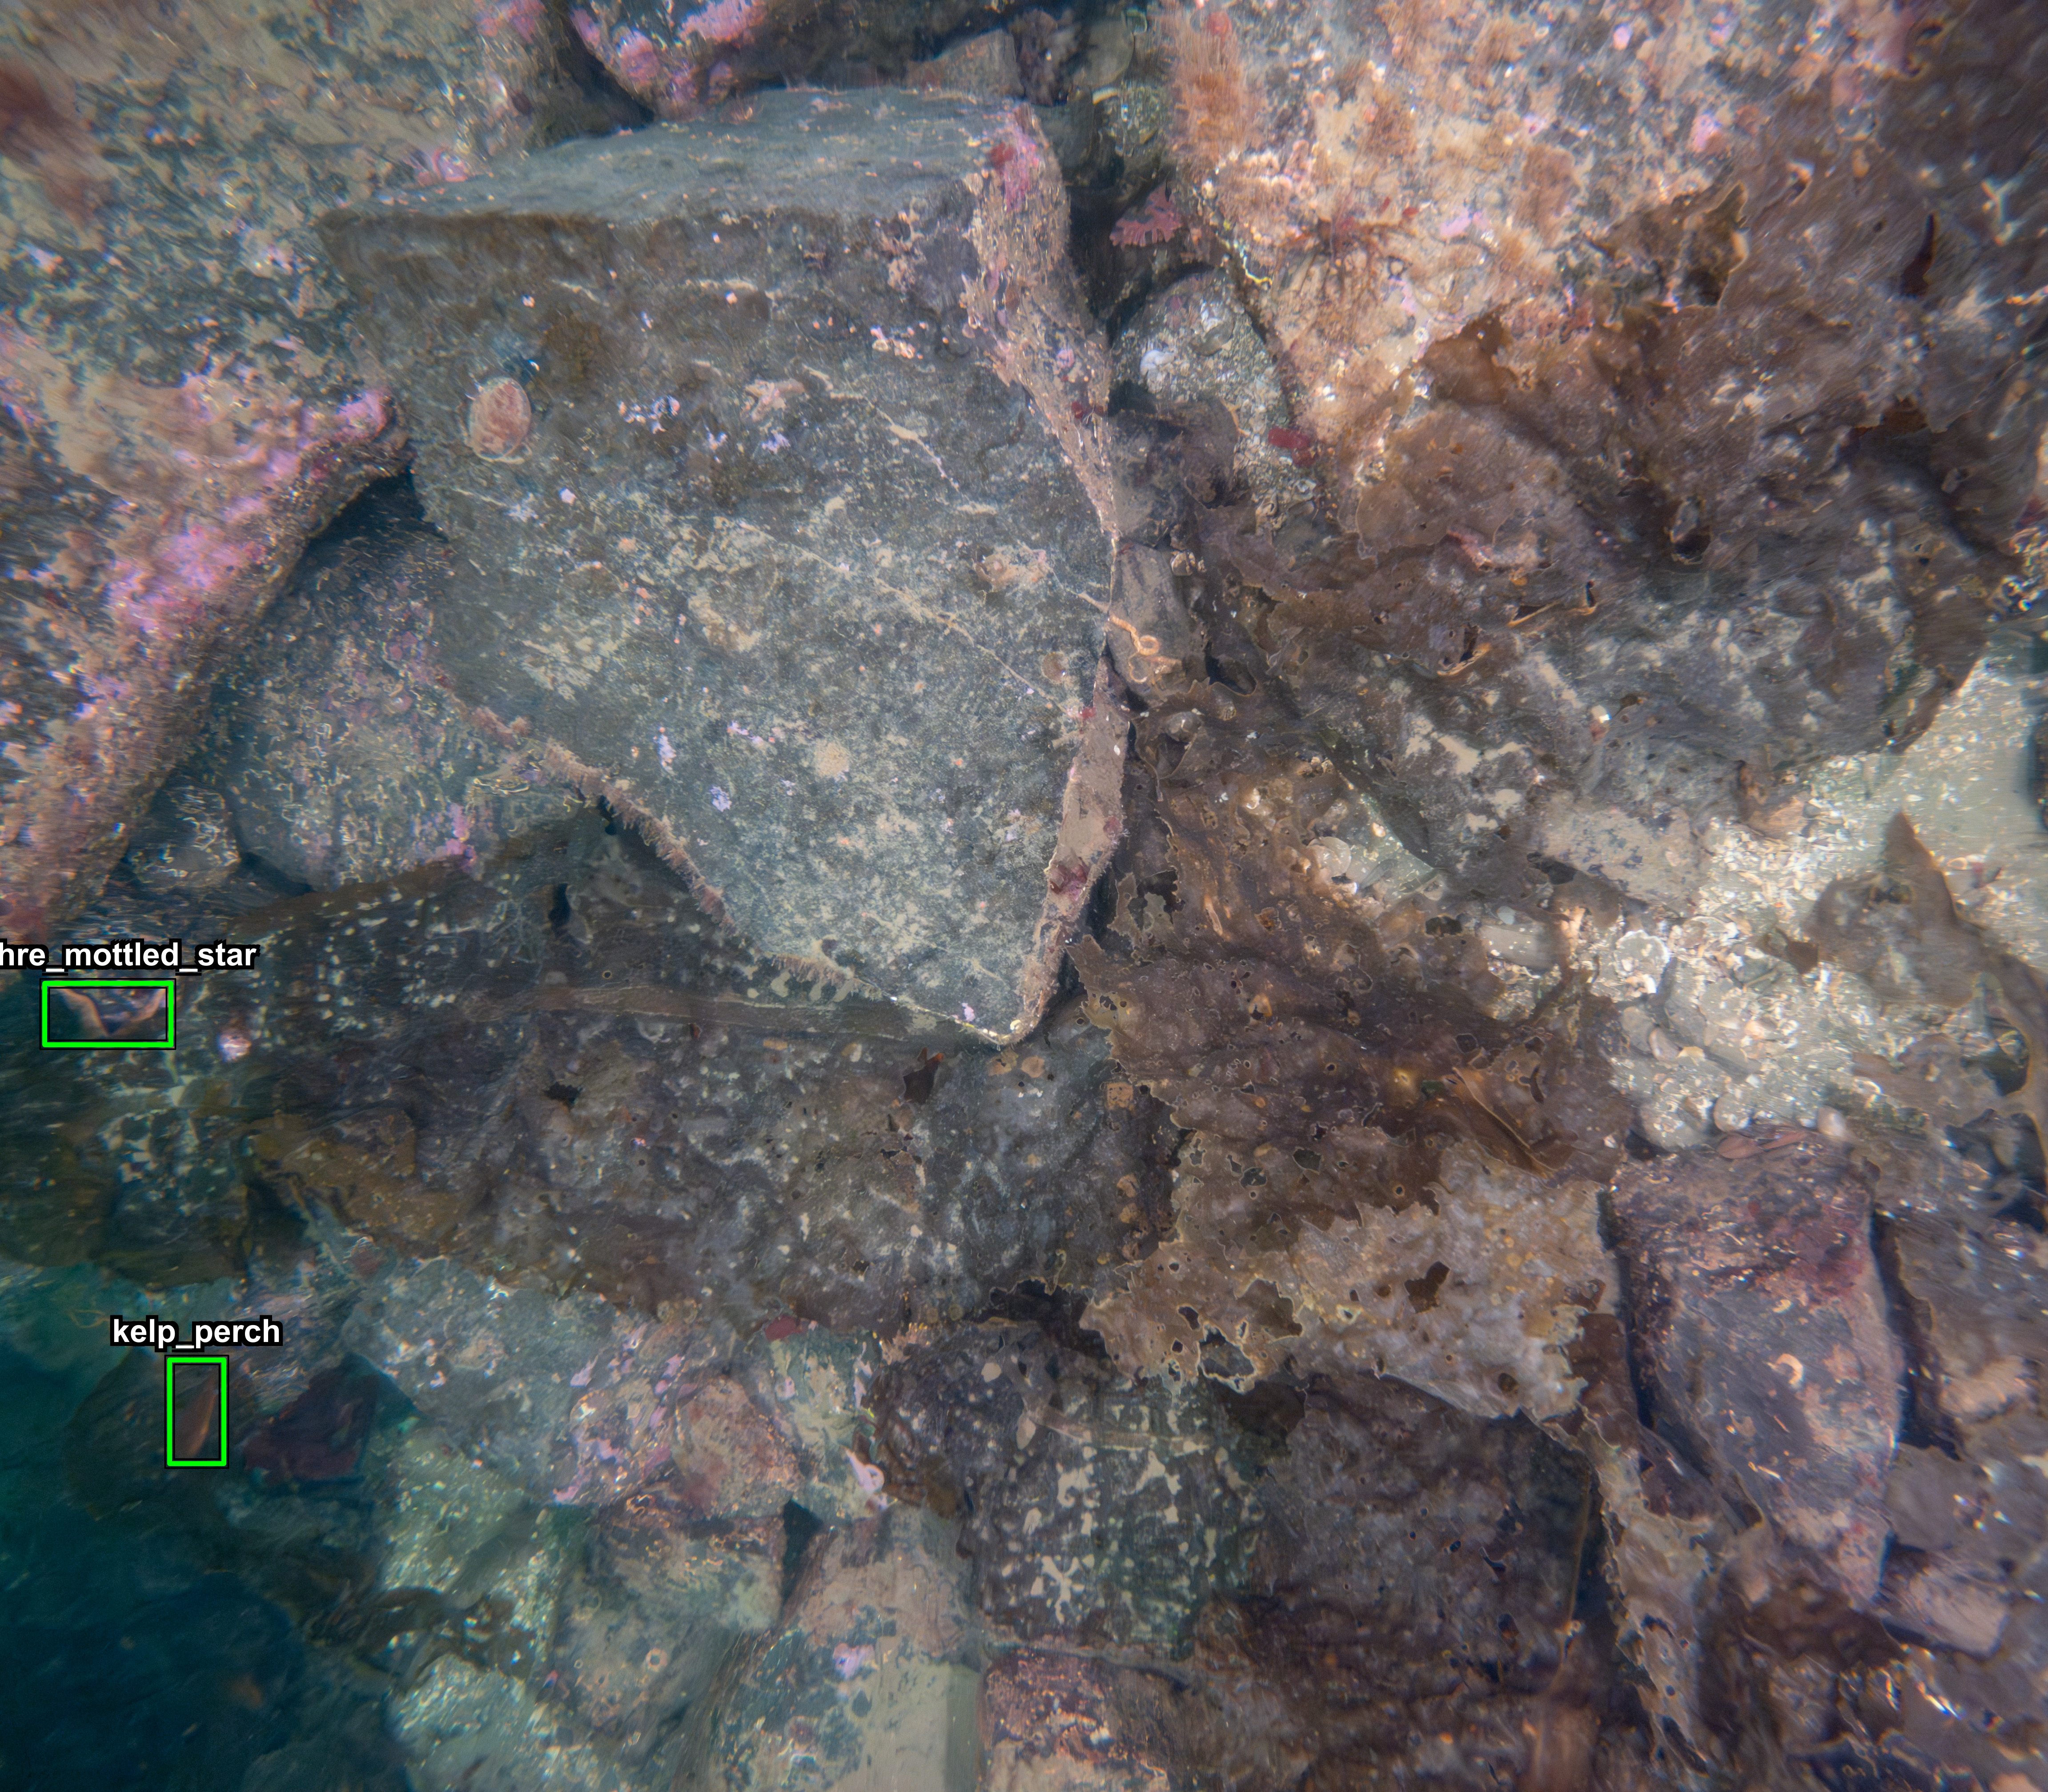
\includegraphics[width=\linewidth]{extra_width_4.jpg}
\end{subfigure}
\caption{
Four instances where the extra width of the GoPro's camera likely resulted in a 
non-linear increase in the amount of benthos photographed.
This non-linearity is especially present at the Elliott Bay Marina breakwater 
site, where the parallel ROV transects resulted in a depth contour being 
captured at the edge of most images.
The four images depicted here all include instances where species abundances 
were annotated that likely fell outside of the diver's $1~m$ swath transect, 
thus artificially increasing the ROV's total abundance counts. 
}
\label{fig:extra_width}
\end{figure}
\vfil
}

\clearpage

\vbox to \textheight{%
\vfil
\begin{figure}[H]
\centering
\begin{subfigure}[t]{0.495\textwidth}
\centering
\textbf{(a)}\par
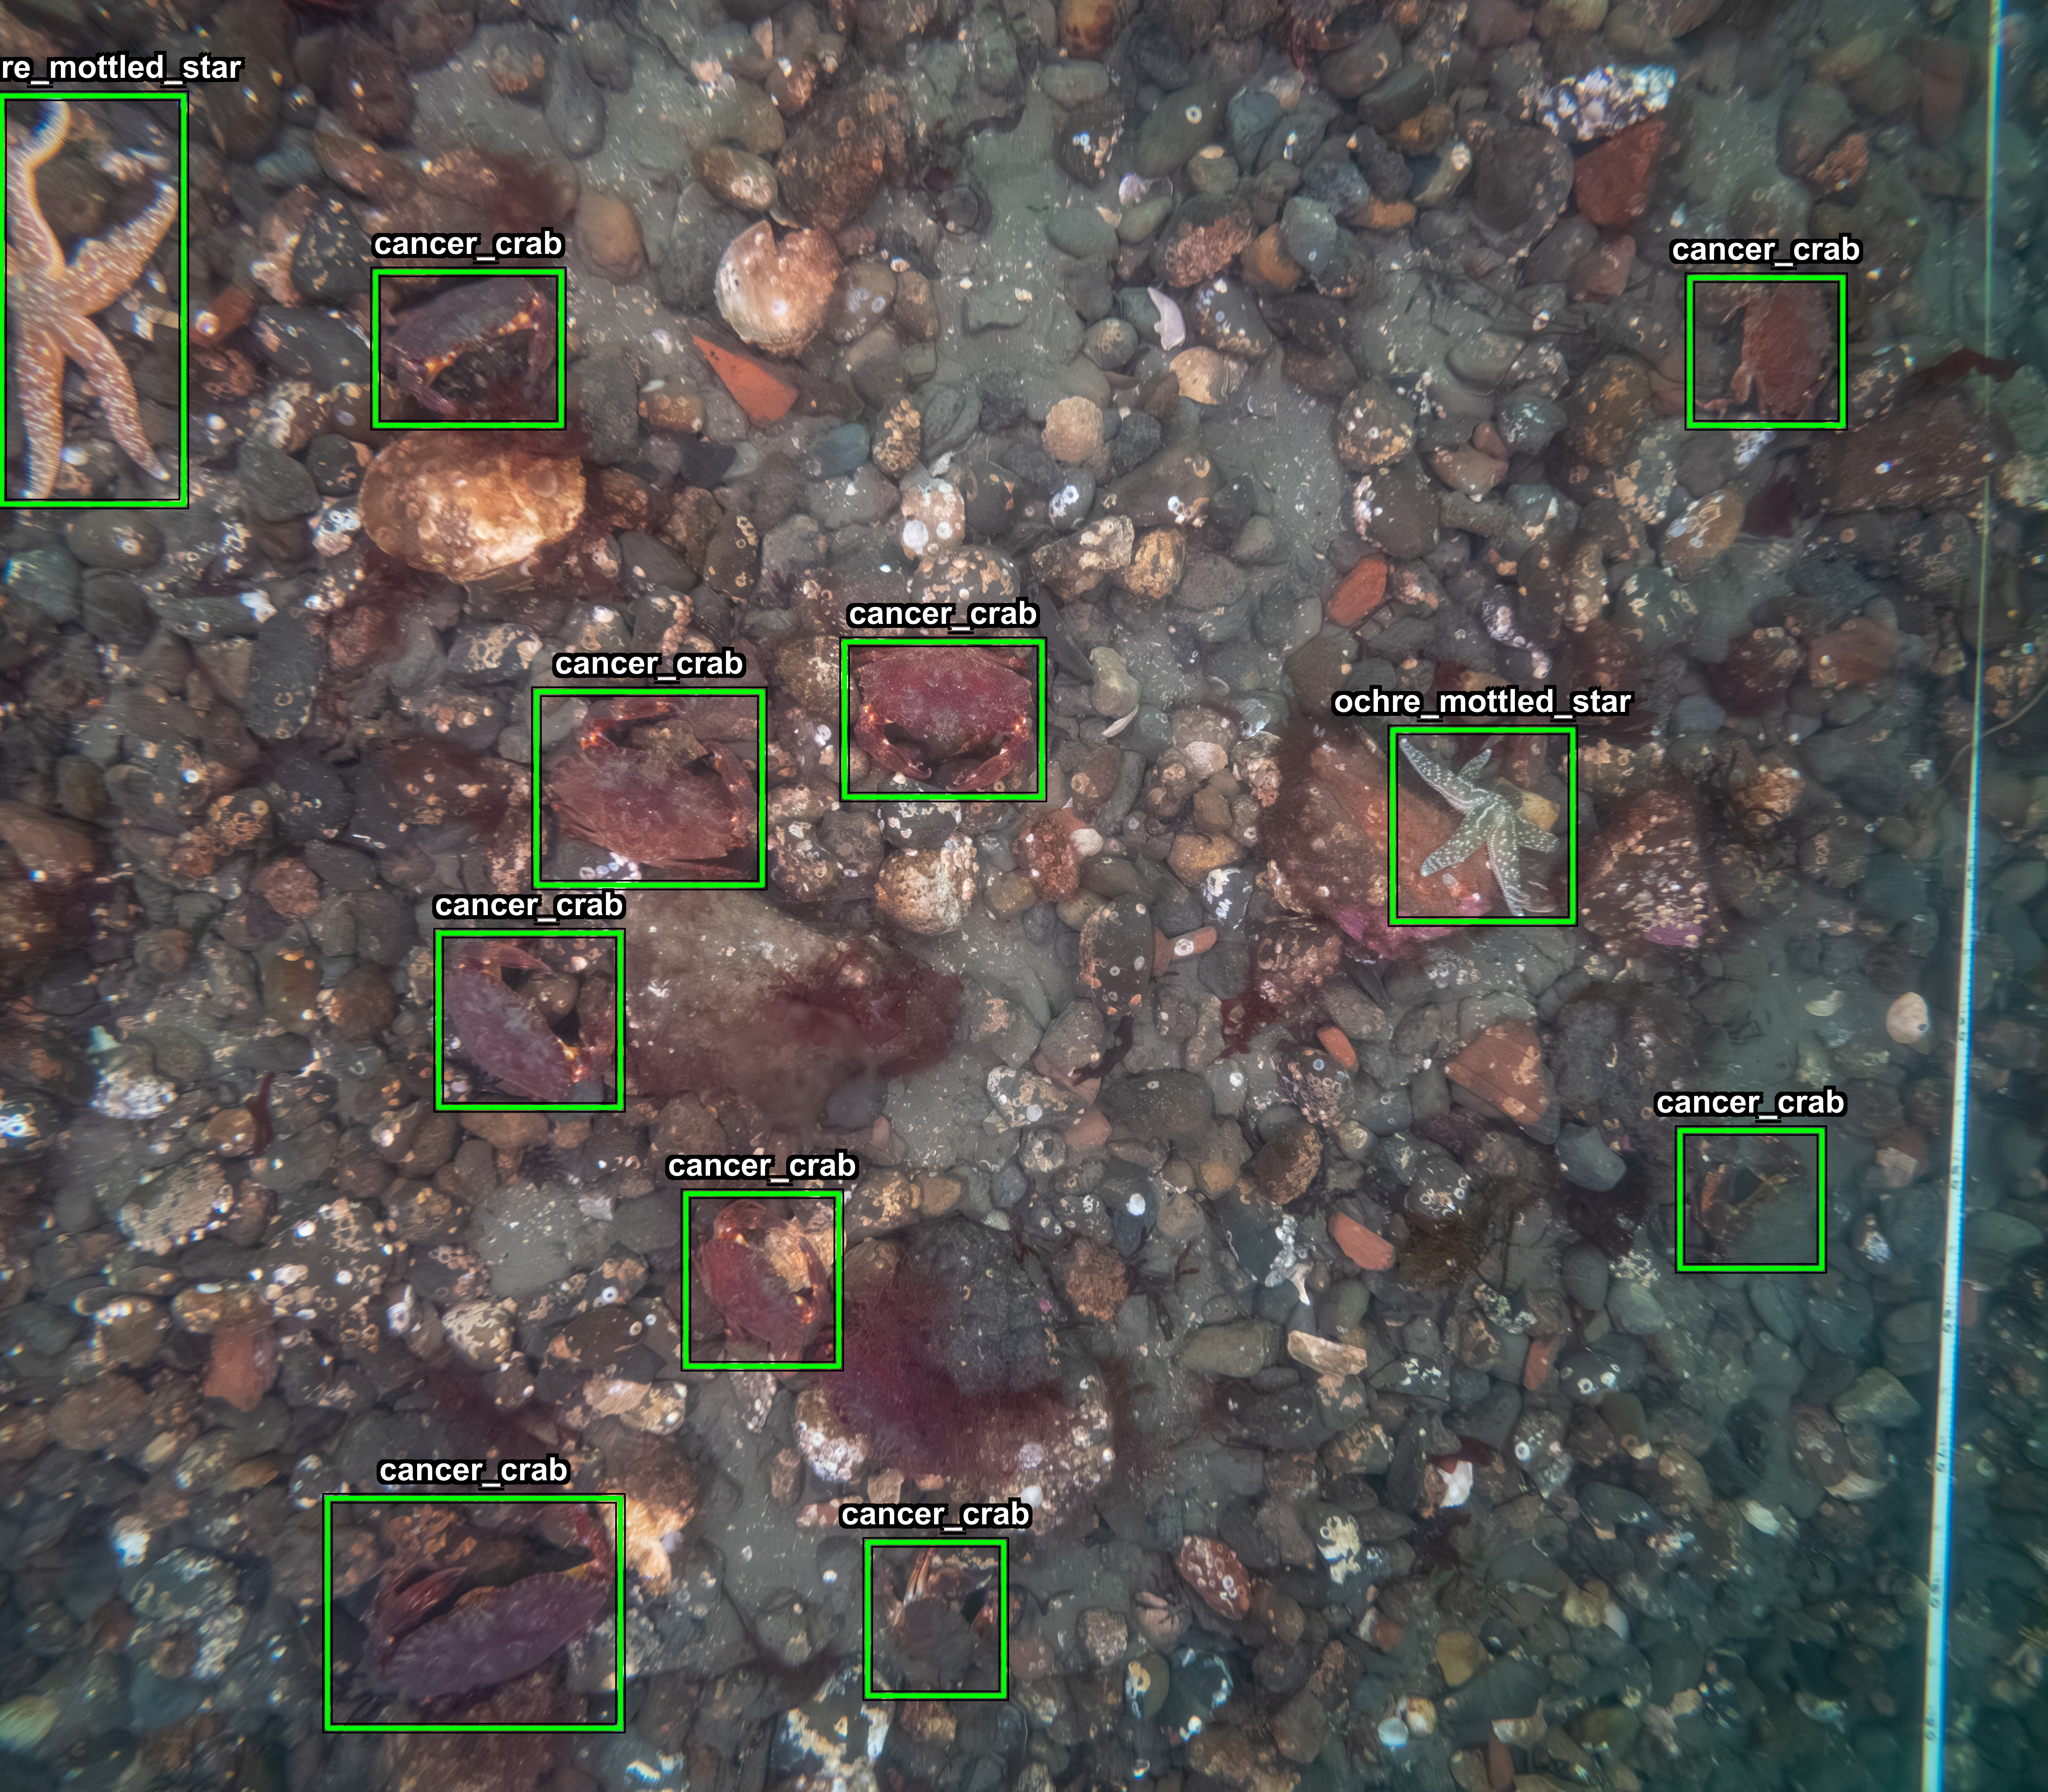
\includegraphics[width=\linewidth]{double_count_3.jpg}
\end{subfigure}%
\hfill%
\begin{subfigure}[t]{0.495\textwidth}
\centering
\textbf{(b)}\par
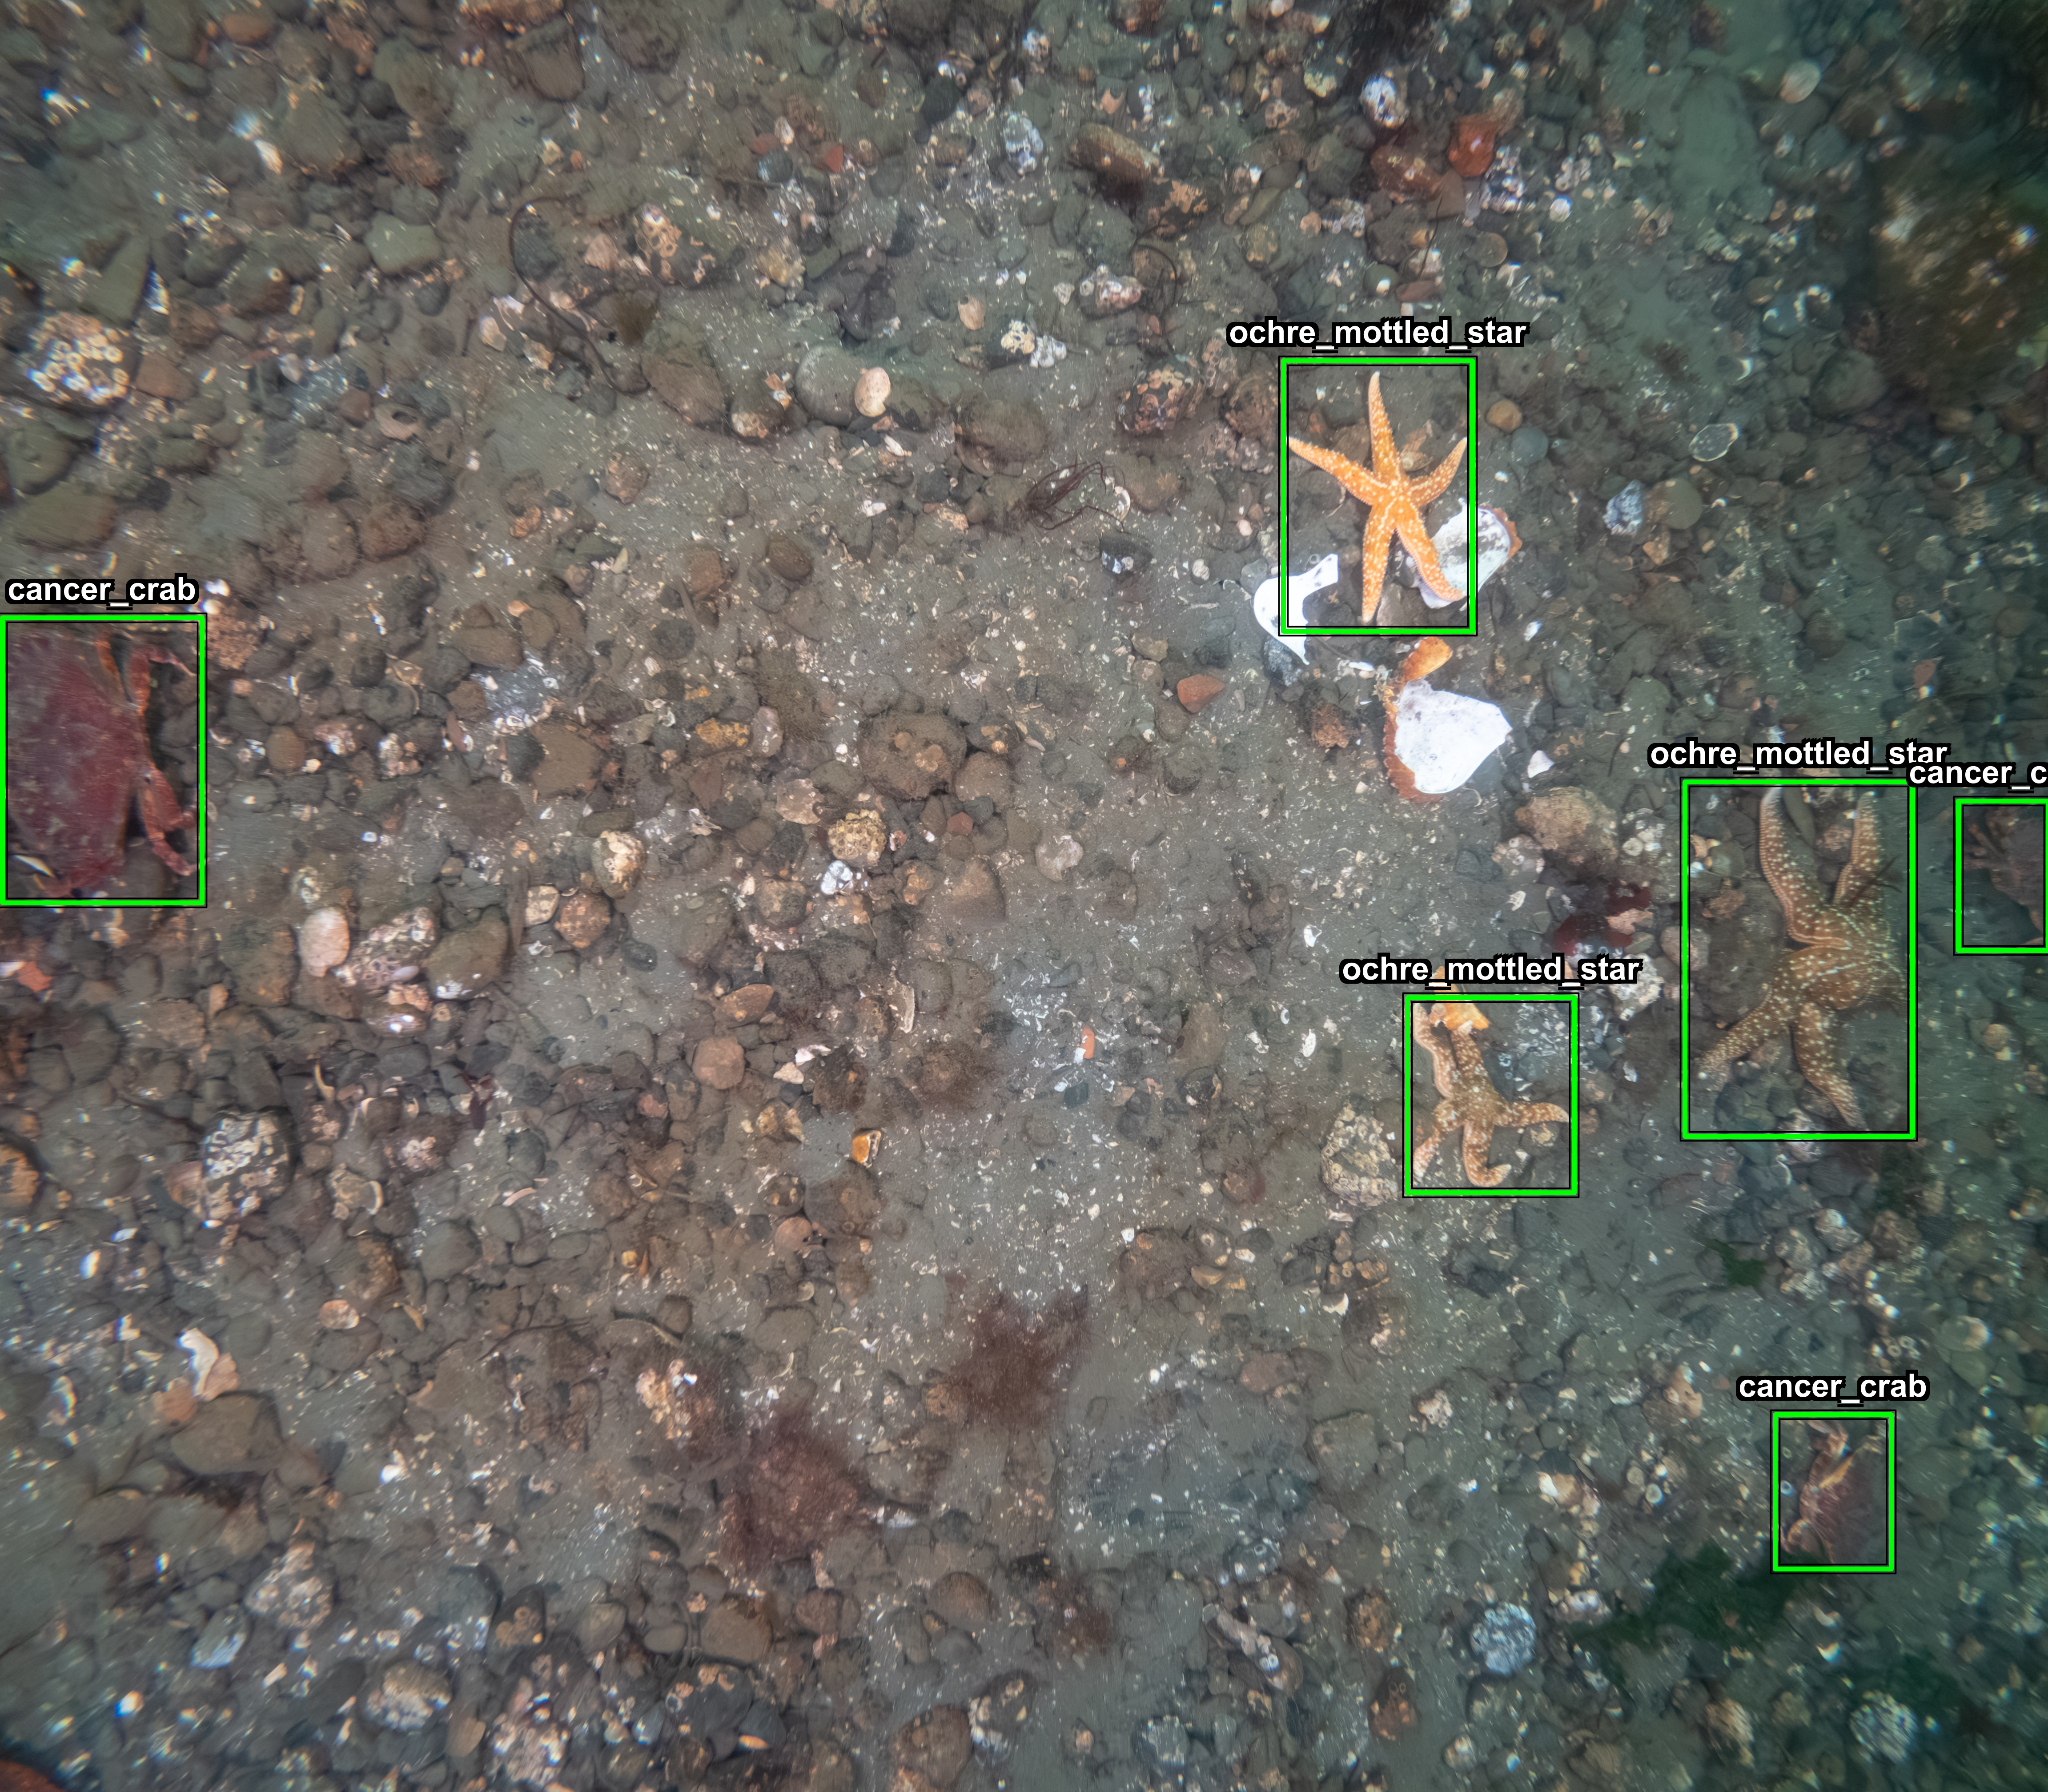
\includegraphics[width=\linewidth]{double_count_1.jpg}
\end{subfigure}
\vspace{0.005\textheight}
\begin{subfigure}[t]{0.495\textwidth}
\centering
\textbf{(c)}\par
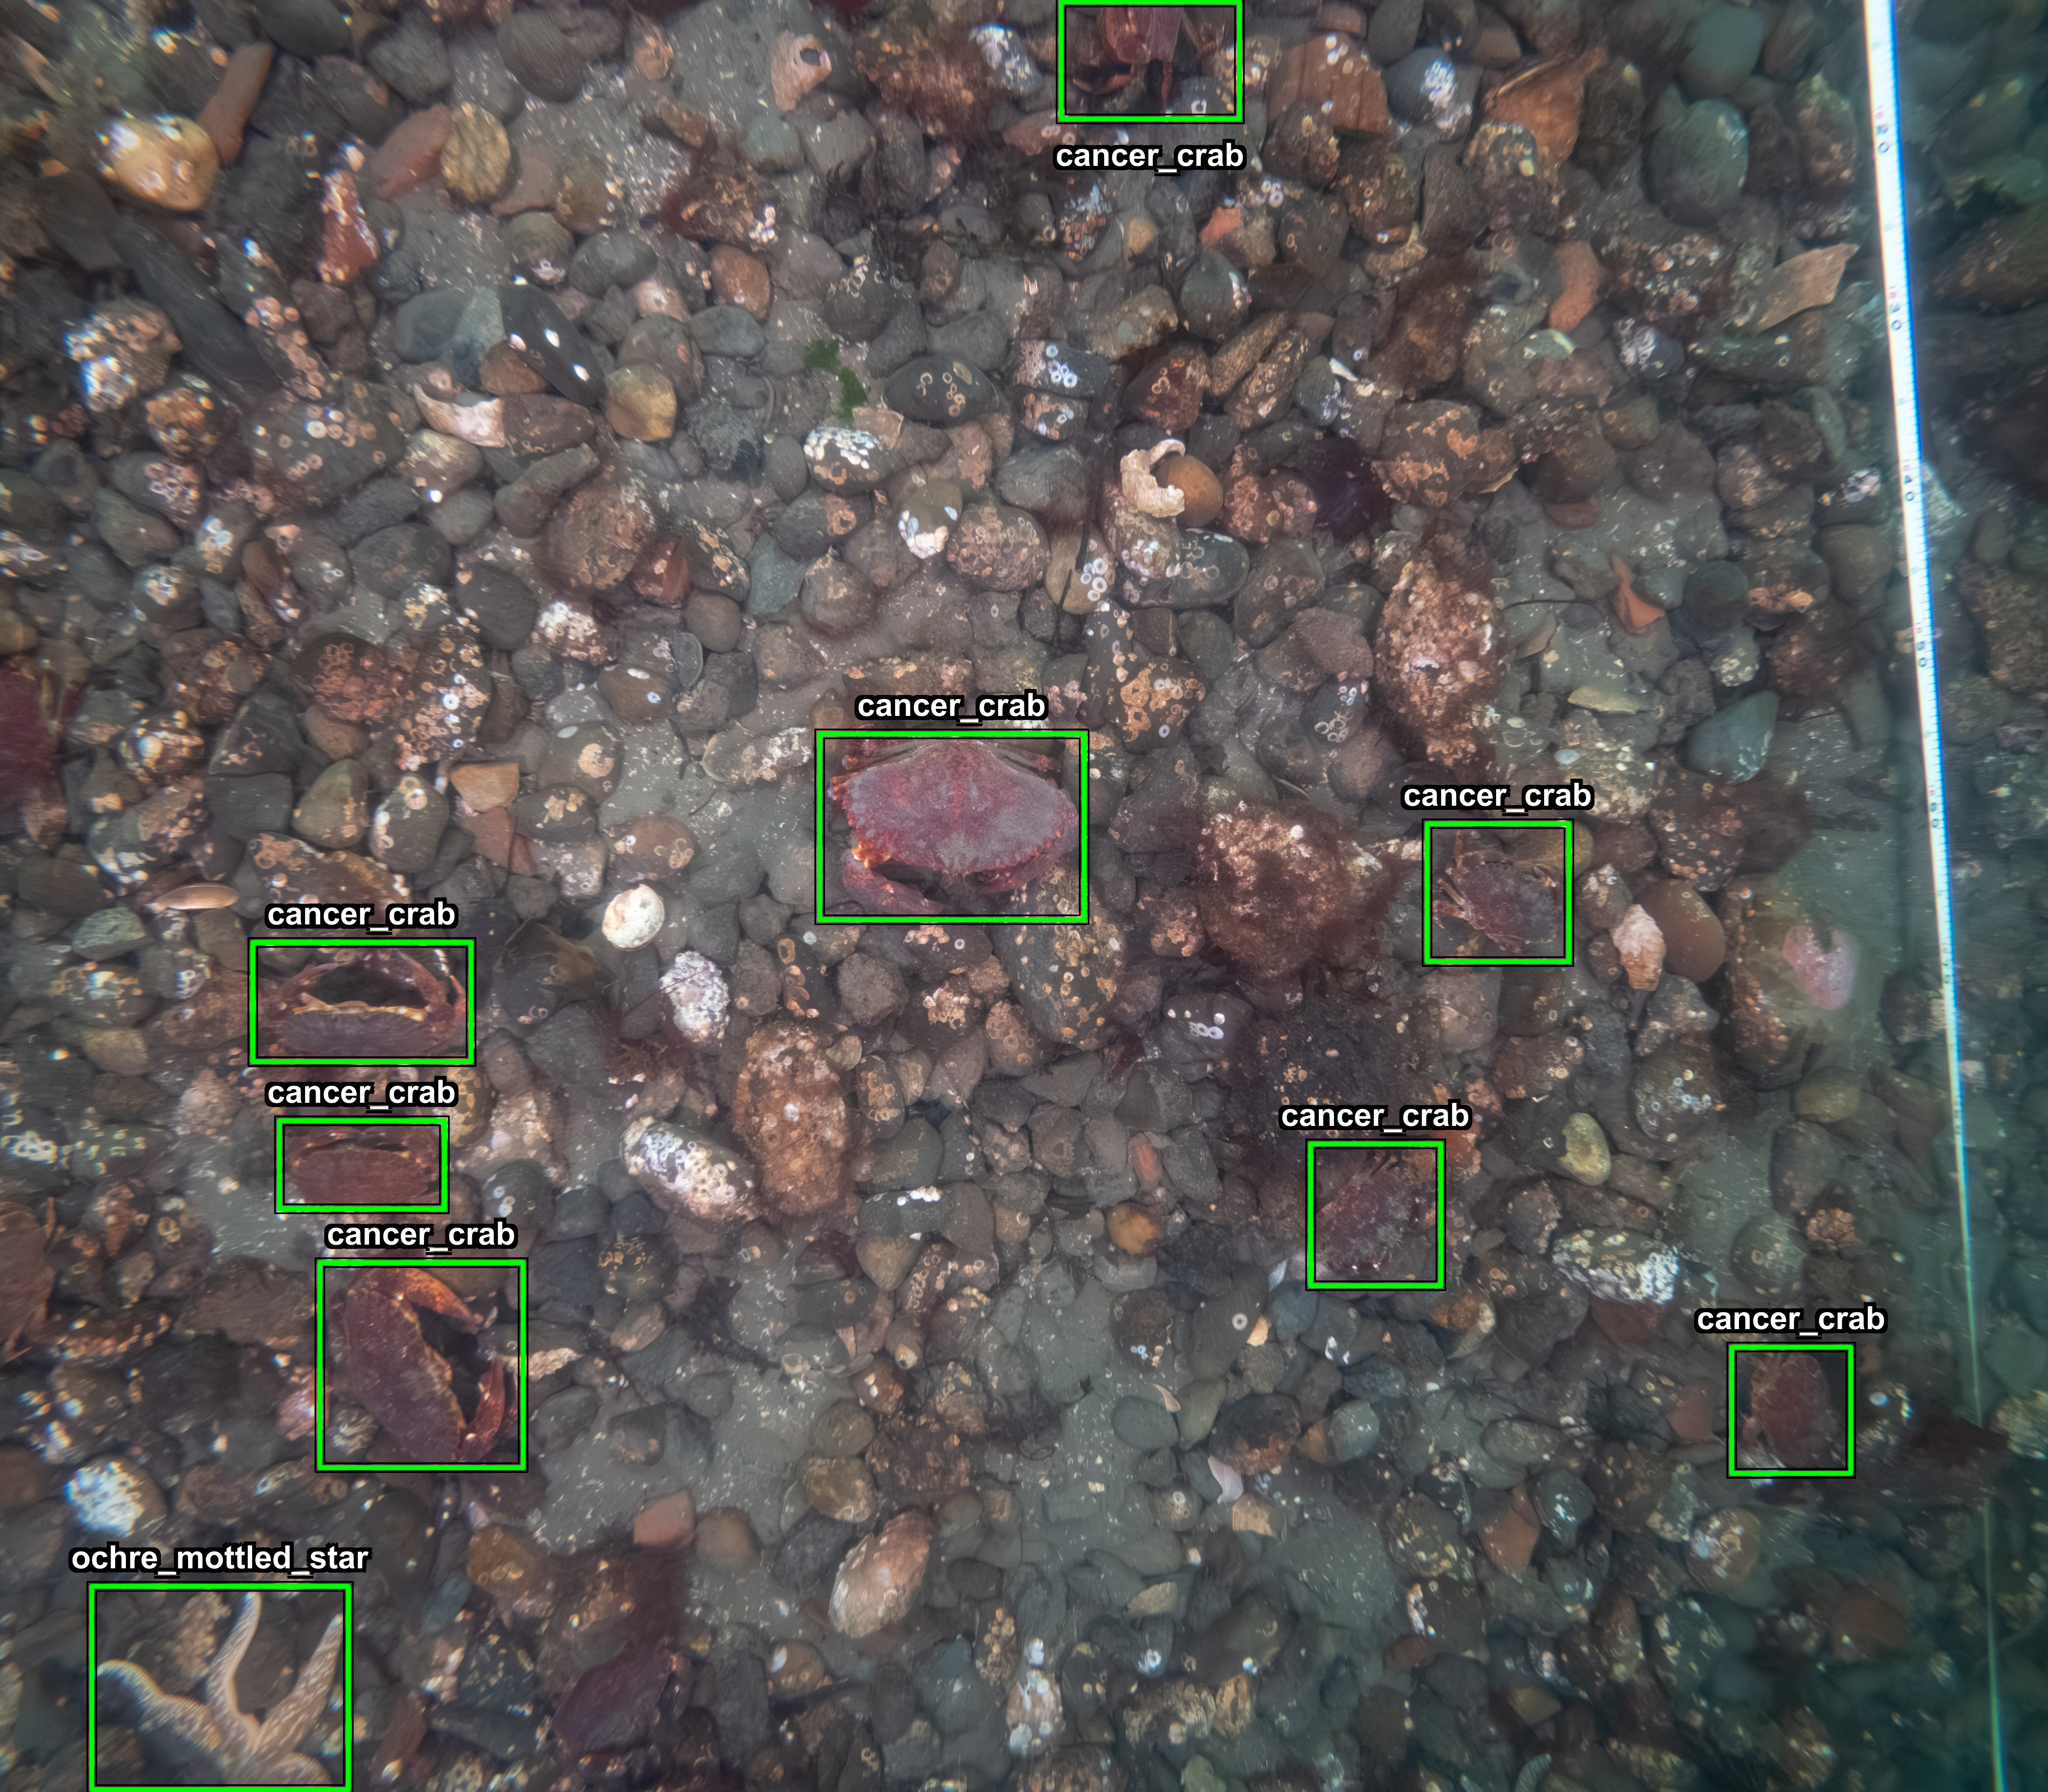
\includegraphics[width=\linewidth]{double_count_4.jpg}
\end{subfigure}%
\hfill%
\begin{subfigure}[t]{0.495\textwidth}
\centering
\textbf{(d)}\par
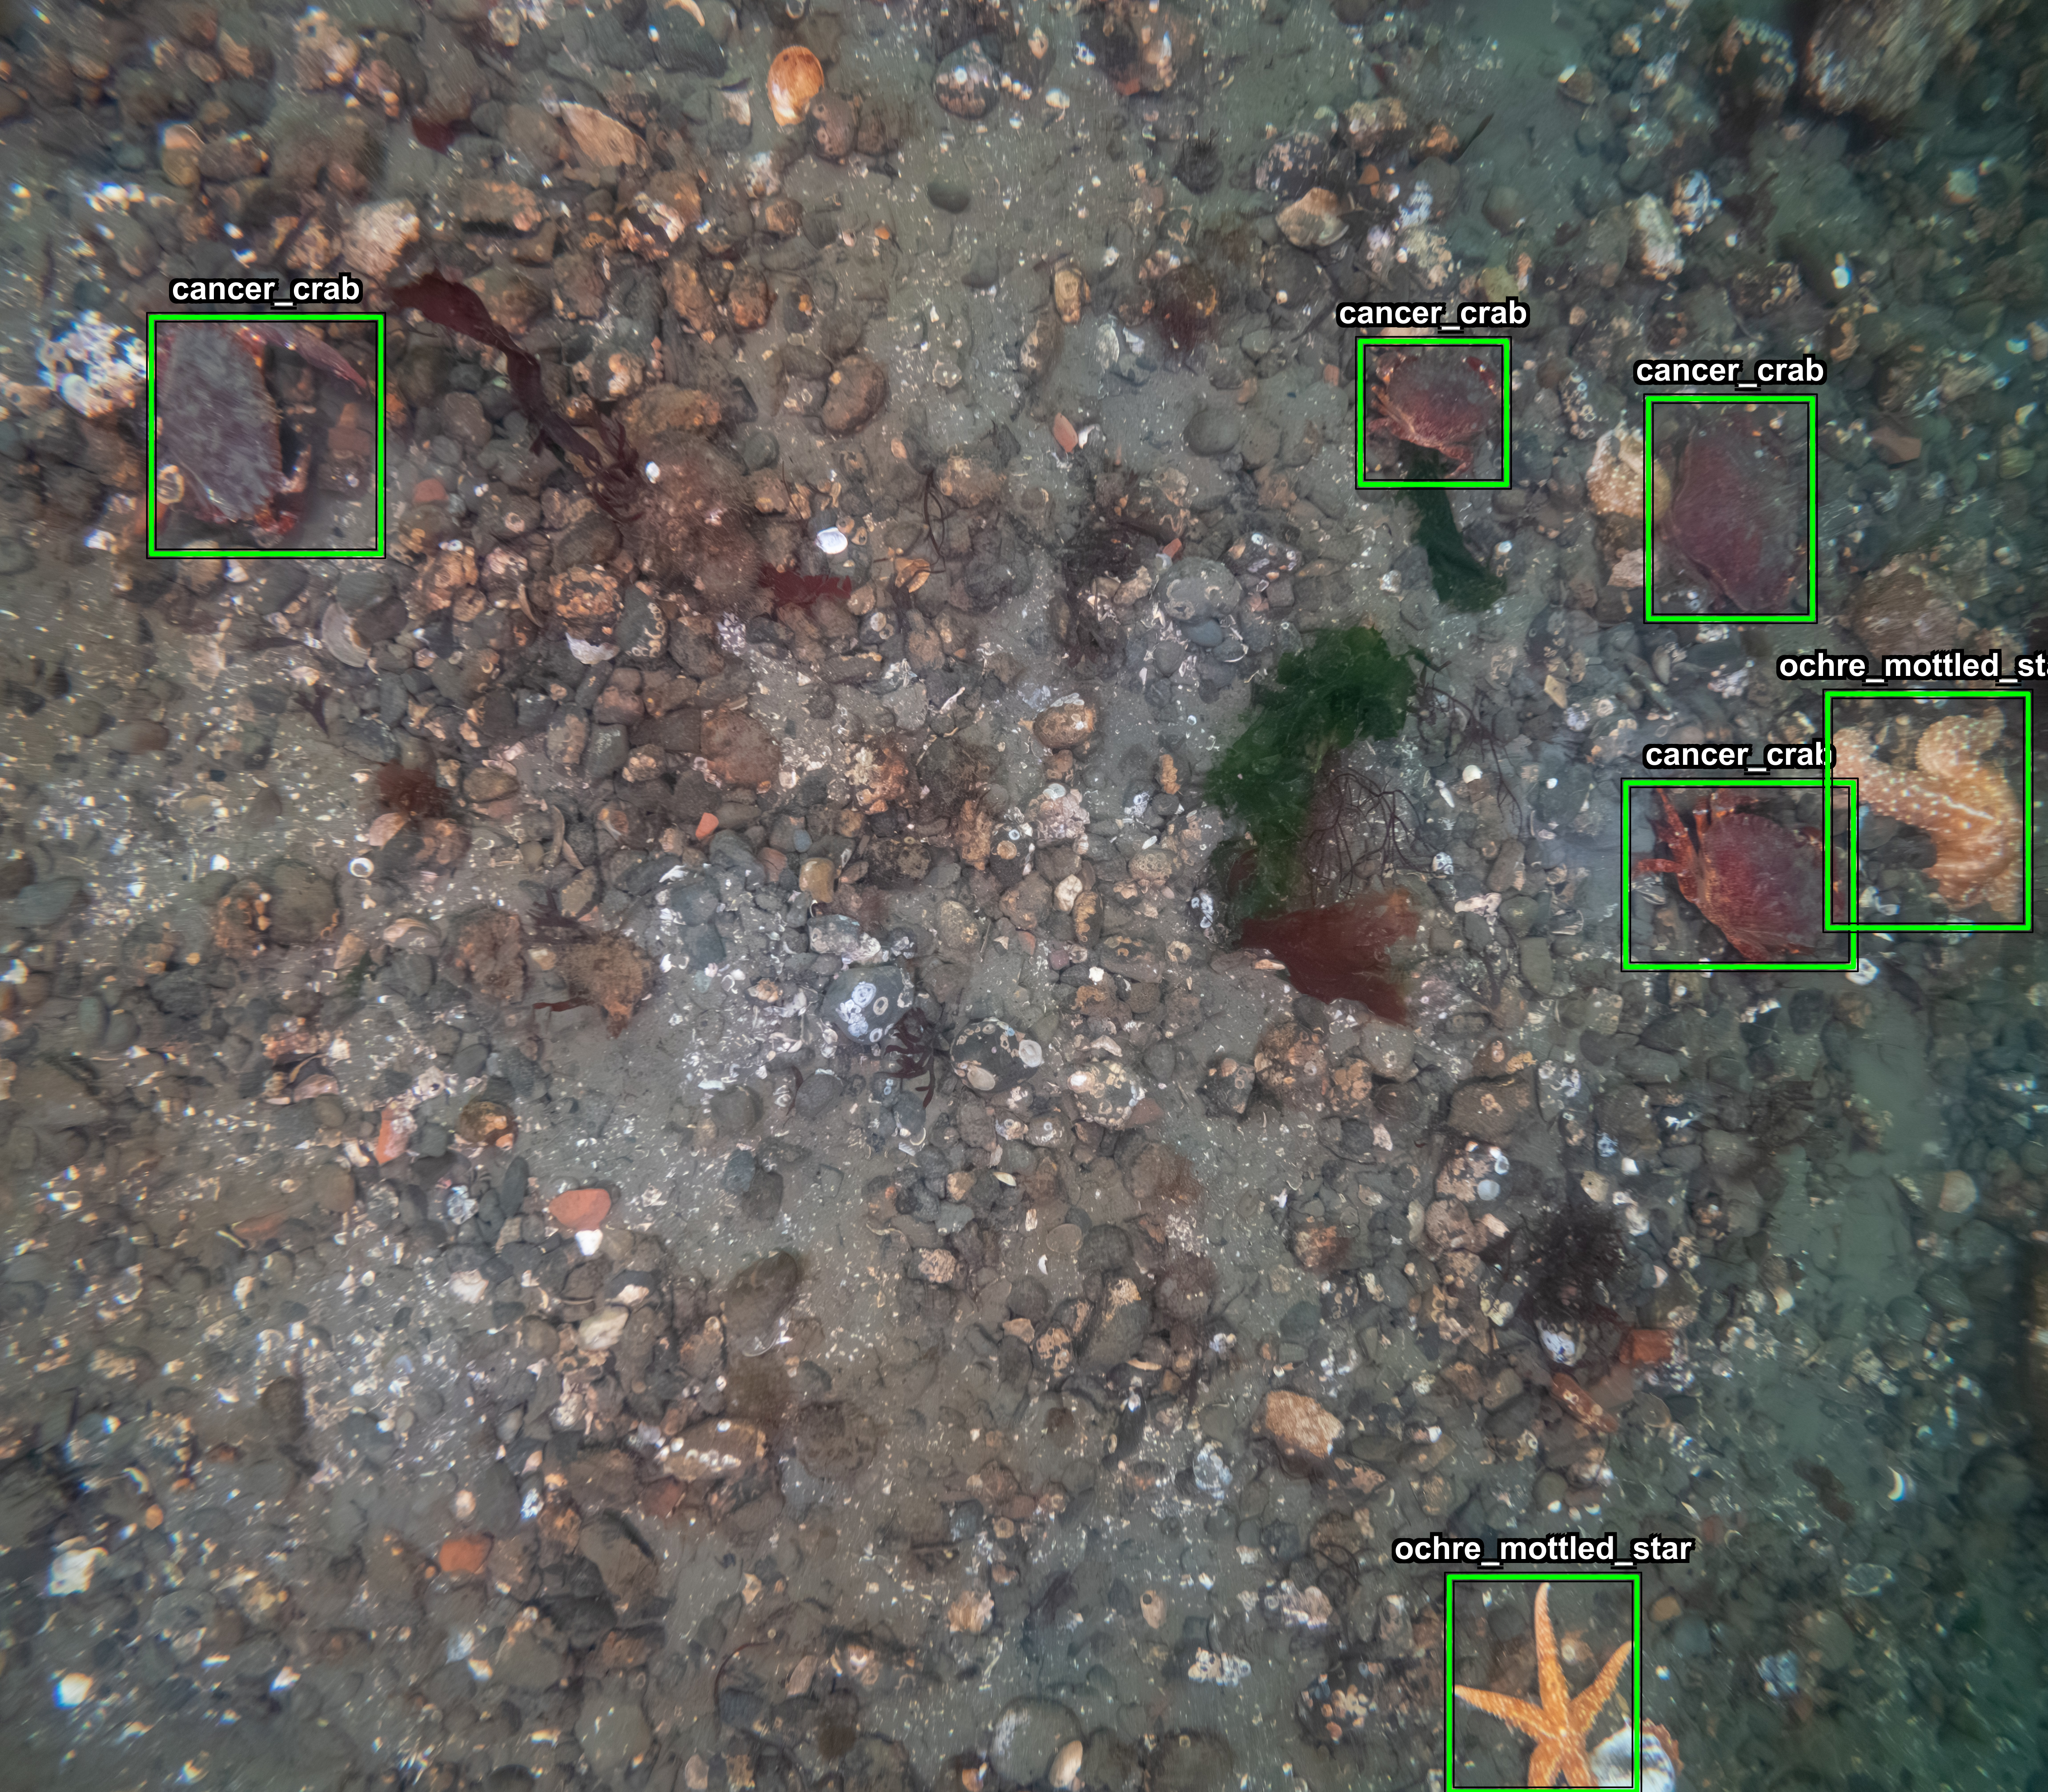
\includegraphics[width=\linewidth]{double_count_2.jpg}
\end{subfigure}
\caption{
Two instances where the ROV ``double-counted'' invertebrates due to the presence
of a slight overlap between sequential ROV survey photographs. 
The rock crab seen at the upper right of (a) is visible once more at the lower 
right of (c);
likewise, the ochre star atop the crab shell debris in the upper right of (b) 
is once more visible at the very bottom right of (d). 
While these instances of image overlap are relatively rare, their influence 
upon double counting invertebrates is clearly density-dependent, as exampled by 
the Centennial Park, winter, T1 transect --- exhibited here --- where clustered
rock crab abundances paired with our sources of error increased the ROV rock
crab abundance total to 130, relative to the diver count of 62.
}
\label{fig:double_count}
\end{figure}
\vfil
}

\clearpage

\vbox to \textheight{%
\vfil
\begin{figure}[H]
\centering
\begin{subfigure}[t]{0.495\textwidth}
\centering
\textbf{(a)}\par
\includegraphics[width=\linewidth]{too_small_1.jpg}
\end{subfigure}%
\hfill%
\begin{subfigure}[t]{0.495\textwidth}
\centering
\textbf{(b)}\par
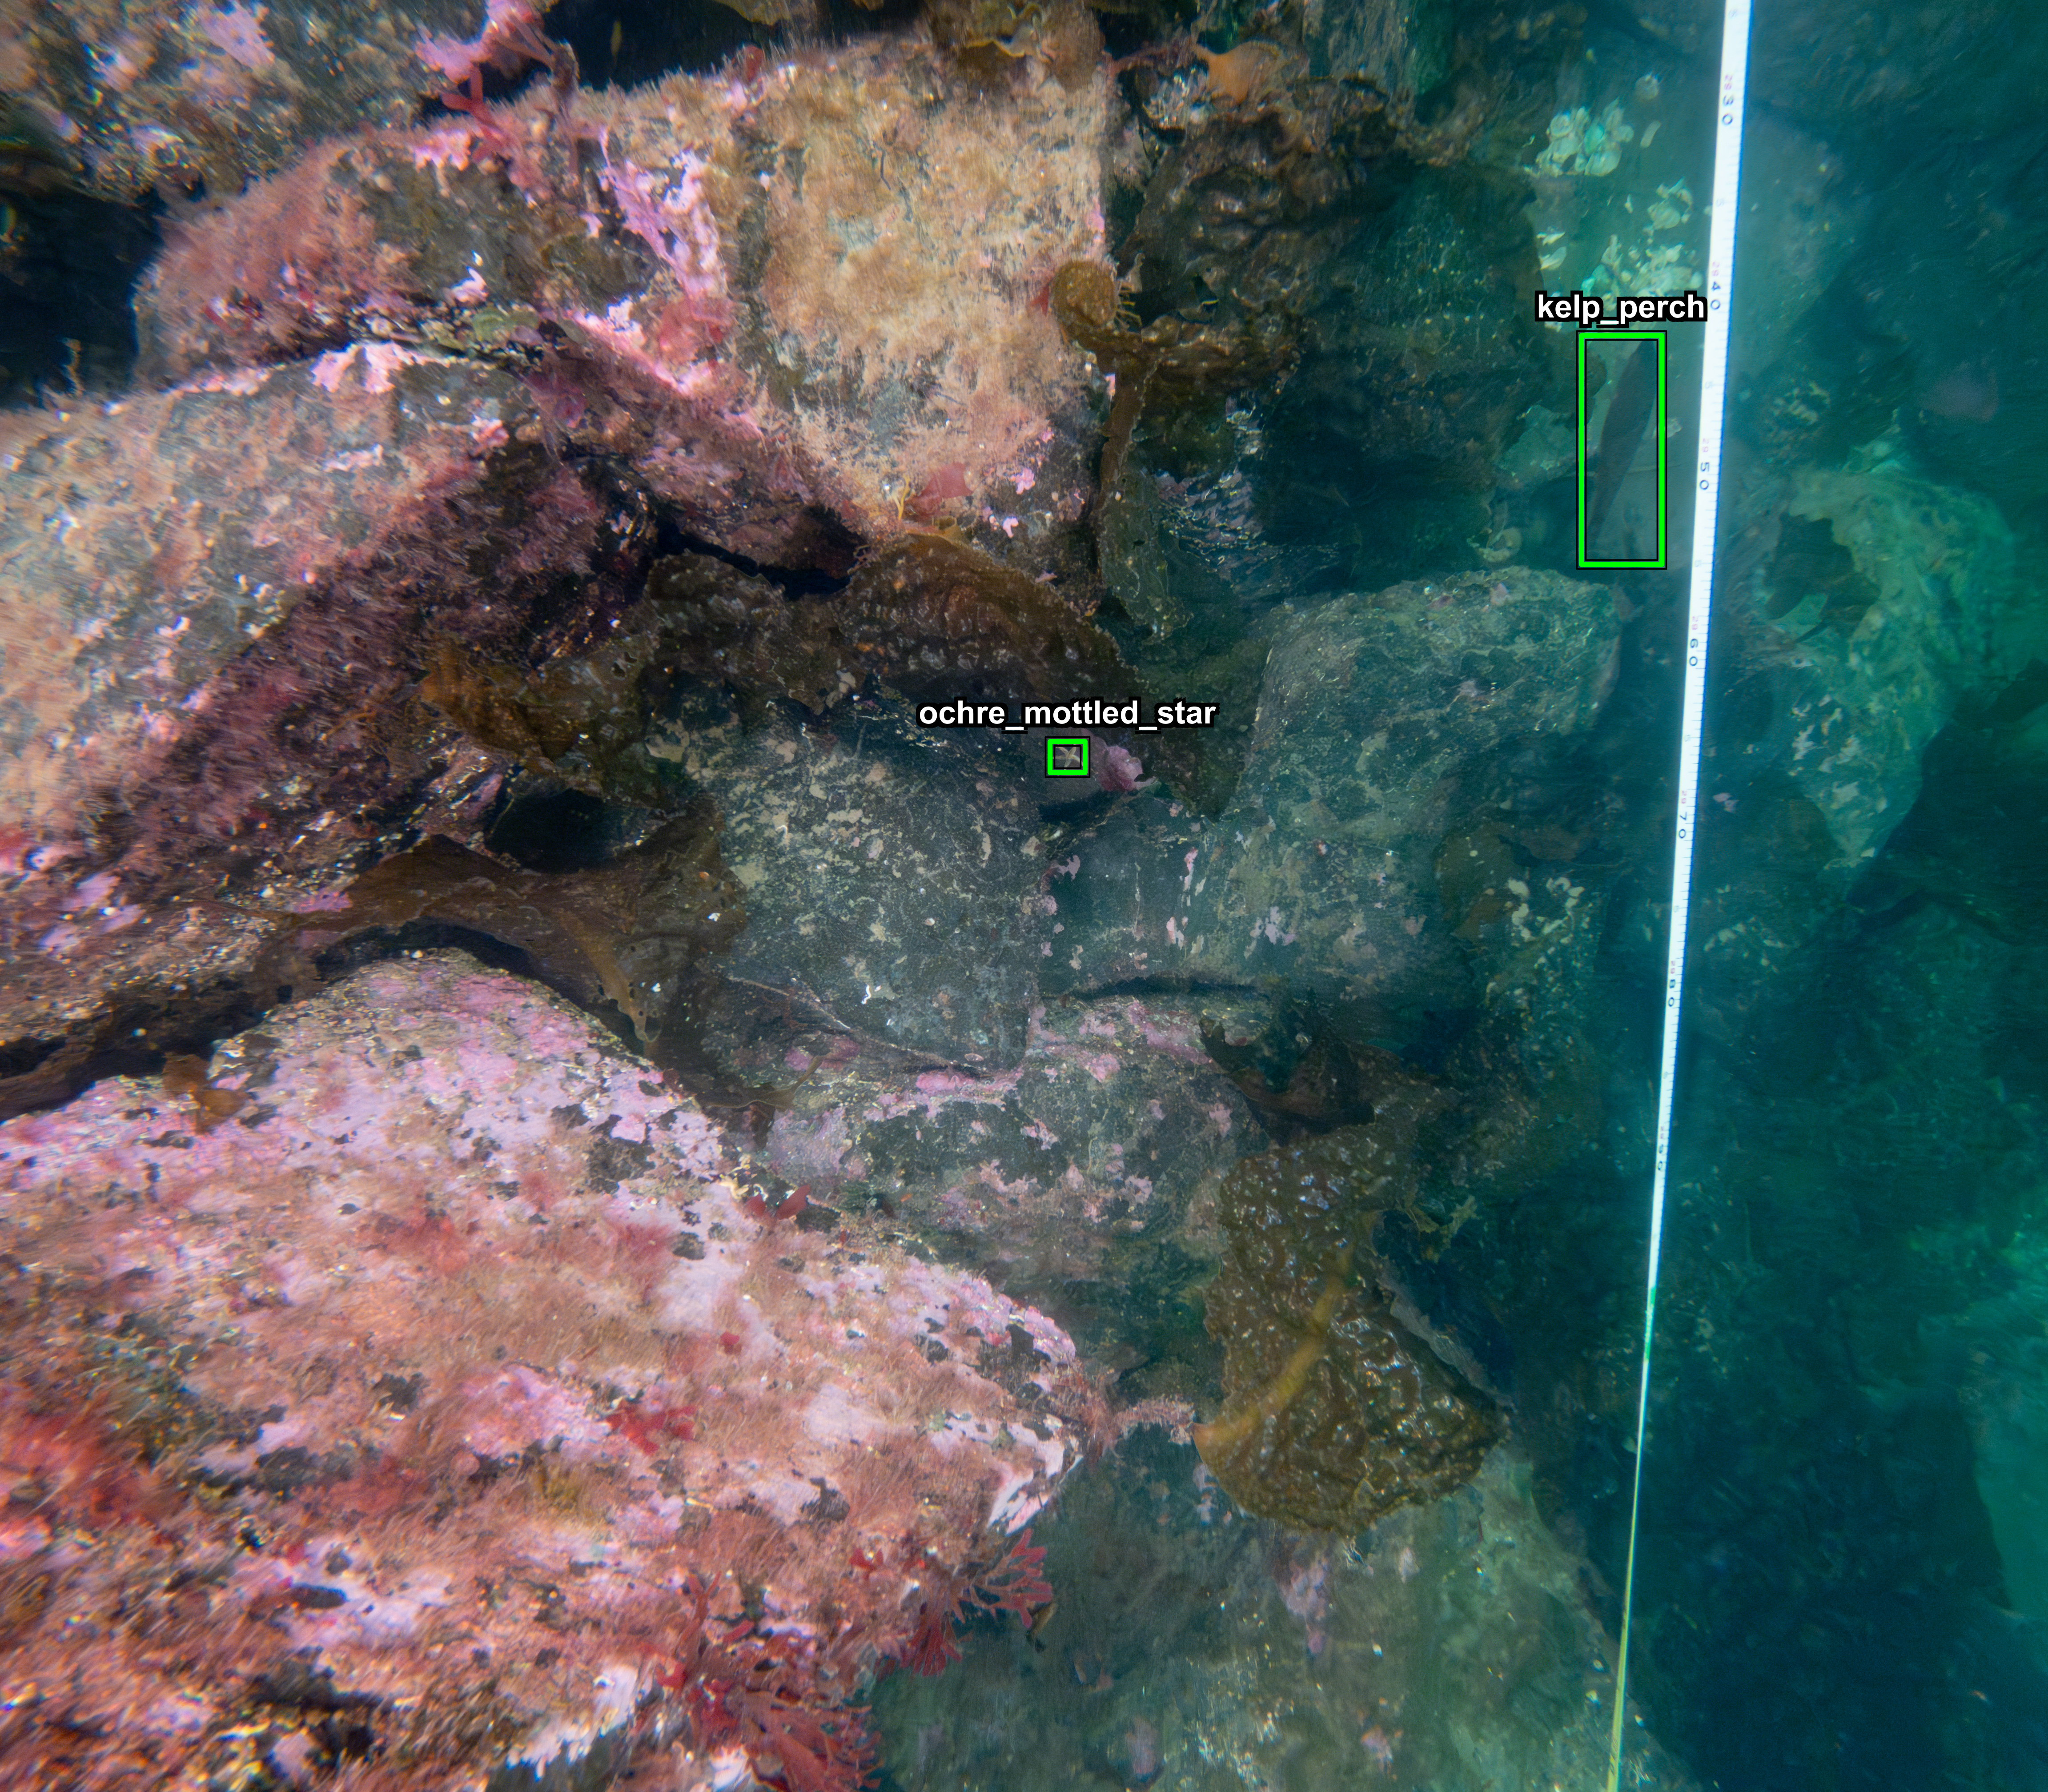
\includegraphics[width=\linewidth]{too_small_2.jpg}
\end{subfigure}
\vspace{0.005\textheight}
\begin{subfigure}[t]{0.495\textwidth}
\centering
\textbf{(c)}\par
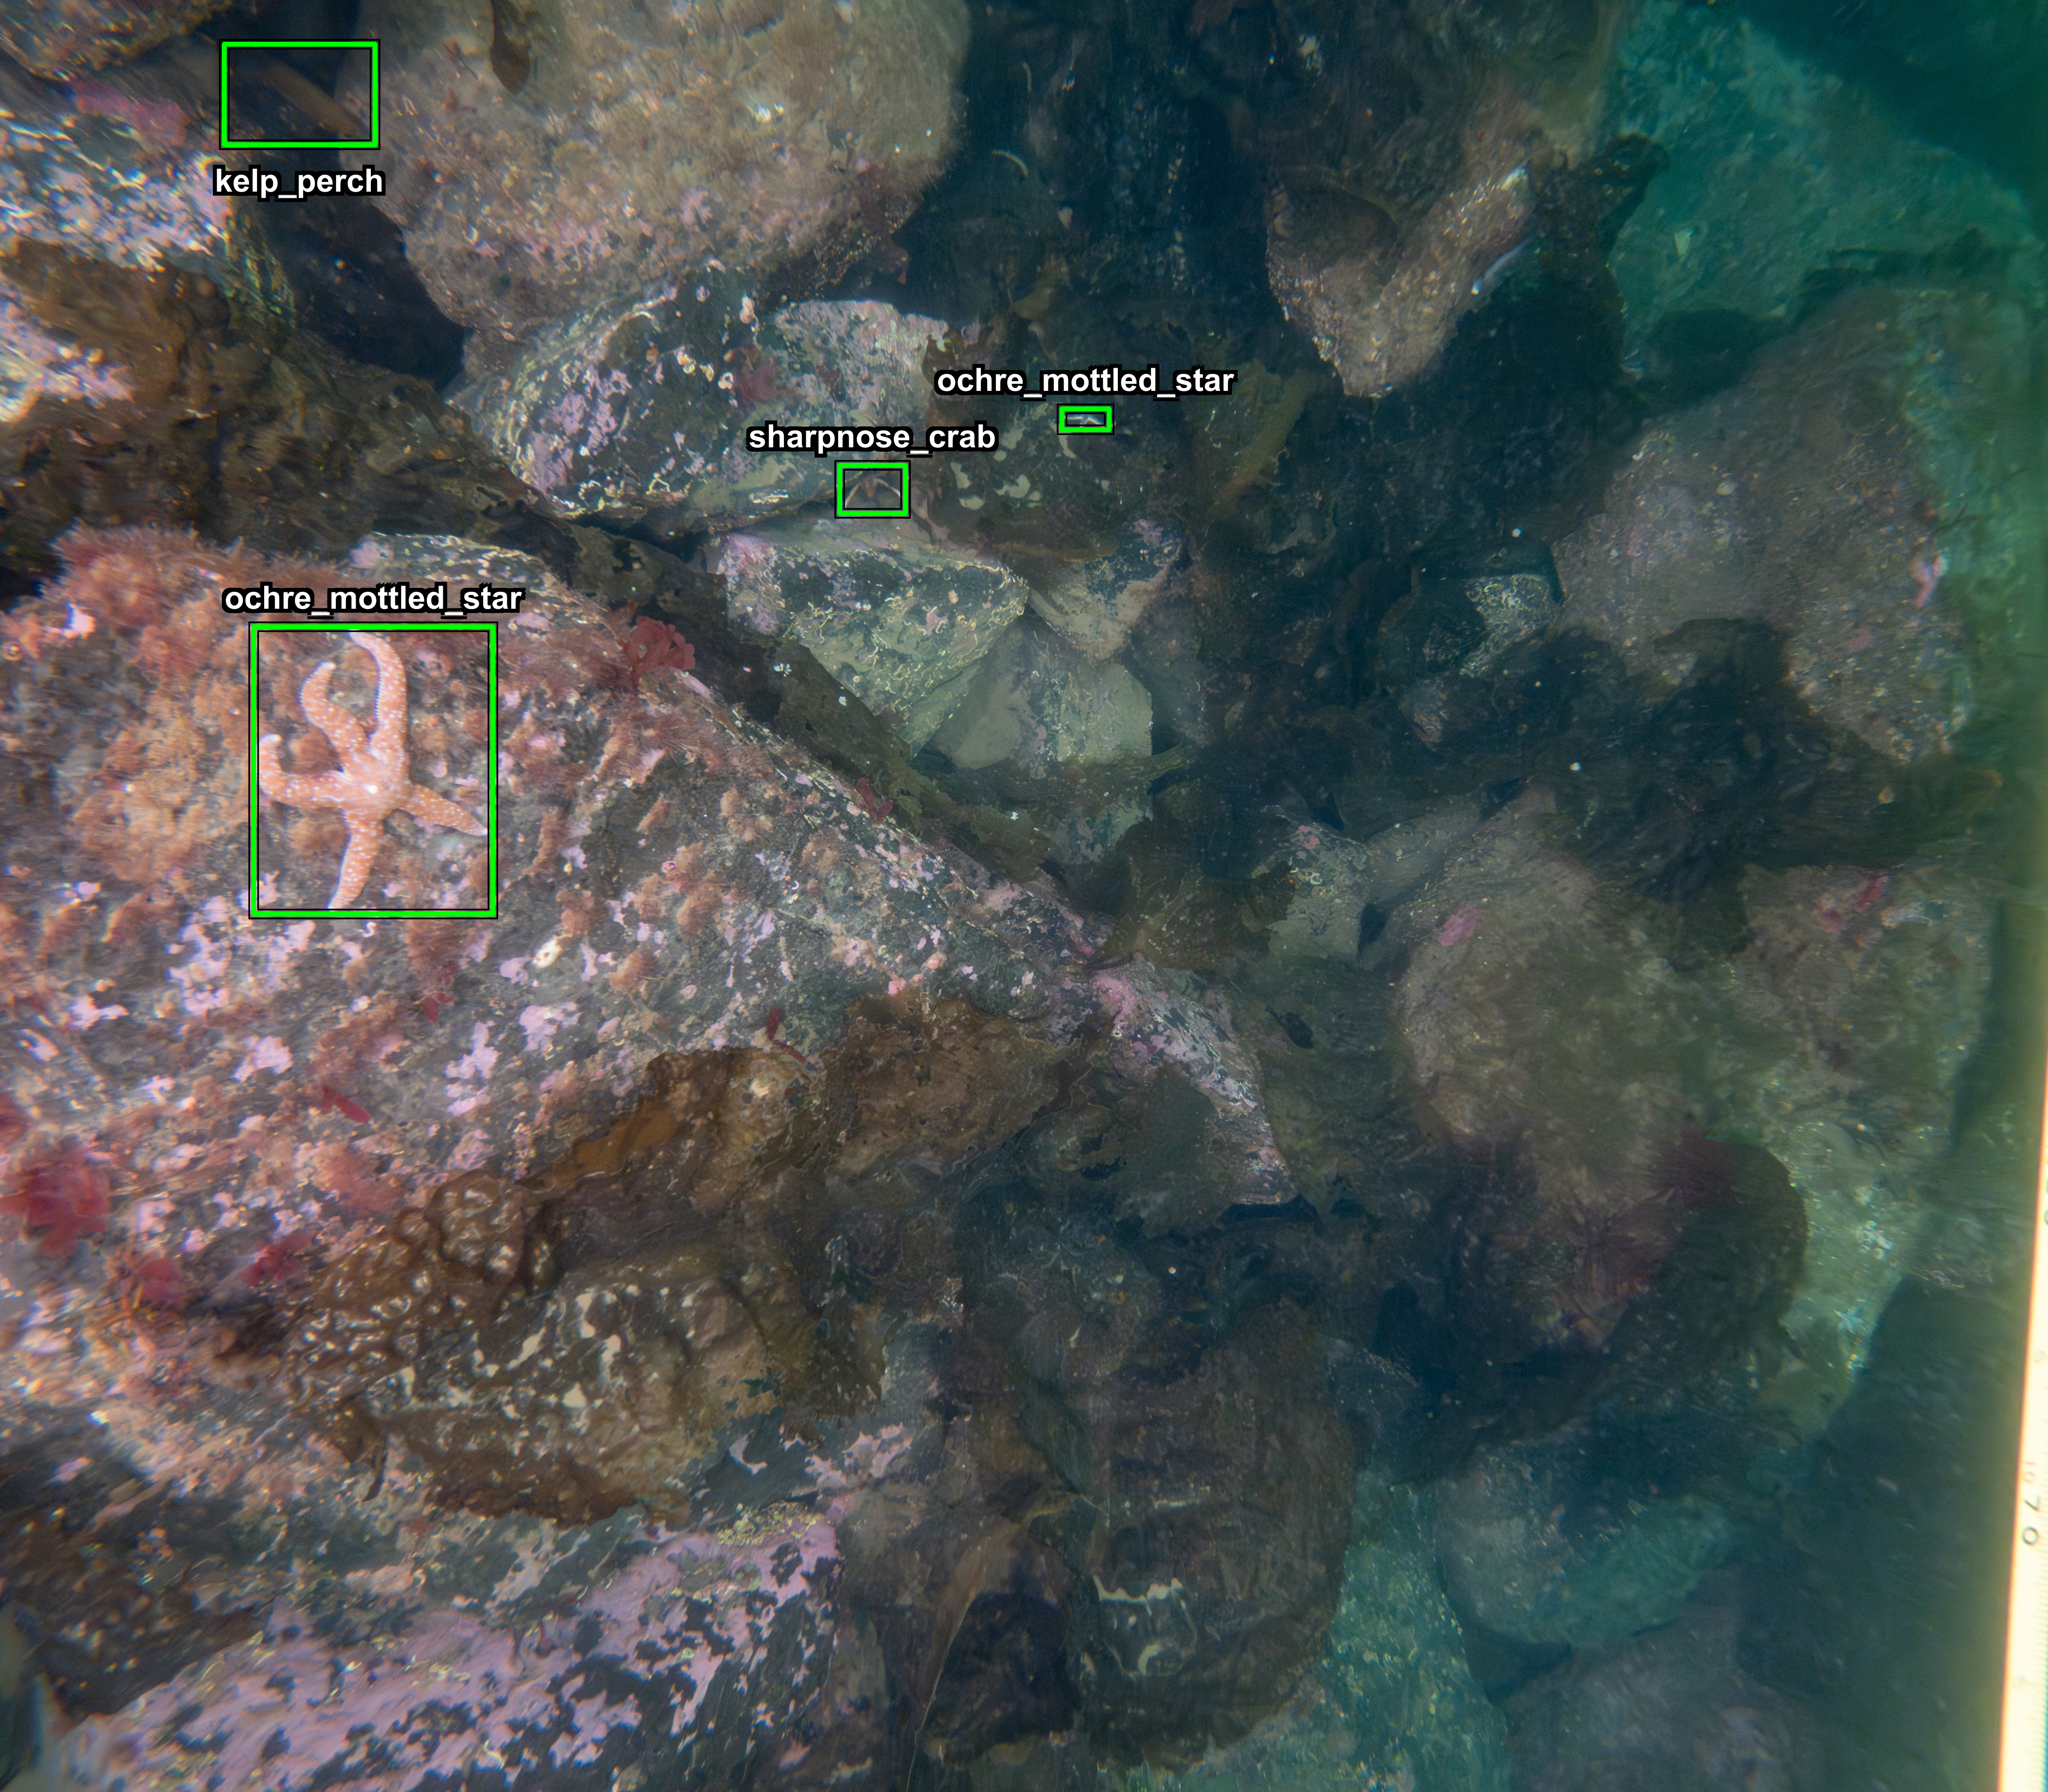
\includegraphics[width=\linewidth]{too_small_3.jpg}
\end{subfigure}%
\hfill%
\begin{subfigure}[t]{0.495\textwidth}
\centering
\textbf{(d)}\par
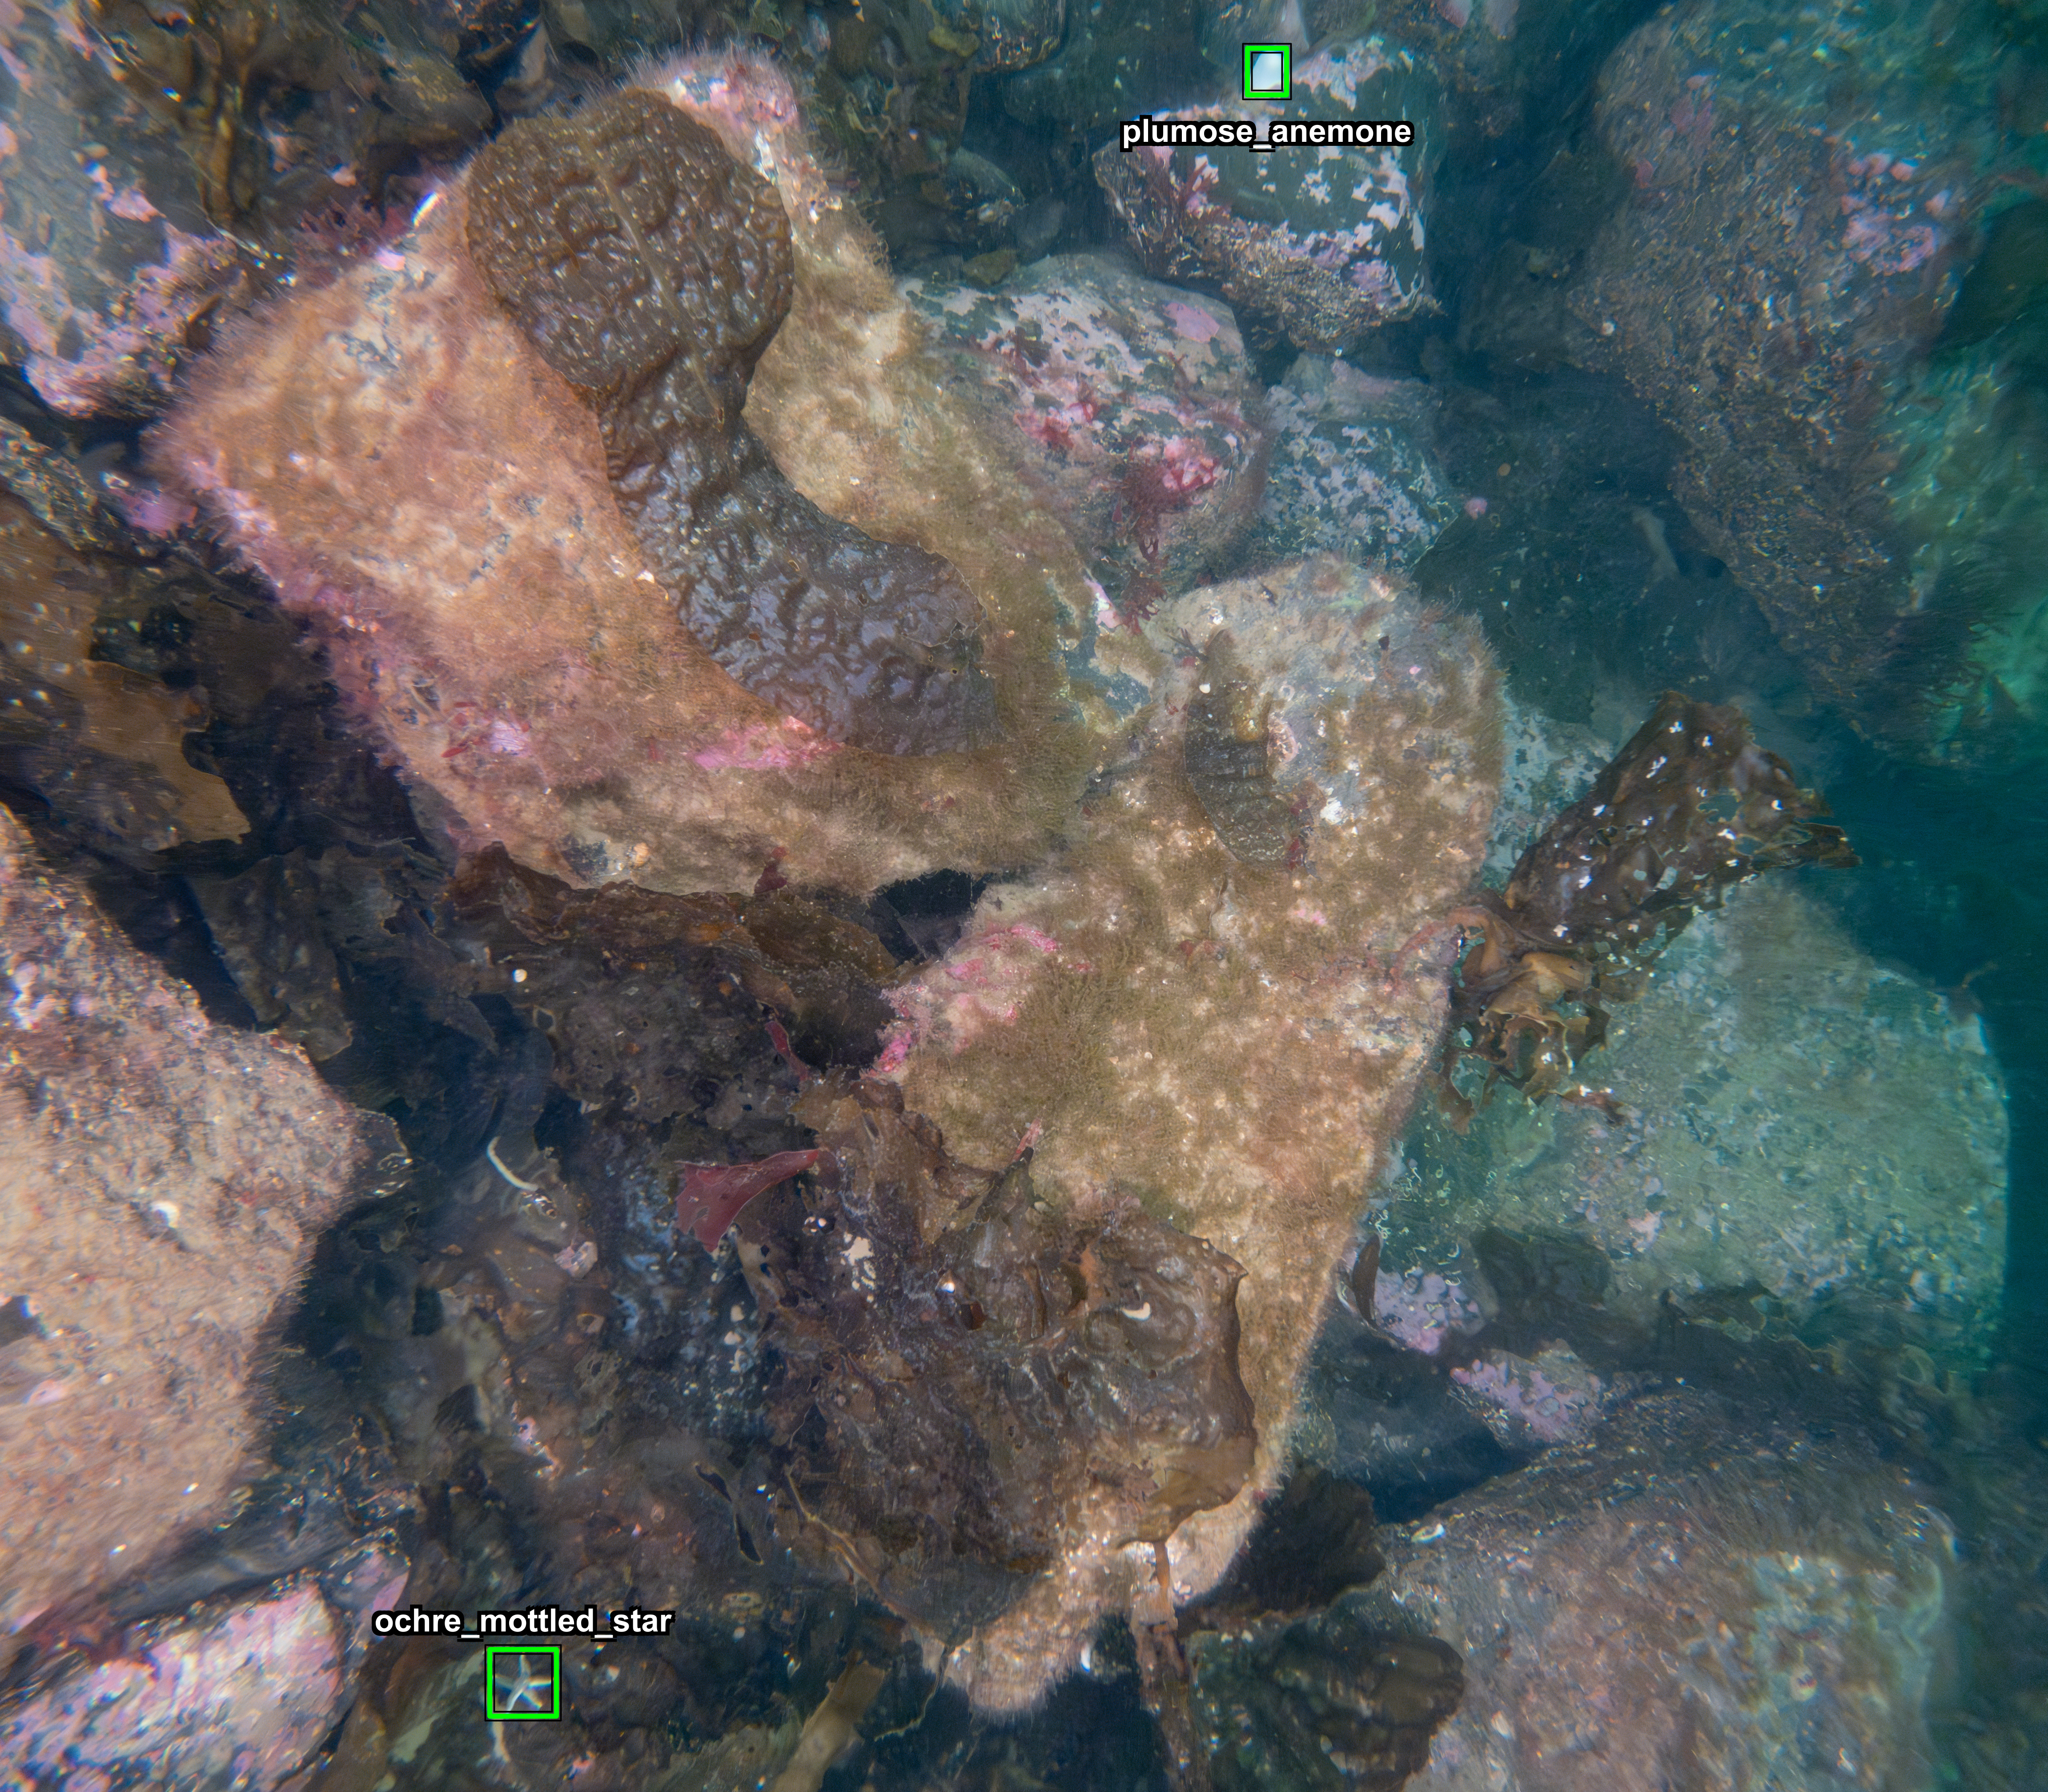
\includegraphics[width=\linewidth]{too_small_4.jpg}
\end{subfigure}
\caption{
While relatively rare, there were several instances where the ROV --- as it 
does not have a scale metric for its downward-facing photographs --- generated 
annotations for invertebrates that likely exhibited a diameter $\le~2.5~cm$, 
below the cut-off used by Reef Check divers to count an invertebrate. 
Each image above depicts at least one instance of these very small 
invertebrates. 
}
\label{fig:too_small}
\end{figure}
\vfil
}

\clearpage

\vbox to \textheight{%
\vfil
\begin{figure}[H]
\centering
\begin{subfigure}[t]{0.495\textwidth}
\centering
\textbf{(a)}\par
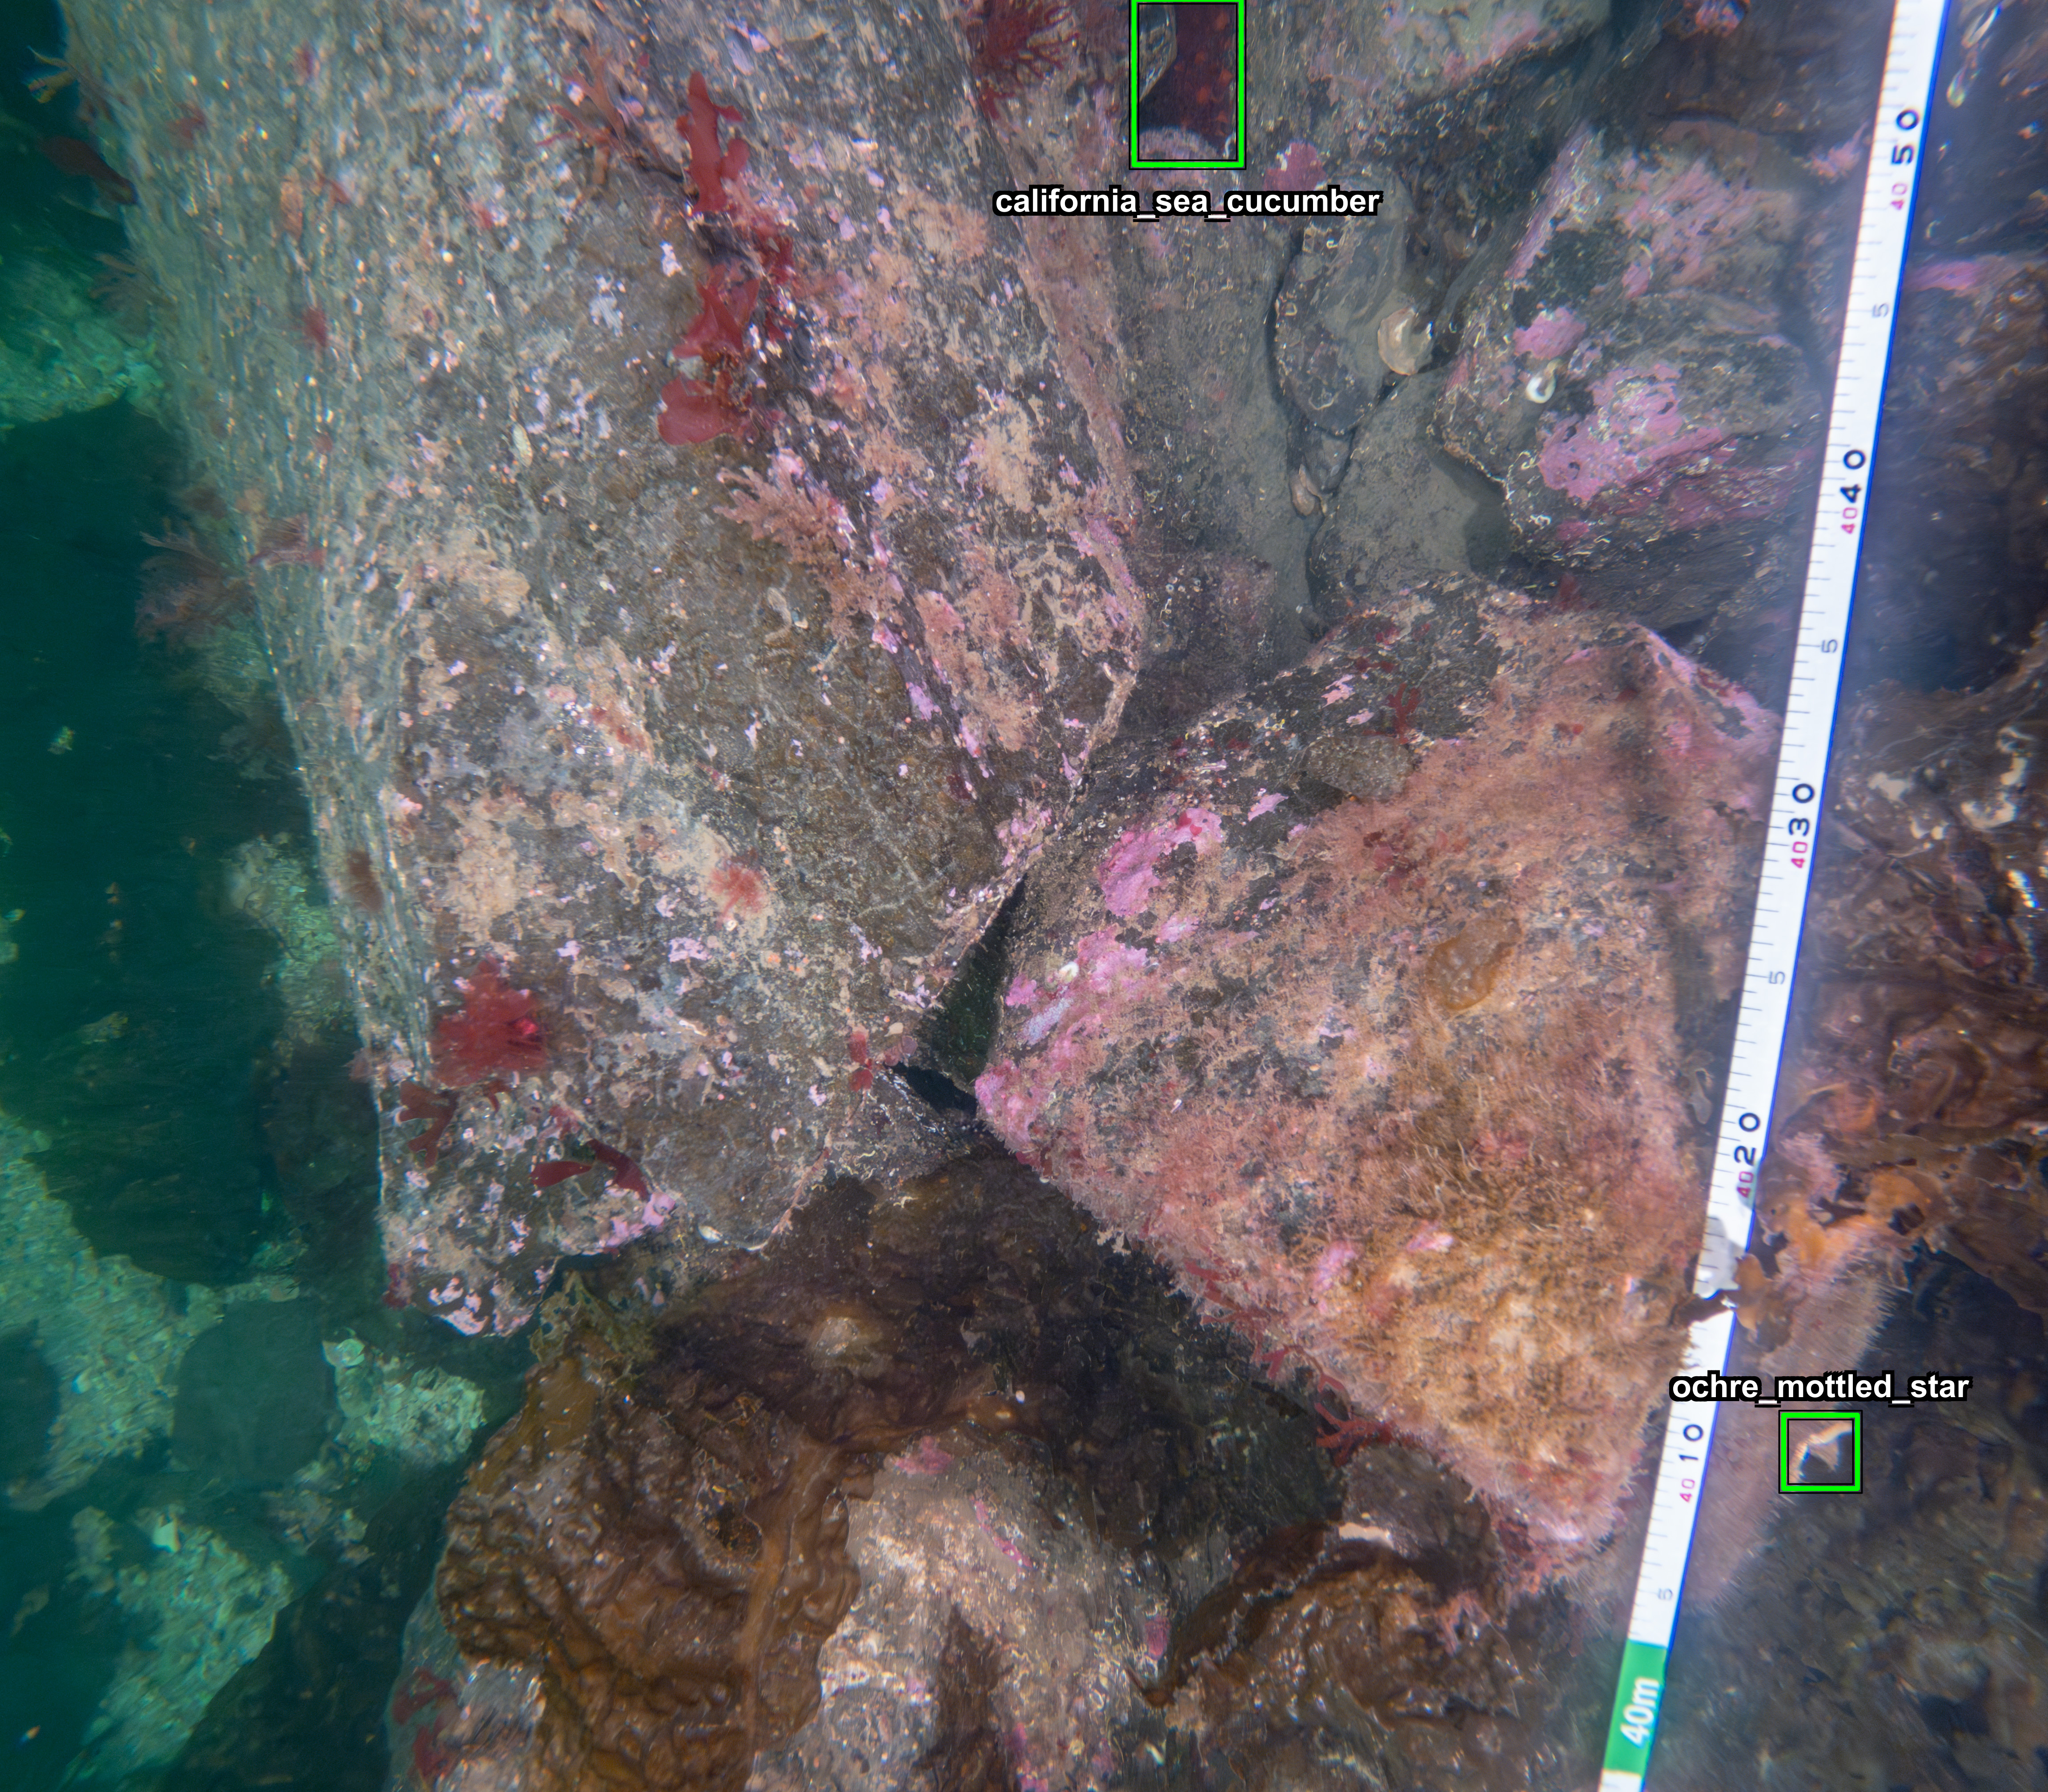
\includegraphics[width=\linewidth]{off_sides_1.jpg}
\end{subfigure}%
\hfill%
\begin{subfigure}[t]{0.495\textwidth}
\centering
\textbf{(b)}\par
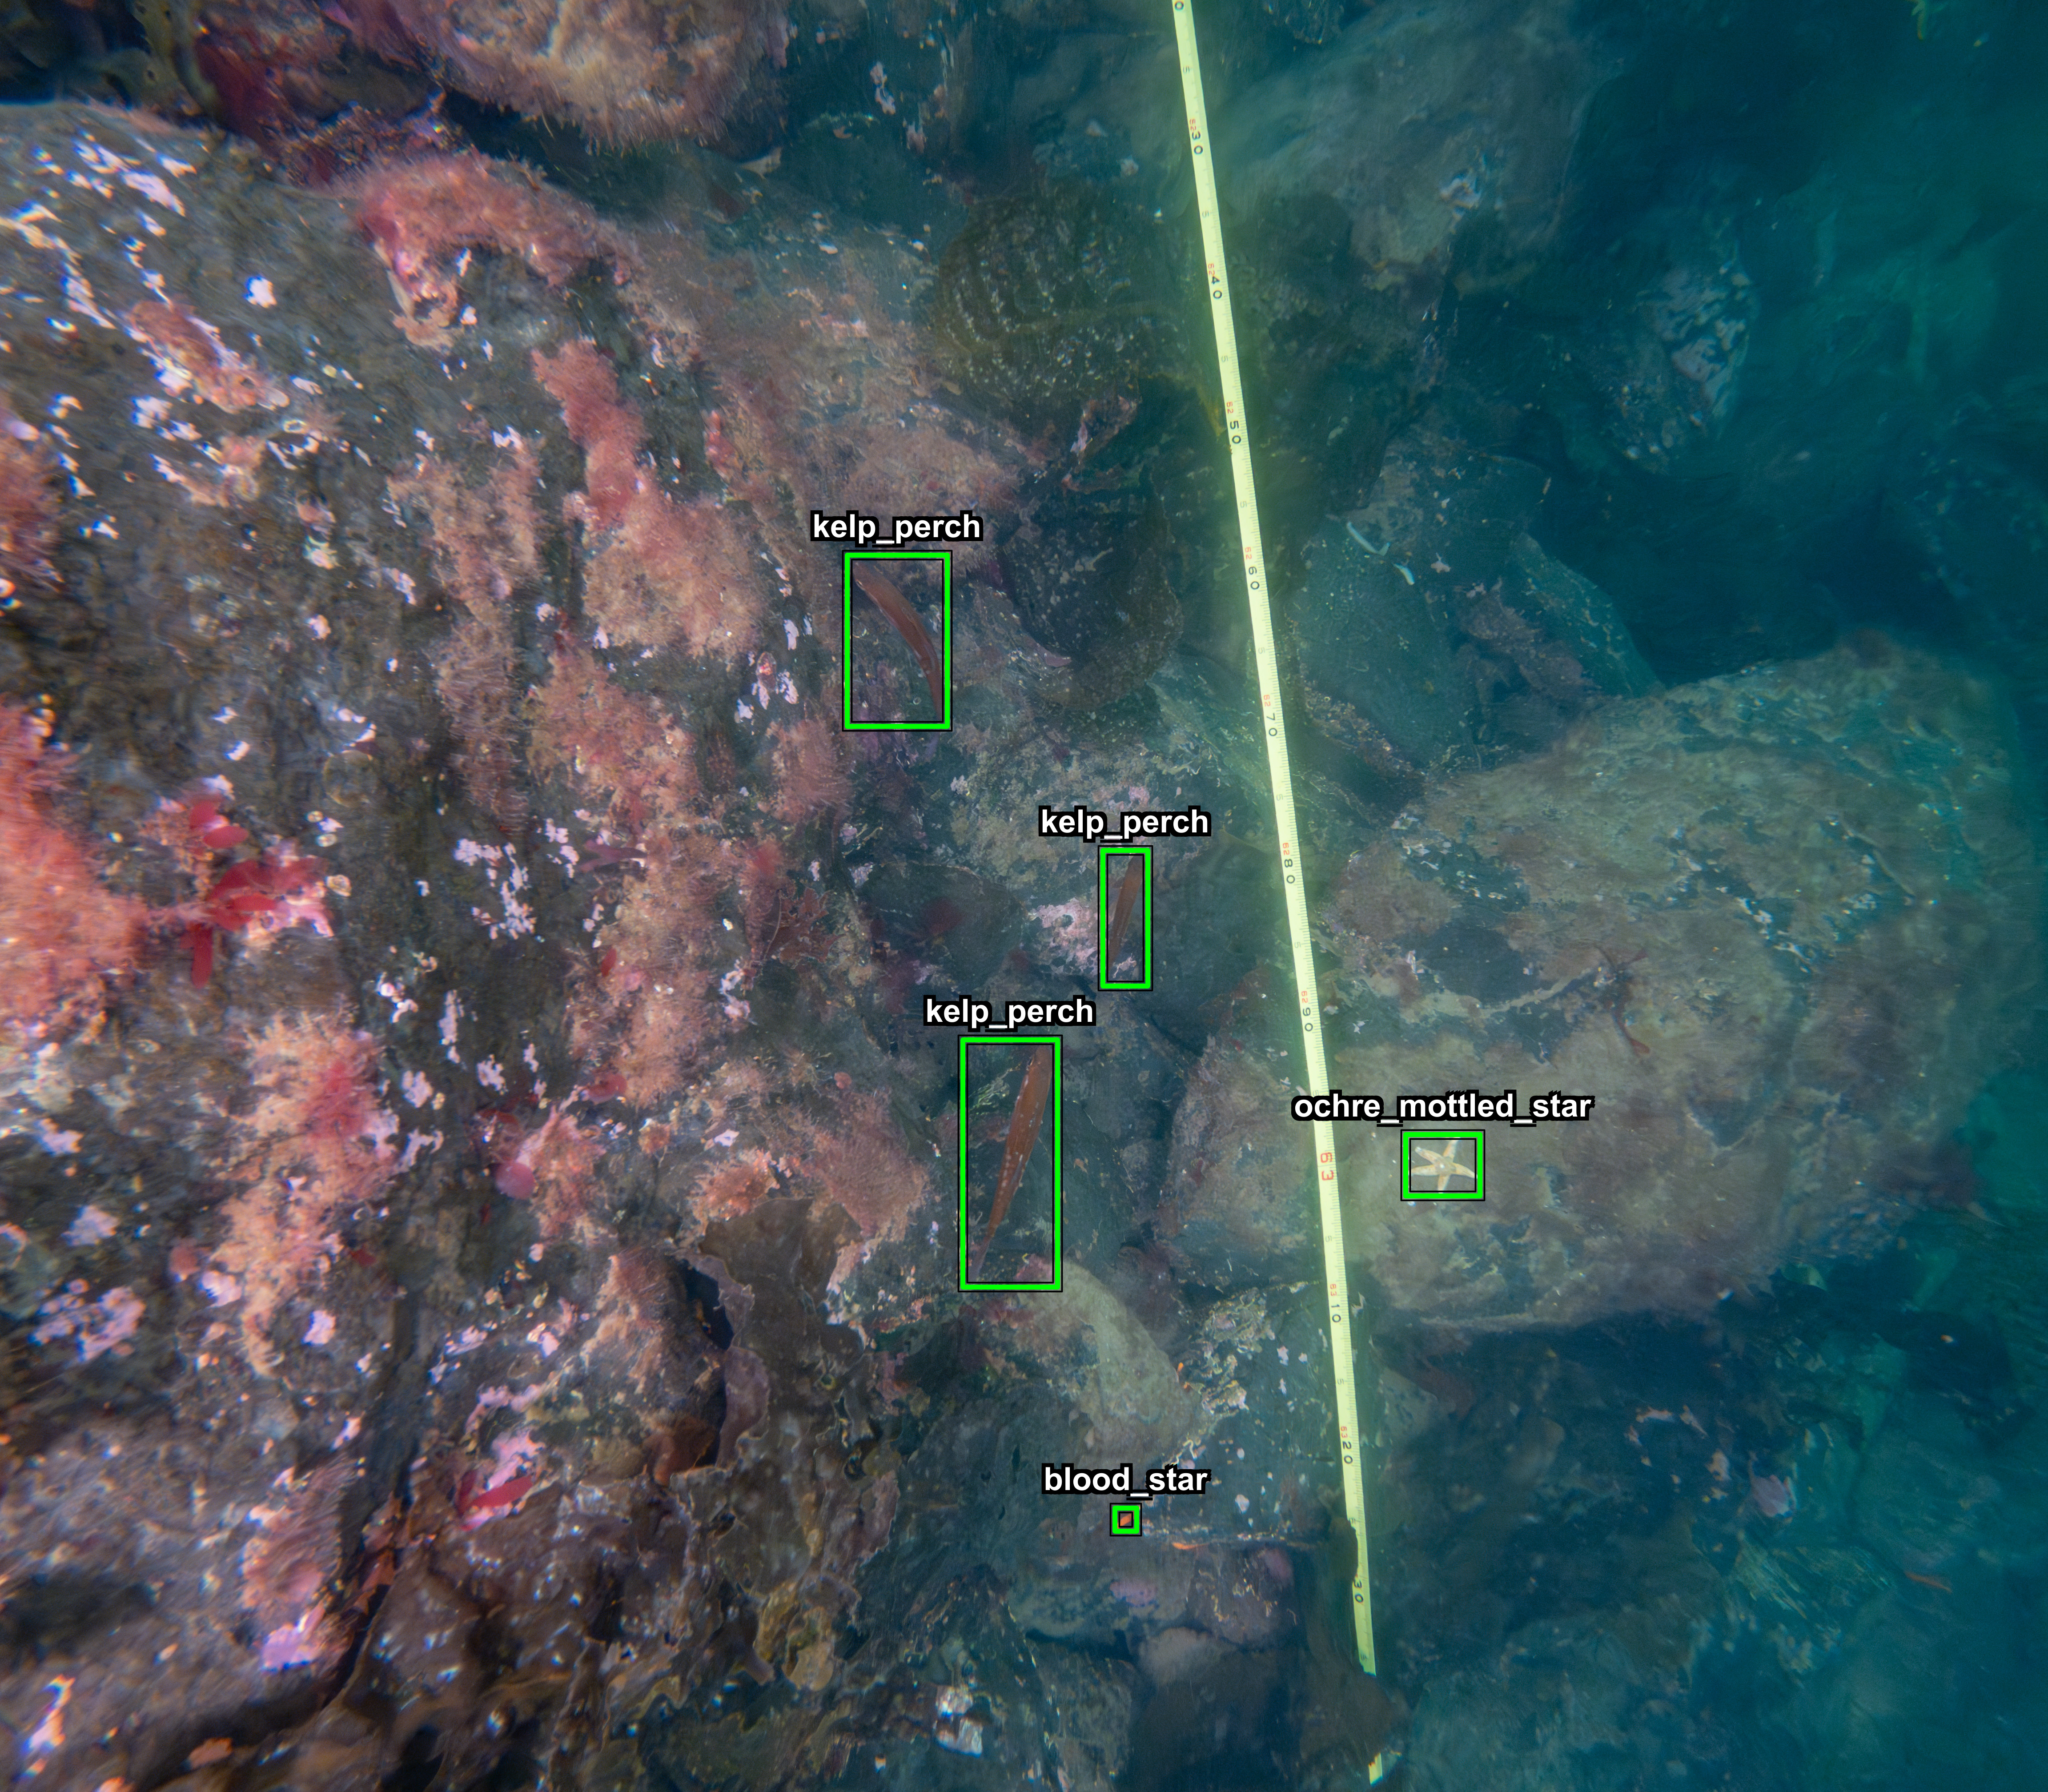
\includegraphics[width=\linewidth]{off_sides_2.jpg}
\end{subfigure}
\vspace{0.005\textheight}
\begin{subfigure}[t]{0.495\textwidth}
\centering
\textbf{(c)}\par
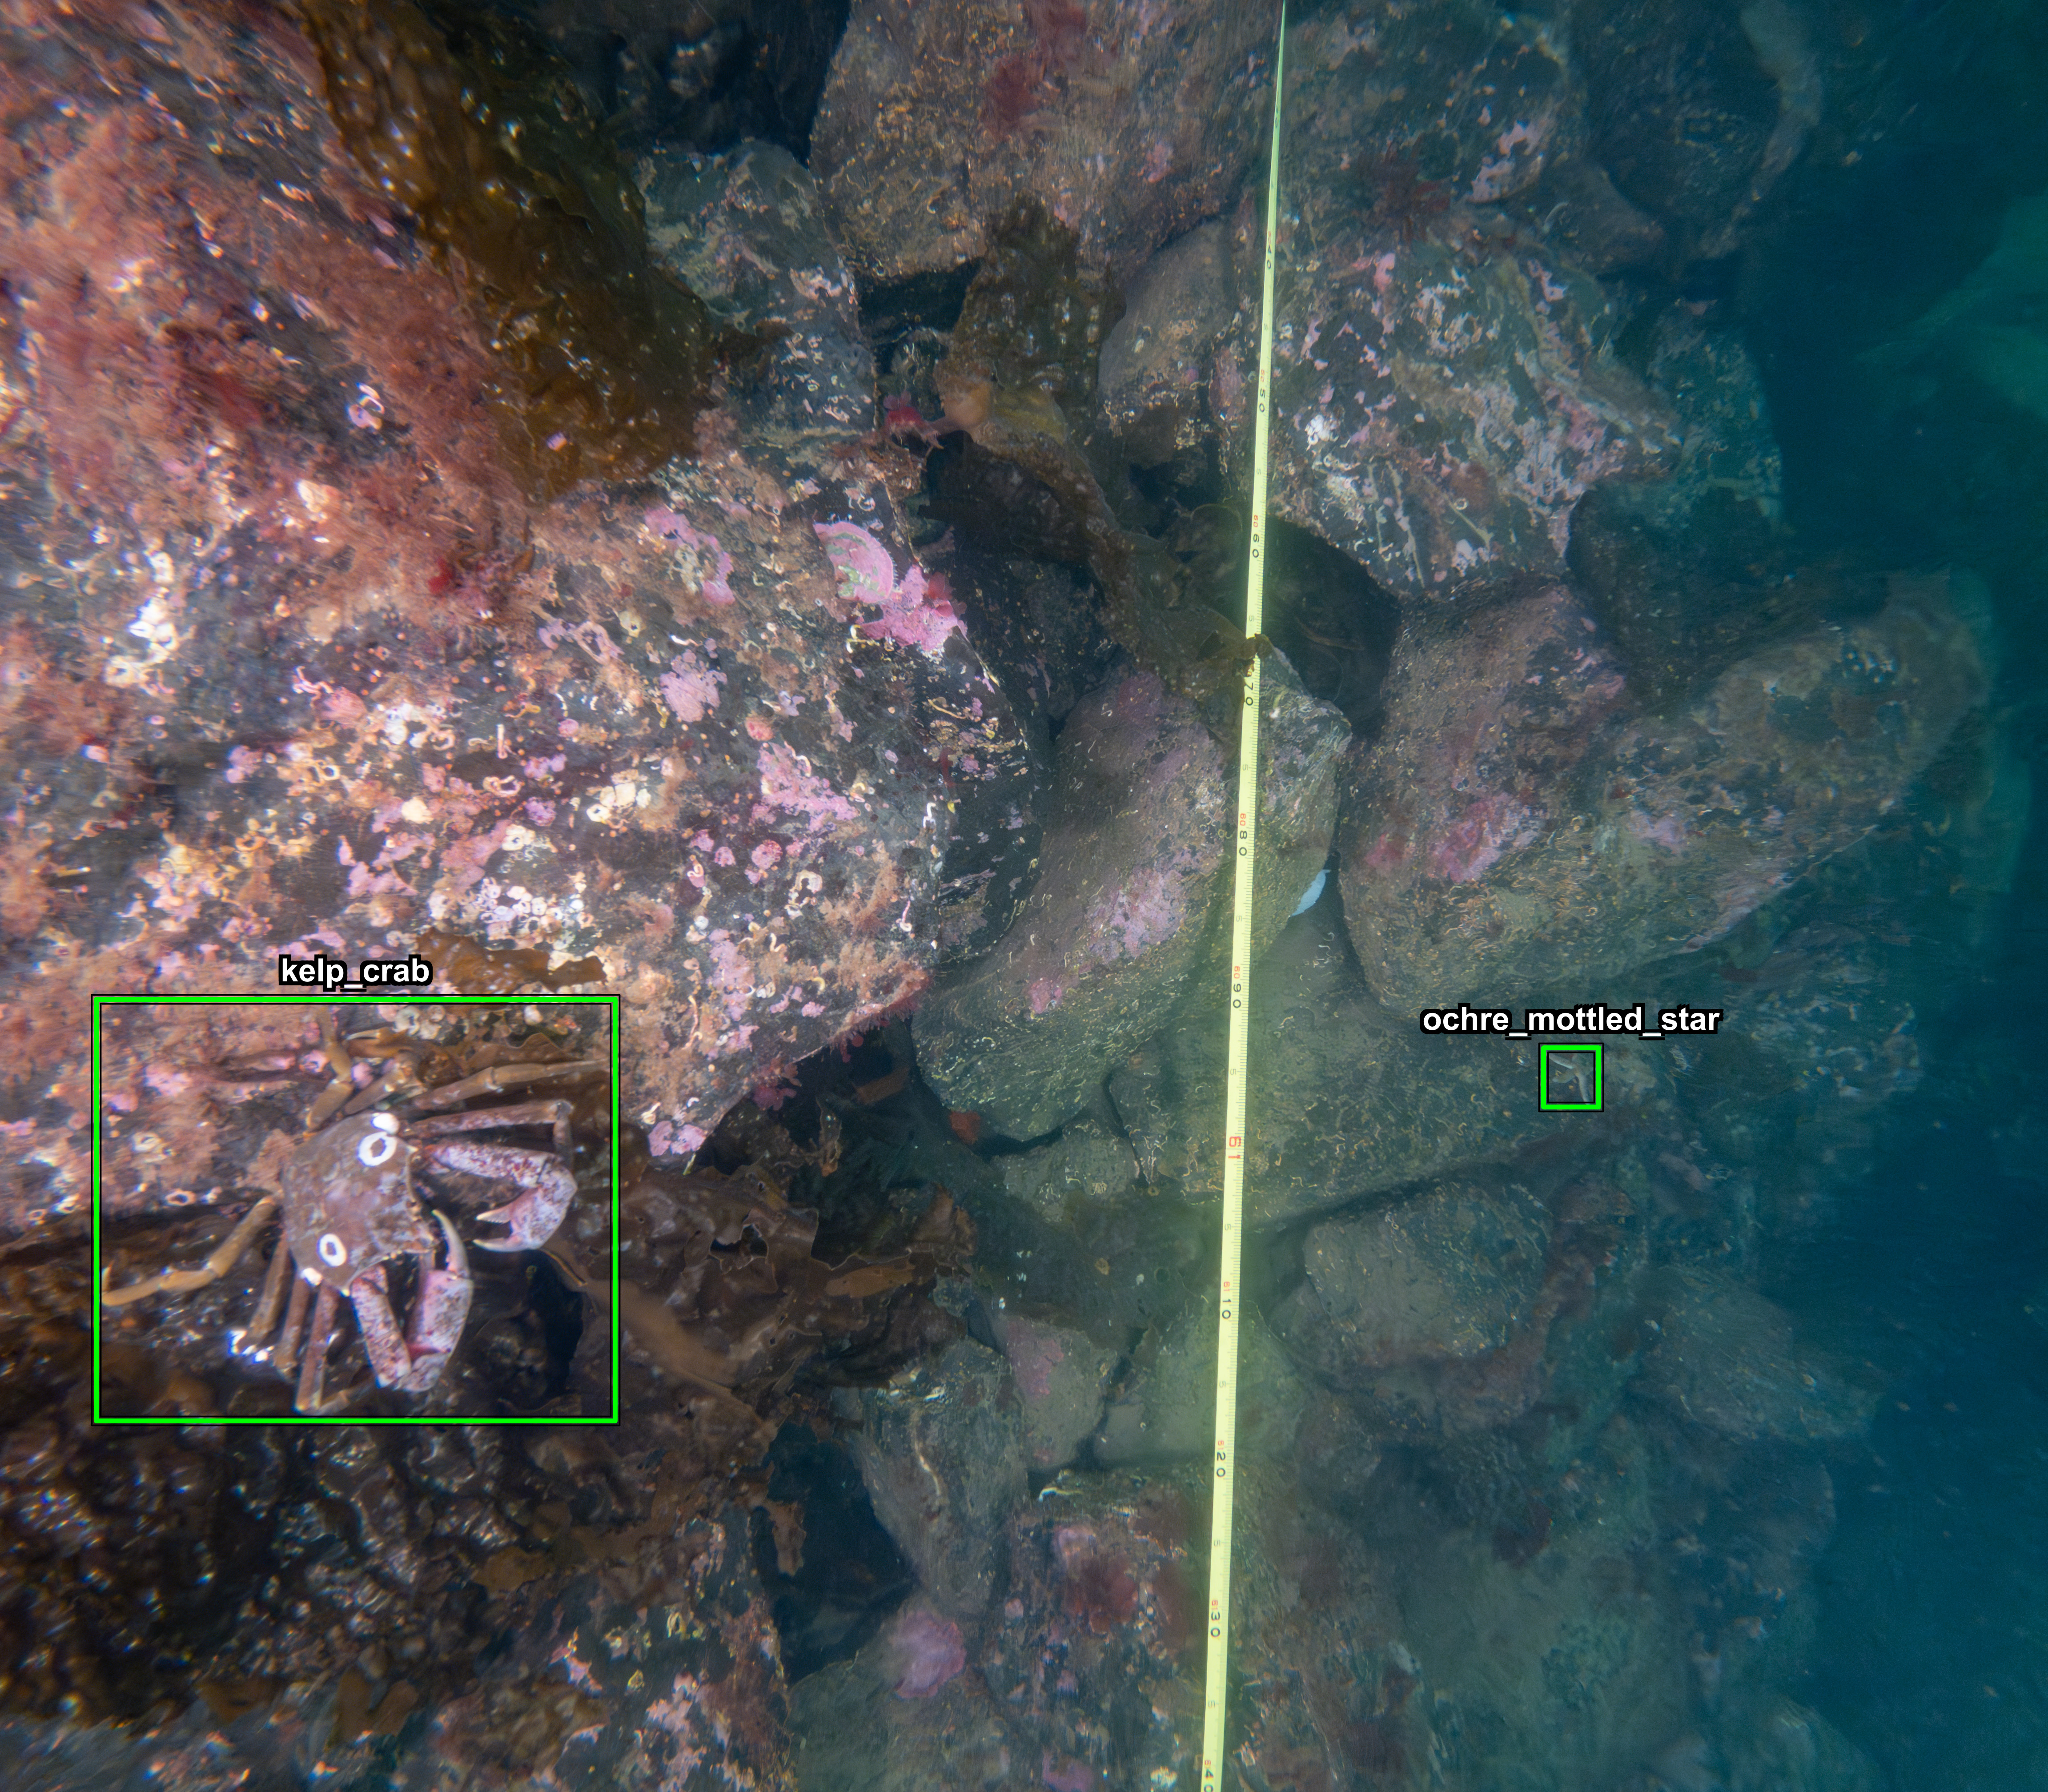
\includegraphics[width=\linewidth]{off_sides_3.jpg}
\end{subfigure}%
\hfill%
\begin{subfigure}[t]{0.495\textwidth}
\centering
\textbf{(d)}\par
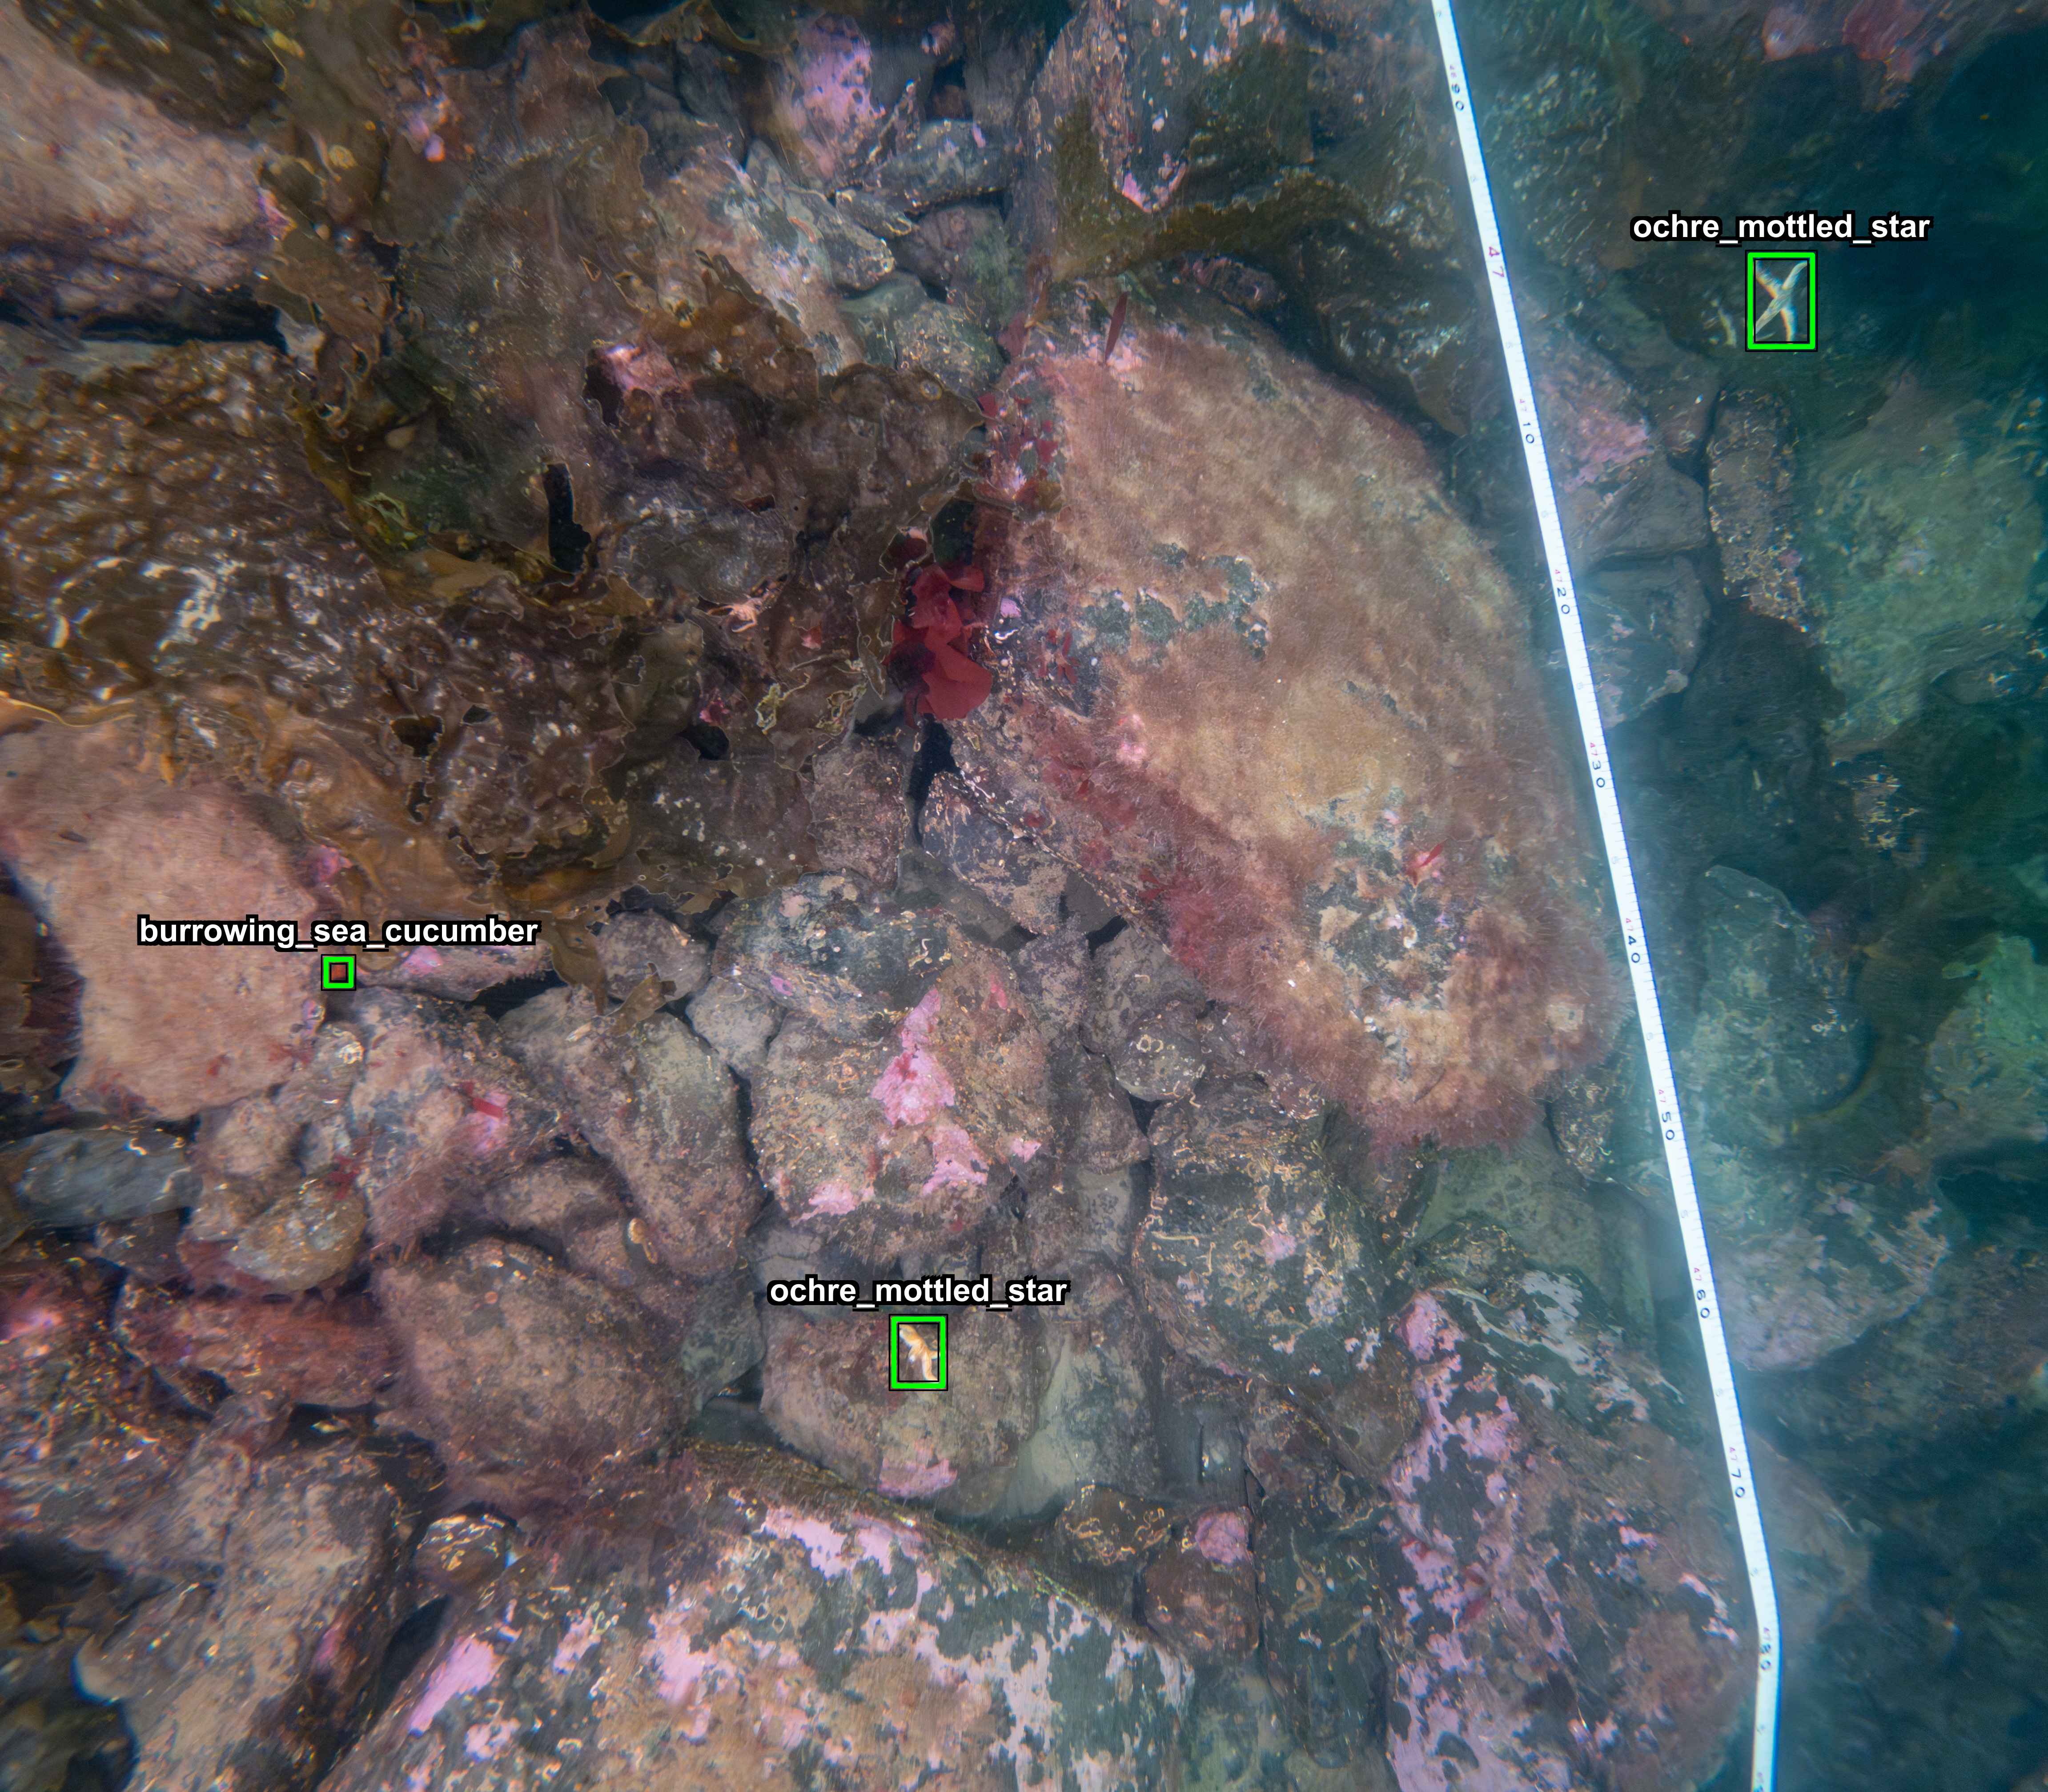
\includegraphics[width=\linewidth]{off_sides_4.jpg}
\end{subfigure}
\caption{
While also relatively rare, there were a few instances where the ROV drifted 
above the transect tape, such that invertebrates were recorded on the ``off
sides'' of the transect;
i.e., invertebrates may have been recorded on the on-shore side of the tape 
when the ROV was surveying the off-shore side of the tape;
as the on-shore side is separately surveyed, this would generate a double-count 
of an invertebrate. 
}
\label{fig:off_sides}
\end{figure}
\vfil
}




%% --------------------------------------------------------------------
%% REFERENCES
%% --------------------------------------------------------------------

\clearpage

% Replace the bibliography style with your preferred style if needed.
\bibliographystyle{../biblio/ecologyLetters}

% Replace this path with the location of your BibTeX database.
\bibliography{../biblio/references}

\end{document}
